% -*- compile-command: "make HOCKING-slides.pdf" -*-
\documentclass{beamer}
\usepackage{tikz}
\usepackage[all]{xy}
\usepackage{amsmath,amssymb}
\usepackage{hyperref}
\usepackage{graphicx}
\usepackage{algorithmic}
\usepackage{multirow}

%\usepackage{appendixnumberbeamer}

\addtobeamertemplate{navigation symbols}{}{%
    \usebeamerfont{footline}%
    \usebeamercolor[fg]{footline}%
    \hspace{1em}%
    \insertframenumber/\inserttotalframenumber
}

\DeclareMathOperator*{\argmin}{arg\,min}
\DeclareMathOperator*{\Lik}{Lik}
\DeclareMathOperator*{\Peaks}{Peaks}
\DeclareMathOperator*{\Segments}{Segments}
\DeclareMathOperator*{\argmax}{arg\,max}
\DeclareMathOperator*{\maximize}{maximize}
\DeclareMathOperator*{\minimize}{minimize}
\newcommand{\sign}{\operatorname{sign}}
\newcommand{\RR}{\mathbb R}
\newcommand{\ZZ}{\mathbb Z}
\newcommand{\NN}{\mathbb N}
\definecolor{pDPA}{HTML}{1B9E77}
\definecolor{PELT}{HTML}{D95F02}
\definecolor{FPOP}{HTML}{7570B3}
\newcommand{\algo}[1]{\textcolor{#1}{#1}}
\definecolor{PDPA}{HTML}{66C2A5}
\definecolor{CDPA}{HTML}{FC8D62}
\definecolor{GPDPA}{HTML}{4D4D4D}




% Set transparency of non-highlighted sections in the table of
% contents slide.
\setbeamertemplate{section in toc shaded}[default][100]
\AtBeginSection[]
{
  \setbeamercolor{section in toc}{fg=red} 
  \setbeamercolor{section in toc shaded}{fg=black} 
  \begin{frame}
    \tableofcontents[currentsection]
  \end{frame}
}

\begin{document}

\title{Statistical machine 
learning algorithms for 
understanding big data in
  genomics and medicine}
\date{10 January 2018}
\author{
  Toby Dylan Hocking\\
  toby.hocking@mail.mcgill.ca
}

\maketitle

\begin{frame}
  \frametitle{Toby Dylan Hocking, brief CV}
  \begin{description}
  \item[2002-2006] UC Berkeley, double major in Molecular Cell Biology
    and Statistics (honors thesis with Terry Speed).
  \item[2006-2008] Biochemistry (DNA-binding specificity of zinc
    finger proteins) and statistics at Sangamo BioSciences.
  \item[2008-2009] Masters in Statistics, Paris 6.
  \item[2009-2012] PhD in Mathematics from Ecole Normale Superieure de
    Cachan, machine learning for cancer genomics with JP Vert (Inst Curie)
    and Francis Bach (INRIA).
  \item[2013] Postdoc in Computer Science (machine learning) with Masashi Sugiyama at Tokyo
    Institute of Technology.
  \item[2014-2017] Postdoc on machine learning for epigenomics
    at McGill with Guillaume Bourque.
  \end{description}
\end{frame}

\section{Introduction to machine learning}

\begin{frame}
  \frametitle{Labeling enables supervised machine learning algorithms}
  \begin{tabular}{ccc}
    Input: Photos & Cell images & Copy number profiles \\
    \includegraphics[width=1.3in]{faces} &
    \includegraphics[width=1.3in]{cellprofiler} &
    \includegraphics[width=1.5in]{regions-axes}\\
    Labels: boxes, names & phenotypes & alterations \\ \\
    %CVPR 2013
%CVPR 2017
Computer vision
 & CellProfiler & SegAnnDB \\
    %246 papers
%783 papers
 & 
%873 citations
%1980 citations
 & H {\it et al.}, 2014. \\
     &
  \end{tabular}
  Sources: \url{http://en.wikipedia.org/wiki/Face_detection}\\
  Jones {\it et al.} PNAS 2009. Scoring diverse cellular morphologies in
  image-based screens with iterative feedback and machine learning.
\end{frame}

\begin{frame}
  \frametitle{Machine learning in computer vision and biology}
  ML is all about learning predictive functions $f(x)\approx y$, where 
  \begin{itemize}
  \item inputs/features $x$ are numerous (e.g. pixels or SNPs).
  \item outputs/labels $y$ are what we want to predict (typically
    phenotypes/classes).
  \item Input $x$ = image of digit,
    output $y\in\{0,1,\dots,9\}$,\\
  $f(\includegraphics[height=1cm]{mnist-0})=0$,
  $f(\includegraphics[height=1cm]{mnist-1})=1$
  % \item Input $x$ = image of article of clothing,\\
  %   output $y\in\{\text{shoe}, \text{pants}, \dots\}$,\\
  % $f(\includegraphics[height=1cm]{fashion-mnist-boot})=\text{shoe}$,
  % $f(\includegraphics[height=1cm]{fashion-mnist-pants})=\text{pants}$
  \item Input $x$ = image of cell, 
    output $y\in\{\text{yes}, \text{no}\}$,\\
  $f(\includegraphics[height=1cm]{cellprofiler-yes})=\text{yes}$,
  $f(\includegraphics[height=1cm]{cellprofiler-no})=\text{no}$
  \item Input $x$ = genomic profile, output $y\in\{\text{breakpoint}, \text{normal}\}$
  $f(\includegraphics[height=1cm]{neuroblastoma-changepoint})=\text{breakpoint}$,
  $f(\includegraphics[height=1cm]{neuroblastoma-nochange})=\text{normal}$
  \end{itemize}
\end{frame}


\begin{frame}
  \frametitle{Supervised machine learning }

  \begin{itemize}
  \item Domain expert labels examples using prior knowledge.
  \item Supervised algorithm learns $f$ based on labeled training data.
  \item State-of-the-art accuracy (if there is enough training data).
  \item Can use same learning algorithm regardless of pattern.
  \end{itemize}

  \begin{center}
      \begin{tabular}{cc}
        \includegraphics[height=1in]{mnist-digits} &
  \includegraphics[height=1in]{fashion-mnist-sprite-some}  
  \end{tabular}
  \end{center}
  
  \vskip -0.2cm
  \scriptsize Sources: github.com/cazala/mnist, github.com/zalandoresearch/fashion-mnist

  \includegraphics[width=\textwidth]{figure-good-bad}
\end{frame}

\begin{frame}
  \frametitle{My main research interests}
  Applications of machine learning in collaboration with domain experts:
  \begin{itemize}
  \item Collaborations: applying machine learning methods to better
    understand/model data from biology and
    medicine.
  \item New labeling methods and benchmark data sets to facilitate
    collaborations between machine learners and domain experts.
  \end{itemize}
  Statistics and machine learning literature (methods development):
  \begin{itemize}
  \item New statistical models for highly accurate pattern
    recognition.
  \item Fast optimization algorithms that scale linearly to huge data
    sets -- important in application domains such as genomics.
  \end{itemize}
\end{frame}

\section{New machine learning algorithms for predicting breakpoint positions in cancer DNA copy number profiles}

\begin{frame}
  \frametitle{Cancer cells show chromosomal copy number alterations}
  Spectral karyotypes show the number of copies of the sex chromosomes
  (X,Y) and autosomes (1-22). 

  Source: Alberts \emph{et al.} 2002.
\vskip 0.1in
  \includegraphics[width=\textwidth]{Karyo-both}
\vskip 0.1in
  \begin{minipage}{0.4\linewidth}
    Normal cell with 2 copies of each autosome.
  \end{minipage}
\hskip 0.1\linewidth
  \begin{minipage}{0.4\linewidth}
Cancer cell with many copy number alterations.
  \end{minipage}
\end{frame}

\begin{frame}
  \frametitle{Breakpoint detection is important in cancers such as
    neuroblastoma } 

  \begin{itemize}
  \item Childhood cancer, most frequently diagnosed at age 1--2.
  \item Top three profiles ``ok'' -- no tumors after initial treatment.
  \item Bottom three ``relapse'' -- aggressive tumor within 5 years.
  \item Previous work: relapse profiles tend to have more breakpoints
     (Schleiermacher {\it et al.}, 2010).
  \end{itemize}

  \includegraphics[width=\textwidth]{neuroblastoma-ok-relapse}
\end{frame}

\begin{frame}
  \frametitle{Breakpoint detection as a machine learning problem}
  
  \begin{itemize}
  \item Input = noisy copy number signal for $p$ probes in one genome
    subset (chromosome).
  \item Output = predict $f(x)\in\{0,1\}^{p-1}$, either a
    \textcolor{green}{breakpoint} (1) or not (0),
    after every data point.
  \item Previous algorithms: unsupervised learning (no labels) --
    collaborators unsatisfied with visually obvious errors.
  \end{itemize}

  \includegraphics[width=\textwidth]{neuroblastoma-ok-relapse-pred}
\end{frame}

\begin{frame}
  \frametitle{New labeling and training methods for breakpoint detection}

  H {\it et al.}, {\it BMC Bioinformatics} 2013.
  \begin{itemize}
  \item Create positive/breakpoint and negative/normal labels.
  \item Quantify/optimize error rate (number of incorrect labels).
  \item Benchmark data set of 3418 chromosomes,
    labeled via visual inspection (R package neuroblastoma).
  \item Results: most accurate model is maximum Gaussian likelihood 
    changepoint detection (cross-validation experiments).
  \end{itemize}

  \includegraphics[width=\textwidth]{neuroblastoma-ok-relapse-supervised}

\end{frame}

\begin{frame}
  \frametitle{Fast FPOP algorithm for computing the maximum likelihood
    changepoint model}

  Maidstone, Hocking, Rigaill, Fearnhead, {\it Stat. and
    Comp.} 2017.

  \begin{itemize}
  \item Naively exponential $O(p^K)$ time to compute best model with
    $K$ segments ($K-1$ changes) for a sequence of $p$ data.
  \item Previous work: other algorithms for computing the model
    (\algo{PELT} and \algo{pDPA}).
  \item Contribution: new log-linear $O(p\log p)$ \algo{FPOP}
    algorithm for computing the same model (R package fpop).
  \end{itemize}
  \begin{center}
    \includegraphics[width=0.5\textwidth]{figure-systemtime-arrays-bins}
  \end{center}
\end{frame}

\begin{frame}
  \frametitle{Supervised interactive DNA copy number analysis}
  H {\it et al.}, {\it Bioinformatics} 2014.

  \begin{itemize}
  \item Previous work: non-interactive command line programs
    -- collaborators can not correct obvious
    errors.
  \item Interactive system: when you edit the labels, the system
    learns and updates the model. (SegAnnDB python module)
  \item Result below: only a few labels required to learn a highly accurate
    breakpoint detection model.
  \end{itemize}
  \begin{minipage}{0.5\linewidth}
    \includegraphics[width=\textwidth]{SegAnnDB-test-error-decreases}
  \end{minipage}
  \begin{minipage}[0.5\linewidth]{0.48\linewidth}
SegAnnDB demo:\\interactively label chr1/chrX
  \url{http://bioviz.rocq.inria.fr/profile/GSM313887/}
  \end{minipage}
\end{frame}

\begin{frame}
  \frametitle{Cancer biology applications}
  Aichi cancer center, Nagoya, Japan.
  \begin{itemize}
  \item Suguro {\it et al.}, {\it Cancer Sci} 2014, Clonal
    heterogeneity of lymphoid malignancies correlates with poor
    prognosis.
  \item Shimada {\it et al.}, {\it Leukemia} 2016, Development and
    analysis of patient-derived xenograft mouse models in
    intravascular large B-cell lymphoma.
  \end{itemize}
  Institut Curie, Paris, France.
  \begin{itemize}
  \item Chicard {\it et al.}, {\it Clinical Cancer Research} 2016,
    Genomic copy number profiling using circulating free tumor DNA
    highlights heterogeneity in neuroblastoma.
  \item Ongoing work, characterizing alterations in neuroblastoma.
  \end{itemize}
\end{frame}

\section{New machine learning algorithms for predicting peaks in ChIP-seq data}

\begin{frame}
  \frametitle{Chromatin immunoprecipitation sequencing (ChIP-seq)}
  Analysis of DNA-protein interactions: which genomic regions have
  bound/modified proteins?

  \includegraphics[width=\textwidth]{Chromatin_immunoprecipitation_sequencing_wide.png}

  Source: ``ChIP-sequencing,'' Wikipedia.
\end{frame}

% \begin{frame}
%   \frametitle{Problem: inaccurate unsupervised peak predictions}
%   \includegraphics[width=\textwidth]{screenshot-ucsc-edited}

%   Grey profiles are normalized aligned read count signals.

%   Black bars are ``peaks'' called by MACS2 (Zhang {\it et al.}, 2008):
%   \begin{itemize}
%   \item many false positives (sometimes false negatives as well).
%   \item overlapping peaks have different start/end positions.
%   \end{itemize}
% \end{frame}

\begin{frame}
  \frametitle{Peak detection as a machine learning problem}

  \includegraphics[width=\textwidth]{screenshot-ucsc-edited}
  
  \begin{itemize}
  \item Input = noisy coverage profile for $n$ bases
    on a chromosome.
  \item Output = predict $f(x)\in\{0,1\}^{n}$ either a peak (1) or not
    (0), for every base.
  \item Previous algorithms: unsupervised learning (no labels) --
    false positives visually obvious.
  \end{itemize}
 
\end{frame} 

% \begin{frame}
%   \frametitle{Previous work in genomic peak detection}
%   \begin{itemize}
%   \item Model-based analysis of ChIP-Seq (MACS), Zhang et al, 2008.
%   \item SICER, Zang et al, 2009.
%   \item HOMER, Heinz et al, 2010.
%   \item CCAT, Xu et al, 2010.
%   \item RSEG, Song et al, 2011.
%   \item Triform, Kornacker et al, 2012.
%   \item Histone modifications in cancer (HMCan), Ashoor et al, 2013.
%   \item PeakSeg, Hocking, Rigaill, Bourque, ICML 2015.
%   \item PeakSegJoint Hocking and Bourque, arXiv:1506.01286.
%   \item ... dozens of others.
%   \end{itemize}
%   Two big questions: how to choose the best...
%   \begin{itemize}
%   \item ...algorithm? (testing)
%   \item ...parameters? (training)
%   \end{itemize}
% \end{frame}

% \begin{frame}[fragile]
%   \frametitle{How to choose parameters of unsupervised peak
%     detectors?}
% \scriptsize
% 19 parameters for Model-based analysis of ChIP-Seq (MACS), Zhang {\it et al.}, 2008.
% \begin{verbatim}
%   [-g GSIZE]
%   [-s TSIZE] [--bw BW] [-m MFOLD MFOLD] [--fix-bimodal]
%   [--nomodel] [--extsize EXTSIZE | --shiftsize SHIFTSIZE]
%   [-q QVALUE | -p PVALUE | -F FOLDENRICHMENT] [--to-large]
%   [--down-sample] [--seed SEED] [--nolambda]
%   [--slocal SMALLLOCAL] [--llocal LARGELOCAL]
%   [--shift-control] [--half-ext] [--broad]
%   [--broad-cutoff BROADCUTOFF] [--call-summits]
% \end{verbatim}
% 10 parameters for Histone modifications in cancer (HMCan),
% Ashoor {\it et al.}, 2013.
% \begin{verbatim}
% minLength 145
% medLength 150
% maxLength 155
% smallBinLength 50
% largeBinLength 100000
% pvalueThreshold 0.01
% mergeDistance 200
% iterationThreshold 5
% finalThreshold 0
% maxIter 20
% \end{verbatim}
% \end{frame}


\begin{frame}
  \frametitle{New labeling method for peak detection in ChIP-seq data}

  H {\it et al.}, {\it Bioinformatics} 2017: choose peak model/parameters
  which minimize the number of incorrectly predicted labels.

  \includegraphics[width=\textwidth]{figure-PeakError.pdf}
  \begin{itemize}
  \item \textbf{peakStart}: exactly one peak start (0=FN, more=FP).
  \item \textbf{peakEnd}: exactly one peak end (0=FN, more=FP).
  \item \textbf{noPeaks}: no overlapping peaks (otherwise FP).
  \item \textbf{peaks}: at least one overlapping peak (otherwise FN).
  \item R package PeakError.
  \end{itemize}
\end{frame}

\begin{frame}
  \frametitle{Only a few labels are required to train highly accurate models to recognize any peak pattern}
  \includegraphics[width=1.1\textwidth]{figure-test-error-decreases-mean.pdf}
 
  \begin{itemize}
  \item Three different ChIP-seq experiments, each with a separate
    labeled pattern (broad/sharp/etc).
  \item Test accuracy quickly increases to max after 2--6
    genomic windows (containing several labeled regions and samples).
  \item PeakSeg highly accurate in all three patterns (H ICML 2015).
  \item Other models only accurate for only one or two patterns.
  \end{itemize}
\end{frame}

\begin{frame}
  \frametitle{PeakSeg is constrained maximum likelihood segmentation}
  H {\it et al.}, {\it ICML} 2015. 

  % Created by tikzDevice version 0.10.1 on 2017-09-15 06:41:33
% !TEX encoding = UTF-8 Unicode
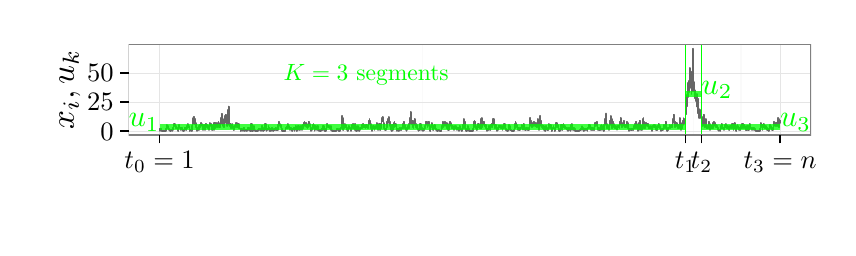
\begin{tikzpicture}[x=1pt,y=1pt]
\definecolor{fillColor}{RGB}{255,255,255}
\path[use as bounding box,fill=fillColor,fill opacity=0.00] (0,0) rectangle (289.08, 72.27);
\begin{scope}
\path[clip] (  0.00,  0.00) rectangle (289.08, 72.27);
\definecolor{drawColor}{RGB}{255,255,255}
\definecolor{fillColor}{RGB}{255,255,255}

\path[draw=drawColor,line width= 0.6pt,line join=round,line cap=round,fill=fillColor] (  0.00, -0.00) rectangle (289.08, 72.27);
\end{scope}
\begin{scope}
\path[clip] ( 36.46, 33.48) rectangle (283.08, 66.27);
\definecolor{fillColor}{RGB}{255,255,255}

\path[fill=fillColor] ( 36.46, 33.48) rectangle (283.08, 66.27);
\definecolor{drawColor}{gray}{0.98}

\path[draw=drawColor,line width= 0.6pt,line join=round] (142.71, 33.48) --
	(142.71, 66.27);

\path[draw=drawColor,line width= 0.6pt,line join=round] (240.61, 33.48) --
	(240.61, 66.27);

\path[draw=drawColor,line width= 0.6pt,line join=round] (257.67, 33.48) --
	(257.67, 66.27);
\definecolor{drawColor}{gray}{0.90}

\path[draw=drawColor,line width= 0.2pt,line join=round] ( 36.46, 34.97) --
	(283.08, 34.97);

\path[draw=drawColor,line width= 0.2pt,line join=round] ( 36.46, 45.46) --
	(283.08, 45.46);

\path[draw=drawColor,line width= 0.2pt,line join=round] ( 36.46, 55.96) --
	(283.08, 55.96);

\path[draw=drawColor,line width= 0.2pt,line join=round] ( 47.67, 33.48) --
	( 47.67, 66.27);

\path[draw=drawColor,line width= 0.2pt,line join=round] (237.74, 33.48) --
	(237.74, 66.27);

\path[draw=drawColor,line width= 0.2pt,line join=round] (243.48, 33.48) --
	(243.48, 66.27);

\path[draw=drawColor,line width= 0.2pt,line join=round] (271.87, 33.48) --
	(271.87, 66.27);
\definecolor{drawColor}{gray}{0.40}

\path[draw=drawColor,line width= 0.6pt,line join=round] ( 47.67, 35.39) --
	( 47.86, 35.39) --
	( 47.86, 34.97) --
	( 47.87, 34.97) --
	( 47.87, 35.39) --
	( 47.88, 35.39) --
	( 47.88, 35.81) --
	( 48.30, 35.81) --
	( 48.30, 35.39) --
	( 48.33, 35.39) --
	( 48.33, 34.97) --
	( 49.90, 34.97) --
	( 49.90, 35.39) --
	( 49.94, 35.39) --
	( 49.94, 35.81) --
	( 50.17, 35.81) --
	( 50.17, 36.23) --
	( 50.24, 36.23) --
	( 50.24, 36.65) --
	( 50.31, 36.65) --
	( 50.31, 37.07) --
	( 50.35, 37.07) --
	( 50.35, 36.65) --
	( 50.39, 36.65) --
	( 50.39, 36.23) --
	( 50.51, 36.23) --
	( 50.51, 36.65) --
	( 50.62, 36.65) --
	( 50.62, 36.23) --
	( 50.68, 36.23) --
	( 50.68, 36.65) --
	( 50.69, 36.65) --
	( 50.69, 36.23) --
	( 50.75, 36.23) --
	( 50.75, 35.81) --
	( 50.96, 35.81) --
	( 50.96, 35.39) --
	( 50.98, 35.39) --
	( 50.98, 35.81) --
	( 51.13, 35.81) --
	( 51.13, 35.39) --
	( 51.43, 35.39) --
	( 51.43, 34.97) --
	( 51.87, 34.97) --
	( 51.87, 35.39) --
	( 52.32, 35.39) --
	( 52.32, 34.97) --
	( 52.35, 34.97) --
	( 52.35, 35.39) --
	( 52.52, 35.39) --
	( 52.52, 35.81) --
	( 52.62, 35.81) --
	( 52.62, 36.23) --
	( 52.70, 36.23) --
	( 52.70, 36.65) --
	( 52.72, 36.65) --
	( 52.72, 37.07) --
	( 52.80, 37.07) --
	( 52.80, 36.65) --
	( 52.85, 36.65) --
	( 52.85, 37.07) --
	( 52.95, 37.07) --
	( 52.95, 37.49) --
	( 52.97, 37.49) --
	( 52.97, 37.07) --
	( 52.97, 37.07) --
	( 52.97, 37.49) --
	( 53.06, 37.49) --
	( 53.06, 37.07) --
	( 53.13, 37.07) --
	( 53.13, 37.49) --
	( 53.15, 37.49) --
	( 53.15, 37.07) --
	( 53.16, 37.07) --
	( 53.16, 36.65) --
	( 53.18, 36.65) --
	( 53.18, 37.07) --
	( 53.30, 37.07) --
	( 53.30, 36.65) --
	( 53.40, 36.65) --
	( 53.40, 36.23) --
	( 53.42, 36.23) --
	( 53.42, 35.81) --
	( 53.45, 35.81) --
	( 53.45, 36.23) --
	( 53.47, 36.23) --
	( 53.47, 36.65) --
	( 53.58, 36.65) --
	( 53.58, 36.23) --
	( 53.62, 36.23) --
	( 53.62, 35.81) --
	( 53.90, 35.81) --
	( 53.90, 36.23) --
	( 53.92, 36.23) --
	( 53.92, 35.81) --
	( 54.35, 35.81) --
	( 54.35, 34.97) --
	( 54.45, 34.97) --
	( 54.45, 35.39) --
	( 54.48, 35.39) --
	( 54.48, 35.81) --
	( 54.53, 35.81) --
	( 54.53, 36.23) --
	( 54.66, 36.23) --
	( 54.66, 36.65) --
	( 54.74, 36.65) --
	( 54.74, 37.07) --
	( 54.90, 37.07) --
	( 54.90, 36.65) --
	( 54.92, 36.65) --
	( 54.92, 36.23) --
	( 54.97, 36.23) --
	( 54.97, 35.81) --
	( 54.98, 35.81) --
	( 54.98, 36.23) --
	( 55.11, 36.23) --
	( 55.11, 35.81) --
	( 55.18, 35.81) --
	( 55.18, 35.39) --
	( 55.23, 35.39) --
	( 55.23, 35.81) --
	( 55.32, 35.81) --
	( 55.32, 36.23) --
	( 55.42, 36.23) --
	( 55.42, 35.81) --
	( 55.61, 35.81) --
	( 55.61, 36.23) --
	( 55.68, 36.23) --
	( 55.68, 35.81) --
	( 55.77, 35.81) --
	( 55.77, 35.39) --
	( 56.06, 35.39) --
	( 56.06, 34.97) --
	( 56.42, 34.97) --
	( 56.42, 35.39) --
	( 56.65, 35.39) --
	( 56.65, 35.81) --
	( 56.71, 35.81) --
	( 56.71, 36.23) --
	( 56.87, 36.23) --
	( 56.87, 35.81) --
	( 56.97, 35.81) --
	( 56.97, 36.23) --
	( 57.10, 36.23) --
	( 57.10, 35.81) --
	( 57.16, 35.81) --
	( 57.16, 35.39) --
	( 57.40, 35.39) --
	( 57.40, 35.81) --
	( 57.42, 35.81) --
	( 57.42, 35.39) --
	( 57.43, 35.39) --
	( 57.43, 35.81) --
	( 57.60, 35.81) --
	( 57.60, 36.65) --
	( 57.78, 36.65) --
	( 57.78, 37.07) --
	( 57.84, 37.07) --
	( 57.84, 36.65) --
	( 57.88, 36.65) --
	( 57.88, 36.23) --
	( 58.02, 36.23) --
	( 58.02, 37.07) --
	( 58.04, 37.07) --
	( 58.04, 37.49) --
	( 58.05, 37.49) --
	( 58.05, 36.65) --
	( 58.23, 36.65) --
	( 58.23, 36.23) --
	( 58.47, 36.23) --
	( 58.47, 35.39) --
	( 58.48, 35.39) --
	( 58.48, 34.97) --
	( 58.74, 34.97) --
	( 58.74, 35.39) --
	( 59.18, 35.39) --
	( 59.18, 34.97) --
	( 59.31, 34.97) --
	( 59.31, 35.39) --
	( 59.37, 35.39) --
	( 59.37, 35.81) --
	( 59.42, 35.81) --
	( 59.42, 36.65) --
	( 59.51, 36.65) --
	( 59.51, 37.49) --
	( 59.65, 37.49) --
	( 59.65, 37.91) --
	( 59.69, 37.91) --
	( 59.69, 38.33) --
	( 59.76, 38.33) --
	( 59.76, 37.91) --
	( 59.79, 37.91) --
	( 59.79, 39.17) --
	( 59.81, 39.17) --
	( 59.81, 39.59) --
	( 59.81, 39.59) --
	( 59.81, 39.17) --
	( 59.86, 39.17) --
	( 59.86, 40.01) --
	( 59.87, 40.01) --
	( 59.87, 39.17) --
	( 59.93, 39.17) --
	( 59.93, 39.59) --
	( 59.96, 39.59) --
	( 59.96, 38.75) --
	( 60.02, 38.75) --
	( 60.02, 39.17) --
	( 60.10, 39.17) --
	( 60.10, 38.75) --
	( 60.14, 38.75) --
	( 60.14, 38.33) --
	( 60.18, 38.33) --
	( 60.18, 39.59) --
	( 60.22, 39.59) --
	( 60.22, 40.01) --
	( 60.24, 40.01) --
	( 60.24, 39.59) --
	( 60.24, 39.59) --
	( 60.24, 38.75) --
	( 60.26, 38.75) --
	( 60.26, 38.33) --
	( 60.31, 38.33) --
	( 60.31, 37.49) --
	( 60.40, 37.49) --
	( 60.40, 37.91) --
	( 60.42, 37.91) --
	( 60.42, 38.33) --
	( 60.43, 38.33) --
	( 60.43, 38.75) --
	( 60.47, 38.75) --
	( 60.47, 38.33) --
	( 60.58, 38.33) --
	( 60.58, 38.75) --
	( 60.60, 38.75) --
	( 60.60, 39.17) --
	( 60.63, 39.17) --
	( 60.63, 37.91) --
	( 60.64, 37.91) --
	( 60.64, 38.33) --
	( 60.67, 38.33) --
	( 60.67, 37.91) --
	( 60.83, 37.91) --
	( 60.83, 37.49) --
	( 60.85, 37.49) --
	( 60.85, 37.07) --
	( 60.87, 37.07) --
	( 60.87, 36.23) --
	( 61.03, 36.23) --
	( 61.03, 35.39) --
	( 61.09, 35.39) --
	( 61.09, 34.97) --
	( 61.14, 34.97) --
	( 61.14, 35.39) --
	( 61.22, 35.39) --
	( 61.22, 35.81) --
	( 61.44, 35.81) --
	( 61.44, 36.23) --
	( 61.58, 36.23) --
	( 61.58, 35.81) --
	( 61.67, 35.81) --
	( 61.67, 35.39) --
	( 61.79, 35.39) --
	( 61.79, 35.81) --
	( 61.89, 35.81) --
	( 61.89, 35.39) --
	( 61.90, 35.39) --
	( 61.90, 35.81) --
	( 61.94, 35.81) --
	( 61.94, 36.23) --
	( 61.96, 36.23) --
	( 61.96, 36.65) --
	( 62.13, 36.65) --
	( 62.13, 37.07) --
	( 62.24, 37.07) --
	( 62.24, 36.65) --
	( 62.26, 36.65) --
	( 62.26, 37.07) --
	( 62.35, 37.07) --
	( 62.35, 36.65) --
	( 62.39, 36.65) --
	( 62.39, 36.23) --
	( 62.40, 36.23) --
	( 62.40, 37.07) --
	( 62.41, 37.07) --
	( 62.41, 36.65) --
	( 62.49, 36.65) --
	( 62.49, 37.07) --
	( 62.50, 37.07) --
	( 62.50, 37.49) --
	( 62.65, 37.49) --
	( 62.65, 37.91) --
	( 62.70, 37.91) --
	( 62.70, 37.49) --
	( 62.79, 37.49) --
	( 62.79, 37.91) --
	( 62.84, 37.91) --
	( 62.84, 37.07) --
	( 62.93, 37.07) --
	( 62.93, 37.49) --
	( 62.94, 37.49) --
	( 62.94, 37.07) --
	( 62.95, 37.07) --
	( 62.95, 36.65) --
	( 62.99, 36.65) --
	( 62.99, 37.49) --
	( 63.02, 37.49) --
	( 63.02, 37.07) --
	( 63.10, 37.07) --
	( 63.10, 36.65) --
	( 63.24, 36.65) --
	( 63.24, 36.23) --
	( 63.35, 36.23) --
	( 63.35, 36.65) --
	( 63.38, 36.65) --
	( 63.38, 36.23) --
	( 63.44, 36.23) --
	( 63.44, 35.39) --
	( 63.45, 35.39) --
	( 63.45, 35.81) --
	( 63.47, 35.81) --
	( 63.47, 36.23) --
	( 63.52, 36.23) --
	( 63.52, 36.65) --
	( 63.77, 36.65) --
	( 63.77, 37.07) --
	( 63.79, 37.07) --
	( 63.79, 36.65) --
	( 63.90, 36.65) --
	( 63.90, 36.23) --
	( 63.92, 36.23) --
	( 63.92, 35.81) --
	( 63.97, 35.81) --
	( 63.97, 35.39) --
	( 64.05, 35.39) --
	( 64.05, 35.81) --
	( 64.16, 35.81) --
	( 64.16, 36.23) --
	( 64.18, 36.23) --
	( 64.18, 36.65) --
	( 64.19, 36.65) --
	( 64.19, 37.07) --
	( 64.22, 37.07) --
	( 64.22, 36.65) --
	( 64.23, 36.65) --
	( 64.23, 37.07) --
	( 64.30, 37.07) --
	( 64.30, 37.49) --
	( 64.50, 37.49) --
	( 64.50, 37.07) --
	( 64.58, 37.07) --
	( 64.58, 37.49) --
	( 64.63, 37.49) --
	( 64.63, 37.07) --
	( 64.64, 37.07) --
	( 64.64, 36.65) --
	( 64.65, 36.65) --
	( 64.65, 37.07) --
	( 64.68, 37.07) --
	( 64.68, 36.65) --
	( 64.74, 36.65) --
	( 64.74, 36.23) --
	( 64.96, 36.23) --
	( 64.96, 36.65) --
	( 65.00, 36.65) --
	( 65.00, 37.07) --
	( 65.03, 37.07) --
	( 65.03, 36.65) --
	( 65.05, 36.65) --
	( 65.05, 36.23) --
	( 65.09, 36.23) --
	( 65.09, 35.81) --
	( 65.39, 35.81) --
	( 65.39, 36.23) --
	( 65.41, 36.23) --
	( 65.41, 35.81) --
	( 65.44, 35.81) --
	( 65.44, 35.39) --
	( 65.50, 35.39) --
	( 65.50, 35.81) --
	( 65.51, 35.81) --
	( 65.51, 36.23) --
	( 65.60, 36.23) --
	( 65.60, 36.65) --
	( 65.68, 36.65) --
	( 65.68, 37.07) --
	( 65.70, 37.07) --
	( 65.70, 37.49) --
	( 65.79, 37.49) --
	( 65.79, 37.91) --
	( 65.84, 37.91) --
	( 65.84, 37.49) --
	( 65.93, 37.49) --
	( 65.93, 37.91) --
	( 65.94, 37.91) --
	( 65.94, 37.49) --
	( 65.95, 37.49) --
	( 65.95, 37.07) --
	( 66.01, 37.07) --
	( 66.01, 36.65) --
	( 66.05, 36.65) --
	( 66.05, 37.07) --
	( 66.12, 37.07) --
	( 66.12, 37.49) --
	( 66.13, 37.49) --
	( 66.13, 37.07) --
	( 66.13, 37.07) --
	( 66.13, 37.49) --
	( 66.15, 37.49) --
	( 66.15, 37.07) --
	( 66.18, 37.07) --
	( 66.18, 37.49) --
	( 66.24, 37.49) --
	( 66.24, 37.07) --
	( 66.30, 37.07) --
	( 66.30, 37.49) --
	( 66.38, 37.49) --
	( 66.38, 37.07) --
	( 66.50, 37.07) --
	( 66.50, 36.65) --
	( 66.57, 36.65) --
	( 66.57, 36.23) --
	( 66.58, 36.23) --
	( 66.58, 35.81) --
	( 66.63, 35.81) --
	( 66.63, 35.39) --
	( 66.65, 35.39) --
	( 66.65, 35.81) --
	( 66.67, 35.81) --
	( 66.67, 35.39) --
	( 66.81, 35.39) --
	( 66.81, 35.81) --
	( 67.05, 35.81) --
	( 67.05, 36.23) --
	( 67.10, 36.23) --
	( 67.10, 35.81) --
	( 67.26, 35.81) --
	( 67.26, 35.39) --
	( 67.28, 35.39) --
	( 67.28, 36.23) --
	( 67.30, 36.23) --
	( 67.30, 36.65) --
	( 67.32, 36.65) --
	( 67.32, 37.07) --
	( 67.34, 37.07) --
	( 67.34, 37.49) --
	( 67.38, 37.49) --
	( 67.38, 37.91) --
	( 67.50, 37.91) --
	( 67.50, 37.49) --
	( 67.57, 37.49) --
	( 67.57, 37.91) --
	( 67.73, 37.91) --
	( 67.73, 37.07) --
	( 67.75, 37.07) --
	( 67.75, 36.65) --
	( 67.76, 36.65) --
	( 67.76, 36.23) --
	( 67.82, 36.23) --
	( 67.82, 35.81) --
	( 67.91, 35.81) --
	( 67.91, 36.23) --
	( 67.93, 36.23) --
	( 67.93, 37.07) --
	( 68.05, 37.07) --
	( 68.05, 37.49) --
	( 68.09, 37.49) --
	( 68.09, 37.91) --
	( 68.24, 37.91) --
	( 68.24, 37.49) --
	( 68.35, 37.49) --
	( 68.35, 37.07) --
	( 68.38, 37.07) --
	( 68.38, 36.23) --
	( 68.40, 36.23) --
	( 68.40, 36.65) --
	( 68.47, 36.65) --
	( 68.47, 36.23) --
	( 68.49, 36.23) --
	( 68.49, 36.65) --
	( 68.50, 36.65) --
	( 68.50, 36.23) --
	( 68.53, 36.23) --
	( 68.53, 36.65) --
	( 68.54, 36.65) --
	( 68.54, 36.23) --
	( 68.60, 36.23) --
	( 68.60, 36.65) --
	( 68.67, 36.65) --
	( 68.67, 37.07) --
	( 68.70, 37.07) --
	( 68.70, 37.49) --
	( 68.78, 37.49) --
	( 68.78, 37.91) --
	( 68.85, 37.91) --
	( 68.85, 37.49) --
	( 68.85, 37.49) --
	( 68.85, 37.91) --
	( 68.94, 37.91) --
	( 68.94, 37.49) --
	( 68.97, 37.49) --
	( 68.97, 37.91) --
	( 68.97, 37.91) --
	( 68.97, 38.33) --
	( 68.98, 38.33) --
	( 68.98, 37.91) --
	( 69.04, 37.91) --
	( 69.04, 37.49) --
	( 69.12, 37.49) --
	( 69.12, 37.07) --
	( 69.15, 37.07) --
	( 69.15, 36.65) --
	( 69.22, 36.65) --
	( 69.22, 36.23) --
	( 69.23, 36.23) --
	( 69.23, 36.65) --
	( 69.26, 36.65) --
	( 69.26, 37.49) --
	( 69.30, 37.49) --
	( 69.30, 37.07) --
	( 69.42, 37.07) --
	( 69.42, 36.65) --
	( 69.42, 36.65) --
	( 69.42, 36.23) --
	( 69.44, 36.23) --
	( 69.44, 36.65) --
	( 69.49, 36.65) --
	( 69.49, 37.07) --
	( 69.56, 37.07) --
	( 69.56, 37.49) --
	( 69.66, 37.49) --
	( 69.66, 37.91) --
	( 69.68, 37.91) --
	( 69.68, 37.49) --
	( 69.69, 37.49) --
	( 69.69, 37.91) --
	( 69.70, 37.91) --
	( 69.70, 38.33) --
	( 69.71, 38.33) --
	( 69.71, 37.91) --
	( 69.71, 37.91) --
	( 69.71, 37.49) --
	( 69.74, 37.49) --
	( 69.74, 37.91) --
	( 69.88, 37.91) --
	( 69.88, 38.33) --
	( 69.89, 38.33) --
	( 69.89, 37.91) --
	( 69.93, 37.91) --
	( 69.93, 38.33) --
	( 69.94, 38.33) --
	( 69.94, 37.91) --
	( 69.96, 37.91) --
	( 69.96, 39.17) --
	( 69.96, 39.17) --
	( 69.96, 39.59) --
	( 69.99, 39.59) --
	( 69.99, 39.17) --
	( 70.01, 39.17) --
	( 70.01, 39.59) --
	( 70.05, 39.59) --
	( 70.05, 40.01) --
	( 70.09, 40.01) --
	( 70.09, 40.43) --
	( 70.11, 40.43) --
	( 70.11, 40.01) --
	( 70.14, 40.01) --
	( 70.14, 39.59) --
	( 70.15, 39.59) --
	( 70.15, 39.17) --
	( 70.16, 39.17) --
	( 70.16, 39.59) --
	( 70.18, 39.59) --
	( 70.18, 40.01) --
	( 70.19, 40.01) --
	( 70.19, 39.59) --
	( 70.20, 39.59) --
	( 70.20, 40.43) --
	( 70.26, 40.43) --
	( 70.26, 40.85) --
	( 70.32, 40.85) --
	( 70.32, 41.27) --
	( 70.33, 41.27) --
	( 70.33, 40.85) --
	( 70.38, 40.85) --
	( 70.38, 40.43) --
	( 70.41, 40.43) --
	( 70.41, 39.17) --
	( 70.41, 39.17) --
	( 70.41, 38.33) --
	( 70.43, 38.33) --
	( 70.43, 38.75) --
	( 70.48, 38.75) --
	( 70.48, 39.17) --
	( 70.50, 39.17) --
	( 70.50, 38.75) --
	( 70.54, 38.75) --
	( 70.54, 38.33) --
	( 70.56, 38.33) --
	( 70.56, 37.91) --
	( 70.63, 37.91) --
	( 70.63, 37.49) --
	( 70.65, 37.49) --
	( 70.65, 36.65) --
	( 70.69, 36.65) --
	( 70.69, 37.07) --
	( 70.70, 37.07) --
	( 70.70, 36.23) --
	( 70.79, 36.23) --
	( 70.79, 36.65) --
	( 70.87, 36.65) --
	( 70.87, 37.07) --
	( 70.87, 37.07) --
	( 70.87, 36.65) --
	( 70.93, 36.65) --
	( 70.93, 36.23) --
	( 71.00, 36.23) --
	( 71.00, 37.07) --
	( 71.04, 37.07) --
	( 71.04, 37.49) --
	( 71.08, 37.49) --
	( 71.08, 37.91) --
	( 71.08, 37.91) --
	( 71.08, 37.49) --
	( 71.15, 37.49) --
	( 71.15, 37.91) --
	( 71.17, 37.91) --
	( 71.17, 38.33) --
	( 71.24, 38.33) --
	( 71.24, 37.91) --
	( 71.27, 37.91) --
	( 71.27, 38.33) --
	( 71.27, 38.33) --
	( 71.27, 38.75) --
	( 71.31, 38.75) --
	( 71.31, 39.17) --
	( 71.33, 39.17) --
	( 71.33, 38.75) --
	( 71.35, 38.75) --
	( 71.35, 39.17) --
	( 71.39, 39.17) --
	( 71.39, 39.59) --
	( 71.40, 39.59) --
	( 71.40, 40.01) --
	( 71.41, 40.01) --
	( 71.41, 40.43) --
	( 71.46, 40.43) --
	( 71.46, 40.85) --
	( 71.48, 40.85) --
	( 71.48, 40.43) --
	( 71.51, 40.43) --
	( 71.51, 40.85) --
	( 71.52, 40.85) --
	( 71.52, 40.43) --
	( 71.53, 40.43) --
	( 71.53, 40.01) --
	( 71.56, 40.01) --
	( 71.56, 40.43) --
	( 71.57, 40.43) --
	( 71.57, 40.85) --
	( 71.60, 40.85) --
	( 71.60, 40.43) --
	( 71.67, 40.43) --
	( 71.67, 40.85) --
	( 71.72, 40.85) --
	( 71.72, 40.43) --
	( 71.75, 40.43) --
	( 71.75, 40.01) --
	( 71.76, 40.01) --
	( 71.76, 40.43) --
	( 71.77, 40.43) --
	( 71.77, 40.01) --
	( 71.80, 40.01) --
	( 71.80, 40.43) --
	( 71.83, 40.43) --
	( 71.83, 40.01) --
	( 71.85, 40.01) --
	( 71.85, 39.59) --
	( 71.86, 39.59) --
	( 71.86, 39.17) --
	( 71.89, 39.17) --
	( 71.89, 38.75) --
	( 71.91, 38.75) --
	( 71.91, 38.33) --
	( 71.95, 38.33) --
	( 71.95, 37.91) --
	( 72.00, 37.91) --
	( 72.00, 37.49) --
	( 72.00, 37.49) --
	( 72.00, 37.91) --
	( 72.01, 37.91) --
	( 72.01, 37.49) --
	( 72.02, 37.49) --
	( 72.02, 37.07) --
	( 72.07, 37.07) --
	( 72.07, 36.65) --
	( 72.08, 36.65) --
	( 72.08, 37.07) --
	( 72.11, 37.07) --
	( 72.11, 37.49) --
	( 72.12, 37.49) --
	( 72.12, 37.07) --
	( 72.19, 37.07) --
	( 72.19, 37.49) --
	( 72.21, 37.49) --
	( 72.21, 37.07) --
	( 72.25, 37.07) --
	( 72.25, 36.65) --
	( 72.26, 36.65) --
	( 72.26, 37.07) --
	( 72.27, 37.07) --
	( 72.27, 37.91) --
	( 72.28, 37.91) --
	( 72.28, 38.33) --
	( 72.34, 38.33) --
	( 72.34, 38.75) --
	( 72.37, 38.75) --
	( 72.37, 39.17) --
	( 72.38, 39.17) --
	( 72.38, 39.59) --
	( 72.39, 39.59) --
	( 72.39, 40.01) --
	( 72.43, 40.01) --
	( 72.43, 40.43) --
	( 72.44, 40.43) --
	( 72.44, 40.85) --
	( 72.45, 40.85) --
	( 72.45, 40.43) --
	( 72.46, 40.43) --
	( 72.46, 40.85) --
	( 72.47, 40.85) --
	( 72.47, 42.11) --
	( 72.49, 42.11) --
	( 72.49, 42.53) --
	( 72.51, 42.53) --
	( 72.51, 42.11) --
	( 72.52, 42.11) --
	( 72.52, 42.53) --
	( 72.53, 42.53) --
	( 72.53, 42.94) --
	( 72.55, 42.94) --
	( 72.55, 43.36) --
	( 72.56, 43.36) --
	( 72.56, 43.78) --
	( 72.56, 43.78) --
	( 72.56, 43.36) --
	( 72.61, 43.36) --
	( 72.61, 43.78) --
	( 72.64, 43.78) --
	( 72.64, 43.36) --
	( 72.71, 43.36) --
	( 72.71, 42.94) --
	( 72.72, 42.94) --
	( 72.72, 42.53) --
	( 72.73, 42.53) --
	( 72.73, 42.11) --
	( 72.78, 42.11) --
	( 72.78, 41.69) --
	( 72.82, 41.69) --
	( 72.82, 41.27) --
	( 72.83, 41.27) --
	( 72.83, 40.85) --
	( 72.83, 40.85) --
	( 72.83, 40.43) --
	( 72.87, 40.43) --
	( 72.87, 40.01) --
	( 72.89, 40.01) --
	( 72.89, 39.59) --
	( 72.91, 39.59) --
	( 72.91, 39.17) --
	( 72.92, 39.17) --
	( 72.92, 37.91) --
	( 72.93, 37.91) --
	( 72.93, 38.33) --
	( 72.94, 38.33) --
	( 72.94, 37.49) --
	( 72.97, 37.49) --
	( 72.97, 37.07) --
	( 72.98, 37.07) --
	( 72.98, 36.65) --
	( 72.99, 36.65) --
	( 72.99, 37.07) --
	( 72.99, 37.07) --
	( 72.99, 37.49) --
	( 73.01, 37.49) --
	( 73.01, 37.07) --
	( 73.06, 37.07) --
	( 73.06, 36.65) --
	( 73.18, 36.65) --
	( 73.18, 37.49) --
	( 73.38, 37.49) --
	( 73.38, 37.07) --
	( 73.44, 37.07) --
	( 73.44, 35.81) --
	( 73.60, 35.81) --
	( 73.60, 36.65) --
	( 73.63, 36.65) --
	( 73.63, 35.81) --
	( 73.71, 35.81) --
	( 73.71, 36.23) --
	( 73.84, 36.23) --
	( 73.84, 36.65) --
	( 73.98, 36.65) --
	( 73.98, 37.07) --
	( 73.99, 37.07) --
	( 73.99, 37.49) --
	( 74.05, 37.49) --
	( 74.05, 36.65) --
	( 74.15, 36.65) --
	( 74.15, 36.23) --
	( 74.29, 36.23) --
	( 74.29, 35.81) --
	( 74.30, 35.81) --
	( 74.30, 36.23) --
	( 74.43, 36.23) --
	( 74.43, 35.81) --
	( 74.43, 35.81) --
	( 74.43, 35.39) --
	( 74.46, 35.39) --
	( 74.46, 35.81) --
	( 74.46, 35.81) --
	( 74.46, 36.23) --
	( 74.73, 36.23) --
	( 74.73, 36.65) --
	( 74.74, 36.65) --
	( 74.74, 36.23) --
	( 74.88, 36.23) --
	( 74.88, 36.65) --
	( 74.91, 36.65) --
	( 74.91, 36.23) --
	( 74.98, 36.23) --
	( 74.98, 36.65) --
	( 75.11, 36.65) --
	( 75.11, 37.07) --
	( 75.18, 37.07) --
	( 75.18, 36.65) --
	( 75.22, 36.65) --
	( 75.22, 37.07) --
	( 75.28, 37.07) --
	( 75.28, 37.91) --
	( 75.33, 37.91) --
	( 75.33, 37.49) --
	( 75.35, 37.49) --
	( 75.35, 37.07) --
	( 75.43, 37.07) --
	( 75.43, 36.65) --
	( 75.48, 36.65) --
	( 75.48, 37.07) --
	( 75.49, 37.07) --
	( 75.49, 37.49) --
	( 75.56, 37.49) --
	( 75.56, 37.07) --
	( 75.60, 37.07) --
	( 75.60, 37.49) --
	( 75.64, 37.49) --
	( 75.64, 37.91) --
	( 75.65, 37.91) --
	( 75.65, 37.49) --
	( 75.66, 37.49) --
	( 75.66, 37.07) --
	( 75.69, 37.07) --
	( 75.69, 36.65) --
	( 75.72, 36.65) --
	( 75.72, 36.23) --
	( 75.80, 36.23) --
	( 75.80, 36.65) --
	( 75.82, 36.65) --
	( 75.82, 37.07) --
	( 75.86, 37.07) --
	( 75.86, 36.65) --
	( 75.94, 36.65) --
	( 75.94, 36.23) --
	( 75.96, 36.23) --
	( 75.96, 36.65) --
	( 75.96, 36.65) --
	( 75.96, 37.07) --
	( 76.06, 37.07) --
	( 76.06, 37.49) --
	( 76.09, 37.49) --
	( 76.09, 37.07) --
	( 76.09, 37.07) --
	( 76.09, 37.49) --
	( 76.25, 37.49) --
	( 76.25, 37.07) --
	( 76.27, 37.07) --
	( 76.27, 36.65) --
	( 76.40, 36.65) --
	( 76.40, 35.81) --
	( 76.48, 35.81) --
	( 76.48, 36.23) --
	( 76.51, 36.23) --
	( 76.51, 35.81) --
	( 76.51, 35.81) --
	( 76.51, 36.23) --
	( 76.54, 36.23) --
	( 76.54, 35.81) --
	( 76.93, 35.81) --
	( 76.93, 35.39) --
	( 76.96, 35.39) --
	( 76.96, 34.97) --
	( 77.15, 34.97) --
	( 77.15, 35.39) --
	( 77.26, 35.39) --
	( 77.26, 35.81) --
	( 77.55, 35.81) --
	( 77.55, 35.39) --
	( 77.71, 35.39) --
	( 77.71, 34.97) --
	( 77.90, 34.97) --
	( 77.90, 35.39) --
	( 77.95, 35.39) --
	( 77.95, 35.81) --
	( 77.96, 35.81) --
	( 77.96, 36.23) --
	( 78.34, 36.23) --
	( 78.34, 35.81) --
	( 78.40, 35.81) --
	( 78.40, 35.39) --
	( 78.41, 35.39) --
	( 78.41, 34.97) --
	( 78.64, 34.97) --
	( 78.64, 35.39) --
	( 79.09, 35.39) --
	( 79.09, 34.97) --
	( 79.30, 34.97) --
	( 79.30, 35.39) --
	( 79.43, 35.39) --
	( 79.43, 35.81) --
	( 79.60, 35.81) --
	( 79.60, 36.23) --
	( 79.64, 36.23) --
	( 79.64, 35.81) --
	( 79.75, 35.81) --
	( 79.75, 35.39) --
	( 79.92, 35.39) --
	( 79.92, 35.81) --
	( 79.97, 35.81) --
	( 79.97, 36.23) --
	( 80.05, 36.23) --
	( 80.05, 35.81) --
	( 80.36, 35.81) --
	( 80.36, 35.39) --
	( 80.42, 35.39) --
	( 80.42, 34.97) --
	( 80.60, 34.97) --
	( 80.60, 36.23) --
	( 80.63, 36.23) --
	( 80.63, 37.49) --
	( 81.04, 37.49) --
	( 81.04, 36.23) --
	( 81.07, 36.23) --
	( 81.07, 35.81) --
	( 81.07, 35.81) --
	( 81.07, 34.97) --
	( 81.32, 34.97) --
	( 81.32, 35.39) --
	( 81.35, 35.39) --
	( 81.35, 35.81) --
	( 81.53, 35.81) --
	( 81.53, 36.23) --
	( 81.68, 36.23) --
	( 81.68, 36.65) --
	( 81.73, 36.65) --
	( 81.73, 36.23) --
	( 81.80, 36.23) --
	( 81.80, 35.81) --
	( 81.98, 35.81) --
	( 81.98, 35.39) --
	( 82.12, 35.39) --
	( 82.12, 34.97) --
	( 83.16, 34.97) --
	( 83.16, 35.39) --
	( 83.40, 35.39) --
	( 83.40, 35.81) --
	( 83.61, 35.81) --
	( 83.61, 35.39) --
	( 83.64, 35.39) --
	( 83.64, 35.81) --
	( 83.85, 35.81) --
	( 83.85, 35.39) --
	( 83.90, 35.39) --
	( 83.90, 35.81) --
	( 84.08, 35.81) --
	( 84.08, 35.39) --
	( 84.34, 35.39) --
	( 84.34, 34.97) --
	( 84.38, 34.97) --
	( 84.38, 35.39) --
	( 84.61, 35.39) --
	( 84.61, 35.81) --
	( 84.63, 35.81) --
	( 84.63, 36.23) --
	( 84.65, 36.23) --
	( 84.65, 36.65) --
	( 84.83, 36.65) --
	( 84.83, 36.23) --
	( 85.06, 36.23) --
	( 85.06, 35.81) --
	( 85.08, 35.81) --
	( 85.08, 35.39) --
	( 85.10, 35.39) --
	( 85.10, 34.97) --
	( 85.20, 34.97) --
	( 85.20, 35.39) --
	( 85.58, 35.39) --
	( 85.58, 35.81) --
	( 85.65, 35.81) --
	( 85.65, 35.39) --
	( 85.73, 35.39) --
	( 85.73, 35.81) --
	( 85.81, 35.81) --
	( 85.81, 36.23) --
	( 85.84, 36.23) --
	( 85.84, 37.07) --
	( 85.85, 37.07) --
	( 85.85, 37.49) --
	( 86.02, 37.49) --
	( 86.02, 37.07) --
	( 86.17, 37.07) --
	( 86.17, 36.65) --
	( 86.25, 36.65) --
	( 86.25, 36.23) --
	( 86.29, 36.23) --
	( 86.29, 35.39) --
	( 86.30, 35.39) --
	( 86.30, 34.97) --
	( 86.33, 34.97) --
	( 86.33, 35.39) --
	( 86.56, 35.39) --
	( 86.56, 35.81) --
	( 86.78, 35.81) --
	( 86.78, 35.39) --
	( 86.91, 35.39) --
	( 86.91, 35.81) --
	( 86.97, 35.81) --
	( 86.97, 36.65) --
	( 87.01, 36.65) --
	( 87.01, 36.23) --
	( 87.36, 36.23) --
	( 87.36, 35.81) --
	( 87.41, 35.81) --
	( 87.41, 34.97) --
	( 87.47, 34.97) --
	( 87.47, 35.39) --
	( 87.71, 35.39) --
	( 87.71, 35.81) --
	( 87.92, 35.81) --
	( 87.92, 34.97) --
	( 87.98, 34.97) --
	( 87.98, 35.39) --
	( 88.13, 35.39) --
	( 88.13, 35.81) --
	( 88.38, 35.81) --
	( 88.38, 36.23) --
	( 88.41, 36.23) --
	( 88.41, 35.81) --
	( 88.57, 35.81) --
	( 88.57, 34.97) --
	( 88.82, 34.97) --
	( 88.82, 35.39) --
	( 89.25, 35.39) --
	( 89.25, 35.81) --
	( 89.27, 35.81) --
	( 89.27, 35.39) --
	( 89.35, 35.39) --
	( 89.35, 35.81) --
	( 89.51, 35.81) --
	( 89.51, 36.23) --
	( 89.69, 36.23) --
	( 89.69, 35.81) --
	( 89.80, 35.81) --
	( 89.80, 35.39) --
	( 89.81, 35.39) --
	( 89.81, 35.81) --
	( 89.94, 35.81) --
	( 89.94, 35.39) --
	( 90.07, 35.39) --
	( 90.07, 35.81) --
	( 90.26, 35.81) --
	( 90.26, 35.39) --
	( 90.41, 35.39) --
	( 90.41, 35.81) --
	( 90.43, 35.81) --
	( 90.43, 36.23) --
	( 90.48, 36.23) --
	( 90.48, 37.07) --
	( 90.52, 37.07) --
	( 90.52, 36.65) --
	( 90.55, 36.65) --
	( 90.55, 37.07) --
	( 90.59, 37.07) --
	( 90.59, 37.49) --
	( 90.69, 37.49) --
	( 90.69, 37.91) --
	( 90.80, 37.91) --
	( 90.80, 38.33) --
	( 90.86, 38.33) --
	( 90.86, 37.91) --
	( 90.87, 37.91) --
	( 90.87, 38.33) --
	( 90.88, 38.33) --
	( 90.88, 37.91) --
	( 90.93, 37.91) --
	( 90.93, 37.07) --
	( 90.99, 37.07) --
	( 90.99, 37.49) --
	( 91.00, 37.49) --
	( 91.00, 37.07) --
	( 91.01, 37.07) --
	( 91.01, 37.49) --
	( 91.03, 37.49) --
	( 91.03, 37.07) --
	( 91.11, 37.07) --
	( 91.11, 37.49) --
	( 91.14, 37.49) --
	( 91.14, 37.07) --
	( 91.25, 37.07) --
	( 91.25, 36.65) --
	( 91.28, 36.65) --
	( 91.28, 37.07) --
	( 91.32, 37.07) --
	( 91.32, 36.65) --
	( 91.38, 36.65) --
	( 91.38, 37.07) --
	( 91.44, 37.07) --
	( 91.44, 36.65) --
	( 91.45, 36.65) --
	( 91.45, 36.23) --
	( 91.52, 36.23) --
	( 91.52, 36.65) --
	( 91.56, 36.65) --
	( 91.56, 36.23) --
	( 91.73, 36.23) --
	( 91.73, 35.81) --
	( 91.83, 35.81) --
	( 91.83, 35.39) --
	( 91.97, 35.39) --
	( 91.97, 34.97) --
	( 93.19, 34.97) --
	( 93.19, 35.39) --
	( 93.21, 35.39) --
	( 93.21, 35.81) --
	( 93.35, 35.81) --
	( 93.35, 36.23) --
	( 93.63, 36.23) --
	( 93.63, 35.81) --
	( 93.63, 35.81) --
	( 93.63, 36.23) --
	( 93.66, 36.23) --
	( 93.66, 36.65) --
	( 93.66, 36.65) --
	( 93.66, 36.23) --
	( 93.80, 36.23) --
	( 93.80, 35.81) --
	( 93.89, 35.81) --
	( 93.89, 36.23) --
	( 93.96, 36.23) --
	( 93.96, 36.65) --
	( 94.06, 36.65) --
	( 94.06, 37.49) --
	( 94.08, 37.49) --
	( 94.08, 37.07) --
	( 94.10, 37.07) --
	( 94.10, 36.65) --
	( 94.33, 36.65) --
	( 94.33, 36.23) --
	( 94.37, 36.23) --
	( 94.37, 36.65) --
	( 94.41, 36.65) --
	( 94.41, 36.23) --
	( 94.43, 36.23) --
	( 94.43, 36.65) --
	( 94.51, 36.65) --
	( 94.51, 35.81) --
	( 94.78, 35.81) --
	( 94.78, 36.23) --
	( 94.82, 36.23) --
	( 94.82, 35.81) --
	( 94.88, 35.81) --
	( 94.88, 35.39) --
	( 94.90, 35.39) --
	( 94.90, 35.81) --
	( 94.98, 35.81) --
	( 94.98, 36.23) --
	( 95.23, 36.23) --
	( 95.23, 35.81) --
	( 95.35, 35.81) --
	( 95.35, 35.39) --
	( 95.43, 35.39) --
	( 95.43, 34.97) --
	( 95.67, 34.97) --
	( 95.67, 35.39) --
	( 95.68, 35.39) --
	( 95.68, 35.81) --
	( 96.00, 35.81) --
	( 96.00, 36.23) --
	( 96.12, 36.23) --
	( 96.12, 35.39) --
	( 96.45, 35.39) --
	( 96.45, 34.97) --
	( 96.46, 34.97) --
	( 96.46, 35.39) --
	( 96.64, 35.39) --
	( 96.64, 35.81) --
	( 96.71, 35.81) --
	( 96.71, 36.23) --
	( 96.74, 36.23) --
	( 96.74, 36.65) --
	( 96.91, 36.65) --
	( 96.91, 36.23) --
	( 97.09, 36.23) --
	( 97.09, 35.81) --
	( 97.16, 35.81) --
	( 97.16, 35.39) --
	( 97.19, 35.39) --
	( 97.19, 34.97) --
	( 97.24, 34.97) --
	( 97.24, 35.39) --
	( 97.61, 35.39) --
	( 97.61, 35.81) --
	( 97.68, 35.81) --
	( 97.68, 36.23) --
	( 97.69, 36.23) --
	( 97.69, 35.81) --
	( 97.69, 35.81) --
	( 97.69, 36.23) --
	( 97.80, 36.23) --
	( 97.80, 36.65) --
	( 98.06, 36.65) --
	( 98.06, 36.23) --
	( 98.08, 36.23) --
	( 98.08, 36.65) --
	( 98.13, 36.65) --
	( 98.13, 36.23) --
	( 98.14, 36.23) --
	( 98.14, 35.81) --
	( 98.24, 35.81) --
	( 98.24, 35.39) --
	( 98.37, 35.39) --
	( 98.37, 35.81) --
	( 98.45, 35.81) --
	( 98.45, 36.23) --
	( 98.53, 36.23) --
	( 98.53, 35.81) --
	( 98.58, 35.81) --
	( 98.58, 36.23) --
	( 98.67, 36.23) --
	( 98.67, 36.65) --
	( 98.81, 36.65) --
	( 98.81, 36.23) --
	( 98.83, 36.23) --
	( 98.83, 36.65) --
	( 98.90, 36.65) --
	( 98.90, 36.23) --
	( 99.03, 36.23) --
	( 99.03, 35.81) --
	( 99.12, 35.81) --
	( 99.12, 35.39) --
	( 99.14, 35.39) --
	( 99.14, 35.81) --
	( 99.17, 35.81) --
	( 99.17, 36.23) --
	( 99.28, 36.23) --
	( 99.28, 35.81) --
	( 99.33, 35.81) --
	( 99.33, 36.23) --
	( 99.41, 36.23) --
	( 99.41, 35.81) --
	( 99.43, 35.81) --
	( 99.43, 36.23) --
	( 99.54, 36.23) --
	( 99.54, 36.65) --
	( 99.58, 36.65) --
	( 99.58, 37.07) --
	( 99.64, 37.07) --
	( 99.64, 37.49) --
	( 99.72, 37.49) --
	( 99.72, 37.91) --
	( 99.78, 37.91) --
	( 99.78, 37.49) --
	( 99.87, 37.49) --
	( 99.87, 37.07) --
	( 99.92, 37.07) --
	( 99.92, 37.49) --
	( 99.92, 37.49) --
	( 99.92, 37.91) --
	( 99.98, 37.91) --
	( 99.98, 38.33) --
	( 99.99, 38.33) --
	( 99.99, 37.91) --
	(100.02, 37.91) --
	(100.02, 37.49) --
	(100.05, 37.49) --
	(100.05, 37.91) --
	(100.07, 37.91) --
	(100.07, 37.07) --
	(100.17, 37.07) --
	(100.17, 36.65) --
	(100.18, 36.65) --
	(100.18, 37.07) --
	(100.33, 37.07) --
	(100.33, 37.49) --
	(100.36, 37.49) --
	(100.36, 37.07) --
	(100.37, 37.07) --
	(100.37, 36.65) --
	(100.37, 36.65) --
	(100.37, 37.07) --
	(100.40, 37.07) --
	(100.40, 37.49) --
	(100.42, 37.49) --
	(100.42, 37.91) --
	(100.43, 37.91) --
	(100.43, 37.49) --
	(100.46, 37.49) --
	(100.46, 37.91) --
	(100.50, 37.91) --
	(100.50, 37.49) --
	(100.60, 37.49) --
	(100.60, 37.91) --
	(100.62, 37.91) --
	(100.62, 37.49) --
	(100.71, 37.49) --
	(100.71, 37.91) --
	(100.78, 37.91) --
	(100.78, 37.49) --
	(100.82, 37.49) --
	(100.82, 37.07) --
	(100.85, 37.07) --
	(100.85, 36.65) --
	(100.86, 36.65) --
	(100.86, 37.07) --
	(100.91, 37.07) --
	(100.91, 36.65) --
	(101.05, 36.65) --
	(101.05, 36.23) --
	(101.06, 36.23) --
	(101.06, 35.81) --
	(101.09, 35.81) --
	(101.09, 36.23) --
	(101.10, 36.23) --
	(101.10, 36.65) --
	(101.31, 36.65) --
	(101.31, 36.23) --
	(101.38, 36.23) --
	(101.38, 36.65) --
	(101.44, 36.65) --
	(101.44, 37.07) --
	(101.46, 37.07) --
	(101.46, 37.49) --
	(101.52, 37.49) --
	(101.52, 38.33) --
	(101.54, 38.33) --
	(101.54, 37.91) --
	(101.54, 37.91) --
	(101.54, 37.49) --
	(101.58, 37.49) --
	(101.58, 37.91) --
	(101.60, 37.91) --
	(101.60, 37.49) --
	(101.69, 37.49) --
	(101.69, 37.91) --
	(101.83, 37.91) --
	(101.83, 37.49) --
	(101.88, 37.49) --
	(101.88, 37.07) --
	(101.91, 37.07) --
	(101.91, 36.65) --
	(101.93, 36.65) --
	(101.93, 37.49) --
	(101.97, 37.49) --
	(101.97, 37.07) --
	(101.97, 37.07) --
	(101.97, 36.65) --
	(101.97, 36.65) --
	(101.97, 37.07) --
	(102.02, 37.07) --
	(102.02, 36.65) --
	(102.14, 36.65) --
	(102.14, 36.23) --
	(102.38, 36.23) --
	(102.38, 35.39) --
	(102.42, 35.39) --
	(102.42, 34.97) --
	(102.49, 34.97) --
	(102.49, 35.39) --
	(102.71, 35.39) --
	(102.71, 35.81) --
	(102.87, 35.81) --
	(102.87, 36.23) --
	(102.93, 36.23) --
	(102.93, 35.81) --
	(103.11, 35.81) --
	(103.11, 36.65) --
	(103.16, 36.65) --
	(103.16, 36.23) --
	(103.17, 36.23) --
	(103.17, 37.07) --
	(103.24, 37.07) --
	(103.24, 37.49) --
	(103.32, 37.49) --
	(103.32, 37.07) --
	(103.34, 37.07) --
	(103.34, 36.65) --
	(103.38, 36.65) --
	(103.38, 37.07) --
	(103.56, 37.07) --
	(103.56, 36.65) --
	(103.61, 36.65) --
	(103.61, 36.23) --
	(103.62, 36.23) --
	(103.62, 35.81) --
	(103.69, 35.81) --
	(103.69, 34.97) --
	(103.69, 34.97) --
	(103.69, 35.39) --
	(103.86, 35.39) --
	(103.86, 35.81) --
	(103.99, 35.81) --
	(103.99, 36.23) --
	(104.03, 36.23) --
	(104.03, 36.65) --
	(104.14, 36.65) --
	(104.14, 36.23) --
	(104.31, 36.23) --
	(104.31, 35.81) --
	(104.44, 35.81) --
	(104.44, 35.39) --
	(104.47, 35.39) --
	(104.47, 35.81) --
	(104.50, 35.81) --
	(104.50, 36.23) --
	(104.72, 36.23) --
	(104.72, 36.65) --
	(104.92, 36.65) --
	(104.92, 36.23) --
	(104.92, 36.23) --
	(104.92, 35.81) --
	(104.95, 35.81) --
	(104.95, 35.39) --
	(105.17, 35.39) --
	(105.17, 34.97) --
	(105.18, 34.97) --
	(105.18, 35.39) --
	(105.63, 35.39) --
	(105.63, 34.97) --
	(105.97, 34.97) --
	(105.97, 35.39) --
	(106.16, 35.39) --
	(106.16, 35.81) --
	(106.29, 35.81) --
	(106.29, 35.39) --
	(106.56, 35.39) --
	(106.56, 35.81) --
	(106.61, 35.81) --
	(106.61, 35.39) --
	(106.61, 35.39) --
	(106.61, 35.81) --
	(106.65, 35.81) --
	(106.65, 36.23) --
	(106.78, 36.23) --
	(106.78, 36.65) --
	(107.01, 36.65) --
	(107.01, 36.23) --
	(107.06, 36.23) --
	(107.06, 35.81) --
	(107.09, 35.81) --
	(107.09, 35.39) --
	(107.23, 35.39) --
	(107.23, 34.97) --
	(107.68, 34.97) --
	(107.68, 35.39) --
	(107.84, 35.39) --
	(107.84, 35.81) --
	(107.93, 35.81) --
	(107.93, 36.23) --
	(107.99, 36.23) --
	(107.99, 36.65) --
	(108.05, 36.65) --
	(108.05, 37.07) --
	(108.13, 37.07) --
	(108.13, 36.65) --
	(108.25, 36.65) --
	(108.25, 37.07) --
	(108.27, 37.07) --
	(108.27, 37.49) --
	(108.29, 37.49) --
	(108.29, 37.07) --
	(108.38, 37.07) --
	(108.38, 36.65) --
	(108.44, 36.65) --
	(108.44, 36.23) --
	(108.48, 36.23) --
	(108.48, 36.65) --
	(108.50, 36.65) --
	(108.50, 36.23) --
	(108.61, 36.23) --
	(108.61, 36.65) --
	(108.70, 36.65) --
	(108.70, 36.23) --
	(108.84, 36.23) --
	(108.84, 36.65) --
	(108.93, 36.65) --
	(108.93, 36.23) --
	(108.93, 36.23) --
	(108.93, 36.65) --
	(109.06, 36.65) --
	(109.06, 36.23) --
	(109.16, 36.23) --
	(109.16, 35.81) --
	(109.17, 35.81) --
	(109.17, 36.23) --
	(109.28, 36.23) --
	(109.28, 35.81) --
	(109.38, 35.81) --
	(109.38, 35.39) --
	(109.41, 35.39) --
	(109.41, 35.81) --
	(109.59, 35.81) --
	(109.59, 36.23) --
	(109.59, 36.23) --
	(109.59, 36.65) --
	(109.62, 36.65) --
	(109.62, 36.23) --
	(109.69, 36.23) --
	(109.69, 35.81) --
	(109.77, 35.81) --
	(109.77, 35.39) --
	(109.87, 35.39) --
	(109.87, 34.97) --
	(111.60, 34.97) --
	(111.60, 35.39) --
	(111.86, 35.39) --
	(111.86, 35.81) --
	(112.04, 35.81) --
	(112.04, 35.39) --
	(112.30, 35.39) --
	(112.30, 34.97) --
	(112.92, 34.97) --
	(112.92, 35.39) --
	(112.96, 35.39) --
	(112.96, 35.81) --
	(113.31, 35.81) --
	(113.31, 36.23) --
	(113.34, 36.23) --
	(113.34, 36.65) --
	(113.36, 36.65) --
	(113.36, 36.23) --
	(113.40, 36.23) --
	(113.40, 37.49) --
	(113.41, 37.49) --
	(113.41, 37.07) --
	(113.43, 37.07) --
	(113.43, 38.33) --
	(113.45, 38.33) --
	(113.45, 38.75) --
	(113.49, 38.75) --
	(113.49, 39.17) --
	(113.50, 39.17) --
	(113.50, 39.59) --
	(113.57, 39.59) --
	(113.57, 40.01) --
	(113.59, 40.01) --
	(113.59, 40.43) --
	(113.76, 40.43) --
	(113.76, 40.01) --
	(113.78, 40.01) --
	(113.78, 39.59) --
	(113.84, 39.59) --
	(113.84, 39.17) --
	(113.85, 39.17) --
	(113.85, 38.33) --
	(113.87, 38.33) --
	(113.87, 37.07) --
	(113.89, 37.07) --
	(113.89, 37.49) --
	(113.90, 37.49) --
	(113.90, 37.07) --
	(113.94, 37.07) --
	(113.94, 36.65) --
	(113.95, 36.65) --
	(113.95, 36.23) --
	(114.02, 36.23) --
	(114.02, 35.81) --
	(114.04, 35.81) --
	(114.04, 35.39) --
	(114.13, 35.39) --
	(114.13, 35.81) --
	(114.28, 35.81) --
	(114.28, 36.23) --
	(114.29, 36.23) --
	(114.29, 36.65) --
	(114.34, 36.65) --
	(114.34, 36.23) --
	(114.34, 36.23) --
	(114.34, 35.81) --
	(114.42, 35.81) --
	(114.42, 36.23) --
	(114.57, 36.23) --
	(114.57, 36.65) --
	(114.63, 36.65) --
	(114.63, 37.07) --
	(114.66, 37.07) --
	(114.66, 37.49) --
	(114.72, 37.49) --
	(114.72, 37.07) --
	(114.73, 37.07) --
	(114.73, 36.23) --
	(114.74, 36.23) --
	(114.74, 36.65) --
	(114.83, 36.65) --
	(114.83, 37.07) --
	(114.87, 37.07) --
	(114.87, 36.65) --
	(114.91, 36.65) --
	(114.91, 37.07) --
	(115.08, 37.07) --
	(115.08, 36.65) --
	(115.10, 36.65) --
	(115.10, 36.23) --
	(115.13, 36.23) --
	(115.13, 36.65) --
	(115.19, 36.65) --
	(115.19, 36.23) --
	(115.28, 36.23) --
	(115.28, 35.81) --
	(115.35, 35.81) --
	(115.35, 35.39) --
	(115.57, 35.39) --
	(115.57, 34.97) --
	(115.77, 34.97) --
	(115.77, 35.39) --
	(115.82, 35.39) --
	(115.82, 35.81) --
	(116.01, 35.81) --
	(116.01, 36.23) --
	(116.20, 36.23) --
	(116.20, 36.65) --
	(116.22, 36.65) --
	(116.22, 36.23) --
	(116.27, 36.23) --
	(116.27, 35.81) --
	(116.37, 35.81) --
	(116.37, 36.23) --
	(116.46, 36.23) --
	(116.46, 35.81) --
	(116.65, 35.81) --
	(116.65, 35.39) --
	(116.82, 35.39) --
	(116.82, 34.97) --
	(116.91, 34.97) --
	(116.91, 35.39) --
	(116.95, 35.39) --
	(116.95, 35.81) --
	(117.04, 35.81) --
	(117.04, 36.23) --
	(117.08, 36.23) --
	(117.08, 36.65) --
	(117.31, 36.65) --
	(117.31, 37.07) --
	(117.36, 37.07) --
	(117.36, 36.65) --
	(117.39, 36.65) --
	(117.39, 36.23) --
	(117.47, 36.23) --
	(117.47, 36.65) --
	(117.49, 36.65) --
	(117.49, 36.23) --
	(117.52, 36.23) --
	(117.52, 35.81) --
	(117.56, 35.81) --
	(117.56, 36.23) --
	(117.58, 36.23) --
	(117.58, 36.65) --
	(117.58, 36.65) --
	(117.58, 37.07) --
	(117.60, 37.07) --
	(117.60, 37.49) --
	(117.76, 37.49) --
	(117.76, 37.07) --
	(117.82, 37.07) --
	(117.82, 36.65) --
	(117.96, 36.65) --
	(117.96, 37.07) --
	(118.00, 37.07) --
	(118.00, 36.65) --
	(118.03, 36.65) --
	(118.03, 36.23) --
	(118.03, 36.23) --
	(118.03, 35.81) --
	(118.05, 35.81) --
	(118.05, 35.39) --
	(118.08, 35.39) --
	(118.08, 35.81) --
	(118.09, 35.81) --
	(118.09, 36.23) --
	(118.15, 36.23) --
	(118.15, 36.65) --
	(118.20, 36.65) --
	(118.20, 37.07) --
	(118.30, 37.07) --
	(118.30, 37.49) --
	(118.41, 37.49) --
	(118.41, 37.07) --
	(118.49, 37.07) --
	(118.49, 36.65) --
	(118.53, 36.65) --
	(118.53, 36.23) --
	(118.60, 36.23) --
	(118.60, 35.81) --
	(118.65, 35.81) --
	(118.65, 35.39) --
	(118.75, 35.39) --
	(118.75, 34.97) --
	(118.98, 34.97) --
	(118.98, 35.39) --
	(119.17, 35.39) --
	(119.17, 35.81) --
	(119.38, 35.81) --
	(119.38, 36.23) --
	(119.38, 36.23) --
	(119.38, 36.65) --
	(119.42, 36.65) --
	(119.42, 36.23) --
	(119.62, 36.23) --
	(119.62, 35.81) --
	(119.82, 35.81) --
	(119.82, 35.39) --
	(119.83, 35.39) --
	(119.83, 34.97) --
	(119.86, 34.97) --
	(119.86, 35.39) --
	(120.08, 35.39) --
	(120.08, 35.81) --
	(120.30, 35.81) --
	(120.30, 36.23) --
	(120.31, 36.23) --
	(120.31, 35.81) --
	(120.46, 35.81) --
	(120.46, 36.23) --
	(120.53, 36.23) --
	(120.53, 35.81) --
	(120.57, 35.81) --
	(120.57, 36.23) --
	(120.74, 36.23) --
	(120.74, 35.81) --
	(120.84, 35.81) --
	(120.84, 36.23) --
	(120.86, 36.23) --
	(120.86, 36.65) --
	(120.87, 36.65) --
	(120.87, 37.07) --
	(120.91, 37.07) --
	(120.91, 36.65) --
	(121.02, 36.65) --
	(121.02, 36.23) --
	(121.25, 36.23) --
	(121.25, 36.65) --
	(121.27, 36.65) --
	(121.27, 37.49) --
	(121.29, 37.49) --
	(121.29, 37.07) --
	(121.30, 37.07) --
	(121.30, 36.65) --
	(121.32, 36.65) --
	(121.32, 36.23) --
	(121.48, 36.23) --
	(121.48, 36.65) --
	(121.50, 36.65) --
	(121.50, 36.23) --
	(121.54, 36.23) --
	(121.54, 36.65) --
	(121.67, 36.65) --
	(121.67, 37.07) --
	(121.72, 37.07) --
	(121.72, 36.23) --
	(121.88, 36.23) --
	(121.88, 36.65) --
	(121.92, 36.65) --
	(121.92, 36.23) --
	(121.96, 36.23) --
	(121.96, 36.65) --
	(121.99, 36.65) --
	(121.99, 36.23) --
	(122.12, 36.23) --
	(122.12, 35.81) --
	(122.13, 35.81) --
	(122.13, 36.23) --
	(122.21, 36.23) --
	(122.21, 36.65) --
	(122.26, 36.65) --
	(122.26, 37.07) --
	(122.33, 37.07) --
	(122.33, 36.65) --
	(122.35, 36.65) --
	(122.35, 37.07) --
	(122.41, 37.07) --
	(122.41, 36.65) --
	(122.47, 36.65) --
	(122.47, 37.07) --
	(122.57, 37.07) --
	(122.57, 36.65) --
	(122.65, 36.65) --
	(122.65, 36.23) --
	(122.67, 36.23) --
	(122.67, 36.65) --
	(122.71, 36.65) --
	(122.71, 37.07) --
	(122.71, 37.07) --
	(122.71, 36.65) --
	(122.80, 36.65) --
	(122.80, 36.23) --
	(122.91, 36.23) --
	(122.91, 35.81) --
	(123.03, 35.81) --
	(123.03, 36.23) --
	(123.10, 36.23) --
	(123.10, 36.65) --
	(123.12, 36.65) --
	(123.12, 36.23) --
	(123.13, 36.23) --
	(123.13, 36.65) --
	(123.15, 36.65) --
	(123.15, 37.49) --
	(123.16, 37.49) --
	(123.16, 37.07) --
	(123.18, 37.07) --
	(123.18, 37.49) --
	(123.29, 37.49) --
	(123.29, 37.91) --
	(123.39, 37.91) --
	(123.39, 38.33) --
	(123.44, 38.33) --
	(123.44, 38.75) --
	(123.47, 38.75) --
	(123.47, 38.33) --
	(123.49, 38.33) --
	(123.49, 38.75) --
	(123.54, 38.75) --
	(123.54, 39.17) --
	(123.55, 39.17) --
	(123.55, 38.75) --
	(123.58, 38.75) --
	(123.58, 38.33) --
	(123.59, 38.33) --
	(123.59, 38.75) --
	(123.60, 38.75) --
	(123.60, 38.33) --
	(123.60, 38.33) --
	(123.60, 37.91) --
	(123.63, 37.91) --
	(123.63, 37.49) --
	(123.64, 37.49) --
	(123.64, 37.91) --
	(123.74, 37.91) --
	(123.74, 38.33) --
	(123.74, 38.33) --
	(123.74, 37.91) --
	(123.84, 37.91) --
	(123.84, 37.49) --
	(123.89, 37.49) --
	(123.89, 37.07) --
	(123.93, 37.07) --
	(123.93, 37.49) --
	(123.94, 37.49) --
	(123.94, 37.07) --
	(123.99, 37.07) --
	(123.99, 36.65) --
	(124.04, 36.65) --
	(124.04, 36.23) --
	(124.09, 36.23) --
	(124.09, 35.81) --
	(124.19, 35.81) --
	(124.19, 35.39) --
	(124.38, 35.39) --
	(124.38, 34.97) --
	(124.41, 34.97) --
	(124.41, 35.39) --
	(124.60, 35.39) --
	(124.60, 35.81) --
	(124.67, 35.81) --
	(124.67, 36.23) --
	(124.71, 36.23) --
	(124.71, 36.65) --
	(124.82, 36.65) --
	(124.82, 36.23) --
	(124.93, 36.23) --
	(124.93, 36.65) --
	(125.04, 36.65) --
	(125.04, 36.23) --
	(125.05, 36.23) --
	(125.05, 36.65) --
	(125.10, 36.65) --
	(125.10, 36.23) --
	(125.16, 36.23) --
	(125.16, 35.81) --
	(125.37, 35.81) --
	(125.37, 35.39) --
	(125.38, 35.39) --
	(125.38, 35.81) --
	(125.43, 35.81) --
	(125.43, 36.23) --
	(125.50, 36.23) --
	(125.50, 35.81) --
	(125.52, 35.81) --
	(125.52, 36.23) --
	(125.81, 36.23) --
	(125.81, 36.65) --
	(125.83, 36.65) --
	(125.83, 36.23) --
	(125.88, 36.23) --
	(125.88, 35.81) --
	(125.89, 35.81) --
	(125.89, 36.23) --
	(125.96, 36.23) --
	(125.96, 35.81) --
	(125.97, 35.81) --
	(125.97, 36.23) --
	(126.01, 36.23) --
	(126.01, 36.65) --
	(126.04, 36.65) --
	(126.04, 37.07) --
	(126.20, 37.07) --
	(126.20, 37.49) --
	(126.24, 37.49) --
	(126.24, 37.91) --
	(126.26, 37.91) --
	(126.26, 37.49) --
	(126.33, 37.49) --
	(126.33, 37.07) --
	(126.35, 37.07) --
	(126.35, 36.65) --
	(126.42, 36.65) --
	(126.42, 36.23) --
	(126.46, 36.23) --
	(126.46, 35.81) --
	(126.49, 35.81) --
	(126.49, 35.39) --
	(126.56, 35.39) --
	(126.56, 35.81) --
	(126.65, 35.81) --
	(126.65, 36.23) --
	(126.68, 36.23) --
	(126.68, 35.81) --
	(126.81, 35.81) --
	(126.81, 35.39) --
	(126.81, 35.39) --
	(126.81, 35.81) --
	(126.88, 35.81) --
	(126.88, 36.23) --
	(126.89, 36.23) --
	(126.89, 36.65) --
	(126.94, 36.65) --
	(126.94, 37.07) --
	(126.98, 37.07) --
	(126.98, 37.49) --
	(127.10, 37.49) --
	(127.10, 37.07) --
	(127.24, 37.07) --
	(127.24, 37.49) --
	(127.26, 37.49) --
	(127.26, 37.07) --
	(127.33, 37.07) --
	(127.33, 36.65) --
	(127.33, 36.65) --
	(127.33, 36.23) --
	(127.39, 36.23) --
	(127.39, 35.81) --
	(127.42, 35.81) --
	(127.42, 35.39) --
	(127.46, 35.39) --
	(127.46, 35.81) --
	(127.57, 35.81) --
	(127.57, 36.23) --
	(127.65, 36.23) --
	(127.65, 36.65) --
	(127.69, 36.65) --
	(127.69, 36.23) --
	(127.78, 36.23) --
	(127.78, 37.49) --
	(127.81, 37.49) --
	(127.81, 37.91) --
	(127.84, 37.91) --
	(127.84, 38.33) --
	(127.85, 38.33) --
	(127.85, 38.75) --
	(127.91, 38.75) --
	(127.91, 38.33) --
	(127.95, 38.33) --
	(127.95, 38.75) --
	(128.05, 38.75) --
	(128.05, 39.17) --
	(128.15, 39.17) --
	(128.15, 39.59) --
	(128.21, 39.59) --
	(128.21, 40.01) --
	(128.23, 40.01) --
	(128.23, 38.75) --
	(128.25, 38.75) --
	(128.25, 38.33) --
	(128.28, 38.33) --
	(128.28, 39.17) --
	(128.28, 39.17) --
	(128.28, 38.75) --
	(128.29, 38.75) --
	(128.29, 39.17) --
	(128.30, 39.17) --
	(128.30, 38.75) --
	(128.33, 38.75) --
	(128.33, 39.59) --
	(128.36, 39.59) --
	(128.36, 40.01) --
	(128.46, 40.01) --
	(128.46, 39.59) --
	(128.50, 39.59) --
	(128.50, 39.17) --
	(128.55, 39.17) --
	(128.55, 38.75) --
	(128.58, 38.75) --
	(128.58, 38.33) --
	(128.60, 38.33) --
	(128.60, 37.91) --
	(128.65, 37.91) --
	(128.65, 37.49) --
	(128.69, 37.49) --
	(128.69, 37.91) --
	(128.72, 37.91) --
	(128.72, 36.65) --
	(128.78, 36.65) --
	(128.78, 36.23) --
	(128.81, 36.23) --
	(128.81, 35.81) --
	(129.00, 35.81) --
	(129.00, 35.39) --
	(129.13, 35.39) --
	(129.13, 35.81) --
	(129.14, 35.81) --
	(129.14, 35.39) --
	(129.49, 35.39) --
	(129.49, 35.81) --
	(129.53, 35.81) --
	(129.53, 35.39) --
	(129.58, 35.39) --
	(129.58, 35.81) --
	(129.72, 35.81) --
	(129.72, 36.23) --
	(129.78, 36.23) --
	(129.78, 36.65) --
	(129.83, 36.65) --
	(129.83, 37.07) --
	(129.91, 37.07) --
	(129.91, 38.33) --
	(129.92, 38.33) --
	(129.92, 37.91) --
	(129.96, 37.91) --
	(129.96, 38.33) --
	(130.03, 38.33) --
	(130.03, 37.91) --
	(130.11, 37.91) --
	(130.11, 38.33) --
	(130.15, 38.33) --
	(130.15, 38.75) --
	(130.17, 38.75) --
	(130.17, 38.33) --
	(130.22, 38.33) --
	(130.22, 37.91) --
	(130.25, 37.91) --
	(130.25, 39.17) --
	(130.28, 39.17) --
	(130.28, 38.75) --
	(130.32, 38.75) --
	(130.32, 39.17) --
	(130.36, 39.17) --
	(130.36, 37.91) --
	(130.36, 37.91) --
	(130.36, 39.59) --
	(130.41, 39.59) --
	(130.41, 39.17) --
	(130.49, 39.17) --
	(130.49, 39.59) --
	(130.50, 39.59) --
	(130.50, 40.01) --
	(130.55, 40.01) --
	(130.55, 39.59) --
	(130.59, 39.59) --
	(130.59, 39.17) --
	(130.68, 39.17) --
	(130.68, 39.59) --
	(130.70, 39.59) --
	(130.70, 38.33) --
	(130.77, 38.33) --
	(130.77, 37.91) --
	(130.79, 37.91) --
	(130.79, 38.33) --
	(130.81, 38.33) --
	(130.81, 36.65) --
	(130.83, 36.65) --
	(130.83, 37.07) --
	(130.85, 37.07) --
	(130.85, 37.49) --
	(130.94, 37.49) --
	(130.94, 37.07) --
	(130.95, 37.07) --
	(130.95, 36.65) --
	(130.98, 36.65) --
	(130.98, 37.07) --
	(131.13, 37.07) --
	(131.13, 36.65) --
	(131.24, 36.65) --
	(131.24, 36.23) --
	(131.28, 36.23) --
	(131.28, 35.81) --
	(131.29, 35.81) --
	(131.29, 35.39) --
	(131.43, 35.39) --
	(131.43, 34.97) --
	(131.58, 34.97) --
	(131.58, 35.39) --
	(131.61, 35.39) --
	(131.61, 36.23) --
	(131.64, 36.23) --
	(131.64, 36.65) --
	(131.75, 36.65) --
	(131.75, 37.07) --
	(132.02, 37.07) --
	(132.02, 36.65) --
	(132.06, 36.65) --
	(132.06, 36.23) --
	(132.06, 36.23) --
	(132.06, 35.81) --
	(132.08, 35.81) --
	(132.08, 35.39) --
	(132.09, 35.39) --
	(132.09, 35.81) --
	(132.16, 35.81) --
	(132.16, 36.23) --
	(132.16, 36.23) --
	(132.16, 36.65) --
	(132.20, 36.65) --
	(132.20, 36.23) --
	(132.27, 36.23) --
	(132.27, 36.65) --
	(132.33, 36.65) --
	(132.33, 37.07) --
	(132.43, 37.07) --
	(132.43, 37.49) --
	(132.46, 37.49) --
	(132.46, 37.91) --
	(132.50, 37.91) --
	(132.50, 38.33) --
	(132.52, 38.33) --
	(132.52, 37.91) --
	(132.60, 37.91) --
	(132.60, 37.49) --
	(132.61, 37.49) --
	(132.61, 37.07) --
	(132.63, 37.07) --
	(132.63, 37.49) --
	(132.71, 37.49) --
	(132.71, 37.07) --
	(132.76, 37.07) --
	(132.76, 36.65) --
	(132.84, 36.65) --
	(132.84, 37.07) --
	(132.85, 37.07) --
	(132.85, 37.49) --
	(132.91, 37.49) --
	(132.91, 37.07) --
	(132.94, 37.07) --
	(132.94, 36.65) --
	(132.99, 36.65) --
	(132.99, 37.07) --
	(133.03, 37.07) --
	(133.03, 37.49) --
	(133.08, 37.49) --
	(133.08, 37.07) --
	(133.28, 37.07) --
	(133.28, 36.65) --
	(133.29, 36.65) --
	(133.29, 36.23) --
	(133.33, 36.23) --
	(133.33, 35.81) --
	(133.44, 35.81) --
	(133.44, 35.39) --
	(133.48, 35.39) --
	(133.48, 34.97) --
	(133.50, 34.97) --
	(133.50, 35.39) --
	(133.52, 35.39) --
	(133.52, 35.81) --
	(133.95, 35.81) --
	(133.95, 35.39) --
	(133.97, 35.39) --
	(133.97, 34.97) --
	(134.20, 34.97) --
	(134.20, 35.39) --
	(134.31, 35.39) --
	(134.31, 35.81) --
	(134.60, 35.81) --
	(134.60, 36.23) --
	(134.65, 36.23) --
	(134.65, 35.81) --
	(134.76, 35.81) --
	(134.76, 35.39) --
	(135.00, 35.39) --
	(135.00, 35.81) --
	(135.05, 35.81) --
	(135.05, 35.39) --
	(135.07, 35.39) --
	(135.07, 35.81) --
	(135.35, 35.81) --
	(135.35, 36.23) --
	(135.41, 36.23) --
	(135.41, 36.65) --
	(135.45, 36.65) --
	(135.45, 36.23) --
	(135.51, 36.23) --
	(135.51, 35.81) --
	(135.61, 35.81) --
	(135.61, 36.23) --
	(135.66, 36.23) --
	(135.66, 36.65) --
	(135.68, 36.65) --
	(135.68, 37.07) --
	(135.70, 37.07) --
	(135.70, 37.49) --
	(135.78, 37.49) --
	(135.78, 37.91) --
	(135.80, 37.91) --
	(135.80, 37.49) --
	(135.81, 37.49) --
	(135.81, 37.91) --
	(135.85, 37.91) --
	(135.85, 37.49) --
	(135.89, 37.49) --
	(135.89, 37.91) --
	(135.94, 37.91) --
	(135.94, 38.33) --
	(136.00, 38.33) --
	(136.00, 37.91) --
	(136.11, 37.91) --
	(136.11, 37.49) --
	(136.13, 37.49) --
	(136.13, 37.07) --
	(136.15, 37.07) --
	(136.15, 36.65) --
	(136.17, 36.65) --
	(136.17, 37.07) --
	(136.23, 37.07) --
	(136.23, 36.65) --
	(136.26, 36.65) --
	(136.26, 36.23) --
	(136.29, 36.23) --
	(136.29, 35.81) --
	(136.30, 35.81) --
	(136.30, 36.23) --
	(136.39, 36.23) --
	(136.39, 35.81) --
	(136.44, 35.81) --
	(136.44, 36.23) --
	(136.62, 36.23) --
	(136.62, 35.81) --
	(136.63, 35.81) --
	(136.63, 36.23) --
	(136.75, 36.23) --
	(136.75, 35.81) --
	(136.78, 35.81) --
	(136.78, 35.39) --
	(136.83, 35.39) --
	(136.83, 34.97) --
	(136.89, 34.97) --
	(136.89, 35.39) --
	(136.95, 35.39) --
	(136.95, 35.81) --
	(137.19, 35.81) --
	(137.19, 36.23) --
	(137.32, 36.23) --
	(137.32, 36.65) --
	(137.33, 36.65) --
	(137.33, 36.23) --
	(137.40, 36.23) --
	(137.40, 35.81) --
	(137.52, 35.81) --
	(137.52, 36.23) --
	(137.63, 36.23) --
	(137.63, 35.81) --
	(137.68, 35.81) --
	(137.68, 36.23) --
	(137.72, 36.23) --
	(137.72, 37.07) --
	(137.73, 37.07) --
	(137.73, 37.49) --
	(137.77, 37.49) --
	(137.77, 37.07) --
	(137.96, 37.07) --
	(137.96, 37.91) --
	(137.97, 37.91) --
	(137.97, 37.49) --
	(138.07, 37.49) --
	(138.07, 38.33) --
	(138.10, 38.33) --
	(138.10, 39.17) --
	(138.12, 39.17) --
	(138.12, 38.75) --
	(138.13, 38.75) --
	(138.13, 39.17) --
	(138.16, 39.17) --
	(138.16, 38.33) --
	(138.18, 38.33) --
	(138.18, 37.91) --
	(138.21, 37.91) --
	(138.21, 38.33) --
	(138.23, 38.33) --
	(138.23, 38.75) --
	(138.26, 38.75) --
	(138.26, 39.17) --
	(138.27, 39.17) --
	(138.27, 39.59) --
	(138.28, 39.59) --
	(138.28, 40.01) --
	(138.30, 40.01) --
	(138.30, 40.43) --
	(138.37, 40.43) --
	(138.37, 40.85) --
	(138.37, 40.85) --
	(138.37, 41.27) --
	(138.39, 41.27) --
	(138.39, 41.69) --
	(138.41, 41.69) --
	(138.41, 40.85) --
	(138.43, 40.85) --
	(138.43, 41.27) --
	(138.48, 41.27) --
	(138.48, 41.69) --
	(138.52, 41.69) --
	(138.52, 40.85) --
	(138.55, 40.85) --
	(138.55, 40.01) --
	(138.58, 40.01) --
	(138.58, 39.59) --
	(138.66, 39.59) --
	(138.66, 39.17) --
	(138.67, 39.17) --
	(138.67, 38.75) --
	(138.69, 38.75) --
	(138.69, 39.17) --
	(138.71, 39.17) --
	(138.71, 38.75) --
	(138.71, 38.75) --
	(138.71, 38.33) --
	(138.73, 38.33) --
	(138.73, 37.91) --
	(138.75, 37.91) --
	(138.75, 37.49) --
	(138.77, 37.49) --
	(138.77, 37.91) --
	(138.78, 37.91) --
	(138.78, 38.33) --
	(138.81, 38.33) --
	(138.81, 37.91) --
	(138.82, 37.91) --
	(138.82, 37.49) --
	(138.84, 37.49) --
	(138.84, 37.91) --
	(138.84, 37.91) --
	(138.84, 37.49) --
	(138.84, 37.49) --
	(138.84, 37.91) --
	(138.87, 37.91) --
	(138.87, 38.33) --
	(138.92, 38.33) --
	(138.92, 38.75) --
	(138.93, 38.75) --
	(138.93, 38.33) --
	(139.04, 38.33) --
	(139.04, 38.75) --
	(139.14, 38.75) --
	(139.14, 38.33) --
	(139.21, 38.33) --
	(139.21, 38.75) --
	(139.22, 38.75) --
	(139.22, 38.33) --
	(139.23, 38.33) --
	(139.23, 37.91) --
	(139.28, 37.91) --
	(139.28, 37.49) --
	(139.29, 37.49) --
	(139.29, 37.07) --
	(139.32, 37.07) --
	(139.32, 36.65) --
	(139.32, 36.65) --
	(139.32, 36.23) --
	(139.37, 36.23) --
	(139.37, 35.81) --
	(139.41, 35.81) --
	(139.41, 36.23) --
	(139.41, 36.23) --
	(139.41, 36.65) --
	(139.47, 36.65) --
	(139.47, 37.49) --
	(139.49, 37.49) --
	(139.49, 37.07) --
	(139.59, 37.07) --
	(139.59, 37.49) --
	(139.66, 37.49) --
	(139.66, 37.07) --
	(139.67, 37.07) --
	(139.67, 37.91) --
	(139.74, 37.91) --
	(139.74, 38.75) --
	(139.77, 38.75) --
	(139.77, 39.17) --
	(139.86, 39.17) --
	(139.86, 38.75) --
	(139.86, 38.75) --
	(139.86, 38.33) --
	(139.91, 38.33) --
	(139.91, 38.75) --
	(139.92, 38.75) --
	(139.92, 37.91) --
	(140.04, 37.91) --
	(140.04, 37.49) --
	(140.10, 37.49) --
	(140.10, 37.91) --
	(140.12, 37.91) --
	(140.12, 37.07) --
	(140.15, 37.07) --
	(140.15, 37.49) --
	(140.19, 37.49) --
	(140.19, 36.65) --
	(140.22, 36.65) --
	(140.22, 36.23) --
	(140.22, 36.23) --
	(140.22, 36.65) --
	(140.32, 36.65) --
	(140.32, 37.07) --
	(140.36, 37.07) --
	(140.36, 36.65) --
	(140.54, 36.65) --
	(140.54, 37.07) --
	(140.54, 37.07) --
	(140.54, 37.49) --
	(140.55, 37.49) --
	(140.55, 37.07) --
	(140.60, 37.07) --
	(140.60, 36.65) --
	(140.67, 36.65) --
	(140.67, 36.23) --
	(140.73, 36.23) --
	(140.73, 36.65) --
	(140.77, 36.65) --
	(140.77, 35.81) --
	(140.98, 35.81) --
	(140.98, 35.39) --
	(141.18, 35.39) --
	(141.18, 34.97) --
	(141.22, 34.97) --
	(141.22, 35.39) --
	(141.63, 35.39) --
	(141.63, 35.81) --
	(141.67, 35.81) --
	(141.67, 35.39) --
	(141.74, 35.39) --
	(141.74, 35.81) --
	(141.75, 35.81) --
	(141.75, 36.23) --
	(141.78, 36.23) --
	(141.78, 36.65) --
	(141.81, 36.65) --
	(141.81, 37.49) --
	(142.08, 37.49) --
	(142.08, 37.07) --
	(142.11, 37.07) --
	(142.11, 37.49) --
	(142.19, 37.49) --
	(142.19, 37.07) --
	(142.19, 37.07) --
	(142.19, 36.65) --
	(142.23, 36.65) --
	(142.23, 36.23) --
	(142.26, 36.23) --
	(142.26, 35.39) --
	(142.36, 35.39) --
	(142.36, 36.23) --
	(142.56, 36.23) --
	(142.56, 35.81) --
	(142.81, 35.81) --
	(142.81, 34.97) --
	(142.89, 34.97) --
	(142.89, 35.39) --
	(143.28, 35.39) --
	(143.28, 35.81) --
	(143.34, 35.81) --
	(143.34, 35.39) --
	(143.35, 35.39) --
	(143.35, 35.81) --
	(143.52, 35.81) --
	(143.52, 36.23) --
	(143.66, 36.23) --
	(143.66, 36.65) --
	(143.72, 36.65) --
	(143.72, 36.23) --
	(143.77, 36.23) --
	(143.77, 37.07) --
	(143.80, 37.07) --
	(143.80, 36.65) --
	(143.81, 36.65) --
	(143.81, 37.07) --
	(143.93, 37.07) --
	(143.93, 37.49) --
	(143.97, 37.49) --
	(143.97, 37.07) --
	(143.99, 37.07) --
	(143.99, 38.33) --
	(144.10, 38.33) --
	(144.10, 37.91) --
	(144.12, 37.91) --
	(144.12, 38.33) --
	(144.22, 38.33) --
	(144.22, 37.49) --
	(144.22, 37.49) --
	(144.22, 38.33) --
	(144.26, 38.33) --
	(144.26, 37.91) --
	(144.38, 37.91) --
	(144.38, 37.49) --
	(144.42, 37.49) --
	(144.42, 37.07) --
	(144.43, 37.07) --
	(144.43, 36.23) --
	(144.46, 36.23) --
	(144.46, 37.07) --
	(144.47, 37.07) --
	(144.47, 37.49) --
	(144.48, 37.49) --
	(144.48, 37.91) --
	(144.56, 37.91) --
	(144.56, 37.49) --
	(144.58, 37.49) --
	(144.58, 37.91) --
	(144.66, 37.91) --
	(144.66, 37.49) --
	(144.67, 37.49) --
	(144.67, 37.07) --
	(144.74, 37.07) --
	(144.74, 37.49) --
	(144.75, 37.49) --
	(144.75, 37.91) --
	(144.79, 37.91) --
	(144.79, 38.33) --
	(144.90, 38.33) --
	(144.90, 37.91) --
	(144.91, 37.91) --
	(144.91, 37.49) --
	(144.91, 37.49) --
	(144.91, 37.07) --
	(144.92, 37.07) --
	(144.92, 37.49) --
	(144.92, 37.49) --
	(144.92, 37.07) --
	(144.98, 37.07) --
	(144.98, 36.65) --
	(145.19, 36.65) --
	(145.19, 35.81) --
	(145.23, 35.81) --
	(145.23, 35.39) --
	(145.36, 35.39) --
	(145.36, 34.97) --
	(145.51, 34.97) --
	(145.51, 35.39) --
	(145.58, 35.39) --
	(145.58, 35.81) --
	(145.61, 35.81) --
	(145.61, 36.23) --
	(145.65, 36.23) --
	(145.65, 36.65) --
	(145.88, 36.65) --
	(145.88, 37.07) --
	(145.92, 37.07) --
	(145.92, 37.49) --
	(145.96, 37.49) --
	(145.96, 37.07) --
	(145.98, 37.07) --
	(145.98, 37.49) --
	(146.01, 37.49) --
	(146.01, 37.91) --
	(146.03, 37.91) --
	(146.03, 37.49) --
	(146.06, 37.49) --
	(146.06, 37.07) --
	(146.10, 37.07) --
	(146.10, 36.65) --
	(146.14, 36.65) --
	(146.14, 37.07) --
	(146.33, 37.07) --
	(146.33, 36.65) --
	(146.37, 36.65) --
	(146.37, 36.23) --
	(146.43, 36.23) --
	(146.43, 35.81) --
	(146.46, 35.81) --
	(146.46, 35.39) --
	(146.49, 35.39) --
	(146.49, 35.81) --
	(146.59, 35.81) --
	(146.59, 35.39) --
	(146.70, 35.39) --
	(146.70, 35.81) --
	(146.74, 35.81) --
	(146.74, 36.23) --
	(146.82, 36.23) --
	(146.82, 36.65) --
	(146.93, 36.65) --
	(146.93, 36.23) --
	(146.95, 36.23) --
	(146.95, 36.65) --
	(147.03, 36.65) --
	(147.03, 37.07) --
	(147.15, 37.07) --
	(147.15, 36.65) --
	(147.19, 36.65) --
	(147.19, 36.23) --
	(147.27, 36.23) --
	(147.27, 35.81) --
	(147.35, 35.81) --
	(147.35, 36.23) --
	(147.39, 36.23) --
	(147.39, 35.81) --
	(147.48, 35.81) --
	(147.48, 35.39) --
	(147.79, 35.39) --
	(147.79, 34.97) --
	(148.36, 34.97) --
	(148.36, 35.39) --
	(148.79, 35.39) --
	(148.79, 34.97) --
	(149.56, 34.97) --
	(149.56, 35.39) --
	(149.58, 35.39) --
	(149.58, 35.81) --
	(149.62, 35.81) --
	(149.62, 36.23) --
	(149.75, 36.23) --
	(149.75, 36.65) --
	(149.88, 36.65) --
	(149.88, 37.07) --
	(149.90, 37.07) --
	(149.90, 37.49) --
	(149.95, 37.49) --
	(149.95, 37.91) --
	(149.97, 37.91) --
	(149.97, 38.33) --
	(150.01, 38.33) --
	(150.01, 37.91) --
	(150.03, 37.91) --
	(150.03, 37.49) --
	(150.07, 37.49) --
	(150.07, 37.07) --
	(150.17, 37.07) --
	(150.17, 36.65) --
	(150.20, 36.65) --
	(150.20, 36.23) --
	(150.21, 36.23) --
	(150.21, 36.65) --
	(150.29, 36.65) --
	(150.29, 37.07) --
	(150.31, 37.07) --
	(150.31, 37.49) --
	(150.32, 37.49) --
	(150.32, 37.07) --
	(150.35, 37.07) --
	(150.35, 36.65) --
	(150.37, 36.65) --
	(150.37, 37.07) --
	(150.42, 37.07) --
	(150.42, 36.65) --
	(150.43, 36.65) --
	(150.43, 37.07) --
	(150.50, 37.07) --
	(150.50, 37.49) --
	(150.65, 37.49) --
	(150.65, 37.91) --
	(150.66, 37.91) --
	(150.66, 37.49) --
	(150.68, 37.49) --
	(150.68, 37.91) --
	(150.71, 37.91) --
	(150.71, 37.49) --
	(150.74, 37.49) --
	(150.74, 37.91) --
	(150.74, 37.91) --
	(150.74, 38.33) --
	(150.76, 38.33) --
	(150.76, 37.91) --
	(150.82, 37.91) --
	(150.82, 37.49) --
	(150.88, 37.49) --
	(150.88, 37.07) --
	(150.90, 37.07) --
	(150.90, 37.49) --
	(150.91, 37.49) --
	(150.91, 37.91) --
	(150.95, 37.91) --
	(150.95, 37.49) --
	(151.01, 37.49) --
	(151.01, 37.91) --
	(151.09, 37.91) --
	(151.09, 37.49) --
	(151.13, 37.49) --
	(151.13, 37.07) --
	(151.15, 37.07) --
	(151.15, 37.49) --
	(151.18, 37.49) --
	(151.18, 37.07) --
	(151.19, 37.07) --
	(151.19, 36.65) --
	(151.35, 36.65) --
	(151.35, 36.23) --
	(151.36, 36.23) --
	(151.36, 35.81) --
	(151.40, 35.81) --
	(151.40, 36.23) --
	(151.44, 36.23) --
	(151.44, 36.65) --
	(151.45, 36.65) --
	(151.45, 36.23) --
	(151.52, 36.23) --
	(151.52, 37.07) --
	(151.54, 37.07) --
	(151.54, 37.91) --
	(151.60, 37.91) --
	(151.60, 37.49) --
	(151.84, 37.49) --
	(151.84, 37.07) --
	(151.89, 37.07) --
	(151.89, 36.65) --
	(151.96, 36.65) --
	(151.96, 37.07) --
	(151.96, 37.07) --
	(151.96, 36.23) --
	(151.99, 36.23) --
	(151.99, 35.39) --
	(152.32, 35.39) --
	(152.32, 35.81) --
	(152.34, 35.81) --
	(152.34, 36.23) --
	(152.37, 36.23) --
	(152.37, 36.65) --
	(152.41, 36.65) --
	(152.41, 36.23) --
	(152.43, 36.23) --
	(152.43, 36.65) --
	(152.46, 36.65) --
	(152.46, 37.07) --
	(152.64, 37.07) --
	(152.64, 37.49) --
	(152.66, 37.49) --
	(152.66, 37.91) --
	(152.67, 37.91) --
	(152.67, 38.33) --
	(152.77, 38.33) --
	(152.77, 37.91) --
	(152.79, 37.91) --
	(152.79, 37.49) --
	(152.81, 37.49) --
	(152.81, 37.91) --
	(152.82, 37.91) --
	(152.82, 37.49) --
	(152.86, 37.49) --
	(152.86, 37.91) --
	(152.88, 37.91) --
	(152.88, 37.49) --
	(152.90, 37.49) --
	(152.90, 37.07) --
	(153.07, 37.07) --
	(153.07, 36.65) --
	(153.11, 36.65) --
	(153.11, 36.23) --
	(153.12, 36.23) --
	(153.12, 35.81) --
	(153.22, 35.81) --
	(153.22, 36.23) --
	(153.22, 36.23) --
	(153.22, 36.65) --
	(153.26, 36.65) --
	(153.26, 36.23) --
	(153.31, 36.23) --
	(153.31, 35.81) --
	(153.49, 35.81) --
	(153.49, 36.23) --
	(153.53, 36.23) --
	(153.53, 36.65) --
	(153.66, 36.65) --
	(153.66, 35.81) --
	(153.87, 35.81) --
	(153.87, 36.23) --
	(153.94, 36.23) --
	(153.94, 35.81) --
	(153.97, 35.81) --
	(153.97, 35.39) --
	(154.07, 35.39) --
	(154.07, 35.81) --
	(154.29, 35.81) --
	(154.29, 36.23) --
	(154.31, 36.23) --
	(154.31, 35.81) --
	(154.39, 35.81) --
	(154.39, 36.23) --
	(154.44, 36.23) --
	(154.44, 36.65) --
	(154.52, 36.65) --
	(154.52, 36.23) --
	(154.68, 36.23) --
	(154.68, 36.65) --
	(154.74, 36.65) --
	(154.74, 36.23) --
	(154.74, 36.23) --
	(154.74, 36.65) --
	(154.84, 36.65) --
	(154.84, 36.23) --
	(154.89, 36.23) --
	(154.89, 35.81) --
	(155.12, 35.81) --
	(155.12, 35.39) --
	(155.13, 35.39) --
	(155.13, 35.81) --
	(155.17, 35.81) --
	(155.17, 36.23) --
	(155.19, 36.23) --
	(155.19, 35.81) --
	(155.31, 35.81) --
	(155.31, 36.23) --
	(155.58, 36.23) --
	(155.58, 35.81) --
	(155.62, 35.81) --
	(155.62, 35.39) --
	(155.76, 35.39) --
	(155.76, 34.97) --
	(155.79, 34.97) --
	(155.79, 35.39) --
	(155.85, 35.39) --
	(155.85, 35.81) --
	(155.97, 35.81) --
	(155.97, 36.23) --
	(156.07, 36.23) --
	(156.07, 36.65) --
	(156.24, 36.65) --
	(156.24, 36.23) --
	(156.30, 36.23) --
	(156.30, 35.81) --
	(156.35, 35.81) --
	(156.35, 36.23) --
	(156.41, 36.23) --
	(156.41, 35.81) --
	(156.52, 35.81) --
	(156.52, 35.39) --
	(156.80, 35.39) --
	(156.80, 34.97) --
	(156.90, 34.97) --
	(156.90, 35.39) --
	(157.13, 35.39) --
	(157.13, 35.81) --
	(157.29, 35.81) --
	(157.29, 36.65) --
	(157.33, 36.65) --
	(157.33, 37.07) --
	(157.35, 37.07) --
	(157.35, 36.65) --
	(157.45, 36.65) --
	(157.45, 36.23) --
	(157.48, 36.23) --
	(157.48, 36.65) --
	(157.49, 36.65) --
	(157.49, 37.07) --
	(157.52, 37.07) --
	(157.52, 37.49) --
	(157.58, 37.49) --
	(157.58, 37.91) --
	(157.61, 37.91) --
	(157.61, 38.75) --
	(157.66, 38.75) --
	(157.66, 39.17) --
	(157.74, 39.17) --
	(157.74, 38.33) --
	(157.78, 38.33) --
	(157.78, 37.91) --
	(157.79, 37.91) --
	(157.79, 38.33) --
	(157.80, 38.33) --
	(157.80, 37.91) --
	(157.83, 37.91) --
	(157.83, 38.33) --
	(157.94, 38.33) --
	(157.94, 37.91) --
	(157.97, 37.91) --
	(157.97, 37.49) --
	(158.03, 37.49) --
	(158.03, 37.07) --
	(158.06, 37.07) --
	(158.06, 36.23) --
	(158.11, 36.23) --
	(158.11, 35.81) --
	(158.24, 35.81) --
	(158.24, 35.39) --
	(158.27, 35.39) --
	(158.27, 34.97) --
	(158.68, 34.97) --
	(158.68, 35.39) --
	(158.85, 35.39) --
	(158.85, 35.81) --
	(158.94, 35.81) --
	(158.94, 36.23) --
	(159.00, 36.23) --
	(159.00, 36.65) --
	(159.13, 36.65) --
	(159.13, 36.23) --
	(159.29, 36.23) --
	(159.29, 35.81) --
	(159.39, 35.81) --
	(159.39, 35.39) --
	(159.45, 35.39) --
	(159.45, 34.97) --
	(161.02, 34.97) --
	(161.02, 35.81) --
	(161.08, 35.81) --
	(161.08, 36.23) --
	(161.20, 36.23) --
	(161.20, 36.65) --
	(161.33, 36.65) --
	(161.33, 37.07) --
	(161.33, 37.07) --
	(161.33, 37.49) --
	(161.39, 37.49) --
	(161.39, 38.33) --
	(161.44, 38.33) --
	(161.44, 38.75) --
	(161.47, 38.75) --
	(161.47, 37.91) --
	(161.53, 37.91) --
	(161.53, 37.49) --
	(161.58, 37.49) --
	(161.58, 37.91) --
	(161.60, 37.91) --
	(161.60, 38.33) --
	(161.64, 38.33) --
	(161.64, 37.91) --
	(161.73, 37.91) --
	(161.73, 38.33) --
	(161.78, 38.33) --
	(161.78, 37.91) --
	(161.78, 37.91) --
	(161.78, 37.49) --
	(161.84, 37.49) --
	(161.84, 36.65) --
	(161.89, 36.65) --
	(161.89, 36.23) --
	(161.91, 36.23) --
	(161.91, 36.65) --
	(162.02, 36.65) --
	(162.02, 36.23) --
	(162.05, 36.23) --
	(162.05, 35.81) --
	(162.17, 35.81) --
	(162.17, 35.39) --
	(162.26, 35.39) --
	(162.26, 35.81) --
	(162.36, 35.81) --
	(162.36, 35.39) --
	(162.40, 35.39) --
	(162.40, 35.81) --
	(162.60, 35.81) --
	(162.60, 36.23) --
	(162.64, 36.23) --
	(162.64, 36.65) --
	(162.69, 36.65) --
	(162.69, 37.07) --
	(162.71, 37.07) --
	(162.71, 36.65) --
	(162.74, 36.65) --
	(162.74, 37.07) --
	(162.76, 37.07) --
	(162.76, 37.49) --
	(162.85, 37.49) --
	(162.85, 37.07) --
	(163.01, 37.07) --
	(163.01, 37.49) --
	(163.04, 37.49) --
	(163.04, 37.07) --
	(163.06, 37.07) --
	(163.06, 37.49) --
	(163.08, 37.49) --
	(163.08, 37.07) --
	(163.14, 37.07) --
	(163.14, 36.65) --
	(163.19, 36.65) --
	(163.19, 36.23) --
	(163.21, 36.23) --
	(163.21, 35.81) --
	(163.22, 35.81) --
	(163.22, 36.23) --
	(163.26, 36.23) --
	(163.26, 36.65) --
	(163.46, 36.65) --
	(163.46, 36.23) --
	(163.51, 36.23) --
	(163.51, 35.81) --
	(163.54, 35.81) --
	(163.54, 36.23) --
	(163.60, 36.23) --
	(163.60, 36.65) --
	(163.67, 36.65) --
	(163.67, 36.23) --
	(163.71, 36.23) --
	(163.71, 35.81) --
	(163.71, 35.81) --
	(163.71, 37.07) --
	(163.72, 37.07) --
	(163.72, 37.91) --
	(163.72, 37.91) --
	(163.72, 38.33) --
	(163.73, 38.33) --
	(163.73, 38.75) --
	(163.75, 38.75) --
	(163.75, 39.17) --
	(164.04, 39.17) --
	(164.04, 38.75) --
	(164.05, 38.75) --
	(164.05, 39.17) --
	(164.11, 39.17) --
	(164.11, 39.59) --
	(164.16, 39.59) --
	(164.16, 38.33) --
	(164.17, 38.33) --
	(164.17, 37.07) --
	(164.17, 37.07) --
	(164.17, 36.65) --
	(164.20, 36.65) --
	(164.20, 36.23) --
	(164.21, 36.23) --
	(164.21, 36.65) --
	(164.30, 36.65) --
	(164.30, 37.07) --
	(164.40, 37.07) --
	(164.40, 37.49) --
	(164.42, 37.49) --
	(164.42, 37.91) --
	(164.43, 37.91) --
	(164.43, 37.49) --
	(164.43, 37.49) --
	(164.43, 37.91) --
	(164.49, 37.91) --
	(164.49, 37.49) --
	(164.55, 37.49) --
	(164.55, 37.91) --
	(164.56, 37.91) --
	(164.56, 37.49) --
	(164.59, 37.49) --
	(164.59, 37.91) --
	(164.65, 37.91) --
	(164.65, 37.49) --
	(164.69, 37.49) --
	(164.69, 37.91) --
	(164.73, 37.91) --
	(164.73, 38.33) --
	(164.75, 38.33) --
	(164.75, 37.91) --
	(164.79, 37.91) --
	(164.79, 38.33) --
	(164.81, 38.33) --
	(164.81, 37.91) --
	(164.85, 37.91) --
	(164.85, 37.49) --
	(164.86, 37.49) --
	(164.86, 37.07) --
	(164.92, 37.07) --
	(164.92, 37.49) --
	(165.00, 37.49) --
	(165.00, 37.07) --
	(165.04, 37.07) --
	(165.04, 36.65) --
	(165.04, 36.65) --
	(165.04, 37.07) --
	(165.14, 37.07) --
	(165.14, 36.65) --
	(165.17, 36.65) --
	(165.17, 37.07) --
	(165.18, 37.07) --
	(165.18, 36.65) --
	(165.22, 36.65) --
	(165.22, 37.07) --
	(165.24, 37.07) --
	(165.24, 36.65) --
	(165.27, 36.65) --
	(165.27, 37.07) --
	(165.37, 37.07) --
	(165.37, 36.65) --
	(165.45, 36.65) --
	(165.45, 37.07) --
	(165.49, 37.07) --
	(165.49, 36.65) --
	(165.52, 36.65) --
	(165.52, 37.07) --
	(165.62, 37.07) --
	(165.62, 36.65) --
	(165.67, 36.65) --
	(165.67, 36.23) --
	(165.72, 36.23) --
	(165.72, 35.81) --
	(165.90, 35.81) --
	(165.90, 35.39) --
	(165.97, 35.39) --
	(165.97, 34.97) --
	(166.00, 34.97) --
	(166.00, 35.39) --
	(166.43, 35.39) --
	(166.43, 35.81) --
	(166.44, 35.81) --
	(166.44, 35.39) --
	(166.50, 35.39) --
	(166.50, 35.81) --
	(166.71, 35.81) --
	(166.71, 36.65) --
	(166.87, 36.65) --
	(166.87, 36.23) --
	(166.91, 36.23) --
	(166.91, 36.65) --
	(166.92, 36.65) --
	(166.92, 36.23) --
	(167.16, 36.23) --
	(167.16, 35.39) --
	(167.23, 35.39) --
	(167.23, 36.23) --
	(167.30, 36.23) --
	(167.30, 37.07) --
	(167.36, 37.07) --
	(167.36, 36.65) --
	(167.44, 36.65) --
	(167.44, 37.07) --
	(167.56, 37.07) --
	(167.56, 37.49) --
	(167.68, 37.49) --
	(167.68, 36.65) --
	(167.74, 36.65) --
	(167.74, 36.23) --
	(167.86, 36.23) --
	(167.86, 36.65) --
	(167.89, 36.65) --
	(167.89, 36.23) --
	(167.93, 36.23) --
	(167.93, 36.65) --
	(167.96, 36.65) --
	(167.96, 37.07) --
	(167.97, 37.07) --
	(167.97, 37.49) --
	(168.01, 37.49) --
	(168.01, 37.07) --
	(168.08, 37.07) --
	(168.08, 37.49) --
	(168.08, 37.49) --
	(168.08, 37.91) --
	(168.13, 37.91) --
	(168.13, 38.33) --
	(168.17, 38.33) --
	(168.17, 38.75) --
	(168.20, 38.75) --
	(168.20, 38.33) --
	(168.24, 38.33) --
	(168.24, 38.75) --
	(168.26, 38.75) --
	(168.26, 39.17) --
	(168.31, 39.17) --
	(168.31, 38.75) --
	(168.38, 38.75) --
	(168.38, 38.33) --
	(168.41, 38.33) --
	(168.41, 38.75) --
	(168.41, 38.75) --
	(168.41, 37.91) --
	(168.43, 37.91) --
	(168.43, 39.17) --
	(168.52, 39.17) --
	(168.52, 38.75) --
	(168.53, 38.75) --
	(168.53, 38.33) --
	(168.58, 38.33) --
	(168.58, 38.75) --
	(168.58, 38.75) --
	(168.58, 38.33) --
	(168.62, 38.33) --
	(168.62, 37.91) --
	(168.68, 37.91) --
	(168.68, 37.49) --
	(168.69, 37.49) --
	(168.69, 37.07) --
	(168.71, 37.07) --
	(168.71, 36.65) --
	(168.78, 36.65) --
	(168.78, 37.07) --
	(168.86, 37.07) --
	(168.86, 36.65) --
	(168.88, 36.65) --
	(168.88, 35.81) --
	(168.95, 35.81) --
	(168.95, 37.07) --
	(169.03, 37.07) --
	(169.03, 36.65) --
	(169.06, 36.65) --
	(169.06, 37.07) --
	(169.23, 37.07) --
	(169.23, 36.65) --
	(169.39, 36.65) --
	(169.39, 35.39) --
	(169.51, 35.39) --
	(169.51, 34.97) --
	(169.58, 34.97) --
	(169.58, 35.39) --
	(169.88, 35.39) --
	(169.88, 35.81) --
	(170.03, 35.81) --
	(170.03, 35.39) --
	(170.05, 35.39) --
	(170.05, 35.81) --
	(170.06, 35.81) --
	(170.06, 36.23) --
	(170.16, 36.23) --
	(170.16, 36.65) --
	(170.33, 36.65) --
	(170.33, 36.23) --
	(170.34, 36.23) --
	(170.34, 36.65) --
	(170.49, 36.65) --
	(170.49, 36.23) --
	(170.50, 36.23) --
	(170.50, 36.65) --
	(170.51, 36.65) --
	(170.51, 36.23) --
	(170.55, 36.23) --
	(170.55, 36.65) --
	(170.60, 36.65) --
	(170.60, 36.23) --
	(170.84, 36.23) --
	(170.84, 36.65) --
	(170.94, 36.65) --
	(170.94, 36.23) --
	(171.00, 36.23) --
	(171.00, 35.81) --
	(171.01, 35.81) --
	(171.01, 36.23) --
	(171.08, 36.23) --
	(171.08, 36.65) --
	(171.22, 36.65) --
	(171.22, 36.23) --
	(171.29, 36.23) --
	(171.29, 35.81) --
	(171.36, 35.81) --
	(171.36, 36.23) --
	(171.46, 36.23) --
	(171.46, 35.81) --
	(171.53, 35.81) --
	(171.53, 35.39) --
	(171.55, 35.39) --
	(171.55, 35.81) --
	(171.63, 35.81) --
	(171.63, 36.23) --
	(171.73, 36.23) --
	(171.73, 35.81) --
	(171.79, 35.81) --
	(171.79, 36.65) --
	(172.00, 36.65) --
	(172.00, 36.23) --
	(172.07, 36.23) --
	(172.07, 35.81) --
	(172.16, 35.81) --
	(172.16, 36.65) --
	(172.20, 36.65) --
	(172.20, 37.07) --
	(172.21, 37.07) --
	(172.21, 37.49) --
	(172.24, 37.49) --
	(172.24, 36.65) --
	(172.26, 36.65) --
	(172.26, 37.07) --
	(172.48, 37.07) --
	(172.48, 37.49) --
	(172.59, 37.49) --
	(172.59, 37.07) --
	(172.61, 37.07) --
	(172.61, 36.23) --
	(172.65, 36.23) --
	(172.65, 35.81) --
	(172.70, 35.81) --
	(172.70, 35.39) --
	(172.80, 35.39) --
	(172.80, 35.81) --
	(172.93, 35.81) --
	(172.93, 35.39) --
	(173.25, 35.39) --
	(173.25, 34.97) --
	(173.46, 34.97) --
	(173.46, 35.39) --
	(173.71, 35.39) --
	(173.71, 35.81) --
	(173.77, 35.81) --
	(173.77, 36.23) --
	(173.84, 36.23) --
	(173.84, 36.65) --
	(173.91, 36.65) --
	(173.91, 36.23) --
	(173.93, 36.23) --
	(173.93, 36.65) --
	(173.99, 36.65) --
	(173.99, 37.07) --
	(174.16, 37.07) --
	(174.16, 36.65) --
	(174.22, 36.65) --
	(174.22, 36.23) --
	(174.29, 36.23) --
	(174.29, 35.81) --
	(174.37, 35.81) --
	(174.37, 35.39) --
	(174.88, 35.39) --
	(174.88, 34.97) --
	(175.84, 34.97) --
	(175.84, 35.39) --
	(175.95, 35.39) --
	(175.95, 35.81) --
	(176.00, 35.81) --
	(176.00, 36.23) --
	(176.07, 36.23) --
	(176.07, 36.65) --
	(176.11, 36.65) --
	(176.11, 37.07) --
	(176.12, 37.07) --
	(176.12, 37.49) --
	(176.22, 37.49) --
	(176.22, 37.91) --
	(176.28, 37.91) --
	(176.28, 38.33) --
	(176.29, 38.33) --
	(176.29, 37.91) --
	(176.40, 37.91) --
	(176.40, 37.49) --
	(176.42, 37.49) --
	(176.42, 37.91) --
	(176.45, 37.91) --
	(176.45, 37.49) --
	(176.52, 37.49) --
	(176.52, 37.07) --
	(176.53, 37.07) --
	(176.53, 37.49) --
	(176.56, 37.49) --
	(176.56, 37.07) --
	(176.57, 37.07) --
	(176.57, 36.65) --
	(176.67, 36.65) --
	(176.67, 36.23) --
	(176.68, 36.23) --
	(176.68, 37.07) --
	(176.72, 37.07) --
	(176.72, 36.65) --
	(176.73, 36.65) --
	(176.73, 37.07) --
	(176.87, 37.07) --
	(176.87, 36.65) --
	(176.98, 36.65) --
	(176.98, 36.23) --
	(177.14, 36.23) --
	(177.14, 35.39) --
	(177.15, 35.39) --
	(177.15, 36.23) --
	(177.18, 36.23) --
	(177.18, 35.81) --
	(177.30, 35.81) --
	(177.30, 36.23) --
	(177.60, 36.23) --
	(177.60, 35.39) --
	(177.72, 35.39) --
	(177.72, 35.81) --
	(177.75, 35.81) --
	(177.75, 35.39) --
	(177.93, 35.39) --
	(177.93, 35.81) --
	(178.05, 35.81) --
	(178.05, 36.23) --
	(178.17, 36.23) --
	(178.17, 35.81) --
	(178.26, 35.81) --
	(178.26, 36.23) --
	(178.44, 36.23) --
	(178.44, 36.65) --
	(178.50, 36.65) --
	(178.50, 36.23) --
	(178.59, 36.23) --
	(178.59, 36.65) --
	(178.61, 36.65) --
	(178.61, 37.07) --
	(178.71, 37.07) --
	(178.71, 36.65) --
	(178.83, 36.65) --
	(178.83, 36.23) --
	(178.89, 36.23) --
	(178.89, 35.81) --
	(179.02, 35.81) --
	(179.02, 36.23) --
	(179.03, 36.23) --
	(179.03, 35.81) --
	(179.05, 35.81) --
	(179.05, 35.39) --
	(179.05, 35.39) --
	(179.05, 36.23) --
	(179.15, 36.23) --
	(179.15, 36.65) --
	(179.17, 36.65) --
	(179.17, 37.07) --
	(179.21, 37.07) --
	(179.21, 37.49) --
	(179.46, 37.49) --
	(179.46, 37.07) --
	(179.50, 37.07) --
	(179.50, 36.23) --
	(179.60, 36.23) --
	(179.60, 35.81) --
	(179.65, 35.81) --
	(179.65, 35.39) --
	(179.71, 35.39) --
	(179.71, 35.81) --
	(179.87, 35.81) --
	(179.87, 35.39) --
	(179.88, 35.39) --
	(179.88, 35.81) --
	(180.06, 35.81) --
	(180.06, 35.39) --
	(180.15, 35.39) --
	(180.15, 35.81) --
	(180.20, 35.81) --
	(180.20, 36.23) --
	(180.33, 36.23) --
	(180.33, 35.81) --
	(180.41, 35.81) --
	(180.41, 36.23) --
	(180.60, 36.23) --
	(180.60, 35.81) --
	(180.65, 35.81) --
	(180.65, 35.39) --
	(180.80, 35.39) --
	(180.80, 35.81) --
	(180.86, 35.81) --
	(180.86, 35.39) --
	(181.24, 35.39) --
	(181.24, 35.81) --
	(181.25, 35.81) --
	(181.25, 36.23) --
	(181.30, 36.23) --
	(181.30, 36.65) --
	(181.35, 36.65) --
	(181.35, 37.07) --
	(181.40, 37.07) --
	(181.40, 37.49) --
	(181.47, 37.49) --
	(181.47, 38.33) --
	(181.47, 38.33) --
	(181.47, 38.75) --
	(181.55, 38.75) --
	(181.55, 39.17) --
	(181.58, 39.17) --
	(181.58, 39.59) --
	(181.68, 39.59) --
	(181.68, 39.17) --
	(181.70, 39.17) --
	(181.70, 38.75) --
	(181.71, 38.75) --
	(181.71, 39.17) --
	(181.75, 39.17) --
	(181.75, 38.75) --
	(181.85, 38.75) --
	(181.85, 38.33) --
	(181.90, 38.33) --
	(181.90, 37.91) --
	(181.92, 37.91) --
	(181.92, 37.07) --
	(181.99, 37.07) --
	(181.99, 36.65) --
	(182.02, 36.65) --
	(182.02, 37.07) --
	(182.02, 37.07) --
	(182.02, 36.65) --
	(182.02, 36.65) --
	(182.02, 37.07) --
	(182.12, 37.07) --
	(182.12, 36.65) --
	(182.13, 36.65) --
	(182.13, 36.23) --
	(182.19, 36.23) --
	(182.19, 37.07) --
	(182.23, 37.07) --
	(182.23, 37.49) --
	(182.24, 37.49) --
	(182.24, 37.07) --
	(182.35, 37.07) --
	(182.35, 37.49) --
	(182.46, 37.49) --
	(182.46, 37.07) --
	(182.46, 37.07) --
	(182.46, 37.49) --
	(182.47, 37.49) --
	(182.47, 37.91) --
	(182.47, 37.91) --
	(182.47, 37.49) --
	(182.63, 37.49) --
	(182.63, 37.07) --
	(182.64, 37.07) --
	(182.64, 36.65) --
	(182.64, 36.65) --
	(182.64, 37.07) --
	(182.66, 37.07) --
	(182.66, 37.49) --
	(182.68, 37.49) --
	(182.68, 37.07) --
	(182.73, 37.07) --
	(182.73, 37.49) --
	(182.80, 37.49) --
	(182.80, 37.07) --
	(182.89, 37.07) --
	(182.89, 37.91) --
	(182.90, 37.91) --
	(182.90, 38.33) --
	(182.91, 38.33) --
	(182.91, 37.91) --
	(182.92, 37.91) --
	(182.92, 37.49) --
	(183.09, 37.49) --
	(183.09, 37.07) --
	(183.10, 37.07) --
	(183.10, 37.49) --
	(183.11, 37.49) --
	(183.11, 37.07) --
	(183.11, 37.07) --
	(183.11, 37.49) --
	(183.18, 37.49) --
	(183.18, 37.07) --
	(183.32, 37.07) --
	(183.32, 37.49) --
	(183.32, 37.49) --
	(183.32, 37.91) --
	(183.34, 37.91) --
	(183.34, 37.07) --
	(183.35, 37.07) --
	(183.35, 36.65) --
	(183.46, 36.65) --
	(183.46, 37.07) --
	(183.47, 37.07) --
	(183.47, 37.49) --
	(183.54, 37.49) --
	(183.54, 37.07) --
	(183.56, 37.07) --
	(183.56, 36.65) --
	(183.72, 36.65) --
	(183.72, 37.49) --
	(183.76, 37.49) --
	(183.76, 37.91) --
	(183.76, 37.91) --
	(183.76, 37.49) --
	(183.77, 37.49) --
	(183.77, 37.07) --
	(183.91, 37.07) --
	(183.91, 36.23) --
	(183.93, 36.23) --
	(183.93, 36.65) --
	(184.01, 36.65) --
	(184.01, 37.49) --
	(184.06, 37.49) --
	(184.06, 37.07) --
	(184.16, 37.07) --
	(184.16, 37.49) --
	(184.17, 37.49) --
	(184.17, 36.65) --
	(184.18, 36.65) --
	(184.18, 37.07) --
	(184.25, 37.07) --
	(184.25, 36.65) --
	(184.31, 36.65) --
	(184.31, 37.07) --
	(184.33, 37.07) --
	(184.33, 37.49) --
	(184.34, 37.49) --
	(184.34, 37.91) --
	(184.34, 37.91) --
	(184.34, 38.75) --
	(184.35, 38.75) --
	(184.35, 39.17) --
	(184.38, 39.17) --
	(184.38, 38.75) --
	(184.46, 38.75) --
	(184.46, 38.33) --
	(184.57, 38.33) --
	(184.57, 38.75) --
	(184.61, 38.75) --
	(184.61, 38.33) --
	(184.63, 38.33) --
	(184.63, 37.91) --
	(184.76, 37.91) --
	(184.76, 37.49) --
	(184.78, 37.49) --
	(184.78, 37.07) --
	(184.78, 37.07) --
	(184.78, 36.65) --
	(184.79, 36.65) --
	(184.79, 35.81) --
	(184.80, 35.81) --
	(184.80, 35.39) --
	(184.82, 35.39) --
	(184.82, 36.23) --
	(184.87, 36.23) --
	(184.87, 37.07) --
	(184.88, 37.07) --
	(184.88, 37.49) --
	(184.89, 37.49) --
	(184.89, 37.91) --
	(184.90, 37.91) --
	(184.90, 38.33) --
	(184.98, 38.33) --
	(184.98, 38.75) --
	(185.02, 38.75) --
	(185.02, 38.33) --
	(185.05, 38.33) --
	(185.05, 40.01) --
	(185.24, 40.01) --
	(185.24, 40.43) --
	(185.27, 40.43) --
	(185.27, 39.59) --
	(185.28, 39.59) --
	(185.28, 40.01) --
	(185.30, 40.01) --
	(185.30, 40.43) --
	(185.32, 40.43) --
	(185.32, 39.59) --
	(185.32, 39.59) --
	(185.32, 40.01) --
	(185.33, 40.01) --
	(185.33, 39.59) --
	(185.34, 39.59) --
	(185.34, 39.17) --
	(185.35, 39.17) --
	(185.35, 38.75) --
	(185.43, 38.75) --
	(185.43, 38.33) --
	(185.50, 38.33) --
	(185.50, 36.65) --
	(185.58, 36.65) --
	(185.58, 37.07) --
	(185.59, 37.07) --
	(185.59, 37.49) --
	(185.68, 37.49) --
	(185.68, 37.07) --
	(185.75, 37.07) --
	(185.75, 36.65) --
	(185.77, 36.65) --
	(185.77, 36.23) --
	(186.00, 36.23) --
	(186.00, 36.65) --
	(186.03, 36.65) --
	(186.03, 36.23) --
	(186.04, 36.23) --
	(186.04, 35.81) --
	(186.15, 35.81) --
	(186.15, 36.23) --
	(186.17, 36.23) --
	(186.17, 35.81) --
	(186.23, 35.81) --
	(186.23, 36.23) --
	(186.24, 36.23) --
	(186.24, 36.65) --
	(186.45, 36.65) --
	(186.45, 36.23) --
	(186.54, 36.23) --
	(186.54, 36.65) --
	(186.60, 36.65) --
	(186.60, 36.23) --
	(186.67, 36.23) --
	(186.67, 35.81) --
	(186.69, 35.81) --
	(186.69, 35.39) --
	(186.98, 35.39) --
	(186.98, 34.97) --
	(187.06, 34.97) --
	(187.06, 35.81) --
	(187.28, 35.81) --
	(187.28, 36.65) --
	(187.51, 36.65) --
	(187.51, 36.23) --
	(187.51, 36.23) --
	(187.51, 35.81) --
	(187.65, 35.81) --
	(187.65, 36.23) --
	(187.72, 36.23) --
	(187.72, 35.39) --
	(188.09, 35.39) --
	(188.09, 35.81) --
	(188.10, 35.81) --
	(188.10, 35.39) --
	(188.18, 35.39) --
	(188.18, 35.81) --
	(188.21, 35.81) --
	(188.21, 36.65) --
	(188.26, 36.65) --
	(188.26, 37.07) --
	(188.29, 37.07) --
	(188.29, 37.49) --
	(188.41, 37.49) --
	(188.41, 37.07) --
	(188.54, 37.07) --
	(188.54, 36.65) --
	(188.63, 36.65) --
	(188.63, 36.23) --
	(188.64, 36.23) --
	(188.64, 36.65) --
	(188.66, 36.65) --
	(188.66, 36.23) --
	(188.71, 36.23) --
	(188.71, 35.81) --
	(188.74, 35.81) --
	(188.74, 36.23) --
	(188.80, 36.23) --
	(188.80, 36.65) --
	(188.81, 36.65) --
	(188.81, 37.07) --
	(188.82, 37.07) --
	(188.82, 36.65) --
	(188.84, 36.65) --
	(188.84, 37.07) --
	(189.02, 37.07) --
	(189.02, 36.65) --
	(189.19, 36.65) --
	(189.19, 36.23) --
	(189.25, 36.23) --
	(189.25, 35.81) --
	(189.26, 35.81) --
	(189.26, 35.39) --
	(189.28, 35.39) --
	(189.28, 34.97) --
	(189.44, 34.97) --
	(189.44, 35.39) --
	(189.54, 35.39) --
	(189.54, 35.81) --
	(189.71, 35.81) --
	(189.71, 36.23) --
	(189.88, 36.23) --
	(189.88, 35.81) --
	(189.97, 35.81) --
	(189.97, 36.65) --
	(189.99, 36.65) --
	(189.99, 36.23) --
	(190.15, 36.23) --
	(190.15, 35.81) --
	(190.41, 35.81) --
	(190.41, 35.39) --
	(190.42, 35.39) --
	(190.42, 34.97) --
	(190.60, 34.97) --
	(190.60, 35.81) --
	(190.78, 35.81) --
	(190.78, 36.23) --
	(190.89, 36.23) --
	(190.89, 37.49) --
	(190.94, 37.49) --
	(190.94, 37.91) --
	(191.05, 37.91) --
	(191.05, 37.07) --
	(191.19, 37.07) --
	(191.19, 37.91) --
	(191.23, 37.91) --
	(191.23, 37.49) --
	(191.32, 37.49) --
	(191.32, 37.91) --
	(191.34, 37.91) --
	(191.34, 36.65) --
	(191.39, 36.65) --
	(191.39, 36.23) --
	(191.43, 36.23) --
	(191.43, 36.65) --
	(191.46, 36.65) --
	(191.46, 37.07) --
	(191.64, 37.07) --
	(191.64, 36.23) --
	(191.76, 36.23) --
	(191.76, 35.81) --
	(191.88, 35.81) --
	(191.88, 35.39) --
	(191.91, 35.39) --
	(191.91, 34.97) --
	(192.42, 34.97) --
	(192.42, 35.39) --
	(192.57, 35.39) --
	(192.57, 35.81) --
	(192.59, 35.81) --
	(192.59, 36.23) --
	(192.68, 36.23) --
	(192.68, 36.65) --
	(192.70, 36.65) --
	(192.70, 37.07) --
	(192.87, 37.07) --
	(192.87, 36.65) --
	(192.91, 36.65) --
	(192.91, 37.07) --
	(193.01, 37.07) --
	(193.01, 36.65) --
	(193.04, 36.65) --
	(193.04, 36.23) --
	(193.13, 36.23) --
	(193.13, 35.81) --
	(193.14, 35.81) --
	(193.14, 35.39) --
	(193.21, 35.39) --
	(193.21, 35.81) --
	(193.25, 35.81) --
	(193.25, 36.23) --
	(193.26, 36.23) --
	(193.26, 36.65) --
	(193.36, 36.65) --
	(193.36, 36.23) --
	(193.45, 36.23) --
	(193.45, 36.65) --
	(193.47, 36.65) --
	(193.47, 37.07) --
	(193.63, 37.07) --
	(193.63, 37.49) --
	(193.66, 37.49) --
	(193.66, 37.07) --
	(193.70, 37.07) --
	(193.70, 36.65) --
	(193.71, 36.65) --
	(193.71, 36.23) --
	(193.79, 36.23) --
	(193.79, 36.65) --
	(193.89, 36.65) --
	(193.89, 36.23) --
	(194.04, 36.23) --
	(194.04, 36.65) --
	(194.08, 36.65) --
	(194.08, 36.23) --
	(194.24, 36.23) --
	(194.24, 35.81) --
	(194.36, 35.81) --
	(194.36, 36.23) --
	(194.36, 36.23) --
	(194.36, 35.81) --
	(194.40, 35.81) --
	(194.40, 36.23) --
	(194.49, 36.23) --
	(194.49, 35.81) --
	(194.81, 35.81) --
	(194.81, 35.39) --
	(194.81, 35.39) --
	(194.81, 35.81) --
	(194.83, 35.81) --
	(194.83, 36.23) --
	(194.85, 36.23) --
	(194.85, 35.81) --
	(195.23, 35.81) --
	(195.23, 35.39) --
	(195.27, 35.39) --
	(195.27, 34.97) --
	(195.33, 34.97) --
	(195.33, 35.39) --
	(195.64, 35.39) --
	(195.64, 35.81) --
	(195.66, 35.81) --
	(195.66, 36.23) --
	(195.78, 36.23) --
	(195.78, 35.81) --
	(195.98, 35.81) --
	(195.98, 35.39) --
	(196.09, 35.39) --
	(196.09, 34.97) --
	(196.11, 34.97) --
	(196.11, 35.39) --
	(196.26, 35.39) --
	(196.26, 36.23) --
	(196.42, 36.23) --
	(196.42, 36.65) --
	(196.42, 36.65) --
	(196.42, 37.07) --
	(196.56, 37.07) --
	(196.56, 36.65) --
	(196.67, 36.65) --
	(196.67, 37.07) --
	(196.68, 37.07) --
	(196.68, 37.49) --
	(196.70, 37.49) --
	(196.70, 36.65) --
	(196.87, 36.65) --
	(196.87, 35.81) --
	(197.04, 35.81) --
	(197.04, 36.23) --
	(197.12, 36.23) --
	(197.12, 35.81) --
	(197.13, 35.81) --
	(197.13, 35.39) --
	(197.22, 35.39) --
	(197.22, 35.81) --
	(197.36, 35.81) --
	(197.36, 36.23) --
	(197.48, 36.23) --
	(197.48, 35.81) --
	(197.67, 35.81) --
	(197.67, 35.39) --
	(197.81, 35.39) --
	(197.81, 34.97) --
	(199.40, 34.97) --
	(199.40, 35.39) --
	(199.80, 35.39) --
	(199.80, 35.81) --
	(199.84, 35.81) --
	(199.84, 35.39) --
	(199.89, 35.39) --
	(199.89, 35.81) --
	(200.11, 35.81) --
	(200.11, 36.23) --
	(200.25, 36.23) --
	(200.25, 36.65) --
	(200.25, 36.65) --
	(200.25, 36.23) --
	(200.34, 36.23) --
	(200.34, 35.81) --
	(200.39, 35.81) --
	(200.39, 36.23) --
	(200.55, 36.23) --
	(200.55, 35.81) --
	(200.70, 35.81) --
	(200.70, 35.39) --
	(200.83, 35.39) --
	(200.83, 34.97) --
	(201.10, 34.97) --
	(201.10, 35.39) --
	(201.25, 35.39) --
	(201.25, 35.81) --
	(201.55, 35.81) --
	(201.55, 35.39) --
	(201.62, 35.39) --
	(201.62, 35.81) --
	(201.70, 35.81) --
	(201.70, 35.39) --
	(201.75, 35.39) --
	(201.75, 35.81) --
	(202.07, 35.81) --
	(202.07, 35.39) --
	(202.09, 35.39) --
	(202.09, 35.81) --
	(202.20, 35.81) --
	(202.20, 35.39) --
	(202.30, 35.39) --
	(202.30, 34.97) --
	(202.31, 34.97) --
	(202.31, 35.39) --
	(202.31, 35.39) --
	(202.31, 35.81) --
	(202.51, 35.81) --
	(202.51, 36.23) --
	(202.56, 36.23) --
	(202.56, 35.81) --
	(202.64, 35.81) --
	(202.64, 36.23) --
	(202.68, 36.23) --
	(202.68, 36.65) --
	(202.70, 36.65) --
	(202.70, 37.07) --
	(202.76, 37.07) --
	(202.76, 36.65) --
	(202.89, 36.65) --
	(202.89, 37.07) --
	(202.96, 37.07) --
	(202.96, 36.65) --
	(202.99, 36.65) --
	(202.99, 37.07) --
	(203.09, 37.07) --
	(203.09, 36.65) --
	(203.13, 36.65) --
	(203.13, 36.23) --
	(203.13, 36.23) --
	(203.13, 35.81) --
	(203.26, 35.81) --
	(203.26, 36.23) --
	(203.34, 36.23) --
	(203.34, 35.81) --
	(203.44, 35.81) --
	(203.44, 35.39) --
	(203.61, 35.39) --
	(203.61, 35.81) --
	(203.71, 35.81) --
	(203.71, 36.23) --
	(203.71, 36.23) --
	(203.71, 35.81) --
	(204.00, 35.81) --
	(204.00, 35.39) --
	(204.03, 35.39) --
	(204.03, 35.81) --
	(204.13, 35.81) --
	(204.13, 36.23) --
	(204.16, 36.23) --
	(204.16, 35.81) --
	(204.24, 35.81) --
	(204.24, 35.39) --
	(204.32, 35.39) --
	(204.32, 35.81) --
	(204.58, 35.81) --
	(204.58, 35.39) --
	(204.69, 35.39) --
	(204.69, 35.81) --
	(204.77, 35.81) --
	(204.77, 35.39) --
	(204.78, 35.39) --
	(204.78, 35.81) --
	(204.88, 35.81) --
	(204.88, 36.65) --
	(205.00, 36.65) --
	(205.00, 37.49) --
	(205.10, 37.49) --
	(205.10, 37.91) --
	(205.13, 37.91) --
	(205.13, 37.49) --
	(205.22, 37.49) --
	(205.22, 37.91) --
	(205.22, 37.91) --
	(205.22, 37.49) --
	(205.33, 37.49) --
	(205.33, 36.65) --
	(205.41, 36.65) --
	(205.41, 37.07) --
	(205.42, 37.07) --
	(205.42, 37.91) --
	(205.45, 37.91) --
	(205.45, 37.07) --
	(205.48, 37.07) --
	(205.48, 37.49) --
	(205.54, 37.49) --
	(205.54, 37.07) --
	(205.55, 37.07) --
	(205.55, 37.91) --
	(205.61, 37.91) --
	(205.61, 38.33) --
	(205.67, 38.33) --
	(205.67, 37.91) --
	(205.86, 37.91) --
	(205.86, 37.49) --
	(205.87, 37.49) --
	(205.87, 36.65) --
	(205.93, 36.65) --
	(205.93, 36.23) --
	(206.00, 36.23) --
	(206.00, 35.39) --
	(206.01, 35.39) --
	(206.01, 35.81) --
	(206.05, 35.81) --
	(206.05, 36.23) --
	(206.06, 36.23) --
	(206.06, 35.81) --
	(206.45, 35.81) --
	(206.45, 36.23) --
	(206.46, 36.23) --
	(206.46, 35.81) --
	(206.50, 35.81) --
	(206.50, 35.39) --
	(206.89, 35.39) --
	(206.89, 35.81) --
	(206.90, 35.81) --
	(206.90, 35.39) --
	(206.95, 35.39) --
	(206.95, 35.81) --
	(206.95, 35.81) --
	(206.95, 36.23) --
	(207.02, 36.23) --
	(207.02, 36.65) --
	(207.29, 36.65) --
	(207.29, 37.07) --
	(207.34, 37.07) --
	(207.34, 36.65) --
	(207.39, 36.65) --
	(207.39, 36.23) --
	(207.40, 36.23) --
	(207.40, 35.81) --
	(207.47, 35.81) --
	(207.47, 35.39) --
	(207.55, 35.39) --
	(207.55, 35.81) --
	(207.65, 35.81) --
	(207.65, 36.23) --
	(207.68, 36.23) --
	(207.68, 36.65) --
	(207.74, 36.65) --
	(207.74, 36.23) --
	(207.85, 36.23) --
	(207.85, 35.81) --
	(208.08, 35.81) --
	(208.08, 35.39) --
	(208.11, 35.39) --
	(208.11, 34.97) --
	(208.16, 34.97) --
	(208.16, 35.39) --
	(208.17, 35.39) --
	(208.17, 35.81) --
	(208.21, 35.81) --
	(208.21, 37.07) --
	(208.44, 37.07) --
	(208.44, 37.49) --
	(208.46, 37.49) --
	(208.46, 37.91) --
	(208.47, 37.91) --
	(208.47, 38.33) --
	(208.47, 38.33) --
	(208.47, 38.75) --
	(208.54, 38.75) --
	(208.54, 39.17) --
	(208.60, 39.17) --
	(208.60, 38.75) --
	(208.61, 38.75) --
	(208.61, 38.33) --
	(208.64, 38.33) --
	(208.64, 37.91) --
	(208.65, 37.91) --
	(208.65, 37.49) --
	(208.65, 37.49) --
	(208.65, 37.07) --
	(208.66, 37.07) --
	(208.66, 37.49) --
	(208.69, 37.49) --
	(208.69, 38.75) --
	(208.69, 38.75) --
	(208.69, 39.17) --
	(208.83, 39.17) --
	(208.83, 40.01) --
	(208.89, 40.01) --
	(208.89, 41.27) --
	(208.89, 41.27) --
	(208.89, 40.01) --
	(208.92, 40.01) --
	(208.92, 39.59) --
	(208.99, 39.59) --
	(208.99, 39.17) --
	(209.10, 39.17) --
	(209.10, 39.59) --
	(209.11, 39.59) --
	(209.11, 39.17) --
	(209.14, 39.17) --
	(209.14, 37.91) --
	(209.14, 37.91) --
	(209.14, 37.49) --
	(209.28, 37.49) --
	(209.28, 36.65) --
	(209.30, 36.65) --
	(209.30, 37.07) --
	(209.32, 37.07) --
	(209.32, 36.65) --
	(209.34, 36.65) --
	(209.34, 35.81) --
	(209.41, 35.81) --
	(209.41, 36.23) --
	(209.55, 36.23) --
	(209.55, 35.81) --
	(209.60, 35.81) --
	(209.60, 36.23) --
	(209.61, 36.23) --
	(209.61, 36.65) --
	(209.75, 36.65) --
	(209.75, 36.23) --
	(209.81, 36.23) --
	(209.81, 36.65) --
	(209.88, 36.65) --
	(209.88, 36.23) --
	(210.06, 36.23) --
	(210.06, 35.81) --
	(210.07, 35.81) --
	(210.07, 35.39) --
	(210.08, 35.39) --
	(210.08, 35.81) --
	(210.17, 35.81) --
	(210.17, 36.23) --
	(210.22, 36.23) --
	(210.22, 36.65) --
	(210.24, 36.65) --
	(210.24, 37.49) --
	(210.25, 37.49) --
	(210.25, 37.07) --
	(210.26, 37.07) --
	(210.26, 36.65) --
	(210.29, 36.65) --
	(210.29, 37.07) --
	(210.29, 37.07) --
	(210.29, 37.49) --
	(210.38, 37.49) --
	(210.38, 37.91) --
	(210.39, 37.91) --
	(210.39, 38.75) --
	(210.56, 38.75) --
	(210.56, 39.17) --
	(210.62, 39.17) --
	(210.62, 38.75) --
	(210.67, 38.75) --
	(210.67, 38.33) --
	(210.67, 38.33) --
	(210.67, 37.91) --
	(210.69, 37.91) --
	(210.69, 37.49) --
	(210.74, 37.49) --
	(210.74, 37.07) --
	(210.76, 37.07) --
	(210.76, 37.91) --
	(210.76, 37.91) --
	(210.76, 38.33) --
	(210.77, 38.33) --
	(210.77, 38.75) --
	(210.79, 38.75) --
	(210.79, 39.17) --
	(210.79, 39.17) --
	(210.79, 39.59) --
	(210.81, 39.59) --
	(210.81, 40.43) --
	(210.83, 40.43) --
	(210.83, 40.01) --
	(210.83, 40.01) --
	(210.83, 39.17) --
	(210.85, 39.17) --
	(210.85, 39.59) --
	(210.93, 39.59) --
	(210.93, 39.17) --
	(211.00, 39.17) --
	(211.00, 38.75) --
	(211.06, 38.75) --
	(211.06, 39.17) --
	(211.21, 39.17) --
	(211.21, 38.33) --
	(211.21, 38.33) --
	(211.21, 37.91) --
	(211.21, 37.91) --
	(211.21, 37.49) --
	(211.24, 37.49) --
	(211.24, 37.07) --
	(211.24, 37.07) --
	(211.24, 36.65) --
	(211.26, 36.65) --
	(211.26, 35.81) --
	(211.28, 35.81) --
	(211.28, 37.07) --
	(211.30, 37.07) --
	(211.30, 36.65) --
	(211.30, 36.65) --
	(211.30, 37.07) --
	(211.51, 37.07) --
	(211.51, 36.65) --
	(211.52, 36.65) --
	(211.52, 37.91) --
	(211.58, 37.91) --
	(211.58, 38.33) --
	(211.73, 38.33) --
	(211.73, 37.07) --
	(211.75, 37.07) --
	(211.75, 36.65) --
	(211.77, 36.65) --
	(211.77, 37.07) --
	(211.82, 37.07) --
	(211.82, 37.49) --
	(211.97, 37.49) --
	(211.97, 36.23) --
	(212.03, 36.23) --
	(212.03, 35.81) --
	(212.08, 35.81) --
	(212.08, 36.23) --
	(212.12, 36.23) --
	(212.12, 35.81) --
	(212.15, 35.81) --
	(212.15, 36.23) --
	(212.27, 36.23) --
	(212.27, 35.81) --
	(212.38, 35.81) --
	(212.38, 36.23) --
	(212.45, 36.23) --
	(212.45, 36.65) --
	(212.52, 36.65) --
	(212.52, 36.23) --
	(212.59, 36.23) --
	(212.59, 35.81) --
	(212.74, 35.81) --
	(212.74, 36.23) --
	(212.82, 36.23) --
	(212.82, 35.81) --
	(212.90, 35.81) --
	(212.90, 35.39) --
	(212.90, 35.39) --
	(212.90, 35.81) --
	(212.95, 35.81) --
	(212.95, 36.23) --
	(213.10, 36.23) --
	(213.10, 36.65) --
	(213.19, 36.65) --
	(213.19, 36.23) --
	(213.21, 36.23) --
	(213.21, 36.65) --
	(213.35, 36.65) --
	(213.35, 36.23) --
	(213.38, 36.23) --
	(213.38, 36.65) --
	(213.40, 36.65) --
	(213.40, 36.23) --
	(213.43, 36.23) --
	(213.43, 36.65) --
	(213.55, 36.65) --
	(213.55, 36.23) --
	(213.58, 36.23) --
	(213.58, 36.65) --
	(213.66, 36.65) --
	(213.66, 36.23) --
	(213.67, 36.23) --
	(213.67, 36.65) --
	(213.82, 36.65) --
	(213.82, 36.23) --
	(213.87, 36.23) --
	(213.87, 35.81) --
	(213.89, 35.81) --
	(213.89, 36.23) --
	(213.90, 36.23) --
	(213.90, 36.65) --
	(213.91, 36.65) --
	(213.91, 37.07) --
	(213.95, 37.07) --
	(213.95, 37.49) --
	(213.99, 37.49) --
	(213.99, 37.91) --
	(214.03, 37.91) --
	(214.03, 37.49) --
	(214.05, 37.49) --
	(214.05, 37.91) --
	(214.12, 37.91) --
	(214.12, 37.49) --
	(214.15, 37.49) --
	(214.15, 38.33) --
	(214.17, 38.33) --
	(214.17, 38.75) --
	(214.22, 38.75) --
	(214.22, 39.17) --
	(214.24, 39.17) --
	(214.24, 39.59) --
	(214.29, 39.59) --
	(214.29, 39.17) --
	(214.30, 39.17) --
	(214.30, 38.75) --
	(214.32, 38.75) --
	(214.32, 39.17) --
	(214.34, 39.17) --
	(214.34, 38.75) --
	(214.35, 38.75) --
	(214.35, 38.33) --
	(214.37, 38.33) --
	(214.37, 37.91) --
	(214.39, 37.91) --
	(214.39, 38.33) --
	(214.50, 38.33) --
	(214.50, 38.75) --
	(214.59, 38.75) --
	(214.59, 38.33) --
	(214.59, 38.33) --
	(214.59, 37.91) --
	(214.60, 37.91) --
	(214.60, 37.49) --
	(214.62, 37.49) --
	(214.62, 36.65) --
	(214.63, 36.65) --
	(214.63, 36.23) --
	(214.64, 36.23) --
	(214.64, 36.65) --
	(214.72, 36.65) --
	(214.72, 37.07) --
	(214.77, 37.07) --
	(214.77, 36.65) --
	(214.82, 36.65) --
	(214.82, 37.49) --
	(214.84, 37.49) --
	(214.84, 37.07) --
	(214.90, 37.07) --
	(214.90, 37.49) --
	(214.95, 37.49) --
	(214.95, 37.07) --
	(214.99, 37.07) --
	(214.99, 37.49) --
	(215.00, 37.49) --
	(215.00, 37.07) --
	(215.00, 37.07) --
	(215.00, 36.65) --
	(215.04, 36.65) --
	(215.04, 37.07) --
	(215.05, 37.07) --
	(215.05, 37.49) --
	(215.07, 37.49) --
	(215.07, 37.91) --
	(215.13, 37.91) --
	(215.13, 37.49) --
	(215.15, 37.49) --
	(215.15, 37.91) --
	(215.17, 37.91) --
	(215.17, 37.49) --
	(215.19, 37.49) --
	(215.19, 37.91) --
	(215.29, 37.91) --
	(215.29, 38.33) --
	(215.41, 38.33) --
	(215.41, 38.75) --
	(215.49, 38.75) --
	(215.49, 38.33) --
	(215.50, 38.33) --
	(215.50, 37.91) --
	(215.52, 37.91) --
	(215.52, 37.49) --
	(215.53, 37.49) --
	(215.53, 37.91) --
	(215.56, 37.91) --
	(215.56, 37.49) --
	(215.64, 37.49) --
	(215.64, 37.07) --
	(215.69, 37.07) --
	(215.69, 36.65) --
	(215.69, 36.65) --
	(215.69, 37.07) --
	(215.73, 37.07) --
	(215.73, 36.65) --
	(215.78, 36.65) --
	(215.78, 36.23) --
	(215.81, 36.23) --
	(215.81, 36.65) --
	(215.88, 36.65) --
	(215.88, 36.23) --
	(215.92, 36.23) --
	(215.92, 36.65) --
	(215.97, 36.65) --
	(215.97, 36.23) --
	(216.14, 36.23) --
	(216.14, 36.65) --
	(216.14, 36.65) --
	(216.14, 36.23) --
	(216.21, 36.23) --
	(216.21, 36.65) --
	(216.23, 36.65) --
	(216.23, 37.07) --
	(216.26, 37.07) --
	(216.26, 36.65) --
	(216.30, 36.65) --
	(216.30, 37.07) --
	(216.37, 37.07) --
	(216.37, 36.65) --
	(216.42, 36.65) --
	(216.42, 37.07) --
	(216.44, 37.07) --
	(216.44, 37.49) --
	(216.49, 37.49) --
	(216.49, 37.91) --
	(216.50, 37.91) --
	(216.50, 37.49) --
	(216.52, 37.49) --
	(216.52, 37.91) --
	(216.55, 37.91) --
	(216.55, 38.33) --
	(216.59, 38.33) --
	(216.59, 37.91) --
	(216.65, 37.91) --
	(216.65, 37.49) --
	(216.68, 37.49) --
	(216.68, 37.07) --
	(216.81, 37.07) --
	(216.81, 37.49) --
	(216.84, 37.49) --
	(216.84, 37.91) --
	(216.87, 37.91) --
	(216.87, 37.49) --
	(216.89, 37.49) --
	(216.89, 37.07) --
	(216.91, 37.07) --
	(216.91, 36.65) --
	(216.94, 36.65) --
	(216.94, 36.23) --
	(216.97, 36.23) --
	(216.97, 35.81) --
	(217.26, 35.81) --
	(217.26, 35.39) --
	(217.29, 35.39) --
	(217.29, 34.97) --
	(217.32, 34.97) --
	(217.32, 35.39) --
	(217.44, 35.39) --
	(217.44, 35.81) --
	(217.77, 35.81) --
	(217.77, 35.39) --
	(218.19, 35.39) --
	(218.19, 35.81) --
	(218.34, 35.81) --
	(218.34, 35.39) --
	(218.38, 35.39) --
	(218.38, 35.81) --
	(218.64, 35.81) --
	(218.64, 35.39) --
	(218.78, 35.39) --
	(218.78, 35.81) --
	(218.83, 35.81) --
	(218.83, 35.39) --
	(218.89, 35.39) --
	(218.89, 35.81) --
	(219.18, 35.81) --
	(219.18, 36.65) --
	(219.23, 36.65) --
	(219.23, 36.23) --
	(219.33, 36.23) --
	(219.33, 35.81) --
	(219.49, 35.81) --
	(219.49, 37.07) --
	(219.55, 37.07) --
	(219.55, 37.49) --
	(219.60, 37.49) --
	(219.60, 37.07) --
	(219.63, 37.07) --
	(219.63, 36.65) --
	(219.69, 36.65) --
	(219.69, 37.07) --
	(219.72, 37.07) --
	(219.72, 37.49) --
	(219.77, 37.49) --
	(219.77, 37.91) --
	(219.81, 37.91) --
	(219.81, 38.33) --
	(219.94, 38.33) --
	(219.94, 37.07) --
	(219.99, 37.07) --
	(219.99, 36.65) --
	(220.01, 36.65) --
	(220.01, 37.07) --
	(220.08, 37.07) --
	(220.08, 37.49) --
	(220.14, 37.49) --
	(220.14, 37.07) --
	(220.17, 37.07) --
	(220.17, 36.65) --
	(220.22, 36.65) --
	(220.22, 36.23) --
	(220.26, 36.23) --
	(220.26, 35.81) --
	(220.46, 35.81) --
	(220.46, 35.39) --
	(220.53, 35.39) --
	(220.53, 34.97) --
	(220.56, 34.97) --
	(220.56, 35.39) --
	(220.83, 35.39) --
	(220.83, 35.81) --
	(220.91, 35.81) --
	(220.91, 36.23) --
	(220.94, 36.23) --
	(220.94, 36.65) --
	(220.95, 36.65) --
	(220.95, 37.07) --
	(220.98, 37.07) --
	(220.98, 37.91) --
	(220.99, 37.91) --
	(220.99, 37.49) --
	(221.06, 37.49) --
	(221.06, 37.91) --
	(221.07, 37.91) --
	(221.07, 38.33) --
	(221.10, 38.33) --
	(221.10, 38.75) --
	(221.28, 38.75) --
	(221.28, 38.33) --
	(221.34, 38.33) --
	(221.34, 38.75) --
	(221.36, 38.75) --
	(221.36, 38.33) --
	(221.39, 38.33) --
	(221.39, 37.91) --
	(221.40, 37.91) --
	(221.40, 37.49) --
	(221.43, 37.49) --
	(221.43, 36.65) --
	(221.47, 36.65) --
	(221.47, 36.23) --
	(221.51, 36.23) --
	(221.51, 35.81) --
	(221.55, 35.81) --
	(221.55, 35.39) --
	(221.59, 35.39) --
	(221.59, 36.65) --
	(221.68, 36.65) --
	(221.68, 36.23) --
	(221.85, 36.23) --
	(221.85, 36.65) --
	(221.98, 36.65) --
	(221.98, 36.23) --
	(222.03, 36.23) --
	(222.03, 35.39) --
	(222.07, 35.39) --
	(222.07, 36.23) --
	(222.11, 36.23) --
	(222.11, 36.65) --
	(222.18, 36.65) --
	(222.18, 37.07) --
	(222.29, 37.07) --
	(222.29, 36.65) --
	(222.31, 36.65) --
	(222.31, 37.07) --
	(222.34, 37.07) --
	(222.34, 37.91) --
	(222.37, 37.91) --
	(222.37, 38.33) --
	(222.39, 38.33) --
	(222.39, 38.75) --
	(222.40, 38.75) --
	(222.40, 39.17) --
	(222.49, 39.17) --
	(222.49, 39.59) --
	(222.51, 39.59) --
	(222.51, 38.75) --
	(222.56, 38.75) --
	(222.56, 38.33) --
	(222.62, 38.33) --
	(222.62, 37.91) --
	(222.75, 37.91) --
	(222.75, 37.49) --
	(222.79, 37.49) --
	(222.79, 36.65) --
	(222.81, 36.65) --
	(222.81, 36.23) --
	(222.81, 36.23) --
	(222.81, 35.81) --
	(222.82, 35.81) --
	(222.82, 36.23) --
	(222.85, 36.23) --
	(222.85, 35.81) --
	(222.91, 35.81) --
	(222.91, 36.23) --
	(222.93, 36.23) --
	(222.93, 35.81) --
	(223.04, 35.81) --
	(223.04, 36.23) --
	(223.07, 36.23) --
	(223.07, 36.65) --
	(223.21, 36.65) --
	(223.21, 37.07) --
	(223.22, 37.07) --
	(223.22, 37.49) --
	(223.27, 37.49) --
	(223.27, 37.07) --
	(223.28, 37.07) --
	(223.28, 37.49) --
	(223.29, 37.49) --
	(223.29, 37.91) --
	(223.35, 37.91) --
	(223.35, 37.49) --
	(223.47, 37.49) --
	(223.47, 37.91) --
	(223.49, 37.91) --
	(223.49, 37.49) --
	(223.52, 37.49) --
	(223.52, 37.07) --
	(223.59, 37.07) --
	(223.59, 37.49) --
	(223.65, 37.49) --
	(223.65, 37.91) --
	(223.66, 37.91) --
	(223.66, 37.49) --
	(223.67, 37.49) --
	(223.67, 37.07) --
	(223.69, 37.07) --
	(223.69, 37.49) --
	(223.72, 37.49) --
	(223.72, 37.07) --
	(223.73, 37.07) --
	(223.73, 36.65) --
	(223.83, 36.65) --
	(223.83, 37.07) --
	(223.92, 37.07) --
	(223.92, 36.65) --
	(223.92, 36.65) --
	(223.92, 37.07) --
	(223.97, 37.07) --
	(223.97, 37.49) --
	(224.04, 37.49) --
	(224.04, 37.07) --
	(224.05, 37.07) --
	(224.05, 37.49) --
	(224.09, 37.49) --
	(224.09, 37.07) --
	(224.13, 37.07) --
	(224.13, 37.49) --
	(224.14, 37.49) --
	(224.14, 37.07) --
	(224.26, 37.07) --
	(224.26, 37.49) --
	(224.28, 37.49) --
	(224.28, 37.07) --
	(224.37, 37.07) --
	(224.37, 36.65) --
	(224.41, 36.65) --
	(224.41, 36.23) --
	(224.50, 36.23) --
	(224.50, 35.81) --
	(224.50, 35.81) --
	(224.50, 36.23) --
	(224.58, 36.23) --
	(224.58, 35.81) --
	(224.66, 35.81) --
	(224.66, 36.23) --
	(224.71, 36.23) --
	(224.71, 35.81) --
	(224.75, 35.81) --
	(224.75, 36.23) --
	(224.95, 36.23) --
	(224.95, 35.81) --
	(225.10, 35.81) --
	(225.10, 36.23) --
	(225.11, 36.23) --
	(225.11, 35.81) --
	(225.11, 35.81) --
	(225.11, 36.23) --
	(225.14, 36.23) --
	(225.14, 36.65) --
	(225.19, 36.65) --
	(225.19, 36.23) --
	(225.52, 36.23) --
	(225.52, 35.81) --
	(225.55, 35.81) --
	(225.55, 35.39) --
	(225.56, 35.39) --
	(225.56, 34.97) --
	(225.68, 34.97) --
	(225.68, 35.39) --
	(225.70, 35.39) --
	(225.70, 35.81) --
	(225.71, 35.81) --
	(225.71, 36.23) --
	(225.74, 36.23) --
	(225.74, 36.65) --
	(226.08, 36.65) --
	(226.08, 37.07) --
	(226.11, 37.07) --
	(226.11, 36.65) --
	(226.13, 36.65) --
	(226.13, 37.07) --
	(226.15, 37.07) --
	(226.15, 36.65) --
	(226.17, 36.65) --
	(226.17, 36.23) --
	(226.33, 36.23) --
	(226.33, 36.65) --
	(226.53, 36.65) --
	(226.53, 36.23) --
	(226.54, 36.23) --
	(226.54, 37.07) --
	(226.58, 37.07) --
	(226.58, 36.65) --
	(226.58, 36.65) --
	(226.58, 36.23) --
	(226.61, 36.23) --
	(226.61, 36.65) --
	(226.76, 36.65) --
	(226.76, 37.07) --
	(226.78, 37.07) --
	(226.78, 36.65) --
	(226.99, 36.65) --
	(226.99, 35.81) --
	(227.06, 35.81) --
	(227.06, 35.39) --
	(227.58, 35.39) --
	(227.58, 35.81) --
	(227.59, 35.81) --
	(227.59, 36.23) --
	(227.62, 36.23) --
	(227.62, 36.65) --
	(227.65, 36.65) --
	(227.65, 36.23) --
	(227.75, 36.23) --
	(227.75, 36.65) --
	(227.89, 36.65) --
	(227.89, 37.49) --
	(228.02, 37.49) --
	(228.02, 36.65) --
	(228.06, 36.65) --
	(228.06, 36.23) --
	(228.15, 36.23) --
	(228.15, 36.65) --
	(228.15, 36.65) --
	(228.15, 37.07) --
	(228.17, 37.07) --
	(228.17, 37.49) --
	(228.19, 37.49) --
	(228.19, 37.07) --
	(228.34, 37.07) --
	(228.34, 36.23) --
	(228.39, 36.23) --
	(228.39, 36.65) --
	(228.59, 36.65) --
	(228.59, 35.81) --
	(228.61, 35.81) --
	(228.61, 35.39) --
	(228.84, 35.39) --
	(228.84, 34.97) --
	(228.92, 34.97) --
	(228.92, 35.39) --
	(229.11, 35.39) --
	(229.11, 35.81) --
	(229.37, 35.81) --
	(229.37, 35.39) --
	(229.40, 35.39) --
	(229.40, 35.81) --
	(229.55, 35.81) --
	(229.55, 35.39) --
	(229.64, 35.39) --
	(229.64, 35.81) --
	(229.72, 35.81) --
	(229.72, 36.65) --
	(229.85, 36.65) --
	(229.85, 36.23) --
	(229.90, 36.23) --
	(229.90, 36.65) --
	(230.01, 36.65) --
	(230.01, 37.07) --
	(230.08, 37.07) --
	(230.08, 36.65) --
	(230.16, 36.65) --
	(230.16, 36.23) --
	(230.17, 36.23) --
	(230.17, 35.81) --
	(230.25, 35.81) --
	(230.25, 36.65) --
	(230.37, 36.65) --
	(230.37, 36.23) --
	(230.39, 36.23) --
	(230.39, 36.65) --
	(230.42, 36.65) --
	(230.42, 37.07) --
	(230.44, 37.07) --
	(230.44, 37.49) --
	(230.47, 37.49) --
	(230.47, 37.07) --
	(230.51, 37.07) --
	(230.51, 37.49) --
	(230.53, 37.49) --
	(230.53, 38.33) --
	(230.70, 38.33) --
	(230.70, 37.91) --
	(230.70, 37.91) --
	(230.70, 37.49) --
	(230.84, 37.49) --
	(230.84, 37.07) --
	(230.86, 37.07) --
	(230.86, 36.65) --
	(230.89, 36.65) --
	(230.89, 36.23) --
	(230.96, 36.23) --
	(230.96, 35.81) --
	(230.97, 35.81) --
	(230.97, 34.97) --
	(231.15, 34.97) --
	(231.15, 35.39) --
	(231.56, 35.39) --
	(231.56, 35.81) --
	(231.59, 35.81) --
	(231.59, 36.23) --
	(231.60, 36.23) --
	(231.60, 35.81) --
	(231.71, 35.81) --
	(231.71, 36.23) --
	(231.87, 36.23) --
	(231.87, 36.65) --
	(231.95, 36.65) --
	(231.95, 37.07) --
	(232.01, 37.07) --
	(232.01, 36.65) --
	(232.02, 36.65) --
	(232.02, 37.07) --
	(232.04, 37.07) --
	(232.04, 36.65) --
	(232.16, 36.65) --
	(232.16, 36.23) --
	(232.32, 36.23) --
	(232.32, 35.81) --
	(232.33, 35.81) --
	(232.33, 36.23) --
	(232.45, 36.23) --
	(232.45, 36.65) --
	(232.46, 36.65) --
	(232.46, 36.23) --
	(232.69, 36.23) --
	(232.69, 36.65) --
	(232.80, 36.65) --
	(232.80, 37.07) --
	(232.84, 37.07) --
	(232.84, 36.65) --
	(232.90, 36.65) --
	(232.90, 36.23) --
	(232.99, 36.23) --
	(232.99, 37.49) --
	(233.01, 37.49) --
	(233.01, 38.33) --
	(233.08, 38.33) --
	(233.08, 38.75) --
	(233.10, 38.75) --
	(233.10, 39.17) --
	(233.14, 39.17) --
	(233.14, 38.75) --
	(233.23, 38.75) --
	(233.23, 38.33) --
	(233.24, 38.33) --
	(233.24, 38.75) --
	(233.25, 38.75) --
	(233.25, 39.17) --
	(233.32, 39.17) --
	(233.32, 39.59) --
	(233.36, 39.59) --
	(233.36, 40.01) --
	(233.42, 40.01) --
	(233.42, 40.85) --
	(233.44, 40.85) --
	(233.44, 40.43) --
	(233.44, 40.43) --
	(233.44, 39.59) --
	(233.45, 39.59) --
	(233.45, 39.17) --
	(233.45, 39.17) --
	(233.45, 38.75) --
	(233.53, 38.75) --
	(233.53, 38.33) --
	(233.54, 38.33) --
	(233.54, 37.91) --
	(233.68, 37.91) --
	(233.68, 38.33) --
	(233.68, 38.33) --
	(233.68, 38.75) --
	(233.69, 38.75) --
	(233.69, 37.91) --
	(233.70, 37.91) --
	(233.70, 37.49) --
	(233.75, 37.49) --
	(233.75, 37.91) --
	(233.76, 37.91) --
	(233.76, 37.49) --
	(233.81, 37.49) --
	(233.81, 37.07) --
	(233.86, 37.07) --
	(233.86, 36.23) --
	(233.97, 36.23) --
	(233.97, 36.65) --
	(233.99, 36.65) --
	(233.99, 37.07) --
	(234.05, 37.07) --
	(234.05, 37.49) --
	(234.06, 37.49) --
	(234.06, 38.33) --
	(234.13, 38.33) --
	(234.13, 37.49) --
	(234.17, 37.49) --
	(234.17, 37.91) --
	(234.20, 37.91) --
	(234.20, 37.49) --
	(234.29, 37.49) --
	(234.29, 37.91) --
	(234.42, 37.91) --
	(234.42, 37.49) --
	(234.44, 37.49) --
	(234.44, 37.07) --
	(234.44, 37.07) --
	(234.44, 37.49) --
	(234.45, 37.49) --
	(234.45, 37.91) --
	(234.50, 37.91) --
	(234.50, 37.49) --
	(234.50, 37.49) --
	(234.50, 37.07) --
	(234.51, 37.07) --
	(234.51, 36.65) --
	(234.52, 36.65) --
	(234.52, 37.49) --
	(234.60, 37.49) --
	(234.60, 37.91) --
	(234.61, 37.91) --
	(234.61, 37.49) --
	(234.74, 37.49) --
	(234.74, 37.07) --
	(234.89, 37.07) --
	(234.89, 36.65) --
	(234.89, 36.65) --
	(234.89, 36.23) --
	(235.05, 36.23) --
	(235.05, 35.81) --
	(235.07, 35.81) --
	(235.07, 36.23) --
	(235.22, 36.23) --
	(235.22, 35.81) --
	(235.32, 35.81) --
	(235.32, 36.23) --
	(235.36, 36.23) --
	(235.36, 36.65) --
	(235.40, 36.65) --
	(235.40, 37.07) --
	(235.48, 37.07) --
	(235.48, 37.49) --
	(235.51, 37.49) --
	(235.51, 37.07) --
	(235.55, 37.07) --
	(235.55, 37.91) --
	(235.60, 37.91) --
	(235.60, 38.33) --
	(235.65, 38.33) --
	(235.65, 38.75) --
	(235.68, 38.75) --
	(235.68, 39.59) --
	(235.75, 39.59) --
	(235.75, 39.17) --
	(235.76, 39.17) --
	(235.76, 38.75) --
	(235.81, 38.75) --
	(235.81, 38.33) --
	(235.85, 38.33) --
	(235.85, 37.91) --
	(235.86, 37.91) --
	(235.86, 38.33) --
	(235.93, 38.33) --
	(235.93, 37.91) --
	(236.00, 37.91) --
	(236.00, 37.07) --
	(236.05, 37.07) --
	(236.05, 36.65) --
	(236.10, 36.65) --
	(236.10, 36.23) --
	(236.13, 36.23) --
	(236.13, 35.39) --
	(236.16, 35.39) --
	(236.16, 35.81) --
	(236.23, 35.81) --
	(236.23, 36.23) --
	(236.31, 36.23) --
	(236.31, 35.81) --
	(236.43, 35.81) --
	(236.43, 36.23) --
	(236.49, 36.23) --
	(236.49, 36.65) --
	(236.57, 36.65) --
	(236.57, 37.07) --
	(236.58, 37.07) --
	(236.58, 37.49) --
	(236.58, 37.49) --
	(236.58, 37.91) --
	(236.61, 37.91) --
	(236.61, 37.49) --
	(236.67, 37.49) --
	(236.67, 37.07) --
	(236.70, 37.07) --
	(236.70, 37.49) --
	(236.73, 37.49) --
	(236.73, 37.91) --
	(236.80, 37.91) --
	(236.80, 38.33) --
	(236.85, 38.33) --
	(236.85, 38.75) --
	(236.88, 38.75) --
	(236.88, 38.33) --
	(236.91, 38.33) --
	(236.91, 38.75) --
	(236.93, 38.75) --
	(236.93, 38.33) --
	(236.94, 38.33) --
	(236.94, 38.75) --
	(236.94, 38.75) --
	(236.94, 39.17) --
	(236.97, 39.17) --
	(236.97, 38.75) --
	(236.98, 38.75) --
	(236.98, 39.17) --
	(237.01, 39.17) --
	(237.01, 39.59) --
	(237.01, 39.59) --
	(237.01, 39.17) --
	(237.03, 39.17) --
	(237.03, 38.75) --
	(237.08, 38.75) --
	(237.08, 39.17) --
	(237.18, 39.17) --
	(237.18, 38.75) --
	(237.20, 38.75) --
	(237.20, 39.17) --
	(237.24, 39.17) --
	(237.24, 38.75) --
	(237.26, 38.75) --
	(237.26, 39.17) --
	(237.30, 39.17) --
	(237.30, 38.75) --
	(237.36, 38.75) --
	(237.36, 38.33) --
	(237.38, 38.33) --
	(237.38, 38.75) --
	(237.39, 38.75) --
	(237.39, 38.33) --
	(237.43, 38.33) --
	(237.43, 37.91) --
	(237.46, 37.91) --
	(237.46, 37.49) --
	(237.50, 37.49) --
	(237.50, 37.91) --
	(237.53, 37.91) --
	(237.53, 37.49) --
	(237.55, 37.49) --
	(237.55, 37.91) --
	(237.57, 37.91) --
	(237.57, 38.33) --
	(237.60, 38.33) --
	(237.60, 37.91) --
	(237.63, 37.91) --
	(237.63, 38.33) --
	(237.67, 38.33) --
	(237.67, 38.75) --
	(237.68, 38.75) --
	(237.68, 39.17) --
	(237.72, 39.17) --
	(237.72, 39.59) --
	(237.73, 39.59) --
	(237.73, 40.01) --
	(237.74, 40.01) --
	(237.74, 40.43) --
	(237.75, 40.43) --
	(237.75, 40.85) --
	(237.77, 40.85) --
	(237.77, 41.69) --
	(237.81, 41.69) --
	(237.81, 42.11) --
	(237.83, 42.11) --
	(237.83, 41.69) --
	(237.84, 41.69) --
	(237.84, 41.27) --
	(237.85, 41.27) --
	(237.85, 41.69) --
	(237.88, 41.69) --
	(237.88, 42.11) --
	(237.89, 42.11) --
	(237.89, 42.53) --
	(237.92, 42.53) --
	(237.92, 42.94) --
	(237.92, 42.94) --
	(237.92, 43.36) --
	(237.96, 43.36) --
	(237.96, 45.04) --
	(237.98, 45.04) --
	(237.98, 45.46) --
	(238.00, 45.46) --
	(238.00, 45.04) --
	(238.01, 45.04) --
	(238.01, 45.46) --
	(238.02, 45.46) --
	(238.02, 45.04) --
	(238.08, 45.04) --
	(238.08, 44.62) --
	(238.08, 44.62) --
	(238.08, 45.04) --
	(238.10, 45.04) --
	(238.10, 44.62) --
	(238.12, 44.62) --
	(238.12, 44.20) --
	(238.13, 44.20) --
	(238.13, 43.78) --
	(238.16, 43.78) --
	(238.16, 44.20) --
	(238.17, 44.20) --
	(238.17, 43.78) --
	(238.18, 43.78) --
	(238.18, 44.20) --
	(238.18, 44.20) --
	(238.18, 43.78) --
	(238.19, 43.78) --
	(238.19, 44.62) --
	(238.19, 44.62) --
	(238.19, 44.20) --
	(238.20, 44.20) --
	(238.20, 45.04) --
	(238.20, 45.04) --
	(238.20, 45.46) --
	(238.21, 45.46) --
	(238.21, 45.88) --
	(238.22, 45.88) --
	(238.22, 46.30) --
	(238.22, 46.30) --
	(238.22, 45.88) --
	(238.26, 45.88) --
	(238.26, 45.46) --
	(238.27, 45.46) --
	(238.27, 45.88) --
	(238.27, 45.88) --
	(238.27, 47.14) --
	(238.28, 47.14) --
	(238.28, 47.56) --
	(238.29, 47.56) --
	(238.29, 47.98) --
	(238.29, 47.98) --
	(238.29, 47.56) --
	(238.30, 47.56) --
	(238.30, 47.98) --
	(238.33, 47.98) --
	(238.33, 47.56) --
	(238.34, 47.56) --
	(238.34, 47.98) --
	(238.38, 47.98) --
	(238.38, 47.56) --
	(238.40, 47.56) --
	(238.40, 47.98) --
	(238.40, 47.98) --
	(238.40, 47.56) --
	(238.40, 47.56) --
	(238.40, 46.30) --
	(238.41, 46.30) --
	(238.41, 46.72) --
	(238.42, 46.72) --
	(238.42, 47.14) --
	(238.44, 47.14) --
	(238.44, 47.56) --
	(238.45, 47.56) --
	(238.45, 47.98) --
	(238.46, 47.98) --
	(238.46, 47.56) --
	(238.48, 47.56) --
	(238.48, 47.98) --
	(238.48, 47.98) --
	(238.48, 48.82) --
	(238.49, 48.82) --
	(238.49, 49.24) --
	(238.50, 49.24) --
	(238.50, 49.66) --
	(238.53, 49.66) --
	(238.53, 49.24) --
	(238.54, 49.24) --
	(238.54, 49.66) --
	(238.55, 49.66) --
	(238.55, 50.08) --
	(238.56, 50.08) --
	(238.56, 50.50) --
	(238.58, 50.50) --
	(238.58, 50.92) --
	(238.58, 50.92) --
	(238.58, 51.34) --
	(238.59, 51.34) --
	(238.59, 52.18) --
	(238.60, 52.18) --
	(238.60, 51.76) --
	(238.62, 51.76) --
	(238.62, 51.34) --
	(238.62, 51.34) --
	(238.62, 51.76) --
	(238.63, 51.76) --
	(238.63, 51.34) --
	(238.64, 51.34) --
	(238.64, 51.76) --
	(238.65, 51.76) --
	(238.65, 50.92) --
	(238.65, 50.92) --
	(238.65, 50.08) --
	(238.66, 50.08) --
	(238.66, 49.24) --
	(238.66, 49.24) --
	(238.66, 48.82) --
	(238.67, 48.82) --
	(238.67, 48.40) --
	(238.70, 48.40) --
	(238.70, 49.24) --
	(238.72, 49.24) --
	(238.72, 47.98) --
	(238.73, 47.98) --
	(238.73, 47.14) --
	(238.74, 47.14) --
	(238.74, 47.98) --
	(238.76, 47.98) --
	(238.76, 48.40) --
	(238.78, 48.40) --
	(238.78, 48.82) --
	(238.79, 48.82) --
	(238.79, 48.40) --
	(238.80, 48.40) --
	(238.80, 48.82) --
	(238.80, 48.82) --
	(238.80, 49.66) --
	(238.81, 49.66) --
	(238.81, 50.08) --
	(238.82, 50.08) --
	(238.82, 49.66) --
	(238.83, 49.66) --
	(238.83, 50.08) --
	(238.84, 50.08) --
	(238.84, 50.50) --
	(238.84, 50.50) --
	(238.84, 50.08) --
	(238.86, 50.08) --
	(238.86, 49.66) --
	(238.87, 49.66) --
	(238.87, 50.08) --
	(238.88, 50.08) --
	(238.88, 49.66) --
	(238.88, 49.66) --
	(238.88, 49.24) --
	(238.90, 49.24) --
	(238.90, 49.66) --
	(238.92, 49.66) --
	(238.92, 50.08) --
	(238.92, 50.08) --
	(238.92, 48.82) --
	(238.94, 48.82) --
	(238.94, 49.66) --
	(238.95, 49.66) --
	(238.95, 49.24) --
	(238.96, 49.24) --
	(238.96, 50.08) --
	(238.97, 50.08) --
	(238.97, 50.50) --
	(238.97, 50.50) --
	(238.97, 51.34) --
	(238.97, 51.34) --
	(238.97, 51.76) --
	(238.98, 51.76) --
	(238.98, 52.18) --
	(238.99, 52.18) --
	(238.99, 51.76) --
	(239.01, 51.76) --
	(239.01, 51.34) --
	(239.01, 51.34) --
	(239.01, 51.76) --
	(239.01, 51.76) --
	(239.01, 51.34) --
	(239.02, 51.34) --
	(239.02, 52.18) --
	(239.02, 52.18) --
	(239.02, 53.02) --
	(239.03, 53.02) --
	(239.03, 52.60) --
	(239.04, 52.60) --
	(239.04, 51.76) --
	(239.05, 51.76) --
	(239.05, 51.34) --
	(239.07, 51.34) --
	(239.07, 50.92) --
	(239.08, 50.92) --
	(239.08, 50.08) --
	(239.09, 50.08) --
	(239.09, 50.50) --
	(239.10, 50.50) --
	(239.10, 50.92) --
	(239.11, 50.92) --
	(239.11, 51.34) --
	(239.12, 51.34) --
	(239.12, 52.18) --
	(239.12, 52.18) --
	(239.12, 52.60) --
	(239.14, 52.60) --
	(239.14, 55.12) --
	(239.16, 55.12) --
	(239.16, 54.70) --
	(239.17, 54.70) --
	(239.17, 55.54) --
	(239.17, 55.54) --
	(239.17, 55.96) --
	(239.18, 55.96) --
	(239.18, 55.54) --
	(239.20, 55.54) --
	(239.20, 55.96) --
	(239.21, 55.96) --
	(239.21, 55.54) --
	(239.22, 55.54) --
	(239.22, 55.96) --
	(239.22, 55.96) --
	(239.22, 56.38) --
	(239.23, 56.38) --
	(239.23, 56.80) --
	(239.23, 56.80) --
	(239.23, 57.22) --
	(239.24, 57.22) --
	(239.24, 57.64) --
	(239.25, 57.64) --
	(239.25, 56.80) --
	(239.26, 56.80) --
	(239.26, 56.38) --
	(239.27, 56.38) --
	(239.27, 57.22) --
	(239.28, 57.22) --
	(239.28, 56.80) --
	(239.28, 56.80) --
	(239.28, 56.38) --
	(239.29, 56.38) --
	(239.29, 56.80) --
	(239.29, 56.80) --
	(239.29, 57.22) --
	(239.30, 57.22) --
	(239.30, 56.80) --
	(239.31, 56.80) --
	(239.31, 57.22) --
	(239.32, 57.22) --
	(239.32, 56.80) --
	(239.33, 56.80) --
	(239.33, 57.64) --
	(239.35, 57.64) --
	(239.35, 57.22) --
	(239.35, 57.22) --
	(239.35, 56.80) --
	(239.37, 56.80) --
	(239.37, 56.38) --
	(239.37, 56.38) --
	(239.37, 56.80) --
	(239.39, 56.80) --
	(239.39, 55.96) --
	(239.41, 55.96) --
	(239.41, 55.54) --
	(239.41, 55.54) --
	(239.41, 55.12) --
	(239.42, 55.12) --
	(239.42, 54.70) --
	(239.42, 54.70) --
	(239.42, 53.86) --
	(239.43, 53.86) --
	(239.43, 54.28) --
	(239.44, 54.28) --
	(239.44, 55.54) --
	(239.45, 55.54) --
	(239.45, 55.96) --
	(239.45, 55.96) --
	(239.45, 56.38) --
	(239.46, 56.38) --
	(239.46, 55.96) --
	(239.46, 55.96) --
	(239.46, 55.54) --
	(239.49, 55.54) --
	(239.49, 55.96) --
	(239.49, 55.96) --
	(239.49, 55.54) --
	(239.50, 55.54) --
	(239.50, 56.38) --
	(239.52, 56.38) --
	(239.52, 56.80) --
	(239.52, 56.80) --
	(239.52, 56.38) --
	(239.53, 56.38) --
	(239.53, 55.96) --
	(239.55, 55.96) --
	(239.55, 56.38) --
	(239.55, 56.38) --
	(239.55, 56.80) --
	(239.56, 56.80) --
	(239.56, 56.38) --
	(239.56, 56.38) --
	(239.56, 55.54) --
	(239.57, 55.54) --
	(239.57, 55.96) --
	(239.57, 55.96) --
	(239.57, 55.54) --
	(239.58, 55.54) --
	(239.58, 56.38) --
	(239.58, 56.38) --
	(239.58, 55.54) --
	(239.59, 55.54) --
	(239.59, 54.28) --
	(239.59, 54.28) --
	(239.59, 53.86) --
	(239.61, 53.86) --
	(239.61, 54.28) --
	(239.61, 54.28) --
	(239.61, 53.02) --
	(239.62, 53.02) --
	(239.62, 52.60) --
	(239.62, 52.60) --
	(239.62, 53.02) --
	(239.63, 53.02) --
	(239.63, 53.44) --
	(239.63, 53.44) --
	(239.63, 52.60) --
	(239.64, 52.60) --
	(239.64, 53.02) --
	(239.65, 53.02) --
	(239.65, 53.86) --
	(239.66, 53.86) --
	(239.66, 53.02) --
	(239.67, 53.02) --
	(239.67, 52.60) --
	(239.67, 52.60) --
	(239.67, 52.18) --
	(239.68, 52.18) --
	(239.68, 51.76) --
	(239.69, 51.76) --
	(239.69, 51.34) --
	(239.69, 51.34) --
	(239.69, 51.76) --
	(239.71, 51.76) --
	(239.71, 51.34) --
	(239.71, 51.34) --
	(239.71, 50.92) --
	(239.73, 50.92) --
	(239.73, 51.34) --
	(239.73, 51.34) --
	(239.73, 51.76) --
	(239.74, 51.76) --
	(239.74, 51.34) --
	(239.74, 51.34) --
	(239.74, 50.50) --
	(239.75, 50.50) --
	(239.75, 50.92) --
	(239.76, 50.92) --
	(239.76, 51.34) --
	(239.77, 51.34) --
	(239.77, 51.76) --
	(239.77, 51.76) --
	(239.77, 51.34) --
	(239.78, 51.34) --
	(239.78, 50.92) --
	(239.79, 50.92) --
	(239.79, 51.34) --
	(239.82, 51.34) --
	(239.82, 50.92) --
	(239.83, 50.92) --
	(239.83, 50.50) --
	(239.84, 50.50) --
	(239.84, 50.08) --
	(239.86, 50.08) --
	(239.86, 49.66) --
	(239.87, 49.66) --
	(239.87, 50.08) --
	(239.88, 50.08) --
	(239.88, 49.66) --
	(239.88, 49.66) --
	(239.88, 48.82) --
	(239.90, 48.82) --
	(239.90, 48.40) --
	(239.91, 48.40) --
	(239.91, 48.82) --
	(239.92, 48.82) --
	(239.92, 49.66) --
	(239.92, 49.66) --
	(239.92, 49.24) --
	(239.96, 49.24) --
	(239.96, 50.08) --
	(239.97, 50.08) --
	(239.97, 49.66) --
	(239.97, 49.66) --
	(239.97, 50.08) --
	(239.98, 50.08) --
	(239.98, 50.50) --
	(239.99, 50.50) --
	(239.99, 50.92) --
	(239.99, 50.92) --
	(239.99, 50.50) --
	(240.00, 50.50) --
	(240.00, 50.08) --
	(240.01, 50.08) --
	(240.01, 50.50) --
	(240.01, 50.50) --
	(240.01, 50.08) --
	(240.02, 50.08) --
	(240.02, 50.50) --
	(240.03, 50.50) --
	(240.03, 50.08) --
	(240.04, 50.08) --
	(240.04, 49.66) --
	(240.04, 49.66) --
	(240.04, 49.24) --
	(240.05, 49.24) --
	(240.05, 50.08) --
	(240.05, 50.08) --
	(240.05, 51.34) --
	(240.05, 51.34) --
	(240.05, 51.76) --
	(240.07, 51.76) --
	(240.07, 51.34) --
	(240.07, 51.34) --
	(240.07, 50.50) --
	(240.08, 50.50) --
	(240.08, 50.92) --
	(240.09, 50.92) --
	(240.09, 51.34) --
	(240.09, 51.34) --
	(240.09, 50.92) --
	(240.10, 50.92) --
	(240.10, 50.50) --
	(240.10, 50.50) --
	(240.10, 51.34) --
	(240.12, 51.34) --
	(240.12, 51.76) --
	(240.12, 51.76) --
	(240.12, 52.60) --
	(240.13, 52.60) --
	(240.13, 53.02) --
	(240.14, 53.02) --
	(240.14, 53.44) --
	(240.16, 53.44) --
	(240.16, 54.70) --
	(240.16, 54.70) --
	(240.16, 54.28) --
	(240.18, 54.28) --
	(240.18, 53.86) --
	(240.18, 53.86) --
	(240.18, 54.28) --
	(240.19, 54.28) --
	(240.19, 54.70) --
	(240.19, 54.70) --
	(240.19, 55.54) --
	(240.20, 55.54) --
	(240.20, 58.06) --
	(240.20, 58.06) --
	(240.20, 58.90) --
	(240.21, 58.90) --
	(240.21, 61.42) --
	(240.21, 61.42) --
	(240.21, 60.58) --
	(240.24, 60.58) --
	(240.24, 61.00) --
	(240.26, 61.00) --
	(240.26, 61.42) --
	(240.27, 61.42) --
	(240.27, 61.84) --
	(240.28, 61.84) --
	(240.28, 62.26) --
	(240.28, 62.26) --
	(240.28, 63.10) --
	(240.29, 63.10) --
	(240.29, 63.52) --
	(240.29, 63.52) --
	(240.29, 63.94) --
	(240.30, 63.94) --
	(240.30, 64.36) --
	(240.31, 64.36) --
	(240.31, 63.94) --
	(240.32, 63.94) --
	(240.32, 63.52) --
	(240.32, 63.52) --
	(240.32, 63.94) --
	(240.34, 63.94) --
	(240.34, 63.52) --
	(240.34, 63.52) --
	(240.34, 63.94) --
	(240.35, 63.94) --
	(240.35, 64.36) --
	(240.35, 64.36) --
	(240.35, 64.78) --
	(240.36, 64.78) --
	(240.36, 63.94) --
	(240.37, 63.94) --
	(240.37, 64.36) --
	(240.37, 64.36) --
	(240.37, 63.94) --
	(240.38, 63.94) --
	(240.38, 64.78) --
	(240.39, 64.78) --
	(240.39, 64.36) --
	(240.40, 64.36) --
	(240.40, 63.52) --
	(240.41, 63.52) --
	(240.41, 63.10) --
	(240.42, 63.10) --
	(240.42, 62.68) --
	(240.43, 62.68) --
	(240.43, 62.26) --
	(240.44, 62.26) --
	(240.44, 61.84) --
	(240.44, 61.84) --
	(240.44, 63.10) --
	(240.47, 63.10) --
	(240.47, 62.68) --
	(240.48, 62.68) --
	(240.48, 62.26) --
	(240.49, 62.26) --
	(240.49, 61.84) --
	(240.50, 61.84) --
	(240.50, 61.42) --
	(240.51, 61.42) --
	(240.51, 61.00) --
	(240.52, 61.00) --
	(240.52, 62.26) --
	(240.52, 62.26) --
	(240.52, 62.68) --
	(240.53, 62.68) --
	(240.53, 62.26) --
	(240.53, 62.26) --
	(240.53, 61.84) --
	(240.54, 61.84) --
	(240.54, 62.26) --
	(240.55, 62.26) --
	(240.55, 61.42) --
	(240.55, 61.42) --
	(240.55, 61.00) --
	(240.56, 61.00) --
	(240.56, 61.42) --
	(240.56, 61.42) --
	(240.56, 61.00) --
	(240.57, 61.00) --
	(240.57, 59.74) --
	(240.57, 59.74) --
	(240.57, 59.32) --
	(240.59, 59.32) --
	(240.59, 59.74) --
	(240.60, 59.74) --
	(240.60, 59.32) --
	(240.61, 59.32) --
	(240.61, 58.48) --
	(240.61, 58.48) --
	(240.61, 58.06) --
	(240.62, 58.06) --
	(240.62, 57.64) --
	(240.63, 57.64) --
	(240.63, 57.22) --
	(240.63, 57.22) --
	(240.63, 56.80) --
	(240.64, 56.80) --
	(240.64, 56.38) --
	(240.64, 56.38) --
	(240.64, 55.54) --
	(240.65, 55.54) --
	(240.65, 53.44) --
	(240.65, 53.44) --
	(240.65, 51.76) --
	(240.66, 51.76) --
	(240.66, 50.08) --
	(240.66, 50.08) --
	(240.66, 50.50) --
	(240.67, 50.50) --
	(240.67, 50.92) --
	(240.68, 50.92) --
	(240.68, 51.34) --
	(240.69, 51.34) --
	(240.69, 51.76) --
	(240.70, 51.76) --
	(240.70, 51.34) --
	(240.72, 51.34) --
	(240.72, 51.76) --
	(240.72, 51.76) --
	(240.72, 52.60) --
	(240.73, 52.60) --
	(240.73, 52.18) --
	(240.74, 52.18) --
	(240.74, 51.76) --
	(240.75, 51.76) --
	(240.75, 51.34) --
	(240.75, 51.34) --
	(240.75, 51.76) --
	(240.77, 51.76) --
	(240.77, 52.18) --
	(240.77, 52.18) --
	(240.77, 51.76) --
	(240.78, 51.76) --
	(240.78, 52.18) --
	(240.79, 52.18) --
	(240.79, 52.60) --
	(240.79, 52.60) --
	(240.79, 51.34) --
	(240.80, 51.34) --
	(240.80, 50.92) --
	(240.80, 50.92) --
	(240.80, 50.50) --
	(240.81, 50.50) --
	(240.81, 51.34) --
	(240.82, 51.34) --
	(240.82, 50.92) --
	(240.83, 50.92) --
	(240.83, 50.08) --
	(240.83, 50.08) --
	(240.83, 49.66) --
	(240.84, 49.66) --
	(240.84, 49.24) --
	(240.85, 49.24) --
	(240.85, 49.66) --
	(240.87, 49.66) --
	(240.87, 50.08) --
	(240.87, 50.08) --
	(240.87, 50.50) --
	(240.88, 50.50) --
	(240.88, 51.34) --
	(240.89, 51.34) --
	(240.89, 49.66) --
	(240.92, 49.66) --
	(240.92, 49.24) --
	(240.94, 49.24) --
	(240.94, 49.66) --
	(240.95, 49.66) --
	(240.95, 49.24) --
	(240.96, 49.24) --
	(240.96, 48.82) --
	(240.97, 48.82) --
	(240.97, 47.56) --
	(240.97, 47.56) --
	(240.97, 47.14) --
	(240.97, 47.14) --
	(240.97, 46.72) --
	(240.99, 46.72) --
	(240.99, 47.14) --
	(240.99, 47.14) --
	(240.99, 47.98) --
	(241.00, 47.98) --
	(241.00, 48.40) --
	(241.01, 48.40) --
	(241.01, 47.98) --
	(241.02, 47.98) --
	(241.02, 48.40) --
	(241.03, 48.40) --
	(241.03, 47.98) --
	(241.04, 47.98) --
	(241.04, 48.82) --
	(241.04, 48.82) --
	(241.04, 48.40) --
	(241.05, 48.40) --
	(241.05, 47.98) --
	(241.08, 47.98) --
	(241.08, 48.40) --
	(241.10, 48.40) --
	(241.10, 48.82) --
	(241.10, 48.82) --
	(241.10, 49.24) --
	(241.11, 49.24) --
	(241.11, 48.82) --
	(241.12, 48.82) --
	(241.12, 49.24) --
	(241.13, 49.24) --
	(241.13, 48.82) --
	(241.14, 48.82) --
	(241.14, 48.40) --
	(241.16, 48.40) --
	(241.16, 48.82) --
	(241.17, 48.82) --
	(241.17, 47.56) --
	(241.17, 47.56) --
	(241.17, 47.98) --
	(241.18, 47.98) --
	(241.18, 48.40) --
	(241.18, 48.40) --
	(241.18, 48.82) --
	(241.19, 48.82) --
	(241.19, 49.24) --
	(241.20, 49.24) --
	(241.20, 49.66) --
	(241.20, 49.66) --
	(241.20, 49.24) --
	(241.22, 49.24) --
	(241.22, 48.82) --
	(241.23, 48.82) --
	(241.23, 47.98) --
	(241.26, 47.98) --
	(241.26, 47.14) --
	(241.28, 47.14) --
	(241.28, 46.72) --
	(241.28, 46.72) --
	(241.28, 47.56) --
	(241.31, 47.56) --
	(241.31, 47.14) --
	(241.32, 47.14) --
	(241.32, 46.72) --
	(241.33, 46.72) --
	(241.33, 45.88) --
	(241.35, 45.88) --
	(241.35, 46.30) --
	(241.37, 46.30) --
	(241.37, 46.72) --
	(241.39, 46.72) --
	(241.39, 46.30) --
	(241.40, 46.30) --
	(241.40, 46.72) --
	(241.43, 46.72) --
	(241.43, 47.14) --
	(241.44, 47.14) --
	(241.44, 46.30) --
	(241.44, 46.30) --
	(241.44, 47.14) --
	(241.45, 47.14) --
	(241.45, 47.56) --
	(241.47, 47.56) --
	(241.47, 47.14) --
	(241.48, 47.14) --
	(241.48, 47.56) --
	(241.49, 47.56) --
	(241.49, 46.72) --
	(241.50, 46.72) --
	(241.50, 47.56) --
	(241.53, 47.56) --
	(241.53, 47.14) --
	(241.54, 47.14) --
	(241.54, 47.56) --
	(241.54, 47.56) --
	(241.54, 47.14) --
	(241.55, 47.14) --
	(241.55, 46.72) --
	(241.56, 46.72) --
	(241.56, 46.30) --
	(241.58, 46.30) --
	(241.58, 47.14) --
	(241.61, 47.14) --
	(241.61, 46.72) --
	(241.62, 46.72) --
	(241.62, 45.88) --
	(241.62, 45.88) --
	(241.62, 45.46) --
	(241.63, 45.46) --
	(241.63, 45.04) --
	(241.63, 45.04) --
	(241.63, 44.20) --
	(241.65, 44.20) --
	(241.65, 43.78) --
	(241.65, 43.78) --
	(241.65, 44.20) --
	(241.66, 44.20) --
	(241.66, 45.04) --
	(241.69, 45.04) --
	(241.69, 44.62) --
	(241.70, 44.62) --
	(241.70, 45.04) --
	(241.71, 45.04) --
	(241.71, 44.62) --
	(241.72, 44.62) --
	(241.72, 45.46) --
	(241.73, 45.46) --
	(241.73, 45.04) --
	(241.74, 45.04) --
	(241.74, 45.46) --
	(241.75, 45.46) --
	(241.75, 45.88) --
	(241.77, 45.88) --
	(241.77, 46.30) --
	(241.79, 46.30) --
	(241.79, 46.72) --
	(241.81, 46.72) --
	(241.81, 47.14) --
	(241.82, 47.14) --
	(241.82, 46.72) --
	(241.83, 46.72) --
	(241.83, 47.14) --
	(241.83, 47.14) --
	(241.83, 47.56) --
	(241.86, 47.56) --
	(241.86, 48.40) --
	(241.88, 48.40) --
	(241.88, 47.98) --
	(241.88, 47.98) --
	(241.88, 47.56) --
	(241.89, 47.56) --
	(241.89, 46.30) --
	(241.90, 46.30) --
	(241.90, 45.88) --
	(241.90, 45.88) --
	(241.90, 46.30) --
	(241.93, 46.30) --
	(241.93, 45.88) --
	(241.93, 45.88) --
	(241.93, 45.46) --
	(241.94, 45.46) --
	(241.94, 45.88) --
	(241.95, 45.88) --
	(241.95, 45.04) --
	(241.99, 45.04) --
	(241.99, 44.62) --
	(242.01, 44.62) --
	(242.01, 45.04) --
	(242.02, 45.04) --
	(242.02, 44.62) --
	(242.02, 44.62) --
	(242.02, 44.20) --
	(242.03, 44.20) --
	(242.03, 43.78) --
	(242.04, 43.78) --
	(242.04, 44.20) --
	(242.05, 44.20) --
	(242.05, 45.04) --
	(242.07, 45.04) --
	(242.07, 45.46) --
	(242.09, 45.46) --
	(242.09, 45.88) --
	(242.09, 45.88) --
	(242.09, 46.72) --
	(242.10, 46.72) --
	(242.10, 46.30) --
	(242.10, 46.30) --
	(242.10, 45.46) --
	(242.12, 45.46) --
	(242.12, 45.88) --
	(242.14, 45.88) --
	(242.14, 45.46) --
	(242.17, 45.46) --
	(242.17, 45.04) --
	(242.18, 45.04) --
	(242.18, 44.62) --
	(242.20, 44.62) --
	(242.20, 44.20) --
	(242.22, 44.20) --
	(242.22, 44.62) --
	(242.22, 44.62) --
	(242.22, 44.20) --
	(242.24, 44.20) --
	(242.24, 43.78) --
	(242.24, 43.78) --
	(242.24, 43.36) --
	(242.25, 43.36) --
	(242.25, 43.78) --
	(242.26, 43.78) --
	(242.26, 43.36) --
	(242.27, 43.36) --
	(242.27, 42.94) --
	(242.28, 42.94) --
	(242.28, 42.53) --
	(242.31, 42.53) --
	(242.31, 41.69) --
	(242.33, 41.69) --
	(242.33, 41.27) --
	(242.34, 41.27) --
	(242.34, 41.69) --
	(242.35, 41.69) --
	(242.35, 41.27) --
	(242.37, 41.27) --
	(242.37, 41.69) --
	(242.40, 41.69) --
	(242.40, 42.11) --
	(242.41, 42.11) --
	(242.41, 42.53) --
	(242.42, 42.53) --
	(242.42, 42.11) --
	(242.43, 42.11) --
	(242.43, 42.53) --
	(242.44, 42.53) --
	(242.44, 42.11) --
	(242.45, 42.11) --
	(242.45, 42.53) --
	(242.49, 42.53) --
	(242.49, 42.94) --
	(242.50, 42.94) --
	(242.50, 42.11) --
	(242.51, 42.11) --
	(242.51, 42.53) --
	(242.53, 42.53) --
	(242.53, 42.11) --
	(242.54, 42.11) --
	(242.54, 41.27) --
	(242.55, 41.27) --
	(242.55, 40.85) --
	(242.57, 40.85) --
	(242.57, 40.43) --
	(242.58, 40.43) --
	(242.58, 40.01) --
	(242.60, 40.01) --
	(242.60, 39.59) --
	(242.61, 39.59) --
	(242.61, 40.01) --
	(242.63, 40.01) --
	(242.63, 40.43) --
	(242.64, 40.43) --
	(242.64, 40.85) --
	(242.66, 40.85) --
	(242.66, 40.43) --
	(242.70, 40.43) --
	(242.70, 40.85) --
	(242.76, 40.85) --
	(242.76, 41.27) --
	(242.76, 41.27) --
	(242.76, 40.85) --
	(242.79, 40.85) --
	(242.79, 40.43) --
	(242.81, 40.43) --
	(242.81, 40.85) --
	(242.81, 40.85) --
	(242.81, 41.27) --
	(242.82, 41.27) --
	(242.82, 40.85) --
	(242.83, 40.85) --
	(242.83, 41.27) --
	(242.84, 41.27) --
	(242.84, 40.85) --
	(242.88, 40.85) --
	(242.88, 41.69) --
	(242.89, 41.69) --
	(242.89, 41.27) --
	(242.90, 41.27) --
	(242.90, 40.85) --
	(242.91, 40.85) --
	(242.91, 40.01) --
	(242.96, 40.01) --
	(242.96, 39.59) --
	(242.96, 39.59) --
	(242.96, 40.01) --
	(242.98, 40.01) --
	(242.98, 40.43) --
	(242.99, 40.43) --
	(242.99, 40.85) --
	(243.03, 40.85) --
	(243.03, 42.11) --
	(243.06, 42.11) --
	(243.06, 41.69) --
	(243.09, 41.69) --
	(243.09, 41.27) --
	(243.09, 41.27) --
	(243.09, 41.69) --
	(243.10, 41.69) --
	(243.10, 42.11) --
	(243.13, 42.11) --
	(243.13, 42.53) --
	(243.14, 42.53) --
	(243.14, 41.69) --
	(243.20, 41.69) --
	(243.20, 42.11) --
	(243.21, 42.11) --
	(243.21, 41.69) --
	(243.24, 41.69) --
	(243.24, 42.11) --
	(243.26, 42.11) --
	(243.26, 41.69) --
	(243.32, 41.69) --
	(243.32, 40.85) --
	(243.38, 40.85) --
	(243.38, 41.27) --
	(243.40, 41.27) --
	(243.40, 40.85) --
	(243.41, 40.85) --
	(243.41, 40.43) --
	(243.48, 40.43) --
	(243.48, 39.17) --
	(243.50, 39.17) --
	(243.50, 39.59) --
	(243.53, 39.59) --
	(243.53, 38.75) --
	(243.54, 38.75) --
	(243.54, 37.91) --
	(243.55, 37.91) --
	(243.55, 37.49) --
	(243.57, 37.49) --
	(243.57, 37.07) --
	(243.60, 37.07) --
	(243.60, 37.49) --
	(243.63, 37.49) --
	(243.63, 37.91) --
	(243.65, 37.91) --
	(243.65, 37.49) --
	(243.67, 37.49) --
	(243.67, 37.07) --
	(243.69, 37.07) --
	(243.69, 37.49) --
	(243.73, 37.49) --
	(243.73, 37.07) --
	(243.83, 37.07) --
	(243.83, 36.65) --
	(243.85, 36.65) --
	(243.85, 37.07) --
	(243.95, 37.07) --
	(243.95, 36.65) --
	(243.96, 36.65) --
	(243.96, 37.07) --
	(243.99, 37.07) --
	(243.99, 37.49) --
	(243.99, 37.49) --
	(243.99, 37.91) --
	(244.00, 37.91) --
	(244.00, 38.33) --
	(244.01, 38.33) --
	(244.01, 38.75) --
	(244.08, 38.75) --
	(244.08, 38.33) --
	(244.10, 38.33) --
	(244.10, 38.75) --
	(244.11, 38.75) --
	(244.11, 38.33) --
	(244.11, 38.33) --
	(244.11, 38.75) --
	(244.12, 38.75) --
	(244.12, 39.59) --
	(244.13, 39.59) --
	(244.13, 40.01) --
	(244.17, 40.01) --
	(244.17, 40.43) --
	(244.21, 40.43) --
	(244.21, 40.85) --
	(244.30, 40.85) --
	(244.30, 40.43) --
	(244.32, 40.43) --
	(244.32, 40.85) --
	(244.40, 40.85) --
	(244.40, 40.43) --
	(244.44, 40.43) --
	(244.44, 40.01) --
	(244.44, 40.01) --
	(244.44, 39.59) --
	(244.44, 39.59) --
	(244.44, 39.17) --
	(244.46, 39.17) --
	(244.46, 38.75) --
	(244.55, 38.75) --
	(244.55, 38.33) --
	(244.56, 38.33) --
	(244.56, 37.91) --
	(244.57, 37.91) --
	(244.57, 37.07) --
	(244.57, 37.07) --
	(244.57, 36.65) --
	(244.62, 36.65) --
	(244.62, 36.23) --
	(244.64, 36.23) --
	(244.64, 36.65) --
	(244.65, 36.65) --
	(244.65, 37.07) --
	(244.66, 37.07) --
	(244.66, 36.65) --
	(244.67, 36.65) --
	(244.67, 37.49) --
	(244.77, 37.49) --
	(244.77, 37.07) --
	(244.86, 37.07) --
	(244.86, 37.49) --
	(244.86, 37.49) --
	(244.86, 37.91) --
	(244.91, 37.91) --
	(244.91, 38.33) --
	(245.00, 38.33) --
	(245.00, 38.75) --
	(245.02, 38.75) --
	(245.02, 39.17) --
	(245.09, 39.17) --
	(245.09, 38.75) --
	(245.09, 38.75) --
	(245.09, 38.33) --
	(245.12, 38.33) --
	(245.12, 37.91) --
	(245.12, 37.91) --
	(245.12, 37.49) --
	(245.31, 37.49) --
	(245.31, 37.07) --
	(245.31, 37.07) --
	(245.31, 36.65) --
	(245.35, 36.65) --
	(245.35, 35.81) --
	(245.37, 35.81) --
	(245.37, 36.23) --
	(245.39, 36.23) --
	(245.39, 36.65) --
	(245.44, 36.65) --
	(245.44, 36.23) --
	(245.47, 36.23) --
	(245.47, 35.81) --
	(245.78, 35.81) --
	(245.78, 36.23) --
	(245.81, 36.23) --
	(245.81, 36.65) --
	(245.82, 36.65) --
	(245.82, 36.23) --
	(245.84, 36.23) --
	(245.84, 35.81) --
	(245.94, 35.81) --
	(245.94, 36.23) --
	(246.04, 36.23) --
	(246.04, 36.65) --
	(246.05, 36.65) --
	(246.05, 37.07) --
	(246.08, 37.07) --
	(246.08, 37.49) --
	(246.12, 37.49) --
	(246.12, 37.91) --
	(246.15, 37.91) --
	(246.15, 38.33) --
	(246.22, 38.33) --
	(246.22, 37.91) --
	(246.26, 37.91) --
	(246.26, 37.49) --
	(246.39, 37.49) --
	(246.39, 37.07) --
	(246.48, 37.07) --
	(246.48, 37.49) --
	(246.49, 37.49) --
	(246.49, 37.07) --
	(246.49, 37.07) --
	(246.49, 36.65) --
	(246.53, 36.65) --
	(246.53, 36.23) --
	(246.57, 36.23) --
	(246.57, 35.81) --
	(246.57, 35.81) --
	(246.57, 35.39) --
	(246.67, 35.39) --
	(246.67, 35.81) --
	(246.73, 35.81) --
	(246.73, 36.23) --
	(246.93, 36.23) --
	(246.93, 35.81) --
	(246.98, 35.81) --
	(246.98, 36.23) --
	(247.03, 36.23) --
	(247.03, 36.65) --
	(247.12, 36.65) --
	(247.12, 36.23) --
	(247.17, 36.23) --
	(247.17, 35.81) --
	(247.21, 35.81) --
	(247.21, 36.23) --
	(247.31, 36.23) --
	(247.31, 36.65) --
	(247.43, 36.65) --
	(247.43, 36.23) --
	(247.47, 36.23) --
	(247.47, 35.81) --
	(247.52, 35.81) --
	(247.52, 36.23) --
	(247.55, 36.23) --
	(247.55, 37.07) --
	(247.62, 37.07) --
	(247.62, 37.49) --
	(247.65, 37.49) --
	(247.65, 37.07) --
	(247.66, 37.07) --
	(247.66, 37.91) --
	(247.75, 37.91) --
	(247.75, 37.49) --
	(247.76, 37.49) --
	(247.76, 37.91) --
	(247.90, 37.91) --
	(247.90, 38.33) --
	(247.97, 38.33) --
	(247.97, 37.91) --
	(247.99, 37.91) --
	(247.99, 38.33) --
	(248.00, 38.33) --
	(248.00, 37.91) --
	(248.07, 37.91) --
	(248.07, 37.49) --
	(248.09, 37.49) --
	(248.09, 37.91) --
	(248.11, 37.91) --
	(248.11, 37.07) --
	(248.11, 37.07) --
	(248.11, 37.49) --
	(248.18, 37.49) --
	(248.18, 37.91) --
	(248.21, 37.91) --
	(248.21, 37.49) --
	(248.33, 37.49) --
	(248.33, 37.91) --
	(248.33, 37.91) --
	(248.33, 37.49) --
	(248.44, 37.49) --
	(248.44, 37.07) --
	(248.45, 37.07) --
	(248.45, 36.65) --
	(248.48, 36.65) --
	(248.48, 37.07) --
	(248.54, 37.07) --
	(248.54, 36.65) --
	(248.63, 36.65) --
	(248.63, 36.23) --
	(248.68, 36.23) --
	(248.68, 36.65) --
	(248.78, 36.65) --
	(248.78, 36.23) --
	(248.86, 36.23) --
	(248.86, 36.65) --
	(248.91, 36.65) --
	(248.91, 37.07) --
	(248.93, 37.07) --
	(248.93, 36.65) --
	(249.01, 36.65) --
	(249.01, 36.23) --
	(249.04, 36.23) --
	(249.04, 36.65) --
	(249.13, 36.65) --
	(249.13, 36.23) --
	(249.30, 36.23) --
	(249.30, 36.65) --
	(249.31, 36.65) --
	(249.31, 36.23) --
	(249.36, 36.23) --
	(249.36, 35.81) --
	(249.49, 35.81) --
	(249.49, 35.39) --
	(249.75, 35.39) --
	(249.75, 34.97) --
	(249.84, 34.97) --
	(249.84, 35.39) --
	(250.29, 35.39) --
	(250.29, 34.97) --
	(250.35, 34.97) --
	(250.35, 35.39) --
	(250.38, 35.39) --
	(250.38, 35.81) --
	(250.44, 35.81) --
	(250.44, 36.23) --
	(250.49, 36.23) --
	(250.49, 36.65) --
	(250.66, 36.65) --
	(250.66, 37.07) --
	(250.67, 37.07) --
	(250.67, 37.49) --
	(250.80, 37.49) --
	(250.80, 37.07) --
	(250.83, 37.07) --
	(250.83, 36.65) --
	(250.89, 36.65) --
	(250.89, 36.23) --
	(250.94, 36.23) --
	(250.94, 35.81) --
	(251.01, 35.81) --
	(251.01, 36.23) --
	(251.05, 36.23) --
	(251.05, 36.65) --
	(251.11, 36.65) --
	(251.11, 36.23) --
	(251.12, 36.23) --
	(251.12, 35.81) --
	(251.39, 35.81) --
	(251.39, 36.23) --
	(251.46, 36.23) --
	(251.46, 35.81) --
	(251.50, 35.81) --
	(251.50, 35.39) --
	(251.52, 35.39) --
	(251.52, 35.81) --
	(251.56, 35.81) --
	(251.56, 36.23) --
	(251.83, 36.23) --
	(251.83, 35.81) --
	(251.84, 35.81) --
	(251.84, 36.23) --
	(251.91, 36.23) --
	(251.91, 36.65) --
	(251.96, 36.65) --
	(251.96, 37.07) --
	(251.97, 37.07) --
	(251.97, 36.65) --
	(252.00, 36.65) --
	(252.00, 36.23) --
	(252.13, 36.23) --
	(252.13, 36.65) --
	(252.20, 36.65) --
	(252.20, 37.07) --
	(252.23, 37.07) --
	(252.23, 37.49) --
	(252.29, 37.49) --
	(252.29, 37.07) --
	(252.36, 37.07) --
	(252.36, 36.65) --
	(252.41, 36.65) --
	(252.41, 36.23) --
	(252.51, 36.23) --
	(252.51, 37.07) --
	(252.57, 37.07) --
	(252.57, 36.65) --
	(252.65, 36.65) --
	(252.65, 36.23) --
	(252.67, 36.23) --
	(252.67, 35.81) --
	(252.74, 35.81) --
	(252.74, 36.23) --
	(252.89, 36.23) --
	(252.89, 36.65) --
	(252.95, 36.65) --
	(252.95, 36.23) --
	(252.95, 36.23) --
	(252.95, 35.81) --
	(253.04, 35.81) --
	(253.04, 36.23) --
	(253.19, 36.23) --
	(253.19, 35.81) --
	(253.32, 35.81) --
	(253.32, 36.23) --
	(253.34, 36.23) --
	(253.34, 35.81) --
	(253.48, 35.81) --
	(253.48, 35.39) --
	(253.56, 35.39) --
	(253.56, 35.81) --
	(253.69, 35.81) --
	(253.69, 36.23) --
	(253.77, 36.23) --
	(253.77, 35.81) --
	(253.82, 35.81) --
	(253.82, 36.23) --
	(253.89, 36.23) --
	(253.89, 36.65) --
	(254.00, 36.65) --
	(254.00, 36.23) --
	(254.13, 36.23) --
	(254.13, 36.65) --
	(254.14, 36.65) --
	(254.14, 36.23) --
	(254.15, 36.23) --
	(254.15, 36.65) --
	(254.27, 36.65) --
	(254.27, 36.23) --
	(254.34, 36.23) --
	(254.34, 35.81) --
	(254.39, 35.81) --
	(254.39, 36.23) --
	(254.40, 36.23) --
	(254.40, 36.65) --
	(254.48, 36.65) --
	(254.48, 37.07) --
	(254.54, 37.07) --
	(254.54, 37.49) --
	(254.57, 37.49) --
	(254.57, 37.07) --
	(254.60, 37.07) --
	(254.60, 36.65) --
	(254.60, 36.65) --
	(254.60, 37.07) --
	(254.62, 37.07) --
	(254.62, 37.49) --
	(254.84, 37.49) --
	(254.84, 37.07) --
	(254.85, 37.07) --
	(254.85, 36.65) --
	(254.93, 36.65) --
	(254.93, 36.23) --
	(254.99, 36.23) --
	(254.99, 35.81) --
	(255.04, 35.81) --
	(255.04, 36.23) --
	(255.05, 36.23) --
	(255.05, 35.81) --
	(255.07, 35.81) --
	(255.07, 35.39) --
	(255.09, 35.39) --
	(255.09, 35.81) --
	(255.12, 35.81) --
	(255.12, 36.23) --
	(255.19, 36.23) --
	(255.19, 36.65) --
	(255.22, 36.65) --
	(255.22, 37.07) --
	(255.31, 37.07) --
	(255.31, 37.49) --
	(255.43, 37.49) --
	(255.43, 37.91) --
	(255.48, 37.91) --
	(255.48, 37.49) --
	(255.54, 37.49) --
	(255.54, 37.07) --
	(255.57, 37.07) --
	(255.57, 36.65) --
	(255.63, 36.65) --
	(255.63, 36.23) --
	(255.67, 36.23) --
	(255.67, 35.81) --
	(255.76, 35.81) --
	(255.76, 35.39) --
	(255.87, 35.39) --
	(255.87, 34.97) --
	(256.09, 34.97) --
	(256.09, 35.39) --
	(256.13, 35.39) --
	(256.13, 35.81) --
	(256.39, 35.81) --
	(256.39, 36.23) --
	(256.43, 36.23) --
	(256.43, 36.65) --
	(256.49, 36.65) --
	(256.49, 37.07) --
	(256.53, 37.07) --
	(256.53, 36.65) --
	(256.57, 36.65) --
	(256.57, 36.23) --
	(256.84, 36.23) --
	(256.84, 35.81) --
	(256.94, 35.81) --
	(256.94, 35.39) --
	(257.06, 35.39) --
	(257.06, 35.81) --
	(257.27, 35.81) --
	(257.27, 36.23) --
	(257.31, 36.23) --
	(257.31, 35.81) --
	(257.51, 35.81) --
	(257.51, 35.39) --
	(257.55, 35.39) --
	(257.55, 35.81) --
	(257.68, 35.81) --
	(257.68, 36.23) --
	(257.68, 36.23) --
	(257.68, 36.65) --
	(257.72, 36.65) --
	(257.72, 36.23) --
	(257.92, 36.23) --
	(257.92, 36.65) --
	(257.93, 36.65) --
	(257.93, 37.07) --
	(258.00, 37.07) --
	(258.00, 36.65) --
	(258.12, 36.65) --
	(258.12, 36.23) --
	(258.13, 36.23) --
	(258.13, 35.81) --
	(258.16, 35.81) --
	(258.16, 36.23) --
	(258.16, 36.23) --
	(258.16, 36.65) --
	(258.17, 36.65) --
	(258.17, 37.07) --
	(258.18, 37.07) --
	(258.18, 37.49) --
	(258.37, 37.49) --
	(258.37, 37.07) --
	(258.39, 37.07) --
	(258.39, 36.65) --
	(258.50, 36.65) --
	(258.50, 37.07) --
	(258.59, 37.07) --
	(258.59, 37.49) --
	(258.61, 37.49) --
	(258.61, 36.65) --
	(258.62, 36.65) --
	(258.62, 36.23) --
	(258.64, 36.23) --
	(258.64, 35.81) --
	(258.65, 35.81) --
	(258.65, 36.23) --
	(258.71, 36.23) --
	(258.71, 36.65) --
	(258.86, 36.65) --
	(258.86, 37.07) --
	(258.95, 37.07) --
	(258.95, 36.65) --
	(258.98, 36.65) --
	(258.98, 37.07) --
	(259.04, 37.07) --
	(259.04, 36.65) --
	(259.10, 36.65) --
	(259.10, 36.23) --
	(259.16, 36.23) --
	(259.16, 35.81) --
	(259.21, 35.81) --
	(259.21, 36.23) --
	(259.31, 36.23) --
	(259.31, 35.81) --
	(259.43, 35.81) --
	(259.43, 35.39) --
	(259.64, 35.39) --
	(259.64, 35.81) --
	(259.65, 35.81) --
	(259.65, 35.39) --
	(259.89, 35.39) --
	(259.89, 35.81) --
	(259.89, 35.81) --
	(259.89, 36.65) --
	(260.01, 36.65) --
	(260.01, 36.23) --
	(260.13, 36.23) --
	(260.13, 36.65) --
	(260.34, 36.65) --
	(260.34, 36.23) --
	(260.34, 36.23) --
	(260.34, 35.39) --
	(260.56, 35.39) --
	(260.56, 35.81) --
	(260.57, 35.81) --
	(260.57, 36.23) --
	(260.58, 36.23) --
	(260.58, 35.81) --
	(260.65, 35.81) --
	(260.65, 36.23) --
	(260.72, 36.23) --
	(260.72, 36.65) --
	(260.81, 36.65) --
	(260.81, 37.07) --
	(260.82, 37.07) --
	(260.82, 37.49) --
	(261.01, 37.49) --
	(261.01, 36.65) --
	(261.10, 36.65) --
	(261.10, 36.23) --
	(261.13, 36.23) --
	(261.13, 36.65) --
	(261.16, 36.65) --
	(261.16, 36.23) --
	(261.25, 36.23) --
	(261.25, 35.81) --
	(261.50, 35.81) --
	(261.50, 36.23) --
	(261.58, 36.23) --
	(261.58, 35.81) --
	(261.72, 35.81) --
	(261.72, 35.39) --
	(261.79, 35.39) --
	(261.79, 35.81) --
	(261.95, 35.81) --
	(261.95, 35.39) --
	(261.95, 35.39) --
	(261.95, 35.81) --
	(262.05, 35.81) --
	(262.05, 36.23) --
	(262.24, 36.23) --
	(262.24, 35.81) --
	(262.34, 35.81) --
	(262.34, 36.23) --
	(262.38, 36.23) --
	(262.38, 35.81) --
	(262.40, 35.81) --
	(262.40, 35.39) --
	(262.49, 35.39) --
	(262.49, 35.81) --
	(262.79, 35.81) --
	(262.79, 35.39) --
	(262.94, 35.39) --
	(262.94, 34.97) --
	(264.61, 34.97) --
	(264.61, 35.39) --
	(264.73, 35.39) --
	(264.73, 35.81) --
	(264.78, 35.81) --
	(264.78, 36.23) --
	(264.83, 36.23) --
	(264.83, 36.65) --
	(264.86, 36.65) --
	(264.86, 37.07) --
	(265.03, 37.07) --
	(265.03, 37.91) --
	(265.06, 37.91) --
	(265.06, 37.49) --
	(265.18, 37.49) --
	(265.18, 37.07) --
	(265.23, 37.07) --
	(265.23, 36.65) --
	(265.25, 36.65) --
	(265.25, 37.07) --
	(265.26, 37.07) --
	(265.26, 36.65) --
	(265.31, 36.65) --
	(265.31, 36.23) --
	(265.47, 36.23) --
	(265.47, 35.81) --
	(265.47, 35.81) --
	(265.47, 35.39) --
	(265.54, 35.39) --
	(265.54, 36.23) --
	(265.55, 36.23) --
	(265.55, 36.65) --
	(265.69, 36.65) --
	(265.69, 36.23) --
	(265.70, 36.23) --
	(265.70, 36.65) --
	(265.81, 36.65) --
	(265.81, 37.07) --
	(265.94, 37.07) --
	(265.94, 37.49) --
	(265.96, 37.49) --
	(265.96, 37.07) --
	(265.99, 37.07) --
	(265.99, 36.65) --
	(265.99, 36.65) --
	(265.99, 36.23) --
	(266.00, 36.23) --
	(266.00, 36.65) --
	(266.10, 36.65) --
	(266.10, 37.07) --
	(266.11, 37.07) --
	(266.11, 36.65) --
	(266.14, 36.65) --
	(266.14, 36.23) --
	(266.26, 36.23) --
	(266.26, 35.81) --
	(266.33, 35.81) --
	(266.33, 36.23) --
	(266.36, 36.23) --
	(266.36, 36.65) --
	(266.39, 36.65) --
	(266.39, 36.23) --
	(266.55, 36.23) --
	(266.55, 35.81) --
	(266.61, 35.81) --
	(266.61, 36.23) --
	(266.76, 36.23) --
	(266.76, 36.65) --
	(266.78, 36.65) --
	(266.78, 36.23) --
	(266.81, 36.23) --
	(266.81, 35.81) --
	(266.90, 35.81) --
	(266.90, 36.23) --
	(267.06, 36.23) --
	(267.06, 35.81) --
	(267.20, 35.81) --
	(267.20, 35.39) --
	(267.26, 35.39) --
	(267.26, 35.81) --
	(267.35, 35.81) --
	(267.35, 35.39) --
	(267.70, 35.39) --
	(267.70, 34.97) --
	(267.91, 34.97) --
	(267.91, 35.39) --
	(267.97, 35.39) --
	(267.97, 35.81) --
	(268.06, 35.81) --
	(268.06, 36.23) --
	(268.24, 36.23) --
	(268.24, 36.65) --
	(268.32, 36.65) --
	(268.32, 37.07) --
	(268.36, 37.07) --
	(268.36, 36.65) --
	(268.40, 36.65) --
	(268.40, 37.07) --
	(268.42, 37.07) --
	(268.42, 36.65) --
	(268.50, 36.65) --
	(268.50, 36.23) --
	(268.68, 36.23) --
	(268.68, 35.81) --
	(268.70, 35.81) --
	(268.70, 36.23) --
	(268.77, 36.23) --
	(268.77, 35.81) --
	(268.85, 35.81) --
	(268.85, 35.39) --
	(269.35, 35.39) --
	(269.35, 35.81) --
	(269.38, 35.81) --
	(269.38, 36.23) --
	(269.44, 36.23) --
	(269.44, 36.65) --
	(269.57, 36.65) --
	(269.57, 37.07) --
	(269.60, 37.07) --
	(269.60, 36.65) --
	(269.68, 36.65) --
	(269.68, 37.07) --
	(269.71, 37.07) --
	(269.71, 37.49) --
	(269.72, 37.49) --
	(269.72, 37.91) --
	(269.79, 37.91) --
	(269.79, 38.33) --
	(269.80, 38.33) --
	(269.80, 37.91) --
	(269.83, 37.91) --
	(269.83, 37.49) --
	(269.83, 37.49) --
	(269.83, 37.91) --
	(269.89, 37.91) --
	(269.89, 37.49) --
	(270.02, 37.49) --
	(270.02, 37.07) --
	(270.06, 37.07) --
	(270.06, 37.49) --
	(270.07, 37.49) --
	(270.07, 37.91) --
	(270.12, 37.91) --
	(270.12, 37.49) --
	(270.16, 37.49) --
	(270.16, 37.07) --
	(270.17, 37.07) --
	(270.17, 36.65) --
	(270.20, 36.65) --
	(270.20, 37.07) --
	(270.24, 37.07) --
	(270.24, 36.65) --
	(270.33, 36.65) --
	(270.33, 37.07) --
	(270.34, 37.07) --
	(270.34, 37.49) --
	(270.37, 37.49) --
	(270.37, 37.91) --
	(270.50, 37.91) --
	(270.50, 37.49) --
	(270.51, 37.49) --
	(270.51, 37.07) --
	(270.52, 37.07) --
	(270.52, 37.49) --
	(270.64, 37.49) --
	(270.64, 37.91) --
	(270.64, 37.91) --
	(270.64, 37.49) --
	(270.74, 37.49) --
	(270.74, 37.91) --
	(270.78, 37.91) --
	(270.78, 37.07) --
	(270.81, 37.07) --
	(270.81, 36.65) --
	(270.89, 36.65) --
	(270.89, 37.07) --
	(270.94, 37.07) --
	(270.94, 37.49) --
	(270.94, 37.49) --
	(270.94, 37.91) --
	(270.97, 37.91) --
	(270.97, 37.49) --
	(270.97, 37.49) --
	(270.97, 37.91) --
	(270.98, 37.91) --
	(270.98, 38.33) --
	(270.99, 38.33) --
	(270.99, 38.75) --
	(271.02, 38.75) --
	(271.02, 39.17) --
	(271.02, 39.17) --
	(271.02, 38.75) --
	(271.08, 38.75) --
	(271.08, 38.33) --
	(271.10, 38.33) --
	(271.10, 38.75) --
	(271.10, 38.75) --
	(271.10, 39.17) --
	(271.15, 39.17) --
	(271.15, 39.59) --
	(271.19, 39.59) --
	(271.19, 39.17) --
	(271.30, 39.17) --
	(271.30, 39.59) --
	(271.34, 39.59) --
	(271.34, 39.17) --
	(271.38, 39.17) --
	(271.38, 38.33) --
	(271.42, 38.33) --
	(271.42, 37.91) --
	(271.43, 37.91) --
	(271.43, 37.49) --
	(271.44, 37.49) --
	(271.44, 37.07) --
	(271.46, 37.07) --
	(271.46, 36.65) --
	(271.50, 36.65) --
	(271.50, 37.07) --
	(271.55, 37.07) --
	(271.55, 36.23) --
	(271.57, 36.23) --
	(271.57, 36.65) --
	(271.57, 36.65) --
	(271.57, 37.07) --
	(271.60, 37.07) --
	(271.60, 36.65) --
	(271.65, 36.65) --
	(271.65, 37.07) --
	(271.67, 37.07) --
	(271.67, 37.49) --
	(271.71, 37.49) --
	(271.71, 38.33) --
	(271.74, 38.33) --
	(271.74, 37.91) --
	(271.78, 37.91) --
	(271.78, 38.33) --
	(271.86, 38.33) --
	(271.86, 38.75);
\definecolor{drawColor}{RGB}{0,255,0}

\path[draw=drawColor,draw opacity=0.75,line width= 2.3pt,line join=round] ( 47.67, 36.40) -- (237.74, 36.40);

\path[draw=drawColor,draw opacity=0.75,line width= 2.3pt,line join=round] (237.74, 48.30) -- (243.48, 48.30);

\path[draw=drawColor,draw opacity=0.75,line width= 2.3pt,line join=round] (243.48, 36.42) -- (271.87, 36.42);
\definecolor{drawColor}{RGB}{0,255,0}

\node[text=drawColor,anchor=base east,inner sep=0pt, outer sep=0pt, scale=  1.10] at ( 47.67, 36.40) {$u_1$};

\node[text=drawColor,anchor=base west,inner sep=0pt, outer sep=0pt, scale=  1.10] at (243.48, 48.30) {$u_2$};

\node[text=drawColor,anchor=base west,inner sep=0pt, outer sep=0pt, scale=  1.10] at (271.87, 36.42) {$u_3$};

\node[text=drawColor,anchor=base west,inner sep=0pt, outer sep=0pt, scale=  0.85] at ( 92.51, 53.02) {$K=3$ segments};

\path[draw=drawColor,line width= 0.6pt,line join=round] (237.74, 33.48) -- (237.74, 66.27);

\path[draw=drawColor,line width= 0.6pt,line join=round] (243.48, 33.48) -- (243.48, 66.27);
\definecolor{drawColor}{gray}{0.50}

\path[draw=drawColor,line width= 0.6pt,line join=round,line cap=round] ( 36.46, 33.48) rectangle (283.08, 66.27);
\end{scope}
\begin{scope}
\path[clip] (  0.00,  0.00) rectangle (289.08, 72.27);
\definecolor{drawColor}{RGB}{0,0,0}

\node[text=drawColor,anchor=base east,inner sep=0pt, outer sep=0pt, scale=  0.96] at ( 31.06, 31.66) {0};

\node[text=drawColor,anchor=base east,inner sep=0pt, outer sep=0pt, scale=  0.96] at ( 31.06, 42.16) {25};

\node[text=drawColor,anchor=base east,inner sep=0pt, outer sep=0pt, scale=  0.96] at ( 31.06, 52.66) {50};
\end{scope}
\begin{scope}
\path[clip] (  0.00,  0.00) rectangle (289.08, 72.27);
\definecolor{drawColor}{RGB}{0,0,0}

\path[draw=drawColor,line width= 0.6pt,line join=round] ( 33.46, 34.97) --
	( 36.46, 34.97);

\path[draw=drawColor,line width= 0.6pt,line join=round] ( 33.46, 45.46) --
	( 36.46, 45.46);

\path[draw=drawColor,line width= 0.6pt,line join=round] ( 33.46, 55.96) --
	( 36.46, 55.96);
\end{scope}
\begin{scope}
\path[clip] (  0.00,  0.00) rectangle (289.08, 72.27);
\definecolor{drawColor}{RGB}{0,0,0}

\path[draw=drawColor,line width= 0.6pt,line join=round] ( 47.67, 30.48) --
	( 47.67, 33.48);

\path[draw=drawColor,line width= 0.6pt,line join=round] (237.74, 30.48) --
	(237.74, 33.48);

\path[draw=drawColor,line width= 0.6pt,line join=round] (243.48, 30.48) --
	(243.48, 33.48);

\path[draw=drawColor,line width= 0.6pt,line join=round] (271.87, 30.48) --
	(271.87, 33.48);
\end{scope}
\begin{scope}
\path[clip] (  0.00,  0.00) rectangle (289.08, 72.27);
\definecolor{drawColor}{RGB}{0,0,0}

\node[text=drawColor,anchor=base,inner sep=0pt, outer sep=0pt, scale=  0.96] at ( 47.67, 21.46) {$t_0=1$};

\node[text=drawColor,anchor=base,inner sep=0pt, outer sep=0pt, scale=  0.96] at (237.74, 21.46) {$t_1$};

\node[text=drawColor,anchor=base,inner sep=0pt, outer sep=0pt, scale=  0.96] at (243.48, 21.46) {$t_2$};

\node[text=drawColor,anchor=base,inner sep=0pt, outer sep=0pt, scale=  0.96] at (271.87, 21.46) {$t_3=n$};
\end{scope}
\begin{scope}
\path[clip] (  0.00,  0.00) rectangle (289.08, 72.27);
\definecolor{drawColor}{RGB}{0,0,0}

\node[text=drawColor,rotate= 90.00,anchor=base,inner sep=0pt, outer sep=0pt, scale=  1.20] at ( 16.66, 49.87) {$x_i, u_k$};
\end{scope}
\end{tikzpicture}

  \vskip -0.8cm    
  \begin{itemize}
  \item We have $n$ count data $z_1, \dots, z_n\in\ZZ_+$.
  \item Fix the number of segments $S\in\{1, 2, \dots, n\}$.
  \item Optimization variables: $S-1$ changepoints
    $t_1 < \cdots < t_{S-1}$ and $S$ segment means $u_1,\dots,u_S\in\RR_+$.
  \item Let $0=t_0<t_1 < \cdots < t_{S-1}<t_S=n$ be the segment
    limits.
  \item Statistical model: for every segment $s\in\{1,\dots,S\}$,
    $z_i \stackrel{\text{iid}}{\sim} \text{Poisson}(u_s)$ for every data
    point $i\in(t_{s-1},t_s]$.
  \item PeakSeg up-down constraint: $u_1\leq u_2 \geq u_3 \leq u_4 \geq \cdots$
  \item Want to find means $u_s$ which maximize the Poisson likelihood:
    $P(Z = z_i|u_s) = u_s^{z_i} e^{-u_s} / (z_i!)$.
  \item Equivalent to finding means $u_s$ which minimize the Poisson
    loss: $\ell(u_s, z_i) = u_s - z_i\log u_s$.
  % \item Comparison to Hidden Markov Model:
  %   \begin{description}
  %   \item[Likelihood] Same emission terms, no transition terms.
  %   \item[Constraint] Number of changes rather than values.
  %   \end{description}
  \end{itemize}
\end{frame}

\begin{frame}
  \frametitle{Maximum likelihood changepoint detection with up-down constraints on adjacent segment means (PeakSeg)}
H {\it et al.}, {\it ICML} 2015. 
    
\only<1>{% Created by tikzDevice version 0.10.1 on 2017-09-15 06:41:33
% !TEX encoding = UTF-8 Unicode
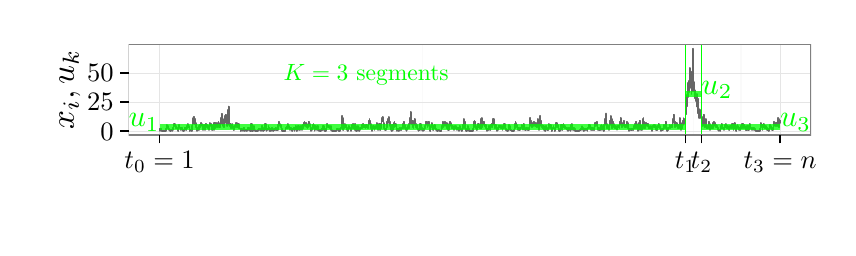
\begin{tikzpicture}[x=1pt,y=1pt]
\definecolor{fillColor}{RGB}{255,255,255}
\path[use as bounding box,fill=fillColor,fill opacity=0.00] (0,0) rectangle (289.08, 72.27);
\begin{scope}
\path[clip] (  0.00,  0.00) rectangle (289.08, 72.27);
\definecolor{drawColor}{RGB}{255,255,255}
\definecolor{fillColor}{RGB}{255,255,255}

\path[draw=drawColor,line width= 0.6pt,line join=round,line cap=round,fill=fillColor] (  0.00, -0.00) rectangle (289.08, 72.27);
\end{scope}
\begin{scope}
\path[clip] ( 36.46, 33.48) rectangle (283.08, 66.27);
\definecolor{fillColor}{RGB}{255,255,255}

\path[fill=fillColor] ( 36.46, 33.48) rectangle (283.08, 66.27);
\definecolor{drawColor}{gray}{0.98}

\path[draw=drawColor,line width= 0.6pt,line join=round] (142.71, 33.48) --
	(142.71, 66.27);

\path[draw=drawColor,line width= 0.6pt,line join=round] (240.61, 33.48) --
	(240.61, 66.27);

\path[draw=drawColor,line width= 0.6pt,line join=round] (257.67, 33.48) --
	(257.67, 66.27);
\definecolor{drawColor}{gray}{0.90}

\path[draw=drawColor,line width= 0.2pt,line join=round] ( 36.46, 34.97) --
	(283.08, 34.97);

\path[draw=drawColor,line width= 0.2pt,line join=round] ( 36.46, 45.46) --
	(283.08, 45.46);

\path[draw=drawColor,line width= 0.2pt,line join=round] ( 36.46, 55.96) --
	(283.08, 55.96);

\path[draw=drawColor,line width= 0.2pt,line join=round] ( 47.67, 33.48) --
	( 47.67, 66.27);

\path[draw=drawColor,line width= 0.2pt,line join=round] (237.74, 33.48) --
	(237.74, 66.27);

\path[draw=drawColor,line width= 0.2pt,line join=round] (243.48, 33.48) --
	(243.48, 66.27);

\path[draw=drawColor,line width= 0.2pt,line join=round] (271.87, 33.48) --
	(271.87, 66.27);
\definecolor{drawColor}{gray}{0.40}

\path[draw=drawColor,line width= 0.6pt,line join=round] ( 47.67, 35.39) --
	( 47.86, 35.39) --
	( 47.86, 34.97) --
	( 47.87, 34.97) --
	( 47.87, 35.39) --
	( 47.88, 35.39) --
	( 47.88, 35.81) --
	( 48.30, 35.81) --
	( 48.30, 35.39) --
	( 48.33, 35.39) --
	( 48.33, 34.97) --
	( 49.90, 34.97) --
	( 49.90, 35.39) --
	( 49.94, 35.39) --
	( 49.94, 35.81) --
	( 50.17, 35.81) --
	( 50.17, 36.23) --
	( 50.24, 36.23) --
	( 50.24, 36.65) --
	( 50.31, 36.65) --
	( 50.31, 37.07) --
	( 50.35, 37.07) --
	( 50.35, 36.65) --
	( 50.39, 36.65) --
	( 50.39, 36.23) --
	( 50.51, 36.23) --
	( 50.51, 36.65) --
	( 50.62, 36.65) --
	( 50.62, 36.23) --
	( 50.68, 36.23) --
	( 50.68, 36.65) --
	( 50.69, 36.65) --
	( 50.69, 36.23) --
	( 50.75, 36.23) --
	( 50.75, 35.81) --
	( 50.96, 35.81) --
	( 50.96, 35.39) --
	( 50.98, 35.39) --
	( 50.98, 35.81) --
	( 51.13, 35.81) --
	( 51.13, 35.39) --
	( 51.43, 35.39) --
	( 51.43, 34.97) --
	( 51.87, 34.97) --
	( 51.87, 35.39) --
	( 52.32, 35.39) --
	( 52.32, 34.97) --
	( 52.35, 34.97) --
	( 52.35, 35.39) --
	( 52.52, 35.39) --
	( 52.52, 35.81) --
	( 52.62, 35.81) --
	( 52.62, 36.23) --
	( 52.70, 36.23) --
	( 52.70, 36.65) --
	( 52.72, 36.65) --
	( 52.72, 37.07) --
	( 52.80, 37.07) --
	( 52.80, 36.65) --
	( 52.85, 36.65) --
	( 52.85, 37.07) --
	( 52.95, 37.07) --
	( 52.95, 37.49) --
	( 52.97, 37.49) --
	( 52.97, 37.07) --
	( 52.97, 37.07) --
	( 52.97, 37.49) --
	( 53.06, 37.49) --
	( 53.06, 37.07) --
	( 53.13, 37.07) --
	( 53.13, 37.49) --
	( 53.15, 37.49) --
	( 53.15, 37.07) --
	( 53.16, 37.07) --
	( 53.16, 36.65) --
	( 53.18, 36.65) --
	( 53.18, 37.07) --
	( 53.30, 37.07) --
	( 53.30, 36.65) --
	( 53.40, 36.65) --
	( 53.40, 36.23) --
	( 53.42, 36.23) --
	( 53.42, 35.81) --
	( 53.45, 35.81) --
	( 53.45, 36.23) --
	( 53.47, 36.23) --
	( 53.47, 36.65) --
	( 53.58, 36.65) --
	( 53.58, 36.23) --
	( 53.62, 36.23) --
	( 53.62, 35.81) --
	( 53.90, 35.81) --
	( 53.90, 36.23) --
	( 53.92, 36.23) --
	( 53.92, 35.81) --
	( 54.35, 35.81) --
	( 54.35, 34.97) --
	( 54.45, 34.97) --
	( 54.45, 35.39) --
	( 54.48, 35.39) --
	( 54.48, 35.81) --
	( 54.53, 35.81) --
	( 54.53, 36.23) --
	( 54.66, 36.23) --
	( 54.66, 36.65) --
	( 54.74, 36.65) --
	( 54.74, 37.07) --
	( 54.90, 37.07) --
	( 54.90, 36.65) --
	( 54.92, 36.65) --
	( 54.92, 36.23) --
	( 54.97, 36.23) --
	( 54.97, 35.81) --
	( 54.98, 35.81) --
	( 54.98, 36.23) --
	( 55.11, 36.23) --
	( 55.11, 35.81) --
	( 55.18, 35.81) --
	( 55.18, 35.39) --
	( 55.23, 35.39) --
	( 55.23, 35.81) --
	( 55.32, 35.81) --
	( 55.32, 36.23) --
	( 55.42, 36.23) --
	( 55.42, 35.81) --
	( 55.61, 35.81) --
	( 55.61, 36.23) --
	( 55.68, 36.23) --
	( 55.68, 35.81) --
	( 55.77, 35.81) --
	( 55.77, 35.39) --
	( 56.06, 35.39) --
	( 56.06, 34.97) --
	( 56.42, 34.97) --
	( 56.42, 35.39) --
	( 56.65, 35.39) --
	( 56.65, 35.81) --
	( 56.71, 35.81) --
	( 56.71, 36.23) --
	( 56.87, 36.23) --
	( 56.87, 35.81) --
	( 56.97, 35.81) --
	( 56.97, 36.23) --
	( 57.10, 36.23) --
	( 57.10, 35.81) --
	( 57.16, 35.81) --
	( 57.16, 35.39) --
	( 57.40, 35.39) --
	( 57.40, 35.81) --
	( 57.42, 35.81) --
	( 57.42, 35.39) --
	( 57.43, 35.39) --
	( 57.43, 35.81) --
	( 57.60, 35.81) --
	( 57.60, 36.65) --
	( 57.78, 36.65) --
	( 57.78, 37.07) --
	( 57.84, 37.07) --
	( 57.84, 36.65) --
	( 57.88, 36.65) --
	( 57.88, 36.23) --
	( 58.02, 36.23) --
	( 58.02, 37.07) --
	( 58.04, 37.07) --
	( 58.04, 37.49) --
	( 58.05, 37.49) --
	( 58.05, 36.65) --
	( 58.23, 36.65) --
	( 58.23, 36.23) --
	( 58.47, 36.23) --
	( 58.47, 35.39) --
	( 58.48, 35.39) --
	( 58.48, 34.97) --
	( 58.74, 34.97) --
	( 58.74, 35.39) --
	( 59.18, 35.39) --
	( 59.18, 34.97) --
	( 59.31, 34.97) --
	( 59.31, 35.39) --
	( 59.37, 35.39) --
	( 59.37, 35.81) --
	( 59.42, 35.81) --
	( 59.42, 36.65) --
	( 59.51, 36.65) --
	( 59.51, 37.49) --
	( 59.65, 37.49) --
	( 59.65, 37.91) --
	( 59.69, 37.91) --
	( 59.69, 38.33) --
	( 59.76, 38.33) --
	( 59.76, 37.91) --
	( 59.79, 37.91) --
	( 59.79, 39.17) --
	( 59.81, 39.17) --
	( 59.81, 39.59) --
	( 59.81, 39.59) --
	( 59.81, 39.17) --
	( 59.86, 39.17) --
	( 59.86, 40.01) --
	( 59.87, 40.01) --
	( 59.87, 39.17) --
	( 59.93, 39.17) --
	( 59.93, 39.59) --
	( 59.96, 39.59) --
	( 59.96, 38.75) --
	( 60.02, 38.75) --
	( 60.02, 39.17) --
	( 60.10, 39.17) --
	( 60.10, 38.75) --
	( 60.14, 38.75) --
	( 60.14, 38.33) --
	( 60.18, 38.33) --
	( 60.18, 39.59) --
	( 60.22, 39.59) --
	( 60.22, 40.01) --
	( 60.24, 40.01) --
	( 60.24, 39.59) --
	( 60.24, 39.59) --
	( 60.24, 38.75) --
	( 60.26, 38.75) --
	( 60.26, 38.33) --
	( 60.31, 38.33) --
	( 60.31, 37.49) --
	( 60.40, 37.49) --
	( 60.40, 37.91) --
	( 60.42, 37.91) --
	( 60.42, 38.33) --
	( 60.43, 38.33) --
	( 60.43, 38.75) --
	( 60.47, 38.75) --
	( 60.47, 38.33) --
	( 60.58, 38.33) --
	( 60.58, 38.75) --
	( 60.60, 38.75) --
	( 60.60, 39.17) --
	( 60.63, 39.17) --
	( 60.63, 37.91) --
	( 60.64, 37.91) --
	( 60.64, 38.33) --
	( 60.67, 38.33) --
	( 60.67, 37.91) --
	( 60.83, 37.91) --
	( 60.83, 37.49) --
	( 60.85, 37.49) --
	( 60.85, 37.07) --
	( 60.87, 37.07) --
	( 60.87, 36.23) --
	( 61.03, 36.23) --
	( 61.03, 35.39) --
	( 61.09, 35.39) --
	( 61.09, 34.97) --
	( 61.14, 34.97) --
	( 61.14, 35.39) --
	( 61.22, 35.39) --
	( 61.22, 35.81) --
	( 61.44, 35.81) --
	( 61.44, 36.23) --
	( 61.58, 36.23) --
	( 61.58, 35.81) --
	( 61.67, 35.81) --
	( 61.67, 35.39) --
	( 61.79, 35.39) --
	( 61.79, 35.81) --
	( 61.89, 35.81) --
	( 61.89, 35.39) --
	( 61.90, 35.39) --
	( 61.90, 35.81) --
	( 61.94, 35.81) --
	( 61.94, 36.23) --
	( 61.96, 36.23) --
	( 61.96, 36.65) --
	( 62.13, 36.65) --
	( 62.13, 37.07) --
	( 62.24, 37.07) --
	( 62.24, 36.65) --
	( 62.26, 36.65) --
	( 62.26, 37.07) --
	( 62.35, 37.07) --
	( 62.35, 36.65) --
	( 62.39, 36.65) --
	( 62.39, 36.23) --
	( 62.40, 36.23) --
	( 62.40, 37.07) --
	( 62.41, 37.07) --
	( 62.41, 36.65) --
	( 62.49, 36.65) --
	( 62.49, 37.07) --
	( 62.50, 37.07) --
	( 62.50, 37.49) --
	( 62.65, 37.49) --
	( 62.65, 37.91) --
	( 62.70, 37.91) --
	( 62.70, 37.49) --
	( 62.79, 37.49) --
	( 62.79, 37.91) --
	( 62.84, 37.91) --
	( 62.84, 37.07) --
	( 62.93, 37.07) --
	( 62.93, 37.49) --
	( 62.94, 37.49) --
	( 62.94, 37.07) --
	( 62.95, 37.07) --
	( 62.95, 36.65) --
	( 62.99, 36.65) --
	( 62.99, 37.49) --
	( 63.02, 37.49) --
	( 63.02, 37.07) --
	( 63.10, 37.07) --
	( 63.10, 36.65) --
	( 63.24, 36.65) --
	( 63.24, 36.23) --
	( 63.35, 36.23) --
	( 63.35, 36.65) --
	( 63.38, 36.65) --
	( 63.38, 36.23) --
	( 63.44, 36.23) --
	( 63.44, 35.39) --
	( 63.45, 35.39) --
	( 63.45, 35.81) --
	( 63.47, 35.81) --
	( 63.47, 36.23) --
	( 63.52, 36.23) --
	( 63.52, 36.65) --
	( 63.77, 36.65) --
	( 63.77, 37.07) --
	( 63.79, 37.07) --
	( 63.79, 36.65) --
	( 63.90, 36.65) --
	( 63.90, 36.23) --
	( 63.92, 36.23) --
	( 63.92, 35.81) --
	( 63.97, 35.81) --
	( 63.97, 35.39) --
	( 64.05, 35.39) --
	( 64.05, 35.81) --
	( 64.16, 35.81) --
	( 64.16, 36.23) --
	( 64.18, 36.23) --
	( 64.18, 36.65) --
	( 64.19, 36.65) --
	( 64.19, 37.07) --
	( 64.22, 37.07) --
	( 64.22, 36.65) --
	( 64.23, 36.65) --
	( 64.23, 37.07) --
	( 64.30, 37.07) --
	( 64.30, 37.49) --
	( 64.50, 37.49) --
	( 64.50, 37.07) --
	( 64.58, 37.07) --
	( 64.58, 37.49) --
	( 64.63, 37.49) --
	( 64.63, 37.07) --
	( 64.64, 37.07) --
	( 64.64, 36.65) --
	( 64.65, 36.65) --
	( 64.65, 37.07) --
	( 64.68, 37.07) --
	( 64.68, 36.65) --
	( 64.74, 36.65) --
	( 64.74, 36.23) --
	( 64.96, 36.23) --
	( 64.96, 36.65) --
	( 65.00, 36.65) --
	( 65.00, 37.07) --
	( 65.03, 37.07) --
	( 65.03, 36.65) --
	( 65.05, 36.65) --
	( 65.05, 36.23) --
	( 65.09, 36.23) --
	( 65.09, 35.81) --
	( 65.39, 35.81) --
	( 65.39, 36.23) --
	( 65.41, 36.23) --
	( 65.41, 35.81) --
	( 65.44, 35.81) --
	( 65.44, 35.39) --
	( 65.50, 35.39) --
	( 65.50, 35.81) --
	( 65.51, 35.81) --
	( 65.51, 36.23) --
	( 65.60, 36.23) --
	( 65.60, 36.65) --
	( 65.68, 36.65) --
	( 65.68, 37.07) --
	( 65.70, 37.07) --
	( 65.70, 37.49) --
	( 65.79, 37.49) --
	( 65.79, 37.91) --
	( 65.84, 37.91) --
	( 65.84, 37.49) --
	( 65.93, 37.49) --
	( 65.93, 37.91) --
	( 65.94, 37.91) --
	( 65.94, 37.49) --
	( 65.95, 37.49) --
	( 65.95, 37.07) --
	( 66.01, 37.07) --
	( 66.01, 36.65) --
	( 66.05, 36.65) --
	( 66.05, 37.07) --
	( 66.12, 37.07) --
	( 66.12, 37.49) --
	( 66.13, 37.49) --
	( 66.13, 37.07) --
	( 66.13, 37.07) --
	( 66.13, 37.49) --
	( 66.15, 37.49) --
	( 66.15, 37.07) --
	( 66.18, 37.07) --
	( 66.18, 37.49) --
	( 66.24, 37.49) --
	( 66.24, 37.07) --
	( 66.30, 37.07) --
	( 66.30, 37.49) --
	( 66.38, 37.49) --
	( 66.38, 37.07) --
	( 66.50, 37.07) --
	( 66.50, 36.65) --
	( 66.57, 36.65) --
	( 66.57, 36.23) --
	( 66.58, 36.23) --
	( 66.58, 35.81) --
	( 66.63, 35.81) --
	( 66.63, 35.39) --
	( 66.65, 35.39) --
	( 66.65, 35.81) --
	( 66.67, 35.81) --
	( 66.67, 35.39) --
	( 66.81, 35.39) --
	( 66.81, 35.81) --
	( 67.05, 35.81) --
	( 67.05, 36.23) --
	( 67.10, 36.23) --
	( 67.10, 35.81) --
	( 67.26, 35.81) --
	( 67.26, 35.39) --
	( 67.28, 35.39) --
	( 67.28, 36.23) --
	( 67.30, 36.23) --
	( 67.30, 36.65) --
	( 67.32, 36.65) --
	( 67.32, 37.07) --
	( 67.34, 37.07) --
	( 67.34, 37.49) --
	( 67.38, 37.49) --
	( 67.38, 37.91) --
	( 67.50, 37.91) --
	( 67.50, 37.49) --
	( 67.57, 37.49) --
	( 67.57, 37.91) --
	( 67.73, 37.91) --
	( 67.73, 37.07) --
	( 67.75, 37.07) --
	( 67.75, 36.65) --
	( 67.76, 36.65) --
	( 67.76, 36.23) --
	( 67.82, 36.23) --
	( 67.82, 35.81) --
	( 67.91, 35.81) --
	( 67.91, 36.23) --
	( 67.93, 36.23) --
	( 67.93, 37.07) --
	( 68.05, 37.07) --
	( 68.05, 37.49) --
	( 68.09, 37.49) --
	( 68.09, 37.91) --
	( 68.24, 37.91) --
	( 68.24, 37.49) --
	( 68.35, 37.49) --
	( 68.35, 37.07) --
	( 68.38, 37.07) --
	( 68.38, 36.23) --
	( 68.40, 36.23) --
	( 68.40, 36.65) --
	( 68.47, 36.65) --
	( 68.47, 36.23) --
	( 68.49, 36.23) --
	( 68.49, 36.65) --
	( 68.50, 36.65) --
	( 68.50, 36.23) --
	( 68.53, 36.23) --
	( 68.53, 36.65) --
	( 68.54, 36.65) --
	( 68.54, 36.23) --
	( 68.60, 36.23) --
	( 68.60, 36.65) --
	( 68.67, 36.65) --
	( 68.67, 37.07) --
	( 68.70, 37.07) --
	( 68.70, 37.49) --
	( 68.78, 37.49) --
	( 68.78, 37.91) --
	( 68.85, 37.91) --
	( 68.85, 37.49) --
	( 68.85, 37.49) --
	( 68.85, 37.91) --
	( 68.94, 37.91) --
	( 68.94, 37.49) --
	( 68.97, 37.49) --
	( 68.97, 37.91) --
	( 68.97, 37.91) --
	( 68.97, 38.33) --
	( 68.98, 38.33) --
	( 68.98, 37.91) --
	( 69.04, 37.91) --
	( 69.04, 37.49) --
	( 69.12, 37.49) --
	( 69.12, 37.07) --
	( 69.15, 37.07) --
	( 69.15, 36.65) --
	( 69.22, 36.65) --
	( 69.22, 36.23) --
	( 69.23, 36.23) --
	( 69.23, 36.65) --
	( 69.26, 36.65) --
	( 69.26, 37.49) --
	( 69.30, 37.49) --
	( 69.30, 37.07) --
	( 69.42, 37.07) --
	( 69.42, 36.65) --
	( 69.42, 36.65) --
	( 69.42, 36.23) --
	( 69.44, 36.23) --
	( 69.44, 36.65) --
	( 69.49, 36.65) --
	( 69.49, 37.07) --
	( 69.56, 37.07) --
	( 69.56, 37.49) --
	( 69.66, 37.49) --
	( 69.66, 37.91) --
	( 69.68, 37.91) --
	( 69.68, 37.49) --
	( 69.69, 37.49) --
	( 69.69, 37.91) --
	( 69.70, 37.91) --
	( 69.70, 38.33) --
	( 69.71, 38.33) --
	( 69.71, 37.91) --
	( 69.71, 37.91) --
	( 69.71, 37.49) --
	( 69.74, 37.49) --
	( 69.74, 37.91) --
	( 69.88, 37.91) --
	( 69.88, 38.33) --
	( 69.89, 38.33) --
	( 69.89, 37.91) --
	( 69.93, 37.91) --
	( 69.93, 38.33) --
	( 69.94, 38.33) --
	( 69.94, 37.91) --
	( 69.96, 37.91) --
	( 69.96, 39.17) --
	( 69.96, 39.17) --
	( 69.96, 39.59) --
	( 69.99, 39.59) --
	( 69.99, 39.17) --
	( 70.01, 39.17) --
	( 70.01, 39.59) --
	( 70.05, 39.59) --
	( 70.05, 40.01) --
	( 70.09, 40.01) --
	( 70.09, 40.43) --
	( 70.11, 40.43) --
	( 70.11, 40.01) --
	( 70.14, 40.01) --
	( 70.14, 39.59) --
	( 70.15, 39.59) --
	( 70.15, 39.17) --
	( 70.16, 39.17) --
	( 70.16, 39.59) --
	( 70.18, 39.59) --
	( 70.18, 40.01) --
	( 70.19, 40.01) --
	( 70.19, 39.59) --
	( 70.20, 39.59) --
	( 70.20, 40.43) --
	( 70.26, 40.43) --
	( 70.26, 40.85) --
	( 70.32, 40.85) --
	( 70.32, 41.27) --
	( 70.33, 41.27) --
	( 70.33, 40.85) --
	( 70.38, 40.85) --
	( 70.38, 40.43) --
	( 70.41, 40.43) --
	( 70.41, 39.17) --
	( 70.41, 39.17) --
	( 70.41, 38.33) --
	( 70.43, 38.33) --
	( 70.43, 38.75) --
	( 70.48, 38.75) --
	( 70.48, 39.17) --
	( 70.50, 39.17) --
	( 70.50, 38.75) --
	( 70.54, 38.75) --
	( 70.54, 38.33) --
	( 70.56, 38.33) --
	( 70.56, 37.91) --
	( 70.63, 37.91) --
	( 70.63, 37.49) --
	( 70.65, 37.49) --
	( 70.65, 36.65) --
	( 70.69, 36.65) --
	( 70.69, 37.07) --
	( 70.70, 37.07) --
	( 70.70, 36.23) --
	( 70.79, 36.23) --
	( 70.79, 36.65) --
	( 70.87, 36.65) --
	( 70.87, 37.07) --
	( 70.87, 37.07) --
	( 70.87, 36.65) --
	( 70.93, 36.65) --
	( 70.93, 36.23) --
	( 71.00, 36.23) --
	( 71.00, 37.07) --
	( 71.04, 37.07) --
	( 71.04, 37.49) --
	( 71.08, 37.49) --
	( 71.08, 37.91) --
	( 71.08, 37.91) --
	( 71.08, 37.49) --
	( 71.15, 37.49) --
	( 71.15, 37.91) --
	( 71.17, 37.91) --
	( 71.17, 38.33) --
	( 71.24, 38.33) --
	( 71.24, 37.91) --
	( 71.27, 37.91) --
	( 71.27, 38.33) --
	( 71.27, 38.33) --
	( 71.27, 38.75) --
	( 71.31, 38.75) --
	( 71.31, 39.17) --
	( 71.33, 39.17) --
	( 71.33, 38.75) --
	( 71.35, 38.75) --
	( 71.35, 39.17) --
	( 71.39, 39.17) --
	( 71.39, 39.59) --
	( 71.40, 39.59) --
	( 71.40, 40.01) --
	( 71.41, 40.01) --
	( 71.41, 40.43) --
	( 71.46, 40.43) --
	( 71.46, 40.85) --
	( 71.48, 40.85) --
	( 71.48, 40.43) --
	( 71.51, 40.43) --
	( 71.51, 40.85) --
	( 71.52, 40.85) --
	( 71.52, 40.43) --
	( 71.53, 40.43) --
	( 71.53, 40.01) --
	( 71.56, 40.01) --
	( 71.56, 40.43) --
	( 71.57, 40.43) --
	( 71.57, 40.85) --
	( 71.60, 40.85) --
	( 71.60, 40.43) --
	( 71.67, 40.43) --
	( 71.67, 40.85) --
	( 71.72, 40.85) --
	( 71.72, 40.43) --
	( 71.75, 40.43) --
	( 71.75, 40.01) --
	( 71.76, 40.01) --
	( 71.76, 40.43) --
	( 71.77, 40.43) --
	( 71.77, 40.01) --
	( 71.80, 40.01) --
	( 71.80, 40.43) --
	( 71.83, 40.43) --
	( 71.83, 40.01) --
	( 71.85, 40.01) --
	( 71.85, 39.59) --
	( 71.86, 39.59) --
	( 71.86, 39.17) --
	( 71.89, 39.17) --
	( 71.89, 38.75) --
	( 71.91, 38.75) --
	( 71.91, 38.33) --
	( 71.95, 38.33) --
	( 71.95, 37.91) --
	( 72.00, 37.91) --
	( 72.00, 37.49) --
	( 72.00, 37.49) --
	( 72.00, 37.91) --
	( 72.01, 37.91) --
	( 72.01, 37.49) --
	( 72.02, 37.49) --
	( 72.02, 37.07) --
	( 72.07, 37.07) --
	( 72.07, 36.65) --
	( 72.08, 36.65) --
	( 72.08, 37.07) --
	( 72.11, 37.07) --
	( 72.11, 37.49) --
	( 72.12, 37.49) --
	( 72.12, 37.07) --
	( 72.19, 37.07) --
	( 72.19, 37.49) --
	( 72.21, 37.49) --
	( 72.21, 37.07) --
	( 72.25, 37.07) --
	( 72.25, 36.65) --
	( 72.26, 36.65) --
	( 72.26, 37.07) --
	( 72.27, 37.07) --
	( 72.27, 37.91) --
	( 72.28, 37.91) --
	( 72.28, 38.33) --
	( 72.34, 38.33) --
	( 72.34, 38.75) --
	( 72.37, 38.75) --
	( 72.37, 39.17) --
	( 72.38, 39.17) --
	( 72.38, 39.59) --
	( 72.39, 39.59) --
	( 72.39, 40.01) --
	( 72.43, 40.01) --
	( 72.43, 40.43) --
	( 72.44, 40.43) --
	( 72.44, 40.85) --
	( 72.45, 40.85) --
	( 72.45, 40.43) --
	( 72.46, 40.43) --
	( 72.46, 40.85) --
	( 72.47, 40.85) --
	( 72.47, 42.11) --
	( 72.49, 42.11) --
	( 72.49, 42.53) --
	( 72.51, 42.53) --
	( 72.51, 42.11) --
	( 72.52, 42.11) --
	( 72.52, 42.53) --
	( 72.53, 42.53) --
	( 72.53, 42.94) --
	( 72.55, 42.94) --
	( 72.55, 43.36) --
	( 72.56, 43.36) --
	( 72.56, 43.78) --
	( 72.56, 43.78) --
	( 72.56, 43.36) --
	( 72.61, 43.36) --
	( 72.61, 43.78) --
	( 72.64, 43.78) --
	( 72.64, 43.36) --
	( 72.71, 43.36) --
	( 72.71, 42.94) --
	( 72.72, 42.94) --
	( 72.72, 42.53) --
	( 72.73, 42.53) --
	( 72.73, 42.11) --
	( 72.78, 42.11) --
	( 72.78, 41.69) --
	( 72.82, 41.69) --
	( 72.82, 41.27) --
	( 72.83, 41.27) --
	( 72.83, 40.85) --
	( 72.83, 40.85) --
	( 72.83, 40.43) --
	( 72.87, 40.43) --
	( 72.87, 40.01) --
	( 72.89, 40.01) --
	( 72.89, 39.59) --
	( 72.91, 39.59) --
	( 72.91, 39.17) --
	( 72.92, 39.17) --
	( 72.92, 37.91) --
	( 72.93, 37.91) --
	( 72.93, 38.33) --
	( 72.94, 38.33) --
	( 72.94, 37.49) --
	( 72.97, 37.49) --
	( 72.97, 37.07) --
	( 72.98, 37.07) --
	( 72.98, 36.65) --
	( 72.99, 36.65) --
	( 72.99, 37.07) --
	( 72.99, 37.07) --
	( 72.99, 37.49) --
	( 73.01, 37.49) --
	( 73.01, 37.07) --
	( 73.06, 37.07) --
	( 73.06, 36.65) --
	( 73.18, 36.65) --
	( 73.18, 37.49) --
	( 73.38, 37.49) --
	( 73.38, 37.07) --
	( 73.44, 37.07) --
	( 73.44, 35.81) --
	( 73.60, 35.81) --
	( 73.60, 36.65) --
	( 73.63, 36.65) --
	( 73.63, 35.81) --
	( 73.71, 35.81) --
	( 73.71, 36.23) --
	( 73.84, 36.23) --
	( 73.84, 36.65) --
	( 73.98, 36.65) --
	( 73.98, 37.07) --
	( 73.99, 37.07) --
	( 73.99, 37.49) --
	( 74.05, 37.49) --
	( 74.05, 36.65) --
	( 74.15, 36.65) --
	( 74.15, 36.23) --
	( 74.29, 36.23) --
	( 74.29, 35.81) --
	( 74.30, 35.81) --
	( 74.30, 36.23) --
	( 74.43, 36.23) --
	( 74.43, 35.81) --
	( 74.43, 35.81) --
	( 74.43, 35.39) --
	( 74.46, 35.39) --
	( 74.46, 35.81) --
	( 74.46, 35.81) --
	( 74.46, 36.23) --
	( 74.73, 36.23) --
	( 74.73, 36.65) --
	( 74.74, 36.65) --
	( 74.74, 36.23) --
	( 74.88, 36.23) --
	( 74.88, 36.65) --
	( 74.91, 36.65) --
	( 74.91, 36.23) --
	( 74.98, 36.23) --
	( 74.98, 36.65) --
	( 75.11, 36.65) --
	( 75.11, 37.07) --
	( 75.18, 37.07) --
	( 75.18, 36.65) --
	( 75.22, 36.65) --
	( 75.22, 37.07) --
	( 75.28, 37.07) --
	( 75.28, 37.91) --
	( 75.33, 37.91) --
	( 75.33, 37.49) --
	( 75.35, 37.49) --
	( 75.35, 37.07) --
	( 75.43, 37.07) --
	( 75.43, 36.65) --
	( 75.48, 36.65) --
	( 75.48, 37.07) --
	( 75.49, 37.07) --
	( 75.49, 37.49) --
	( 75.56, 37.49) --
	( 75.56, 37.07) --
	( 75.60, 37.07) --
	( 75.60, 37.49) --
	( 75.64, 37.49) --
	( 75.64, 37.91) --
	( 75.65, 37.91) --
	( 75.65, 37.49) --
	( 75.66, 37.49) --
	( 75.66, 37.07) --
	( 75.69, 37.07) --
	( 75.69, 36.65) --
	( 75.72, 36.65) --
	( 75.72, 36.23) --
	( 75.80, 36.23) --
	( 75.80, 36.65) --
	( 75.82, 36.65) --
	( 75.82, 37.07) --
	( 75.86, 37.07) --
	( 75.86, 36.65) --
	( 75.94, 36.65) --
	( 75.94, 36.23) --
	( 75.96, 36.23) --
	( 75.96, 36.65) --
	( 75.96, 36.65) --
	( 75.96, 37.07) --
	( 76.06, 37.07) --
	( 76.06, 37.49) --
	( 76.09, 37.49) --
	( 76.09, 37.07) --
	( 76.09, 37.07) --
	( 76.09, 37.49) --
	( 76.25, 37.49) --
	( 76.25, 37.07) --
	( 76.27, 37.07) --
	( 76.27, 36.65) --
	( 76.40, 36.65) --
	( 76.40, 35.81) --
	( 76.48, 35.81) --
	( 76.48, 36.23) --
	( 76.51, 36.23) --
	( 76.51, 35.81) --
	( 76.51, 35.81) --
	( 76.51, 36.23) --
	( 76.54, 36.23) --
	( 76.54, 35.81) --
	( 76.93, 35.81) --
	( 76.93, 35.39) --
	( 76.96, 35.39) --
	( 76.96, 34.97) --
	( 77.15, 34.97) --
	( 77.15, 35.39) --
	( 77.26, 35.39) --
	( 77.26, 35.81) --
	( 77.55, 35.81) --
	( 77.55, 35.39) --
	( 77.71, 35.39) --
	( 77.71, 34.97) --
	( 77.90, 34.97) --
	( 77.90, 35.39) --
	( 77.95, 35.39) --
	( 77.95, 35.81) --
	( 77.96, 35.81) --
	( 77.96, 36.23) --
	( 78.34, 36.23) --
	( 78.34, 35.81) --
	( 78.40, 35.81) --
	( 78.40, 35.39) --
	( 78.41, 35.39) --
	( 78.41, 34.97) --
	( 78.64, 34.97) --
	( 78.64, 35.39) --
	( 79.09, 35.39) --
	( 79.09, 34.97) --
	( 79.30, 34.97) --
	( 79.30, 35.39) --
	( 79.43, 35.39) --
	( 79.43, 35.81) --
	( 79.60, 35.81) --
	( 79.60, 36.23) --
	( 79.64, 36.23) --
	( 79.64, 35.81) --
	( 79.75, 35.81) --
	( 79.75, 35.39) --
	( 79.92, 35.39) --
	( 79.92, 35.81) --
	( 79.97, 35.81) --
	( 79.97, 36.23) --
	( 80.05, 36.23) --
	( 80.05, 35.81) --
	( 80.36, 35.81) --
	( 80.36, 35.39) --
	( 80.42, 35.39) --
	( 80.42, 34.97) --
	( 80.60, 34.97) --
	( 80.60, 36.23) --
	( 80.63, 36.23) --
	( 80.63, 37.49) --
	( 81.04, 37.49) --
	( 81.04, 36.23) --
	( 81.07, 36.23) --
	( 81.07, 35.81) --
	( 81.07, 35.81) --
	( 81.07, 34.97) --
	( 81.32, 34.97) --
	( 81.32, 35.39) --
	( 81.35, 35.39) --
	( 81.35, 35.81) --
	( 81.53, 35.81) --
	( 81.53, 36.23) --
	( 81.68, 36.23) --
	( 81.68, 36.65) --
	( 81.73, 36.65) --
	( 81.73, 36.23) --
	( 81.80, 36.23) --
	( 81.80, 35.81) --
	( 81.98, 35.81) --
	( 81.98, 35.39) --
	( 82.12, 35.39) --
	( 82.12, 34.97) --
	( 83.16, 34.97) --
	( 83.16, 35.39) --
	( 83.40, 35.39) --
	( 83.40, 35.81) --
	( 83.61, 35.81) --
	( 83.61, 35.39) --
	( 83.64, 35.39) --
	( 83.64, 35.81) --
	( 83.85, 35.81) --
	( 83.85, 35.39) --
	( 83.90, 35.39) --
	( 83.90, 35.81) --
	( 84.08, 35.81) --
	( 84.08, 35.39) --
	( 84.34, 35.39) --
	( 84.34, 34.97) --
	( 84.38, 34.97) --
	( 84.38, 35.39) --
	( 84.61, 35.39) --
	( 84.61, 35.81) --
	( 84.63, 35.81) --
	( 84.63, 36.23) --
	( 84.65, 36.23) --
	( 84.65, 36.65) --
	( 84.83, 36.65) --
	( 84.83, 36.23) --
	( 85.06, 36.23) --
	( 85.06, 35.81) --
	( 85.08, 35.81) --
	( 85.08, 35.39) --
	( 85.10, 35.39) --
	( 85.10, 34.97) --
	( 85.20, 34.97) --
	( 85.20, 35.39) --
	( 85.58, 35.39) --
	( 85.58, 35.81) --
	( 85.65, 35.81) --
	( 85.65, 35.39) --
	( 85.73, 35.39) --
	( 85.73, 35.81) --
	( 85.81, 35.81) --
	( 85.81, 36.23) --
	( 85.84, 36.23) --
	( 85.84, 37.07) --
	( 85.85, 37.07) --
	( 85.85, 37.49) --
	( 86.02, 37.49) --
	( 86.02, 37.07) --
	( 86.17, 37.07) --
	( 86.17, 36.65) --
	( 86.25, 36.65) --
	( 86.25, 36.23) --
	( 86.29, 36.23) --
	( 86.29, 35.39) --
	( 86.30, 35.39) --
	( 86.30, 34.97) --
	( 86.33, 34.97) --
	( 86.33, 35.39) --
	( 86.56, 35.39) --
	( 86.56, 35.81) --
	( 86.78, 35.81) --
	( 86.78, 35.39) --
	( 86.91, 35.39) --
	( 86.91, 35.81) --
	( 86.97, 35.81) --
	( 86.97, 36.65) --
	( 87.01, 36.65) --
	( 87.01, 36.23) --
	( 87.36, 36.23) --
	( 87.36, 35.81) --
	( 87.41, 35.81) --
	( 87.41, 34.97) --
	( 87.47, 34.97) --
	( 87.47, 35.39) --
	( 87.71, 35.39) --
	( 87.71, 35.81) --
	( 87.92, 35.81) --
	( 87.92, 34.97) --
	( 87.98, 34.97) --
	( 87.98, 35.39) --
	( 88.13, 35.39) --
	( 88.13, 35.81) --
	( 88.38, 35.81) --
	( 88.38, 36.23) --
	( 88.41, 36.23) --
	( 88.41, 35.81) --
	( 88.57, 35.81) --
	( 88.57, 34.97) --
	( 88.82, 34.97) --
	( 88.82, 35.39) --
	( 89.25, 35.39) --
	( 89.25, 35.81) --
	( 89.27, 35.81) --
	( 89.27, 35.39) --
	( 89.35, 35.39) --
	( 89.35, 35.81) --
	( 89.51, 35.81) --
	( 89.51, 36.23) --
	( 89.69, 36.23) --
	( 89.69, 35.81) --
	( 89.80, 35.81) --
	( 89.80, 35.39) --
	( 89.81, 35.39) --
	( 89.81, 35.81) --
	( 89.94, 35.81) --
	( 89.94, 35.39) --
	( 90.07, 35.39) --
	( 90.07, 35.81) --
	( 90.26, 35.81) --
	( 90.26, 35.39) --
	( 90.41, 35.39) --
	( 90.41, 35.81) --
	( 90.43, 35.81) --
	( 90.43, 36.23) --
	( 90.48, 36.23) --
	( 90.48, 37.07) --
	( 90.52, 37.07) --
	( 90.52, 36.65) --
	( 90.55, 36.65) --
	( 90.55, 37.07) --
	( 90.59, 37.07) --
	( 90.59, 37.49) --
	( 90.69, 37.49) --
	( 90.69, 37.91) --
	( 90.80, 37.91) --
	( 90.80, 38.33) --
	( 90.86, 38.33) --
	( 90.86, 37.91) --
	( 90.87, 37.91) --
	( 90.87, 38.33) --
	( 90.88, 38.33) --
	( 90.88, 37.91) --
	( 90.93, 37.91) --
	( 90.93, 37.07) --
	( 90.99, 37.07) --
	( 90.99, 37.49) --
	( 91.00, 37.49) --
	( 91.00, 37.07) --
	( 91.01, 37.07) --
	( 91.01, 37.49) --
	( 91.03, 37.49) --
	( 91.03, 37.07) --
	( 91.11, 37.07) --
	( 91.11, 37.49) --
	( 91.14, 37.49) --
	( 91.14, 37.07) --
	( 91.25, 37.07) --
	( 91.25, 36.65) --
	( 91.28, 36.65) --
	( 91.28, 37.07) --
	( 91.32, 37.07) --
	( 91.32, 36.65) --
	( 91.38, 36.65) --
	( 91.38, 37.07) --
	( 91.44, 37.07) --
	( 91.44, 36.65) --
	( 91.45, 36.65) --
	( 91.45, 36.23) --
	( 91.52, 36.23) --
	( 91.52, 36.65) --
	( 91.56, 36.65) --
	( 91.56, 36.23) --
	( 91.73, 36.23) --
	( 91.73, 35.81) --
	( 91.83, 35.81) --
	( 91.83, 35.39) --
	( 91.97, 35.39) --
	( 91.97, 34.97) --
	( 93.19, 34.97) --
	( 93.19, 35.39) --
	( 93.21, 35.39) --
	( 93.21, 35.81) --
	( 93.35, 35.81) --
	( 93.35, 36.23) --
	( 93.63, 36.23) --
	( 93.63, 35.81) --
	( 93.63, 35.81) --
	( 93.63, 36.23) --
	( 93.66, 36.23) --
	( 93.66, 36.65) --
	( 93.66, 36.65) --
	( 93.66, 36.23) --
	( 93.80, 36.23) --
	( 93.80, 35.81) --
	( 93.89, 35.81) --
	( 93.89, 36.23) --
	( 93.96, 36.23) --
	( 93.96, 36.65) --
	( 94.06, 36.65) --
	( 94.06, 37.49) --
	( 94.08, 37.49) --
	( 94.08, 37.07) --
	( 94.10, 37.07) --
	( 94.10, 36.65) --
	( 94.33, 36.65) --
	( 94.33, 36.23) --
	( 94.37, 36.23) --
	( 94.37, 36.65) --
	( 94.41, 36.65) --
	( 94.41, 36.23) --
	( 94.43, 36.23) --
	( 94.43, 36.65) --
	( 94.51, 36.65) --
	( 94.51, 35.81) --
	( 94.78, 35.81) --
	( 94.78, 36.23) --
	( 94.82, 36.23) --
	( 94.82, 35.81) --
	( 94.88, 35.81) --
	( 94.88, 35.39) --
	( 94.90, 35.39) --
	( 94.90, 35.81) --
	( 94.98, 35.81) --
	( 94.98, 36.23) --
	( 95.23, 36.23) --
	( 95.23, 35.81) --
	( 95.35, 35.81) --
	( 95.35, 35.39) --
	( 95.43, 35.39) --
	( 95.43, 34.97) --
	( 95.67, 34.97) --
	( 95.67, 35.39) --
	( 95.68, 35.39) --
	( 95.68, 35.81) --
	( 96.00, 35.81) --
	( 96.00, 36.23) --
	( 96.12, 36.23) --
	( 96.12, 35.39) --
	( 96.45, 35.39) --
	( 96.45, 34.97) --
	( 96.46, 34.97) --
	( 96.46, 35.39) --
	( 96.64, 35.39) --
	( 96.64, 35.81) --
	( 96.71, 35.81) --
	( 96.71, 36.23) --
	( 96.74, 36.23) --
	( 96.74, 36.65) --
	( 96.91, 36.65) --
	( 96.91, 36.23) --
	( 97.09, 36.23) --
	( 97.09, 35.81) --
	( 97.16, 35.81) --
	( 97.16, 35.39) --
	( 97.19, 35.39) --
	( 97.19, 34.97) --
	( 97.24, 34.97) --
	( 97.24, 35.39) --
	( 97.61, 35.39) --
	( 97.61, 35.81) --
	( 97.68, 35.81) --
	( 97.68, 36.23) --
	( 97.69, 36.23) --
	( 97.69, 35.81) --
	( 97.69, 35.81) --
	( 97.69, 36.23) --
	( 97.80, 36.23) --
	( 97.80, 36.65) --
	( 98.06, 36.65) --
	( 98.06, 36.23) --
	( 98.08, 36.23) --
	( 98.08, 36.65) --
	( 98.13, 36.65) --
	( 98.13, 36.23) --
	( 98.14, 36.23) --
	( 98.14, 35.81) --
	( 98.24, 35.81) --
	( 98.24, 35.39) --
	( 98.37, 35.39) --
	( 98.37, 35.81) --
	( 98.45, 35.81) --
	( 98.45, 36.23) --
	( 98.53, 36.23) --
	( 98.53, 35.81) --
	( 98.58, 35.81) --
	( 98.58, 36.23) --
	( 98.67, 36.23) --
	( 98.67, 36.65) --
	( 98.81, 36.65) --
	( 98.81, 36.23) --
	( 98.83, 36.23) --
	( 98.83, 36.65) --
	( 98.90, 36.65) --
	( 98.90, 36.23) --
	( 99.03, 36.23) --
	( 99.03, 35.81) --
	( 99.12, 35.81) --
	( 99.12, 35.39) --
	( 99.14, 35.39) --
	( 99.14, 35.81) --
	( 99.17, 35.81) --
	( 99.17, 36.23) --
	( 99.28, 36.23) --
	( 99.28, 35.81) --
	( 99.33, 35.81) --
	( 99.33, 36.23) --
	( 99.41, 36.23) --
	( 99.41, 35.81) --
	( 99.43, 35.81) --
	( 99.43, 36.23) --
	( 99.54, 36.23) --
	( 99.54, 36.65) --
	( 99.58, 36.65) --
	( 99.58, 37.07) --
	( 99.64, 37.07) --
	( 99.64, 37.49) --
	( 99.72, 37.49) --
	( 99.72, 37.91) --
	( 99.78, 37.91) --
	( 99.78, 37.49) --
	( 99.87, 37.49) --
	( 99.87, 37.07) --
	( 99.92, 37.07) --
	( 99.92, 37.49) --
	( 99.92, 37.49) --
	( 99.92, 37.91) --
	( 99.98, 37.91) --
	( 99.98, 38.33) --
	( 99.99, 38.33) --
	( 99.99, 37.91) --
	(100.02, 37.91) --
	(100.02, 37.49) --
	(100.05, 37.49) --
	(100.05, 37.91) --
	(100.07, 37.91) --
	(100.07, 37.07) --
	(100.17, 37.07) --
	(100.17, 36.65) --
	(100.18, 36.65) --
	(100.18, 37.07) --
	(100.33, 37.07) --
	(100.33, 37.49) --
	(100.36, 37.49) --
	(100.36, 37.07) --
	(100.37, 37.07) --
	(100.37, 36.65) --
	(100.37, 36.65) --
	(100.37, 37.07) --
	(100.40, 37.07) --
	(100.40, 37.49) --
	(100.42, 37.49) --
	(100.42, 37.91) --
	(100.43, 37.91) --
	(100.43, 37.49) --
	(100.46, 37.49) --
	(100.46, 37.91) --
	(100.50, 37.91) --
	(100.50, 37.49) --
	(100.60, 37.49) --
	(100.60, 37.91) --
	(100.62, 37.91) --
	(100.62, 37.49) --
	(100.71, 37.49) --
	(100.71, 37.91) --
	(100.78, 37.91) --
	(100.78, 37.49) --
	(100.82, 37.49) --
	(100.82, 37.07) --
	(100.85, 37.07) --
	(100.85, 36.65) --
	(100.86, 36.65) --
	(100.86, 37.07) --
	(100.91, 37.07) --
	(100.91, 36.65) --
	(101.05, 36.65) --
	(101.05, 36.23) --
	(101.06, 36.23) --
	(101.06, 35.81) --
	(101.09, 35.81) --
	(101.09, 36.23) --
	(101.10, 36.23) --
	(101.10, 36.65) --
	(101.31, 36.65) --
	(101.31, 36.23) --
	(101.38, 36.23) --
	(101.38, 36.65) --
	(101.44, 36.65) --
	(101.44, 37.07) --
	(101.46, 37.07) --
	(101.46, 37.49) --
	(101.52, 37.49) --
	(101.52, 38.33) --
	(101.54, 38.33) --
	(101.54, 37.91) --
	(101.54, 37.91) --
	(101.54, 37.49) --
	(101.58, 37.49) --
	(101.58, 37.91) --
	(101.60, 37.91) --
	(101.60, 37.49) --
	(101.69, 37.49) --
	(101.69, 37.91) --
	(101.83, 37.91) --
	(101.83, 37.49) --
	(101.88, 37.49) --
	(101.88, 37.07) --
	(101.91, 37.07) --
	(101.91, 36.65) --
	(101.93, 36.65) --
	(101.93, 37.49) --
	(101.97, 37.49) --
	(101.97, 37.07) --
	(101.97, 37.07) --
	(101.97, 36.65) --
	(101.97, 36.65) --
	(101.97, 37.07) --
	(102.02, 37.07) --
	(102.02, 36.65) --
	(102.14, 36.65) --
	(102.14, 36.23) --
	(102.38, 36.23) --
	(102.38, 35.39) --
	(102.42, 35.39) --
	(102.42, 34.97) --
	(102.49, 34.97) --
	(102.49, 35.39) --
	(102.71, 35.39) --
	(102.71, 35.81) --
	(102.87, 35.81) --
	(102.87, 36.23) --
	(102.93, 36.23) --
	(102.93, 35.81) --
	(103.11, 35.81) --
	(103.11, 36.65) --
	(103.16, 36.65) --
	(103.16, 36.23) --
	(103.17, 36.23) --
	(103.17, 37.07) --
	(103.24, 37.07) --
	(103.24, 37.49) --
	(103.32, 37.49) --
	(103.32, 37.07) --
	(103.34, 37.07) --
	(103.34, 36.65) --
	(103.38, 36.65) --
	(103.38, 37.07) --
	(103.56, 37.07) --
	(103.56, 36.65) --
	(103.61, 36.65) --
	(103.61, 36.23) --
	(103.62, 36.23) --
	(103.62, 35.81) --
	(103.69, 35.81) --
	(103.69, 34.97) --
	(103.69, 34.97) --
	(103.69, 35.39) --
	(103.86, 35.39) --
	(103.86, 35.81) --
	(103.99, 35.81) --
	(103.99, 36.23) --
	(104.03, 36.23) --
	(104.03, 36.65) --
	(104.14, 36.65) --
	(104.14, 36.23) --
	(104.31, 36.23) --
	(104.31, 35.81) --
	(104.44, 35.81) --
	(104.44, 35.39) --
	(104.47, 35.39) --
	(104.47, 35.81) --
	(104.50, 35.81) --
	(104.50, 36.23) --
	(104.72, 36.23) --
	(104.72, 36.65) --
	(104.92, 36.65) --
	(104.92, 36.23) --
	(104.92, 36.23) --
	(104.92, 35.81) --
	(104.95, 35.81) --
	(104.95, 35.39) --
	(105.17, 35.39) --
	(105.17, 34.97) --
	(105.18, 34.97) --
	(105.18, 35.39) --
	(105.63, 35.39) --
	(105.63, 34.97) --
	(105.97, 34.97) --
	(105.97, 35.39) --
	(106.16, 35.39) --
	(106.16, 35.81) --
	(106.29, 35.81) --
	(106.29, 35.39) --
	(106.56, 35.39) --
	(106.56, 35.81) --
	(106.61, 35.81) --
	(106.61, 35.39) --
	(106.61, 35.39) --
	(106.61, 35.81) --
	(106.65, 35.81) --
	(106.65, 36.23) --
	(106.78, 36.23) --
	(106.78, 36.65) --
	(107.01, 36.65) --
	(107.01, 36.23) --
	(107.06, 36.23) --
	(107.06, 35.81) --
	(107.09, 35.81) --
	(107.09, 35.39) --
	(107.23, 35.39) --
	(107.23, 34.97) --
	(107.68, 34.97) --
	(107.68, 35.39) --
	(107.84, 35.39) --
	(107.84, 35.81) --
	(107.93, 35.81) --
	(107.93, 36.23) --
	(107.99, 36.23) --
	(107.99, 36.65) --
	(108.05, 36.65) --
	(108.05, 37.07) --
	(108.13, 37.07) --
	(108.13, 36.65) --
	(108.25, 36.65) --
	(108.25, 37.07) --
	(108.27, 37.07) --
	(108.27, 37.49) --
	(108.29, 37.49) --
	(108.29, 37.07) --
	(108.38, 37.07) --
	(108.38, 36.65) --
	(108.44, 36.65) --
	(108.44, 36.23) --
	(108.48, 36.23) --
	(108.48, 36.65) --
	(108.50, 36.65) --
	(108.50, 36.23) --
	(108.61, 36.23) --
	(108.61, 36.65) --
	(108.70, 36.65) --
	(108.70, 36.23) --
	(108.84, 36.23) --
	(108.84, 36.65) --
	(108.93, 36.65) --
	(108.93, 36.23) --
	(108.93, 36.23) --
	(108.93, 36.65) --
	(109.06, 36.65) --
	(109.06, 36.23) --
	(109.16, 36.23) --
	(109.16, 35.81) --
	(109.17, 35.81) --
	(109.17, 36.23) --
	(109.28, 36.23) --
	(109.28, 35.81) --
	(109.38, 35.81) --
	(109.38, 35.39) --
	(109.41, 35.39) --
	(109.41, 35.81) --
	(109.59, 35.81) --
	(109.59, 36.23) --
	(109.59, 36.23) --
	(109.59, 36.65) --
	(109.62, 36.65) --
	(109.62, 36.23) --
	(109.69, 36.23) --
	(109.69, 35.81) --
	(109.77, 35.81) --
	(109.77, 35.39) --
	(109.87, 35.39) --
	(109.87, 34.97) --
	(111.60, 34.97) --
	(111.60, 35.39) --
	(111.86, 35.39) --
	(111.86, 35.81) --
	(112.04, 35.81) --
	(112.04, 35.39) --
	(112.30, 35.39) --
	(112.30, 34.97) --
	(112.92, 34.97) --
	(112.92, 35.39) --
	(112.96, 35.39) --
	(112.96, 35.81) --
	(113.31, 35.81) --
	(113.31, 36.23) --
	(113.34, 36.23) --
	(113.34, 36.65) --
	(113.36, 36.65) --
	(113.36, 36.23) --
	(113.40, 36.23) --
	(113.40, 37.49) --
	(113.41, 37.49) --
	(113.41, 37.07) --
	(113.43, 37.07) --
	(113.43, 38.33) --
	(113.45, 38.33) --
	(113.45, 38.75) --
	(113.49, 38.75) --
	(113.49, 39.17) --
	(113.50, 39.17) --
	(113.50, 39.59) --
	(113.57, 39.59) --
	(113.57, 40.01) --
	(113.59, 40.01) --
	(113.59, 40.43) --
	(113.76, 40.43) --
	(113.76, 40.01) --
	(113.78, 40.01) --
	(113.78, 39.59) --
	(113.84, 39.59) --
	(113.84, 39.17) --
	(113.85, 39.17) --
	(113.85, 38.33) --
	(113.87, 38.33) --
	(113.87, 37.07) --
	(113.89, 37.07) --
	(113.89, 37.49) --
	(113.90, 37.49) --
	(113.90, 37.07) --
	(113.94, 37.07) --
	(113.94, 36.65) --
	(113.95, 36.65) --
	(113.95, 36.23) --
	(114.02, 36.23) --
	(114.02, 35.81) --
	(114.04, 35.81) --
	(114.04, 35.39) --
	(114.13, 35.39) --
	(114.13, 35.81) --
	(114.28, 35.81) --
	(114.28, 36.23) --
	(114.29, 36.23) --
	(114.29, 36.65) --
	(114.34, 36.65) --
	(114.34, 36.23) --
	(114.34, 36.23) --
	(114.34, 35.81) --
	(114.42, 35.81) --
	(114.42, 36.23) --
	(114.57, 36.23) --
	(114.57, 36.65) --
	(114.63, 36.65) --
	(114.63, 37.07) --
	(114.66, 37.07) --
	(114.66, 37.49) --
	(114.72, 37.49) --
	(114.72, 37.07) --
	(114.73, 37.07) --
	(114.73, 36.23) --
	(114.74, 36.23) --
	(114.74, 36.65) --
	(114.83, 36.65) --
	(114.83, 37.07) --
	(114.87, 37.07) --
	(114.87, 36.65) --
	(114.91, 36.65) --
	(114.91, 37.07) --
	(115.08, 37.07) --
	(115.08, 36.65) --
	(115.10, 36.65) --
	(115.10, 36.23) --
	(115.13, 36.23) --
	(115.13, 36.65) --
	(115.19, 36.65) --
	(115.19, 36.23) --
	(115.28, 36.23) --
	(115.28, 35.81) --
	(115.35, 35.81) --
	(115.35, 35.39) --
	(115.57, 35.39) --
	(115.57, 34.97) --
	(115.77, 34.97) --
	(115.77, 35.39) --
	(115.82, 35.39) --
	(115.82, 35.81) --
	(116.01, 35.81) --
	(116.01, 36.23) --
	(116.20, 36.23) --
	(116.20, 36.65) --
	(116.22, 36.65) --
	(116.22, 36.23) --
	(116.27, 36.23) --
	(116.27, 35.81) --
	(116.37, 35.81) --
	(116.37, 36.23) --
	(116.46, 36.23) --
	(116.46, 35.81) --
	(116.65, 35.81) --
	(116.65, 35.39) --
	(116.82, 35.39) --
	(116.82, 34.97) --
	(116.91, 34.97) --
	(116.91, 35.39) --
	(116.95, 35.39) --
	(116.95, 35.81) --
	(117.04, 35.81) --
	(117.04, 36.23) --
	(117.08, 36.23) --
	(117.08, 36.65) --
	(117.31, 36.65) --
	(117.31, 37.07) --
	(117.36, 37.07) --
	(117.36, 36.65) --
	(117.39, 36.65) --
	(117.39, 36.23) --
	(117.47, 36.23) --
	(117.47, 36.65) --
	(117.49, 36.65) --
	(117.49, 36.23) --
	(117.52, 36.23) --
	(117.52, 35.81) --
	(117.56, 35.81) --
	(117.56, 36.23) --
	(117.58, 36.23) --
	(117.58, 36.65) --
	(117.58, 36.65) --
	(117.58, 37.07) --
	(117.60, 37.07) --
	(117.60, 37.49) --
	(117.76, 37.49) --
	(117.76, 37.07) --
	(117.82, 37.07) --
	(117.82, 36.65) --
	(117.96, 36.65) --
	(117.96, 37.07) --
	(118.00, 37.07) --
	(118.00, 36.65) --
	(118.03, 36.65) --
	(118.03, 36.23) --
	(118.03, 36.23) --
	(118.03, 35.81) --
	(118.05, 35.81) --
	(118.05, 35.39) --
	(118.08, 35.39) --
	(118.08, 35.81) --
	(118.09, 35.81) --
	(118.09, 36.23) --
	(118.15, 36.23) --
	(118.15, 36.65) --
	(118.20, 36.65) --
	(118.20, 37.07) --
	(118.30, 37.07) --
	(118.30, 37.49) --
	(118.41, 37.49) --
	(118.41, 37.07) --
	(118.49, 37.07) --
	(118.49, 36.65) --
	(118.53, 36.65) --
	(118.53, 36.23) --
	(118.60, 36.23) --
	(118.60, 35.81) --
	(118.65, 35.81) --
	(118.65, 35.39) --
	(118.75, 35.39) --
	(118.75, 34.97) --
	(118.98, 34.97) --
	(118.98, 35.39) --
	(119.17, 35.39) --
	(119.17, 35.81) --
	(119.38, 35.81) --
	(119.38, 36.23) --
	(119.38, 36.23) --
	(119.38, 36.65) --
	(119.42, 36.65) --
	(119.42, 36.23) --
	(119.62, 36.23) --
	(119.62, 35.81) --
	(119.82, 35.81) --
	(119.82, 35.39) --
	(119.83, 35.39) --
	(119.83, 34.97) --
	(119.86, 34.97) --
	(119.86, 35.39) --
	(120.08, 35.39) --
	(120.08, 35.81) --
	(120.30, 35.81) --
	(120.30, 36.23) --
	(120.31, 36.23) --
	(120.31, 35.81) --
	(120.46, 35.81) --
	(120.46, 36.23) --
	(120.53, 36.23) --
	(120.53, 35.81) --
	(120.57, 35.81) --
	(120.57, 36.23) --
	(120.74, 36.23) --
	(120.74, 35.81) --
	(120.84, 35.81) --
	(120.84, 36.23) --
	(120.86, 36.23) --
	(120.86, 36.65) --
	(120.87, 36.65) --
	(120.87, 37.07) --
	(120.91, 37.07) --
	(120.91, 36.65) --
	(121.02, 36.65) --
	(121.02, 36.23) --
	(121.25, 36.23) --
	(121.25, 36.65) --
	(121.27, 36.65) --
	(121.27, 37.49) --
	(121.29, 37.49) --
	(121.29, 37.07) --
	(121.30, 37.07) --
	(121.30, 36.65) --
	(121.32, 36.65) --
	(121.32, 36.23) --
	(121.48, 36.23) --
	(121.48, 36.65) --
	(121.50, 36.65) --
	(121.50, 36.23) --
	(121.54, 36.23) --
	(121.54, 36.65) --
	(121.67, 36.65) --
	(121.67, 37.07) --
	(121.72, 37.07) --
	(121.72, 36.23) --
	(121.88, 36.23) --
	(121.88, 36.65) --
	(121.92, 36.65) --
	(121.92, 36.23) --
	(121.96, 36.23) --
	(121.96, 36.65) --
	(121.99, 36.65) --
	(121.99, 36.23) --
	(122.12, 36.23) --
	(122.12, 35.81) --
	(122.13, 35.81) --
	(122.13, 36.23) --
	(122.21, 36.23) --
	(122.21, 36.65) --
	(122.26, 36.65) --
	(122.26, 37.07) --
	(122.33, 37.07) --
	(122.33, 36.65) --
	(122.35, 36.65) --
	(122.35, 37.07) --
	(122.41, 37.07) --
	(122.41, 36.65) --
	(122.47, 36.65) --
	(122.47, 37.07) --
	(122.57, 37.07) --
	(122.57, 36.65) --
	(122.65, 36.65) --
	(122.65, 36.23) --
	(122.67, 36.23) --
	(122.67, 36.65) --
	(122.71, 36.65) --
	(122.71, 37.07) --
	(122.71, 37.07) --
	(122.71, 36.65) --
	(122.80, 36.65) --
	(122.80, 36.23) --
	(122.91, 36.23) --
	(122.91, 35.81) --
	(123.03, 35.81) --
	(123.03, 36.23) --
	(123.10, 36.23) --
	(123.10, 36.65) --
	(123.12, 36.65) --
	(123.12, 36.23) --
	(123.13, 36.23) --
	(123.13, 36.65) --
	(123.15, 36.65) --
	(123.15, 37.49) --
	(123.16, 37.49) --
	(123.16, 37.07) --
	(123.18, 37.07) --
	(123.18, 37.49) --
	(123.29, 37.49) --
	(123.29, 37.91) --
	(123.39, 37.91) --
	(123.39, 38.33) --
	(123.44, 38.33) --
	(123.44, 38.75) --
	(123.47, 38.75) --
	(123.47, 38.33) --
	(123.49, 38.33) --
	(123.49, 38.75) --
	(123.54, 38.75) --
	(123.54, 39.17) --
	(123.55, 39.17) --
	(123.55, 38.75) --
	(123.58, 38.75) --
	(123.58, 38.33) --
	(123.59, 38.33) --
	(123.59, 38.75) --
	(123.60, 38.75) --
	(123.60, 38.33) --
	(123.60, 38.33) --
	(123.60, 37.91) --
	(123.63, 37.91) --
	(123.63, 37.49) --
	(123.64, 37.49) --
	(123.64, 37.91) --
	(123.74, 37.91) --
	(123.74, 38.33) --
	(123.74, 38.33) --
	(123.74, 37.91) --
	(123.84, 37.91) --
	(123.84, 37.49) --
	(123.89, 37.49) --
	(123.89, 37.07) --
	(123.93, 37.07) --
	(123.93, 37.49) --
	(123.94, 37.49) --
	(123.94, 37.07) --
	(123.99, 37.07) --
	(123.99, 36.65) --
	(124.04, 36.65) --
	(124.04, 36.23) --
	(124.09, 36.23) --
	(124.09, 35.81) --
	(124.19, 35.81) --
	(124.19, 35.39) --
	(124.38, 35.39) --
	(124.38, 34.97) --
	(124.41, 34.97) --
	(124.41, 35.39) --
	(124.60, 35.39) --
	(124.60, 35.81) --
	(124.67, 35.81) --
	(124.67, 36.23) --
	(124.71, 36.23) --
	(124.71, 36.65) --
	(124.82, 36.65) --
	(124.82, 36.23) --
	(124.93, 36.23) --
	(124.93, 36.65) --
	(125.04, 36.65) --
	(125.04, 36.23) --
	(125.05, 36.23) --
	(125.05, 36.65) --
	(125.10, 36.65) --
	(125.10, 36.23) --
	(125.16, 36.23) --
	(125.16, 35.81) --
	(125.37, 35.81) --
	(125.37, 35.39) --
	(125.38, 35.39) --
	(125.38, 35.81) --
	(125.43, 35.81) --
	(125.43, 36.23) --
	(125.50, 36.23) --
	(125.50, 35.81) --
	(125.52, 35.81) --
	(125.52, 36.23) --
	(125.81, 36.23) --
	(125.81, 36.65) --
	(125.83, 36.65) --
	(125.83, 36.23) --
	(125.88, 36.23) --
	(125.88, 35.81) --
	(125.89, 35.81) --
	(125.89, 36.23) --
	(125.96, 36.23) --
	(125.96, 35.81) --
	(125.97, 35.81) --
	(125.97, 36.23) --
	(126.01, 36.23) --
	(126.01, 36.65) --
	(126.04, 36.65) --
	(126.04, 37.07) --
	(126.20, 37.07) --
	(126.20, 37.49) --
	(126.24, 37.49) --
	(126.24, 37.91) --
	(126.26, 37.91) --
	(126.26, 37.49) --
	(126.33, 37.49) --
	(126.33, 37.07) --
	(126.35, 37.07) --
	(126.35, 36.65) --
	(126.42, 36.65) --
	(126.42, 36.23) --
	(126.46, 36.23) --
	(126.46, 35.81) --
	(126.49, 35.81) --
	(126.49, 35.39) --
	(126.56, 35.39) --
	(126.56, 35.81) --
	(126.65, 35.81) --
	(126.65, 36.23) --
	(126.68, 36.23) --
	(126.68, 35.81) --
	(126.81, 35.81) --
	(126.81, 35.39) --
	(126.81, 35.39) --
	(126.81, 35.81) --
	(126.88, 35.81) --
	(126.88, 36.23) --
	(126.89, 36.23) --
	(126.89, 36.65) --
	(126.94, 36.65) --
	(126.94, 37.07) --
	(126.98, 37.07) --
	(126.98, 37.49) --
	(127.10, 37.49) --
	(127.10, 37.07) --
	(127.24, 37.07) --
	(127.24, 37.49) --
	(127.26, 37.49) --
	(127.26, 37.07) --
	(127.33, 37.07) --
	(127.33, 36.65) --
	(127.33, 36.65) --
	(127.33, 36.23) --
	(127.39, 36.23) --
	(127.39, 35.81) --
	(127.42, 35.81) --
	(127.42, 35.39) --
	(127.46, 35.39) --
	(127.46, 35.81) --
	(127.57, 35.81) --
	(127.57, 36.23) --
	(127.65, 36.23) --
	(127.65, 36.65) --
	(127.69, 36.65) --
	(127.69, 36.23) --
	(127.78, 36.23) --
	(127.78, 37.49) --
	(127.81, 37.49) --
	(127.81, 37.91) --
	(127.84, 37.91) --
	(127.84, 38.33) --
	(127.85, 38.33) --
	(127.85, 38.75) --
	(127.91, 38.75) --
	(127.91, 38.33) --
	(127.95, 38.33) --
	(127.95, 38.75) --
	(128.05, 38.75) --
	(128.05, 39.17) --
	(128.15, 39.17) --
	(128.15, 39.59) --
	(128.21, 39.59) --
	(128.21, 40.01) --
	(128.23, 40.01) --
	(128.23, 38.75) --
	(128.25, 38.75) --
	(128.25, 38.33) --
	(128.28, 38.33) --
	(128.28, 39.17) --
	(128.28, 39.17) --
	(128.28, 38.75) --
	(128.29, 38.75) --
	(128.29, 39.17) --
	(128.30, 39.17) --
	(128.30, 38.75) --
	(128.33, 38.75) --
	(128.33, 39.59) --
	(128.36, 39.59) --
	(128.36, 40.01) --
	(128.46, 40.01) --
	(128.46, 39.59) --
	(128.50, 39.59) --
	(128.50, 39.17) --
	(128.55, 39.17) --
	(128.55, 38.75) --
	(128.58, 38.75) --
	(128.58, 38.33) --
	(128.60, 38.33) --
	(128.60, 37.91) --
	(128.65, 37.91) --
	(128.65, 37.49) --
	(128.69, 37.49) --
	(128.69, 37.91) --
	(128.72, 37.91) --
	(128.72, 36.65) --
	(128.78, 36.65) --
	(128.78, 36.23) --
	(128.81, 36.23) --
	(128.81, 35.81) --
	(129.00, 35.81) --
	(129.00, 35.39) --
	(129.13, 35.39) --
	(129.13, 35.81) --
	(129.14, 35.81) --
	(129.14, 35.39) --
	(129.49, 35.39) --
	(129.49, 35.81) --
	(129.53, 35.81) --
	(129.53, 35.39) --
	(129.58, 35.39) --
	(129.58, 35.81) --
	(129.72, 35.81) --
	(129.72, 36.23) --
	(129.78, 36.23) --
	(129.78, 36.65) --
	(129.83, 36.65) --
	(129.83, 37.07) --
	(129.91, 37.07) --
	(129.91, 38.33) --
	(129.92, 38.33) --
	(129.92, 37.91) --
	(129.96, 37.91) --
	(129.96, 38.33) --
	(130.03, 38.33) --
	(130.03, 37.91) --
	(130.11, 37.91) --
	(130.11, 38.33) --
	(130.15, 38.33) --
	(130.15, 38.75) --
	(130.17, 38.75) --
	(130.17, 38.33) --
	(130.22, 38.33) --
	(130.22, 37.91) --
	(130.25, 37.91) --
	(130.25, 39.17) --
	(130.28, 39.17) --
	(130.28, 38.75) --
	(130.32, 38.75) --
	(130.32, 39.17) --
	(130.36, 39.17) --
	(130.36, 37.91) --
	(130.36, 37.91) --
	(130.36, 39.59) --
	(130.41, 39.59) --
	(130.41, 39.17) --
	(130.49, 39.17) --
	(130.49, 39.59) --
	(130.50, 39.59) --
	(130.50, 40.01) --
	(130.55, 40.01) --
	(130.55, 39.59) --
	(130.59, 39.59) --
	(130.59, 39.17) --
	(130.68, 39.17) --
	(130.68, 39.59) --
	(130.70, 39.59) --
	(130.70, 38.33) --
	(130.77, 38.33) --
	(130.77, 37.91) --
	(130.79, 37.91) --
	(130.79, 38.33) --
	(130.81, 38.33) --
	(130.81, 36.65) --
	(130.83, 36.65) --
	(130.83, 37.07) --
	(130.85, 37.07) --
	(130.85, 37.49) --
	(130.94, 37.49) --
	(130.94, 37.07) --
	(130.95, 37.07) --
	(130.95, 36.65) --
	(130.98, 36.65) --
	(130.98, 37.07) --
	(131.13, 37.07) --
	(131.13, 36.65) --
	(131.24, 36.65) --
	(131.24, 36.23) --
	(131.28, 36.23) --
	(131.28, 35.81) --
	(131.29, 35.81) --
	(131.29, 35.39) --
	(131.43, 35.39) --
	(131.43, 34.97) --
	(131.58, 34.97) --
	(131.58, 35.39) --
	(131.61, 35.39) --
	(131.61, 36.23) --
	(131.64, 36.23) --
	(131.64, 36.65) --
	(131.75, 36.65) --
	(131.75, 37.07) --
	(132.02, 37.07) --
	(132.02, 36.65) --
	(132.06, 36.65) --
	(132.06, 36.23) --
	(132.06, 36.23) --
	(132.06, 35.81) --
	(132.08, 35.81) --
	(132.08, 35.39) --
	(132.09, 35.39) --
	(132.09, 35.81) --
	(132.16, 35.81) --
	(132.16, 36.23) --
	(132.16, 36.23) --
	(132.16, 36.65) --
	(132.20, 36.65) --
	(132.20, 36.23) --
	(132.27, 36.23) --
	(132.27, 36.65) --
	(132.33, 36.65) --
	(132.33, 37.07) --
	(132.43, 37.07) --
	(132.43, 37.49) --
	(132.46, 37.49) --
	(132.46, 37.91) --
	(132.50, 37.91) --
	(132.50, 38.33) --
	(132.52, 38.33) --
	(132.52, 37.91) --
	(132.60, 37.91) --
	(132.60, 37.49) --
	(132.61, 37.49) --
	(132.61, 37.07) --
	(132.63, 37.07) --
	(132.63, 37.49) --
	(132.71, 37.49) --
	(132.71, 37.07) --
	(132.76, 37.07) --
	(132.76, 36.65) --
	(132.84, 36.65) --
	(132.84, 37.07) --
	(132.85, 37.07) --
	(132.85, 37.49) --
	(132.91, 37.49) --
	(132.91, 37.07) --
	(132.94, 37.07) --
	(132.94, 36.65) --
	(132.99, 36.65) --
	(132.99, 37.07) --
	(133.03, 37.07) --
	(133.03, 37.49) --
	(133.08, 37.49) --
	(133.08, 37.07) --
	(133.28, 37.07) --
	(133.28, 36.65) --
	(133.29, 36.65) --
	(133.29, 36.23) --
	(133.33, 36.23) --
	(133.33, 35.81) --
	(133.44, 35.81) --
	(133.44, 35.39) --
	(133.48, 35.39) --
	(133.48, 34.97) --
	(133.50, 34.97) --
	(133.50, 35.39) --
	(133.52, 35.39) --
	(133.52, 35.81) --
	(133.95, 35.81) --
	(133.95, 35.39) --
	(133.97, 35.39) --
	(133.97, 34.97) --
	(134.20, 34.97) --
	(134.20, 35.39) --
	(134.31, 35.39) --
	(134.31, 35.81) --
	(134.60, 35.81) --
	(134.60, 36.23) --
	(134.65, 36.23) --
	(134.65, 35.81) --
	(134.76, 35.81) --
	(134.76, 35.39) --
	(135.00, 35.39) --
	(135.00, 35.81) --
	(135.05, 35.81) --
	(135.05, 35.39) --
	(135.07, 35.39) --
	(135.07, 35.81) --
	(135.35, 35.81) --
	(135.35, 36.23) --
	(135.41, 36.23) --
	(135.41, 36.65) --
	(135.45, 36.65) --
	(135.45, 36.23) --
	(135.51, 36.23) --
	(135.51, 35.81) --
	(135.61, 35.81) --
	(135.61, 36.23) --
	(135.66, 36.23) --
	(135.66, 36.65) --
	(135.68, 36.65) --
	(135.68, 37.07) --
	(135.70, 37.07) --
	(135.70, 37.49) --
	(135.78, 37.49) --
	(135.78, 37.91) --
	(135.80, 37.91) --
	(135.80, 37.49) --
	(135.81, 37.49) --
	(135.81, 37.91) --
	(135.85, 37.91) --
	(135.85, 37.49) --
	(135.89, 37.49) --
	(135.89, 37.91) --
	(135.94, 37.91) --
	(135.94, 38.33) --
	(136.00, 38.33) --
	(136.00, 37.91) --
	(136.11, 37.91) --
	(136.11, 37.49) --
	(136.13, 37.49) --
	(136.13, 37.07) --
	(136.15, 37.07) --
	(136.15, 36.65) --
	(136.17, 36.65) --
	(136.17, 37.07) --
	(136.23, 37.07) --
	(136.23, 36.65) --
	(136.26, 36.65) --
	(136.26, 36.23) --
	(136.29, 36.23) --
	(136.29, 35.81) --
	(136.30, 35.81) --
	(136.30, 36.23) --
	(136.39, 36.23) --
	(136.39, 35.81) --
	(136.44, 35.81) --
	(136.44, 36.23) --
	(136.62, 36.23) --
	(136.62, 35.81) --
	(136.63, 35.81) --
	(136.63, 36.23) --
	(136.75, 36.23) --
	(136.75, 35.81) --
	(136.78, 35.81) --
	(136.78, 35.39) --
	(136.83, 35.39) --
	(136.83, 34.97) --
	(136.89, 34.97) --
	(136.89, 35.39) --
	(136.95, 35.39) --
	(136.95, 35.81) --
	(137.19, 35.81) --
	(137.19, 36.23) --
	(137.32, 36.23) --
	(137.32, 36.65) --
	(137.33, 36.65) --
	(137.33, 36.23) --
	(137.40, 36.23) --
	(137.40, 35.81) --
	(137.52, 35.81) --
	(137.52, 36.23) --
	(137.63, 36.23) --
	(137.63, 35.81) --
	(137.68, 35.81) --
	(137.68, 36.23) --
	(137.72, 36.23) --
	(137.72, 37.07) --
	(137.73, 37.07) --
	(137.73, 37.49) --
	(137.77, 37.49) --
	(137.77, 37.07) --
	(137.96, 37.07) --
	(137.96, 37.91) --
	(137.97, 37.91) --
	(137.97, 37.49) --
	(138.07, 37.49) --
	(138.07, 38.33) --
	(138.10, 38.33) --
	(138.10, 39.17) --
	(138.12, 39.17) --
	(138.12, 38.75) --
	(138.13, 38.75) --
	(138.13, 39.17) --
	(138.16, 39.17) --
	(138.16, 38.33) --
	(138.18, 38.33) --
	(138.18, 37.91) --
	(138.21, 37.91) --
	(138.21, 38.33) --
	(138.23, 38.33) --
	(138.23, 38.75) --
	(138.26, 38.75) --
	(138.26, 39.17) --
	(138.27, 39.17) --
	(138.27, 39.59) --
	(138.28, 39.59) --
	(138.28, 40.01) --
	(138.30, 40.01) --
	(138.30, 40.43) --
	(138.37, 40.43) --
	(138.37, 40.85) --
	(138.37, 40.85) --
	(138.37, 41.27) --
	(138.39, 41.27) --
	(138.39, 41.69) --
	(138.41, 41.69) --
	(138.41, 40.85) --
	(138.43, 40.85) --
	(138.43, 41.27) --
	(138.48, 41.27) --
	(138.48, 41.69) --
	(138.52, 41.69) --
	(138.52, 40.85) --
	(138.55, 40.85) --
	(138.55, 40.01) --
	(138.58, 40.01) --
	(138.58, 39.59) --
	(138.66, 39.59) --
	(138.66, 39.17) --
	(138.67, 39.17) --
	(138.67, 38.75) --
	(138.69, 38.75) --
	(138.69, 39.17) --
	(138.71, 39.17) --
	(138.71, 38.75) --
	(138.71, 38.75) --
	(138.71, 38.33) --
	(138.73, 38.33) --
	(138.73, 37.91) --
	(138.75, 37.91) --
	(138.75, 37.49) --
	(138.77, 37.49) --
	(138.77, 37.91) --
	(138.78, 37.91) --
	(138.78, 38.33) --
	(138.81, 38.33) --
	(138.81, 37.91) --
	(138.82, 37.91) --
	(138.82, 37.49) --
	(138.84, 37.49) --
	(138.84, 37.91) --
	(138.84, 37.91) --
	(138.84, 37.49) --
	(138.84, 37.49) --
	(138.84, 37.91) --
	(138.87, 37.91) --
	(138.87, 38.33) --
	(138.92, 38.33) --
	(138.92, 38.75) --
	(138.93, 38.75) --
	(138.93, 38.33) --
	(139.04, 38.33) --
	(139.04, 38.75) --
	(139.14, 38.75) --
	(139.14, 38.33) --
	(139.21, 38.33) --
	(139.21, 38.75) --
	(139.22, 38.75) --
	(139.22, 38.33) --
	(139.23, 38.33) --
	(139.23, 37.91) --
	(139.28, 37.91) --
	(139.28, 37.49) --
	(139.29, 37.49) --
	(139.29, 37.07) --
	(139.32, 37.07) --
	(139.32, 36.65) --
	(139.32, 36.65) --
	(139.32, 36.23) --
	(139.37, 36.23) --
	(139.37, 35.81) --
	(139.41, 35.81) --
	(139.41, 36.23) --
	(139.41, 36.23) --
	(139.41, 36.65) --
	(139.47, 36.65) --
	(139.47, 37.49) --
	(139.49, 37.49) --
	(139.49, 37.07) --
	(139.59, 37.07) --
	(139.59, 37.49) --
	(139.66, 37.49) --
	(139.66, 37.07) --
	(139.67, 37.07) --
	(139.67, 37.91) --
	(139.74, 37.91) --
	(139.74, 38.75) --
	(139.77, 38.75) --
	(139.77, 39.17) --
	(139.86, 39.17) --
	(139.86, 38.75) --
	(139.86, 38.75) --
	(139.86, 38.33) --
	(139.91, 38.33) --
	(139.91, 38.75) --
	(139.92, 38.75) --
	(139.92, 37.91) --
	(140.04, 37.91) --
	(140.04, 37.49) --
	(140.10, 37.49) --
	(140.10, 37.91) --
	(140.12, 37.91) --
	(140.12, 37.07) --
	(140.15, 37.07) --
	(140.15, 37.49) --
	(140.19, 37.49) --
	(140.19, 36.65) --
	(140.22, 36.65) --
	(140.22, 36.23) --
	(140.22, 36.23) --
	(140.22, 36.65) --
	(140.32, 36.65) --
	(140.32, 37.07) --
	(140.36, 37.07) --
	(140.36, 36.65) --
	(140.54, 36.65) --
	(140.54, 37.07) --
	(140.54, 37.07) --
	(140.54, 37.49) --
	(140.55, 37.49) --
	(140.55, 37.07) --
	(140.60, 37.07) --
	(140.60, 36.65) --
	(140.67, 36.65) --
	(140.67, 36.23) --
	(140.73, 36.23) --
	(140.73, 36.65) --
	(140.77, 36.65) --
	(140.77, 35.81) --
	(140.98, 35.81) --
	(140.98, 35.39) --
	(141.18, 35.39) --
	(141.18, 34.97) --
	(141.22, 34.97) --
	(141.22, 35.39) --
	(141.63, 35.39) --
	(141.63, 35.81) --
	(141.67, 35.81) --
	(141.67, 35.39) --
	(141.74, 35.39) --
	(141.74, 35.81) --
	(141.75, 35.81) --
	(141.75, 36.23) --
	(141.78, 36.23) --
	(141.78, 36.65) --
	(141.81, 36.65) --
	(141.81, 37.49) --
	(142.08, 37.49) --
	(142.08, 37.07) --
	(142.11, 37.07) --
	(142.11, 37.49) --
	(142.19, 37.49) --
	(142.19, 37.07) --
	(142.19, 37.07) --
	(142.19, 36.65) --
	(142.23, 36.65) --
	(142.23, 36.23) --
	(142.26, 36.23) --
	(142.26, 35.39) --
	(142.36, 35.39) --
	(142.36, 36.23) --
	(142.56, 36.23) --
	(142.56, 35.81) --
	(142.81, 35.81) --
	(142.81, 34.97) --
	(142.89, 34.97) --
	(142.89, 35.39) --
	(143.28, 35.39) --
	(143.28, 35.81) --
	(143.34, 35.81) --
	(143.34, 35.39) --
	(143.35, 35.39) --
	(143.35, 35.81) --
	(143.52, 35.81) --
	(143.52, 36.23) --
	(143.66, 36.23) --
	(143.66, 36.65) --
	(143.72, 36.65) --
	(143.72, 36.23) --
	(143.77, 36.23) --
	(143.77, 37.07) --
	(143.80, 37.07) --
	(143.80, 36.65) --
	(143.81, 36.65) --
	(143.81, 37.07) --
	(143.93, 37.07) --
	(143.93, 37.49) --
	(143.97, 37.49) --
	(143.97, 37.07) --
	(143.99, 37.07) --
	(143.99, 38.33) --
	(144.10, 38.33) --
	(144.10, 37.91) --
	(144.12, 37.91) --
	(144.12, 38.33) --
	(144.22, 38.33) --
	(144.22, 37.49) --
	(144.22, 37.49) --
	(144.22, 38.33) --
	(144.26, 38.33) --
	(144.26, 37.91) --
	(144.38, 37.91) --
	(144.38, 37.49) --
	(144.42, 37.49) --
	(144.42, 37.07) --
	(144.43, 37.07) --
	(144.43, 36.23) --
	(144.46, 36.23) --
	(144.46, 37.07) --
	(144.47, 37.07) --
	(144.47, 37.49) --
	(144.48, 37.49) --
	(144.48, 37.91) --
	(144.56, 37.91) --
	(144.56, 37.49) --
	(144.58, 37.49) --
	(144.58, 37.91) --
	(144.66, 37.91) --
	(144.66, 37.49) --
	(144.67, 37.49) --
	(144.67, 37.07) --
	(144.74, 37.07) --
	(144.74, 37.49) --
	(144.75, 37.49) --
	(144.75, 37.91) --
	(144.79, 37.91) --
	(144.79, 38.33) --
	(144.90, 38.33) --
	(144.90, 37.91) --
	(144.91, 37.91) --
	(144.91, 37.49) --
	(144.91, 37.49) --
	(144.91, 37.07) --
	(144.92, 37.07) --
	(144.92, 37.49) --
	(144.92, 37.49) --
	(144.92, 37.07) --
	(144.98, 37.07) --
	(144.98, 36.65) --
	(145.19, 36.65) --
	(145.19, 35.81) --
	(145.23, 35.81) --
	(145.23, 35.39) --
	(145.36, 35.39) --
	(145.36, 34.97) --
	(145.51, 34.97) --
	(145.51, 35.39) --
	(145.58, 35.39) --
	(145.58, 35.81) --
	(145.61, 35.81) --
	(145.61, 36.23) --
	(145.65, 36.23) --
	(145.65, 36.65) --
	(145.88, 36.65) --
	(145.88, 37.07) --
	(145.92, 37.07) --
	(145.92, 37.49) --
	(145.96, 37.49) --
	(145.96, 37.07) --
	(145.98, 37.07) --
	(145.98, 37.49) --
	(146.01, 37.49) --
	(146.01, 37.91) --
	(146.03, 37.91) --
	(146.03, 37.49) --
	(146.06, 37.49) --
	(146.06, 37.07) --
	(146.10, 37.07) --
	(146.10, 36.65) --
	(146.14, 36.65) --
	(146.14, 37.07) --
	(146.33, 37.07) --
	(146.33, 36.65) --
	(146.37, 36.65) --
	(146.37, 36.23) --
	(146.43, 36.23) --
	(146.43, 35.81) --
	(146.46, 35.81) --
	(146.46, 35.39) --
	(146.49, 35.39) --
	(146.49, 35.81) --
	(146.59, 35.81) --
	(146.59, 35.39) --
	(146.70, 35.39) --
	(146.70, 35.81) --
	(146.74, 35.81) --
	(146.74, 36.23) --
	(146.82, 36.23) --
	(146.82, 36.65) --
	(146.93, 36.65) --
	(146.93, 36.23) --
	(146.95, 36.23) --
	(146.95, 36.65) --
	(147.03, 36.65) --
	(147.03, 37.07) --
	(147.15, 37.07) --
	(147.15, 36.65) --
	(147.19, 36.65) --
	(147.19, 36.23) --
	(147.27, 36.23) --
	(147.27, 35.81) --
	(147.35, 35.81) --
	(147.35, 36.23) --
	(147.39, 36.23) --
	(147.39, 35.81) --
	(147.48, 35.81) --
	(147.48, 35.39) --
	(147.79, 35.39) --
	(147.79, 34.97) --
	(148.36, 34.97) --
	(148.36, 35.39) --
	(148.79, 35.39) --
	(148.79, 34.97) --
	(149.56, 34.97) --
	(149.56, 35.39) --
	(149.58, 35.39) --
	(149.58, 35.81) --
	(149.62, 35.81) --
	(149.62, 36.23) --
	(149.75, 36.23) --
	(149.75, 36.65) --
	(149.88, 36.65) --
	(149.88, 37.07) --
	(149.90, 37.07) --
	(149.90, 37.49) --
	(149.95, 37.49) --
	(149.95, 37.91) --
	(149.97, 37.91) --
	(149.97, 38.33) --
	(150.01, 38.33) --
	(150.01, 37.91) --
	(150.03, 37.91) --
	(150.03, 37.49) --
	(150.07, 37.49) --
	(150.07, 37.07) --
	(150.17, 37.07) --
	(150.17, 36.65) --
	(150.20, 36.65) --
	(150.20, 36.23) --
	(150.21, 36.23) --
	(150.21, 36.65) --
	(150.29, 36.65) --
	(150.29, 37.07) --
	(150.31, 37.07) --
	(150.31, 37.49) --
	(150.32, 37.49) --
	(150.32, 37.07) --
	(150.35, 37.07) --
	(150.35, 36.65) --
	(150.37, 36.65) --
	(150.37, 37.07) --
	(150.42, 37.07) --
	(150.42, 36.65) --
	(150.43, 36.65) --
	(150.43, 37.07) --
	(150.50, 37.07) --
	(150.50, 37.49) --
	(150.65, 37.49) --
	(150.65, 37.91) --
	(150.66, 37.91) --
	(150.66, 37.49) --
	(150.68, 37.49) --
	(150.68, 37.91) --
	(150.71, 37.91) --
	(150.71, 37.49) --
	(150.74, 37.49) --
	(150.74, 37.91) --
	(150.74, 37.91) --
	(150.74, 38.33) --
	(150.76, 38.33) --
	(150.76, 37.91) --
	(150.82, 37.91) --
	(150.82, 37.49) --
	(150.88, 37.49) --
	(150.88, 37.07) --
	(150.90, 37.07) --
	(150.90, 37.49) --
	(150.91, 37.49) --
	(150.91, 37.91) --
	(150.95, 37.91) --
	(150.95, 37.49) --
	(151.01, 37.49) --
	(151.01, 37.91) --
	(151.09, 37.91) --
	(151.09, 37.49) --
	(151.13, 37.49) --
	(151.13, 37.07) --
	(151.15, 37.07) --
	(151.15, 37.49) --
	(151.18, 37.49) --
	(151.18, 37.07) --
	(151.19, 37.07) --
	(151.19, 36.65) --
	(151.35, 36.65) --
	(151.35, 36.23) --
	(151.36, 36.23) --
	(151.36, 35.81) --
	(151.40, 35.81) --
	(151.40, 36.23) --
	(151.44, 36.23) --
	(151.44, 36.65) --
	(151.45, 36.65) --
	(151.45, 36.23) --
	(151.52, 36.23) --
	(151.52, 37.07) --
	(151.54, 37.07) --
	(151.54, 37.91) --
	(151.60, 37.91) --
	(151.60, 37.49) --
	(151.84, 37.49) --
	(151.84, 37.07) --
	(151.89, 37.07) --
	(151.89, 36.65) --
	(151.96, 36.65) --
	(151.96, 37.07) --
	(151.96, 37.07) --
	(151.96, 36.23) --
	(151.99, 36.23) --
	(151.99, 35.39) --
	(152.32, 35.39) --
	(152.32, 35.81) --
	(152.34, 35.81) --
	(152.34, 36.23) --
	(152.37, 36.23) --
	(152.37, 36.65) --
	(152.41, 36.65) --
	(152.41, 36.23) --
	(152.43, 36.23) --
	(152.43, 36.65) --
	(152.46, 36.65) --
	(152.46, 37.07) --
	(152.64, 37.07) --
	(152.64, 37.49) --
	(152.66, 37.49) --
	(152.66, 37.91) --
	(152.67, 37.91) --
	(152.67, 38.33) --
	(152.77, 38.33) --
	(152.77, 37.91) --
	(152.79, 37.91) --
	(152.79, 37.49) --
	(152.81, 37.49) --
	(152.81, 37.91) --
	(152.82, 37.91) --
	(152.82, 37.49) --
	(152.86, 37.49) --
	(152.86, 37.91) --
	(152.88, 37.91) --
	(152.88, 37.49) --
	(152.90, 37.49) --
	(152.90, 37.07) --
	(153.07, 37.07) --
	(153.07, 36.65) --
	(153.11, 36.65) --
	(153.11, 36.23) --
	(153.12, 36.23) --
	(153.12, 35.81) --
	(153.22, 35.81) --
	(153.22, 36.23) --
	(153.22, 36.23) --
	(153.22, 36.65) --
	(153.26, 36.65) --
	(153.26, 36.23) --
	(153.31, 36.23) --
	(153.31, 35.81) --
	(153.49, 35.81) --
	(153.49, 36.23) --
	(153.53, 36.23) --
	(153.53, 36.65) --
	(153.66, 36.65) --
	(153.66, 35.81) --
	(153.87, 35.81) --
	(153.87, 36.23) --
	(153.94, 36.23) --
	(153.94, 35.81) --
	(153.97, 35.81) --
	(153.97, 35.39) --
	(154.07, 35.39) --
	(154.07, 35.81) --
	(154.29, 35.81) --
	(154.29, 36.23) --
	(154.31, 36.23) --
	(154.31, 35.81) --
	(154.39, 35.81) --
	(154.39, 36.23) --
	(154.44, 36.23) --
	(154.44, 36.65) --
	(154.52, 36.65) --
	(154.52, 36.23) --
	(154.68, 36.23) --
	(154.68, 36.65) --
	(154.74, 36.65) --
	(154.74, 36.23) --
	(154.74, 36.23) --
	(154.74, 36.65) --
	(154.84, 36.65) --
	(154.84, 36.23) --
	(154.89, 36.23) --
	(154.89, 35.81) --
	(155.12, 35.81) --
	(155.12, 35.39) --
	(155.13, 35.39) --
	(155.13, 35.81) --
	(155.17, 35.81) --
	(155.17, 36.23) --
	(155.19, 36.23) --
	(155.19, 35.81) --
	(155.31, 35.81) --
	(155.31, 36.23) --
	(155.58, 36.23) --
	(155.58, 35.81) --
	(155.62, 35.81) --
	(155.62, 35.39) --
	(155.76, 35.39) --
	(155.76, 34.97) --
	(155.79, 34.97) --
	(155.79, 35.39) --
	(155.85, 35.39) --
	(155.85, 35.81) --
	(155.97, 35.81) --
	(155.97, 36.23) --
	(156.07, 36.23) --
	(156.07, 36.65) --
	(156.24, 36.65) --
	(156.24, 36.23) --
	(156.30, 36.23) --
	(156.30, 35.81) --
	(156.35, 35.81) --
	(156.35, 36.23) --
	(156.41, 36.23) --
	(156.41, 35.81) --
	(156.52, 35.81) --
	(156.52, 35.39) --
	(156.80, 35.39) --
	(156.80, 34.97) --
	(156.90, 34.97) --
	(156.90, 35.39) --
	(157.13, 35.39) --
	(157.13, 35.81) --
	(157.29, 35.81) --
	(157.29, 36.65) --
	(157.33, 36.65) --
	(157.33, 37.07) --
	(157.35, 37.07) --
	(157.35, 36.65) --
	(157.45, 36.65) --
	(157.45, 36.23) --
	(157.48, 36.23) --
	(157.48, 36.65) --
	(157.49, 36.65) --
	(157.49, 37.07) --
	(157.52, 37.07) --
	(157.52, 37.49) --
	(157.58, 37.49) --
	(157.58, 37.91) --
	(157.61, 37.91) --
	(157.61, 38.75) --
	(157.66, 38.75) --
	(157.66, 39.17) --
	(157.74, 39.17) --
	(157.74, 38.33) --
	(157.78, 38.33) --
	(157.78, 37.91) --
	(157.79, 37.91) --
	(157.79, 38.33) --
	(157.80, 38.33) --
	(157.80, 37.91) --
	(157.83, 37.91) --
	(157.83, 38.33) --
	(157.94, 38.33) --
	(157.94, 37.91) --
	(157.97, 37.91) --
	(157.97, 37.49) --
	(158.03, 37.49) --
	(158.03, 37.07) --
	(158.06, 37.07) --
	(158.06, 36.23) --
	(158.11, 36.23) --
	(158.11, 35.81) --
	(158.24, 35.81) --
	(158.24, 35.39) --
	(158.27, 35.39) --
	(158.27, 34.97) --
	(158.68, 34.97) --
	(158.68, 35.39) --
	(158.85, 35.39) --
	(158.85, 35.81) --
	(158.94, 35.81) --
	(158.94, 36.23) --
	(159.00, 36.23) --
	(159.00, 36.65) --
	(159.13, 36.65) --
	(159.13, 36.23) --
	(159.29, 36.23) --
	(159.29, 35.81) --
	(159.39, 35.81) --
	(159.39, 35.39) --
	(159.45, 35.39) --
	(159.45, 34.97) --
	(161.02, 34.97) --
	(161.02, 35.81) --
	(161.08, 35.81) --
	(161.08, 36.23) --
	(161.20, 36.23) --
	(161.20, 36.65) --
	(161.33, 36.65) --
	(161.33, 37.07) --
	(161.33, 37.07) --
	(161.33, 37.49) --
	(161.39, 37.49) --
	(161.39, 38.33) --
	(161.44, 38.33) --
	(161.44, 38.75) --
	(161.47, 38.75) --
	(161.47, 37.91) --
	(161.53, 37.91) --
	(161.53, 37.49) --
	(161.58, 37.49) --
	(161.58, 37.91) --
	(161.60, 37.91) --
	(161.60, 38.33) --
	(161.64, 38.33) --
	(161.64, 37.91) --
	(161.73, 37.91) --
	(161.73, 38.33) --
	(161.78, 38.33) --
	(161.78, 37.91) --
	(161.78, 37.91) --
	(161.78, 37.49) --
	(161.84, 37.49) --
	(161.84, 36.65) --
	(161.89, 36.65) --
	(161.89, 36.23) --
	(161.91, 36.23) --
	(161.91, 36.65) --
	(162.02, 36.65) --
	(162.02, 36.23) --
	(162.05, 36.23) --
	(162.05, 35.81) --
	(162.17, 35.81) --
	(162.17, 35.39) --
	(162.26, 35.39) --
	(162.26, 35.81) --
	(162.36, 35.81) --
	(162.36, 35.39) --
	(162.40, 35.39) --
	(162.40, 35.81) --
	(162.60, 35.81) --
	(162.60, 36.23) --
	(162.64, 36.23) --
	(162.64, 36.65) --
	(162.69, 36.65) --
	(162.69, 37.07) --
	(162.71, 37.07) --
	(162.71, 36.65) --
	(162.74, 36.65) --
	(162.74, 37.07) --
	(162.76, 37.07) --
	(162.76, 37.49) --
	(162.85, 37.49) --
	(162.85, 37.07) --
	(163.01, 37.07) --
	(163.01, 37.49) --
	(163.04, 37.49) --
	(163.04, 37.07) --
	(163.06, 37.07) --
	(163.06, 37.49) --
	(163.08, 37.49) --
	(163.08, 37.07) --
	(163.14, 37.07) --
	(163.14, 36.65) --
	(163.19, 36.65) --
	(163.19, 36.23) --
	(163.21, 36.23) --
	(163.21, 35.81) --
	(163.22, 35.81) --
	(163.22, 36.23) --
	(163.26, 36.23) --
	(163.26, 36.65) --
	(163.46, 36.65) --
	(163.46, 36.23) --
	(163.51, 36.23) --
	(163.51, 35.81) --
	(163.54, 35.81) --
	(163.54, 36.23) --
	(163.60, 36.23) --
	(163.60, 36.65) --
	(163.67, 36.65) --
	(163.67, 36.23) --
	(163.71, 36.23) --
	(163.71, 35.81) --
	(163.71, 35.81) --
	(163.71, 37.07) --
	(163.72, 37.07) --
	(163.72, 37.91) --
	(163.72, 37.91) --
	(163.72, 38.33) --
	(163.73, 38.33) --
	(163.73, 38.75) --
	(163.75, 38.75) --
	(163.75, 39.17) --
	(164.04, 39.17) --
	(164.04, 38.75) --
	(164.05, 38.75) --
	(164.05, 39.17) --
	(164.11, 39.17) --
	(164.11, 39.59) --
	(164.16, 39.59) --
	(164.16, 38.33) --
	(164.17, 38.33) --
	(164.17, 37.07) --
	(164.17, 37.07) --
	(164.17, 36.65) --
	(164.20, 36.65) --
	(164.20, 36.23) --
	(164.21, 36.23) --
	(164.21, 36.65) --
	(164.30, 36.65) --
	(164.30, 37.07) --
	(164.40, 37.07) --
	(164.40, 37.49) --
	(164.42, 37.49) --
	(164.42, 37.91) --
	(164.43, 37.91) --
	(164.43, 37.49) --
	(164.43, 37.49) --
	(164.43, 37.91) --
	(164.49, 37.91) --
	(164.49, 37.49) --
	(164.55, 37.49) --
	(164.55, 37.91) --
	(164.56, 37.91) --
	(164.56, 37.49) --
	(164.59, 37.49) --
	(164.59, 37.91) --
	(164.65, 37.91) --
	(164.65, 37.49) --
	(164.69, 37.49) --
	(164.69, 37.91) --
	(164.73, 37.91) --
	(164.73, 38.33) --
	(164.75, 38.33) --
	(164.75, 37.91) --
	(164.79, 37.91) --
	(164.79, 38.33) --
	(164.81, 38.33) --
	(164.81, 37.91) --
	(164.85, 37.91) --
	(164.85, 37.49) --
	(164.86, 37.49) --
	(164.86, 37.07) --
	(164.92, 37.07) --
	(164.92, 37.49) --
	(165.00, 37.49) --
	(165.00, 37.07) --
	(165.04, 37.07) --
	(165.04, 36.65) --
	(165.04, 36.65) --
	(165.04, 37.07) --
	(165.14, 37.07) --
	(165.14, 36.65) --
	(165.17, 36.65) --
	(165.17, 37.07) --
	(165.18, 37.07) --
	(165.18, 36.65) --
	(165.22, 36.65) --
	(165.22, 37.07) --
	(165.24, 37.07) --
	(165.24, 36.65) --
	(165.27, 36.65) --
	(165.27, 37.07) --
	(165.37, 37.07) --
	(165.37, 36.65) --
	(165.45, 36.65) --
	(165.45, 37.07) --
	(165.49, 37.07) --
	(165.49, 36.65) --
	(165.52, 36.65) --
	(165.52, 37.07) --
	(165.62, 37.07) --
	(165.62, 36.65) --
	(165.67, 36.65) --
	(165.67, 36.23) --
	(165.72, 36.23) --
	(165.72, 35.81) --
	(165.90, 35.81) --
	(165.90, 35.39) --
	(165.97, 35.39) --
	(165.97, 34.97) --
	(166.00, 34.97) --
	(166.00, 35.39) --
	(166.43, 35.39) --
	(166.43, 35.81) --
	(166.44, 35.81) --
	(166.44, 35.39) --
	(166.50, 35.39) --
	(166.50, 35.81) --
	(166.71, 35.81) --
	(166.71, 36.65) --
	(166.87, 36.65) --
	(166.87, 36.23) --
	(166.91, 36.23) --
	(166.91, 36.65) --
	(166.92, 36.65) --
	(166.92, 36.23) --
	(167.16, 36.23) --
	(167.16, 35.39) --
	(167.23, 35.39) --
	(167.23, 36.23) --
	(167.30, 36.23) --
	(167.30, 37.07) --
	(167.36, 37.07) --
	(167.36, 36.65) --
	(167.44, 36.65) --
	(167.44, 37.07) --
	(167.56, 37.07) --
	(167.56, 37.49) --
	(167.68, 37.49) --
	(167.68, 36.65) --
	(167.74, 36.65) --
	(167.74, 36.23) --
	(167.86, 36.23) --
	(167.86, 36.65) --
	(167.89, 36.65) --
	(167.89, 36.23) --
	(167.93, 36.23) --
	(167.93, 36.65) --
	(167.96, 36.65) --
	(167.96, 37.07) --
	(167.97, 37.07) --
	(167.97, 37.49) --
	(168.01, 37.49) --
	(168.01, 37.07) --
	(168.08, 37.07) --
	(168.08, 37.49) --
	(168.08, 37.49) --
	(168.08, 37.91) --
	(168.13, 37.91) --
	(168.13, 38.33) --
	(168.17, 38.33) --
	(168.17, 38.75) --
	(168.20, 38.75) --
	(168.20, 38.33) --
	(168.24, 38.33) --
	(168.24, 38.75) --
	(168.26, 38.75) --
	(168.26, 39.17) --
	(168.31, 39.17) --
	(168.31, 38.75) --
	(168.38, 38.75) --
	(168.38, 38.33) --
	(168.41, 38.33) --
	(168.41, 38.75) --
	(168.41, 38.75) --
	(168.41, 37.91) --
	(168.43, 37.91) --
	(168.43, 39.17) --
	(168.52, 39.17) --
	(168.52, 38.75) --
	(168.53, 38.75) --
	(168.53, 38.33) --
	(168.58, 38.33) --
	(168.58, 38.75) --
	(168.58, 38.75) --
	(168.58, 38.33) --
	(168.62, 38.33) --
	(168.62, 37.91) --
	(168.68, 37.91) --
	(168.68, 37.49) --
	(168.69, 37.49) --
	(168.69, 37.07) --
	(168.71, 37.07) --
	(168.71, 36.65) --
	(168.78, 36.65) --
	(168.78, 37.07) --
	(168.86, 37.07) --
	(168.86, 36.65) --
	(168.88, 36.65) --
	(168.88, 35.81) --
	(168.95, 35.81) --
	(168.95, 37.07) --
	(169.03, 37.07) --
	(169.03, 36.65) --
	(169.06, 36.65) --
	(169.06, 37.07) --
	(169.23, 37.07) --
	(169.23, 36.65) --
	(169.39, 36.65) --
	(169.39, 35.39) --
	(169.51, 35.39) --
	(169.51, 34.97) --
	(169.58, 34.97) --
	(169.58, 35.39) --
	(169.88, 35.39) --
	(169.88, 35.81) --
	(170.03, 35.81) --
	(170.03, 35.39) --
	(170.05, 35.39) --
	(170.05, 35.81) --
	(170.06, 35.81) --
	(170.06, 36.23) --
	(170.16, 36.23) --
	(170.16, 36.65) --
	(170.33, 36.65) --
	(170.33, 36.23) --
	(170.34, 36.23) --
	(170.34, 36.65) --
	(170.49, 36.65) --
	(170.49, 36.23) --
	(170.50, 36.23) --
	(170.50, 36.65) --
	(170.51, 36.65) --
	(170.51, 36.23) --
	(170.55, 36.23) --
	(170.55, 36.65) --
	(170.60, 36.65) --
	(170.60, 36.23) --
	(170.84, 36.23) --
	(170.84, 36.65) --
	(170.94, 36.65) --
	(170.94, 36.23) --
	(171.00, 36.23) --
	(171.00, 35.81) --
	(171.01, 35.81) --
	(171.01, 36.23) --
	(171.08, 36.23) --
	(171.08, 36.65) --
	(171.22, 36.65) --
	(171.22, 36.23) --
	(171.29, 36.23) --
	(171.29, 35.81) --
	(171.36, 35.81) --
	(171.36, 36.23) --
	(171.46, 36.23) --
	(171.46, 35.81) --
	(171.53, 35.81) --
	(171.53, 35.39) --
	(171.55, 35.39) --
	(171.55, 35.81) --
	(171.63, 35.81) --
	(171.63, 36.23) --
	(171.73, 36.23) --
	(171.73, 35.81) --
	(171.79, 35.81) --
	(171.79, 36.65) --
	(172.00, 36.65) --
	(172.00, 36.23) --
	(172.07, 36.23) --
	(172.07, 35.81) --
	(172.16, 35.81) --
	(172.16, 36.65) --
	(172.20, 36.65) --
	(172.20, 37.07) --
	(172.21, 37.07) --
	(172.21, 37.49) --
	(172.24, 37.49) --
	(172.24, 36.65) --
	(172.26, 36.65) --
	(172.26, 37.07) --
	(172.48, 37.07) --
	(172.48, 37.49) --
	(172.59, 37.49) --
	(172.59, 37.07) --
	(172.61, 37.07) --
	(172.61, 36.23) --
	(172.65, 36.23) --
	(172.65, 35.81) --
	(172.70, 35.81) --
	(172.70, 35.39) --
	(172.80, 35.39) --
	(172.80, 35.81) --
	(172.93, 35.81) --
	(172.93, 35.39) --
	(173.25, 35.39) --
	(173.25, 34.97) --
	(173.46, 34.97) --
	(173.46, 35.39) --
	(173.71, 35.39) --
	(173.71, 35.81) --
	(173.77, 35.81) --
	(173.77, 36.23) --
	(173.84, 36.23) --
	(173.84, 36.65) --
	(173.91, 36.65) --
	(173.91, 36.23) --
	(173.93, 36.23) --
	(173.93, 36.65) --
	(173.99, 36.65) --
	(173.99, 37.07) --
	(174.16, 37.07) --
	(174.16, 36.65) --
	(174.22, 36.65) --
	(174.22, 36.23) --
	(174.29, 36.23) --
	(174.29, 35.81) --
	(174.37, 35.81) --
	(174.37, 35.39) --
	(174.88, 35.39) --
	(174.88, 34.97) --
	(175.84, 34.97) --
	(175.84, 35.39) --
	(175.95, 35.39) --
	(175.95, 35.81) --
	(176.00, 35.81) --
	(176.00, 36.23) --
	(176.07, 36.23) --
	(176.07, 36.65) --
	(176.11, 36.65) --
	(176.11, 37.07) --
	(176.12, 37.07) --
	(176.12, 37.49) --
	(176.22, 37.49) --
	(176.22, 37.91) --
	(176.28, 37.91) --
	(176.28, 38.33) --
	(176.29, 38.33) --
	(176.29, 37.91) --
	(176.40, 37.91) --
	(176.40, 37.49) --
	(176.42, 37.49) --
	(176.42, 37.91) --
	(176.45, 37.91) --
	(176.45, 37.49) --
	(176.52, 37.49) --
	(176.52, 37.07) --
	(176.53, 37.07) --
	(176.53, 37.49) --
	(176.56, 37.49) --
	(176.56, 37.07) --
	(176.57, 37.07) --
	(176.57, 36.65) --
	(176.67, 36.65) --
	(176.67, 36.23) --
	(176.68, 36.23) --
	(176.68, 37.07) --
	(176.72, 37.07) --
	(176.72, 36.65) --
	(176.73, 36.65) --
	(176.73, 37.07) --
	(176.87, 37.07) --
	(176.87, 36.65) --
	(176.98, 36.65) --
	(176.98, 36.23) --
	(177.14, 36.23) --
	(177.14, 35.39) --
	(177.15, 35.39) --
	(177.15, 36.23) --
	(177.18, 36.23) --
	(177.18, 35.81) --
	(177.30, 35.81) --
	(177.30, 36.23) --
	(177.60, 36.23) --
	(177.60, 35.39) --
	(177.72, 35.39) --
	(177.72, 35.81) --
	(177.75, 35.81) --
	(177.75, 35.39) --
	(177.93, 35.39) --
	(177.93, 35.81) --
	(178.05, 35.81) --
	(178.05, 36.23) --
	(178.17, 36.23) --
	(178.17, 35.81) --
	(178.26, 35.81) --
	(178.26, 36.23) --
	(178.44, 36.23) --
	(178.44, 36.65) --
	(178.50, 36.65) --
	(178.50, 36.23) --
	(178.59, 36.23) --
	(178.59, 36.65) --
	(178.61, 36.65) --
	(178.61, 37.07) --
	(178.71, 37.07) --
	(178.71, 36.65) --
	(178.83, 36.65) --
	(178.83, 36.23) --
	(178.89, 36.23) --
	(178.89, 35.81) --
	(179.02, 35.81) --
	(179.02, 36.23) --
	(179.03, 36.23) --
	(179.03, 35.81) --
	(179.05, 35.81) --
	(179.05, 35.39) --
	(179.05, 35.39) --
	(179.05, 36.23) --
	(179.15, 36.23) --
	(179.15, 36.65) --
	(179.17, 36.65) --
	(179.17, 37.07) --
	(179.21, 37.07) --
	(179.21, 37.49) --
	(179.46, 37.49) --
	(179.46, 37.07) --
	(179.50, 37.07) --
	(179.50, 36.23) --
	(179.60, 36.23) --
	(179.60, 35.81) --
	(179.65, 35.81) --
	(179.65, 35.39) --
	(179.71, 35.39) --
	(179.71, 35.81) --
	(179.87, 35.81) --
	(179.87, 35.39) --
	(179.88, 35.39) --
	(179.88, 35.81) --
	(180.06, 35.81) --
	(180.06, 35.39) --
	(180.15, 35.39) --
	(180.15, 35.81) --
	(180.20, 35.81) --
	(180.20, 36.23) --
	(180.33, 36.23) --
	(180.33, 35.81) --
	(180.41, 35.81) --
	(180.41, 36.23) --
	(180.60, 36.23) --
	(180.60, 35.81) --
	(180.65, 35.81) --
	(180.65, 35.39) --
	(180.80, 35.39) --
	(180.80, 35.81) --
	(180.86, 35.81) --
	(180.86, 35.39) --
	(181.24, 35.39) --
	(181.24, 35.81) --
	(181.25, 35.81) --
	(181.25, 36.23) --
	(181.30, 36.23) --
	(181.30, 36.65) --
	(181.35, 36.65) --
	(181.35, 37.07) --
	(181.40, 37.07) --
	(181.40, 37.49) --
	(181.47, 37.49) --
	(181.47, 38.33) --
	(181.47, 38.33) --
	(181.47, 38.75) --
	(181.55, 38.75) --
	(181.55, 39.17) --
	(181.58, 39.17) --
	(181.58, 39.59) --
	(181.68, 39.59) --
	(181.68, 39.17) --
	(181.70, 39.17) --
	(181.70, 38.75) --
	(181.71, 38.75) --
	(181.71, 39.17) --
	(181.75, 39.17) --
	(181.75, 38.75) --
	(181.85, 38.75) --
	(181.85, 38.33) --
	(181.90, 38.33) --
	(181.90, 37.91) --
	(181.92, 37.91) --
	(181.92, 37.07) --
	(181.99, 37.07) --
	(181.99, 36.65) --
	(182.02, 36.65) --
	(182.02, 37.07) --
	(182.02, 37.07) --
	(182.02, 36.65) --
	(182.02, 36.65) --
	(182.02, 37.07) --
	(182.12, 37.07) --
	(182.12, 36.65) --
	(182.13, 36.65) --
	(182.13, 36.23) --
	(182.19, 36.23) --
	(182.19, 37.07) --
	(182.23, 37.07) --
	(182.23, 37.49) --
	(182.24, 37.49) --
	(182.24, 37.07) --
	(182.35, 37.07) --
	(182.35, 37.49) --
	(182.46, 37.49) --
	(182.46, 37.07) --
	(182.46, 37.07) --
	(182.46, 37.49) --
	(182.47, 37.49) --
	(182.47, 37.91) --
	(182.47, 37.91) --
	(182.47, 37.49) --
	(182.63, 37.49) --
	(182.63, 37.07) --
	(182.64, 37.07) --
	(182.64, 36.65) --
	(182.64, 36.65) --
	(182.64, 37.07) --
	(182.66, 37.07) --
	(182.66, 37.49) --
	(182.68, 37.49) --
	(182.68, 37.07) --
	(182.73, 37.07) --
	(182.73, 37.49) --
	(182.80, 37.49) --
	(182.80, 37.07) --
	(182.89, 37.07) --
	(182.89, 37.91) --
	(182.90, 37.91) --
	(182.90, 38.33) --
	(182.91, 38.33) --
	(182.91, 37.91) --
	(182.92, 37.91) --
	(182.92, 37.49) --
	(183.09, 37.49) --
	(183.09, 37.07) --
	(183.10, 37.07) --
	(183.10, 37.49) --
	(183.11, 37.49) --
	(183.11, 37.07) --
	(183.11, 37.07) --
	(183.11, 37.49) --
	(183.18, 37.49) --
	(183.18, 37.07) --
	(183.32, 37.07) --
	(183.32, 37.49) --
	(183.32, 37.49) --
	(183.32, 37.91) --
	(183.34, 37.91) --
	(183.34, 37.07) --
	(183.35, 37.07) --
	(183.35, 36.65) --
	(183.46, 36.65) --
	(183.46, 37.07) --
	(183.47, 37.07) --
	(183.47, 37.49) --
	(183.54, 37.49) --
	(183.54, 37.07) --
	(183.56, 37.07) --
	(183.56, 36.65) --
	(183.72, 36.65) --
	(183.72, 37.49) --
	(183.76, 37.49) --
	(183.76, 37.91) --
	(183.76, 37.91) --
	(183.76, 37.49) --
	(183.77, 37.49) --
	(183.77, 37.07) --
	(183.91, 37.07) --
	(183.91, 36.23) --
	(183.93, 36.23) --
	(183.93, 36.65) --
	(184.01, 36.65) --
	(184.01, 37.49) --
	(184.06, 37.49) --
	(184.06, 37.07) --
	(184.16, 37.07) --
	(184.16, 37.49) --
	(184.17, 37.49) --
	(184.17, 36.65) --
	(184.18, 36.65) --
	(184.18, 37.07) --
	(184.25, 37.07) --
	(184.25, 36.65) --
	(184.31, 36.65) --
	(184.31, 37.07) --
	(184.33, 37.07) --
	(184.33, 37.49) --
	(184.34, 37.49) --
	(184.34, 37.91) --
	(184.34, 37.91) --
	(184.34, 38.75) --
	(184.35, 38.75) --
	(184.35, 39.17) --
	(184.38, 39.17) --
	(184.38, 38.75) --
	(184.46, 38.75) --
	(184.46, 38.33) --
	(184.57, 38.33) --
	(184.57, 38.75) --
	(184.61, 38.75) --
	(184.61, 38.33) --
	(184.63, 38.33) --
	(184.63, 37.91) --
	(184.76, 37.91) --
	(184.76, 37.49) --
	(184.78, 37.49) --
	(184.78, 37.07) --
	(184.78, 37.07) --
	(184.78, 36.65) --
	(184.79, 36.65) --
	(184.79, 35.81) --
	(184.80, 35.81) --
	(184.80, 35.39) --
	(184.82, 35.39) --
	(184.82, 36.23) --
	(184.87, 36.23) --
	(184.87, 37.07) --
	(184.88, 37.07) --
	(184.88, 37.49) --
	(184.89, 37.49) --
	(184.89, 37.91) --
	(184.90, 37.91) --
	(184.90, 38.33) --
	(184.98, 38.33) --
	(184.98, 38.75) --
	(185.02, 38.75) --
	(185.02, 38.33) --
	(185.05, 38.33) --
	(185.05, 40.01) --
	(185.24, 40.01) --
	(185.24, 40.43) --
	(185.27, 40.43) --
	(185.27, 39.59) --
	(185.28, 39.59) --
	(185.28, 40.01) --
	(185.30, 40.01) --
	(185.30, 40.43) --
	(185.32, 40.43) --
	(185.32, 39.59) --
	(185.32, 39.59) --
	(185.32, 40.01) --
	(185.33, 40.01) --
	(185.33, 39.59) --
	(185.34, 39.59) --
	(185.34, 39.17) --
	(185.35, 39.17) --
	(185.35, 38.75) --
	(185.43, 38.75) --
	(185.43, 38.33) --
	(185.50, 38.33) --
	(185.50, 36.65) --
	(185.58, 36.65) --
	(185.58, 37.07) --
	(185.59, 37.07) --
	(185.59, 37.49) --
	(185.68, 37.49) --
	(185.68, 37.07) --
	(185.75, 37.07) --
	(185.75, 36.65) --
	(185.77, 36.65) --
	(185.77, 36.23) --
	(186.00, 36.23) --
	(186.00, 36.65) --
	(186.03, 36.65) --
	(186.03, 36.23) --
	(186.04, 36.23) --
	(186.04, 35.81) --
	(186.15, 35.81) --
	(186.15, 36.23) --
	(186.17, 36.23) --
	(186.17, 35.81) --
	(186.23, 35.81) --
	(186.23, 36.23) --
	(186.24, 36.23) --
	(186.24, 36.65) --
	(186.45, 36.65) --
	(186.45, 36.23) --
	(186.54, 36.23) --
	(186.54, 36.65) --
	(186.60, 36.65) --
	(186.60, 36.23) --
	(186.67, 36.23) --
	(186.67, 35.81) --
	(186.69, 35.81) --
	(186.69, 35.39) --
	(186.98, 35.39) --
	(186.98, 34.97) --
	(187.06, 34.97) --
	(187.06, 35.81) --
	(187.28, 35.81) --
	(187.28, 36.65) --
	(187.51, 36.65) --
	(187.51, 36.23) --
	(187.51, 36.23) --
	(187.51, 35.81) --
	(187.65, 35.81) --
	(187.65, 36.23) --
	(187.72, 36.23) --
	(187.72, 35.39) --
	(188.09, 35.39) --
	(188.09, 35.81) --
	(188.10, 35.81) --
	(188.10, 35.39) --
	(188.18, 35.39) --
	(188.18, 35.81) --
	(188.21, 35.81) --
	(188.21, 36.65) --
	(188.26, 36.65) --
	(188.26, 37.07) --
	(188.29, 37.07) --
	(188.29, 37.49) --
	(188.41, 37.49) --
	(188.41, 37.07) --
	(188.54, 37.07) --
	(188.54, 36.65) --
	(188.63, 36.65) --
	(188.63, 36.23) --
	(188.64, 36.23) --
	(188.64, 36.65) --
	(188.66, 36.65) --
	(188.66, 36.23) --
	(188.71, 36.23) --
	(188.71, 35.81) --
	(188.74, 35.81) --
	(188.74, 36.23) --
	(188.80, 36.23) --
	(188.80, 36.65) --
	(188.81, 36.65) --
	(188.81, 37.07) --
	(188.82, 37.07) --
	(188.82, 36.65) --
	(188.84, 36.65) --
	(188.84, 37.07) --
	(189.02, 37.07) --
	(189.02, 36.65) --
	(189.19, 36.65) --
	(189.19, 36.23) --
	(189.25, 36.23) --
	(189.25, 35.81) --
	(189.26, 35.81) --
	(189.26, 35.39) --
	(189.28, 35.39) --
	(189.28, 34.97) --
	(189.44, 34.97) --
	(189.44, 35.39) --
	(189.54, 35.39) --
	(189.54, 35.81) --
	(189.71, 35.81) --
	(189.71, 36.23) --
	(189.88, 36.23) --
	(189.88, 35.81) --
	(189.97, 35.81) --
	(189.97, 36.65) --
	(189.99, 36.65) --
	(189.99, 36.23) --
	(190.15, 36.23) --
	(190.15, 35.81) --
	(190.41, 35.81) --
	(190.41, 35.39) --
	(190.42, 35.39) --
	(190.42, 34.97) --
	(190.60, 34.97) --
	(190.60, 35.81) --
	(190.78, 35.81) --
	(190.78, 36.23) --
	(190.89, 36.23) --
	(190.89, 37.49) --
	(190.94, 37.49) --
	(190.94, 37.91) --
	(191.05, 37.91) --
	(191.05, 37.07) --
	(191.19, 37.07) --
	(191.19, 37.91) --
	(191.23, 37.91) --
	(191.23, 37.49) --
	(191.32, 37.49) --
	(191.32, 37.91) --
	(191.34, 37.91) --
	(191.34, 36.65) --
	(191.39, 36.65) --
	(191.39, 36.23) --
	(191.43, 36.23) --
	(191.43, 36.65) --
	(191.46, 36.65) --
	(191.46, 37.07) --
	(191.64, 37.07) --
	(191.64, 36.23) --
	(191.76, 36.23) --
	(191.76, 35.81) --
	(191.88, 35.81) --
	(191.88, 35.39) --
	(191.91, 35.39) --
	(191.91, 34.97) --
	(192.42, 34.97) --
	(192.42, 35.39) --
	(192.57, 35.39) --
	(192.57, 35.81) --
	(192.59, 35.81) --
	(192.59, 36.23) --
	(192.68, 36.23) --
	(192.68, 36.65) --
	(192.70, 36.65) --
	(192.70, 37.07) --
	(192.87, 37.07) --
	(192.87, 36.65) --
	(192.91, 36.65) --
	(192.91, 37.07) --
	(193.01, 37.07) --
	(193.01, 36.65) --
	(193.04, 36.65) --
	(193.04, 36.23) --
	(193.13, 36.23) --
	(193.13, 35.81) --
	(193.14, 35.81) --
	(193.14, 35.39) --
	(193.21, 35.39) --
	(193.21, 35.81) --
	(193.25, 35.81) --
	(193.25, 36.23) --
	(193.26, 36.23) --
	(193.26, 36.65) --
	(193.36, 36.65) --
	(193.36, 36.23) --
	(193.45, 36.23) --
	(193.45, 36.65) --
	(193.47, 36.65) --
	(193.47, 37.07) --
	(193.63, 37.07) --
	(193.63, 37.49) --
	(193.66, 37.49) --
	(193.66, 37.07) --
	(193.70, 37.07) --
	(193.70, 36.65) --
	(193.71, 36.65) --
	(193.71, 36.23) --
	(193.79, 36.23) --
	(193.79, 36.65) --
	(193.89, 36.65) --
	(193.89, 36.23) --
	(194.04, 36.23) --
	(194.04, 36.65) --
	(194.08, 36.65) --
	(194.08, 36.23) --
	(194.24, 36.23) --
	(194.24, 35.81) --
	(194.36, 35.81) --
	(194.36, 36.23) --
	(194.36, 36.23) --
	(194.36, 35.81) --
	(194.40, 35.81) --
	(194.40, 36.23) --
	(194.49, 36.23) --
	(194.49, 35.81) --
	(194.81, 35.81) --
	(194.81, 35.39) --
	(194.81, 35.39) --
	(194.81, 35.81) --
	(194.83, 35.81) --
	(194.83, 36.23) --
	(194.85, 36.23) --
	(194.85, 35.81) --
	(195.23, 35.81) --
	(195.23, 35.39) --
	(195.27, 35.39) --
	(195.27, 34.97) --
	(195.33, 34.97) --
	(195.33, 35.39) --
	(195.64, 35.39) --
	(195.64, 35.81) --
	(195.66, 35.81) --
	(195.66, 36.23) --
	(195.78, 36.23) --
	(195.78, 35.81) --
	(195.98, 35.81) --
	(195.98, 35.39) --
	(196.09, 35.39) --
	(196.09, 34.97) --
	(196.11, 34.97) --
	(196.11, 35.39) --
	(196.26, 35.39) --
	(196.26, 36.23) --
	(196.42, 36.23) --
	(196.42, 36.65) --
	(196.42, 36.65) --
	(196.42, 37.07) --
	(196.56, 37.07) --
	(196.56, 36.65) --
	(196.67, 36.65) --
	(196.67, 37.07) --
	(196.68, 37.07) --
	(196.68, 37.49) --
	(196.70, 37.49) --
	(196.70, 36.65) --
	(196.87, 36.65) --
	(196.87, 35.81) --
	(197.04, 35.81) --
	(197.04, 36.23) --
	(197.12, 36.23) --
	(197.12, 35.81) --
	(197.13, 35.81) --
	(197.13, 35.39) --
	(197.22, 35.39) --
	(197.22, 35.81) --
	(197.36, 35.81) --
	(197.36, 36.23) --
	(197.48, 36.23) --
	(197.48, 35.81) --
	(197.67, 35.81) --
	(197.67, 35.39) --
	(197.81, 35.39) --
	(197.81, 34.97) --
	(199.40, 34.97) --
	(199.40, 35.39) --
	(199.80, 35.39) --
	(199.80, 35.81) --
	(199.84, 35.81) --
	(199.84, 35.39) --
	(199.89, 35.39) --
	(199.89, 35.81) --
	(200.11, 35.81) --
	(200.11, 36.23) --
	(200.25, 36.23) --
	(200.25, 36.65) --
	(200.25, 36.65) --
	(200.25, 36.23) --
	(200.34, 36.23) --
	(200.34, 35.81) --
	(200.39, 35.81) --
	(200.39, 36.23) --
	(200.55, 36.23) --
	(200.55, 35.81) --
	(200.70, 35.81) --
	(200.70, 35.39) --
	(200.83, 35.39) --
	(200.83, 34.97) --
	(201.10, 34.97) --
	(201.10, 35.39) --
	(201.25, 35.39) --
	(201.25, 35.81) --
	(201.55, 35.81) --
	(201.55, 35.39) --
	(201.62, 35.39) --
	(201.62, 35.81) --
	(201.70, 35.81) --
	(201.70, 35.39) --
	(201.75, 35.39) --
	(201.75, 35.81) --
	(202.07, 35.81) --
	(202.07, 35.39) --
	(202.09, 35.39) --
	(202.09, 35.81) --
	(202.20, 35.81) --
	(202.20, 35.39) --
	(202.30, 35.39) --
	(202.30, 34.97) --
	(202.31, 34.97) --
	(202.31, 35.39) --
	(202.31, 35.39) --
	(202.31, 35.81) --
	(202.51, 35.81) --
	(202.51, 36.23) --
	(202.56, 36.23) --
	(202.56, 35.81) --
	(202.64, 35.81) --
	(202.64, 36.23) --
	(202.68, 36.23) --
	(202.68, 36.65) --
	(202.70, 36.65) --
	(202.70, 37.07) --
	(202.76, 37.07) --
	(202.76, 36.65) --
	(202.89, 36.65) --
	(202.89, 37.07) --
	(202.96, 37.07) --
	(202.96, 36.65) --
	(202.99, 36.65) --
	(202.99, 37.07) --
	(203.09, 37.07) --
	(203.09, 36.65) --
	(203.13, 36.65) --
	(203.13, 36.23) --
	(203.13, 36.23) --
	(203.13, 35.81) --
	(203.26, 35.81) --
	(203.26, 36.23) --
	(203.34, 36.23) --
	(203.34, 35.81) --
	(203.44, 35.81) --
	(203.44, 35.39) --
	(203.61, 35.39) --
	(203.61, 35.81) --
	(203.71, 35.81) --
	(203.71, 36.23) --
	(203.71, 36.23) --
	(203.71, 35.81) --
	(204.00, 35.81) --
	(204.00, 35.39) --
	(204.03, 35.39) --
	(204.03, 35.81) --
	(204.13, 35.81) --
	(204.13, 36.23) --
	(204.16, 36.23) --
	(204.16, 35.81) --
	(204.24, 35.81) --
	(204.24, 35.39) --
	(204.32, 35.39) --
	(204.32, 35.81) --
	(204.58, 35.81) --
	(204.58, 35.39) --
	(204.69, 35.39) --
	(204.69, 35.81) --
	(204.77, 35.81) --
	(204.77, 35.39) --
	(204.78, 35.39) --
	(204.78, 35.81) --
	(204.88, 35.81) --
	(204.88, 36.65) --
	(205.00, 36.65) --
	(205.00, 37.49) --
	(205.10, 37.49) --
	(205.10, 37.91) --
	(205.13, 37.91) --
	(205.13, 37.49) --
	(205.22, 37.49) --
	(205.22, 37.91) --
	(205.22, 37.91) --
	(205.22, 37.49) --
	(205.33, 37.49) --
	(205.33, 36.65) --
	(205.41, 36.65) --
	(205.41, 37.07) --
	(205.42, 37.07) --
	(205.42, 37.91) --
	(205.45, 37.91) --
	(205.45, 37.07) --
	(205.48, 37.07) --
	(205.48, 37.49) --
	(205.54, 37.49) --
	(205.54, 37.07) --
	(205.55, 37.07) --
	(205.55, 37.91) --
	(205.61, 37.91) --
	(205.61, 38.33) --
	(205.67, 38.33) --
	(205.67, 37.91) --
	(205.86, 37.91) --
	(205.86, 37.49) --
	(205.87, 37.49) --
	(205.87, 36.65) --
	(205.93, 36.65) --
	(205.93, 36.23) --
	(206.00, 36.23) --
	(206.00, 35.39) --
	(206.01, 35.39) --
	(206.01, 35.81) --
	(206.05, 35.81) --
	(206.05, 36.23) --
	(206.06, 36.23) --
	(206.06, 35.81) --
	(206.45, 35.81) --
	(206.45, 36.23) --
	(206.46, 36.23) --
	(206.46, 35.81) --
	(206.50, 35.81) --
	(206.50, 35.39) --
	(206.89, 35.39) --
	(206.89, 35.81) --
	(206.90, 35.81) --
	(206.90, 35.39) --
	(206.95, 35.39) --
	(206.95, 35.81) --
	(206.95, 35.81) --
	(206.95, 36.23) --
	(207.02, 36.23) --
	(207.02, 36.65) --
	(207.29, 36.65) --
	(207.29, 37.07) --
	(207.34, 37.07) --
	(207.34, 36.65) --
	(207.39, 36.65) --
	(207.39, 36.23) --
	(207.40, 36.23) --
	(207.40, 35.81) --
	(207.47, 35.81) --
	(207.47, 35.39) --
	(207.55, 35.39) --
	(207.55, 35.81) --
	(207.65, 35.81) --
	(207.65, 36.23) --
	(207.68, 36.23) --
	(207.68, 36.65) --
	(207.74, 36.65) --
	(207.74, 36.23) --
	(207.85, 36.23) --
	(207.85, 35.81) --
	(208.08, 35.81) --
	(208.08, 35.39) --
	(208.11, 35.39) --
	(208.11, 34.97) --
	(208.16, 34.97) --
	(208.16, 35.39) --
	(208.17, 35.39) --
	(208.17, 35.81) --
	(208.21, 35.81) --
	(208.21, 37.07) --
	(208.44, 37.07) --
	(208.44, 37.49) --
	(208.46, 37.49) --
	(208.46, 37.91) --
	(208.47, 37.91) --
	(208.47, 38.33) --
	(208.47, 38.33) --
	(208.47, 38.75) --
	(208.54, 38.75) --
	(208.54, 39.17) --
	(208.60, 39.17) --
	(208.60, 38.75) --
	(208.61, 38.75) --
	(208.61, 38.33) --
	(208.64, 38.33) --
	(208.64, 37.91) --
	(208.65, 37.91) --
	(208.65, 37.49) --
	(208.65, 37.49) --
	(208.65, 37.07) --
	(208.66, 37.07) --
	(208.66, 37.49) --
	(208.69, 37.49) --
	(208.69, 38.75) --
	(208.69, 38.75) --
	(208.69, 39.17) --
	(208.83, 39.17) --
	(208.83, 40.01) --
	(208.89, 40.01) --
	(208.89, 41.27) --
	(208.89, 41.27) --
	(208.89, 40.01) --
	(208.92, 40.01) --
	(208.92, 39.59) --
	(208.99, 39.59) --
	(208.99, 39.17) --
	(209.10, 39.17) --
	(209.10, 39.59) --
	(209.11, 39.59) --
	(209.11, 39.17) --
	(209.14, 39.17) --
	(209.14, 37.91) --
	(209.14, 37.91) --
	(209.14, 37.49) --
	(209.28, 37.49) --
	(209.28, 36.65) --
	(209.30, 36.65) --
	(209.30, 37.07) --
	(209.32, 37.07) --
	(209.32, 36.65) --
	(209.34, 36.65) --
	(209.34, 35.81) --
	(209.41, 35.81) --
	(209.41, 36.23) --
	(209.55, 36.23) --
	(209.55, 35.81) --
	(209.60, 35.81) --
	(209.60, 36.23) --
	(209.61, 36.23) --
	(209.61, 36.65) --
	(209.75, 36.65) --
	(209.75, 36.23) --
	(209.81, 36.23) --
	(209.81, 36.65) --
	(209.88, 36.65) --
	(209.88, 36.23) --
	(210.06, 36.23) --
	(210.06, 35.81) --
	(210.07, 35.81) --
	(210.07, 35.39) --
	(210.08, 35.39) --
	(210.08, 35.81) --
	(210.17, 35.81) --
	(210.17, 36.23) --
	(210.22, 36.23) --
	(210.22, 36.65) --
	(210.24, 36.65) --
	(210.24, 37.49) --
	(210.25, 37.49) --
	(210.25, 37.07) --
	(210.26, 37.07) --
	(210.26, 36.65) --
	(210.29, 36.65) --
	(210.29, 37.07) --
	(210.29, 37.07) --
	(210.29, 37.49) --
	(210.38, 37.49) --
	(210.38, 37.91) --
	(210.39, 37.91) --
	(210.39, 38.75) --
	(210.56, 38.75) --
	(210.56, 39.17) --
	(210.62, 39.17) --
	(210.62, 38.75) --
	(210.67, 38.75) --
	(210.67, 38.33) --
	(210.67, 38.33) --
	(210.67, 37.91) --
	(210.69, 37.91) --
	(210.69, 37.49) --
	(210.74, 37.49) --
	(210.74, 37.07) --
	(210.76, 37.07) --
	(210.76, 37.91) --
	(210.76, 37.91) --
	(210.76, 38.33) --
	(210.77, 38.33) --
	(210.77, 38.75) --
	(210.79, 38.75) --
	(210.79, 39.17) --
	(210.79, 39.17) --
	(210.79, 39.59) --
	(210.81, 39.59) --
	(210.81, 40.43) --
	(210.83, 40.43) --
	(210.83, 40.01) --
	(210.83, 40.01) --
	(210.83, 39.17) --
	(210.85, 39.17) --
	(210.85, 39.59) --
	(210.93, 39.59) --
	(210.93, 39.17) --
	(211.00, 39.17) --
	(211.00, 38.75) --
	(211.06, 38.75) --
	(211.06, 39.17) --
	(211.21, 39.17) --
	(211.21, 38.33) --
	(211.21, 38.33) --
	(211.21, 37.91) --
	(211.21, 37.91) --
	(211.21, 37.49) --
	(211.24, 37.49) --
	(211.24, 37.07) --
	(211.24, 37.07) --
	(211.24, 36.65) --
	(211.26, 36.65) --
	(211.26, 35.81) --
	(211.28, 35.81) --
	(211.28, 37.07) --
	(211.30, 37.07) --
	(211.30, 36.65) --
	(211.30, 36.65) --
	(211.30, 37.07) --
	(211.51, 37.07) --
	(211.51, 36.65) --
	(211.52, 36.65) --
	(211.52, 37.91) --
	(211.58, 37.91) --
	(211.58, 38.33) --
	(211.73, 38.33) --
	(211.73, 37.07) --
	(211.75, 37.07) --
	(211.75, 36.65) --
	(211.77, 36.65) --
	(211.77, 37.07) --
	(211.82, 37.07) --
	(211.82, 37.49) --
	(211.97, 37.49) --
	(211.97, 36.23) --
	(212.03, 36.23) --
	(212.03, 35.81) --
	(212.08, 35.81) --
	(212.08, 36.23) --
	(212.12, 36.23) --
	(212.12, 35.81) --
	(212.15, 35.81) --
	(212.15, 36.23) --
	(212.27, 36.23) --
	(212.27, 35.81) --
	(212.38, 35.81) --
	(212.38, 36.23) --
	(212.45, 36.23) --
	(212.45, 36.65) --
	(212.52, 36.65) --
	(212.52, 36.23) --
	(212.59, 36.23) --
	(212.59, 35.81) --
	(212.74, 35.81) --
	(212.74, 36.23) --
	(212.82, 36.23) --
	(212.82, 35.81) --
	(212.90, 35.81) --
	(212.90, 35.39) --
	(212.90, 35.39) --
	(212.90, 35.81) --
	(212.95, 35.81) --
	(212.95, 36.23) --
	(213.10, 36.23) --
	(213.10, 36.65) --
	(213.19, 36.65) --
	(213.19, 36.23) --
	(213.21, 36.23) --
	(213.21, 36.65) --
	(213.35, 36.65) --
	(213.35, 36.23) --
	(213.38, 36.23) --
	(213.38, 36.65) --
	(213.40, 36.65) --
	(213.40, 36.23) --
	(213.43, 36.23) --
	(213.43, 36.65) --
	(213.55, 36.65) --
	(213.55, 36.23) --
	(213.58, 36.23) --
	(213.58, 36.65) --
	(213.66, 36.65) --
	(213.66, 36.23) --
	(213.67, 36.23) --
	(213.67, 36.65) --
	(213.82, 36.65) --
	(213.82, 36.23) --
	(213.87, 36.23) --
	(213.87, 35.81) --
	(213.89, 35.81) --
	(213.89, 36.23) --
	(213.90, 36.23) --
	(213.90, 36.65) --
	(213.91, 36.65) --
	(213.91, 37.07) --
	(213.95, 37.07) --
	(213.95, 37.49) --
	(213.99, 37.49) --
	(213.99, 37.91) --
	(214.03, 37.91) --
	(214.03, 37.49) --
	(214.05, 37.49) --
	(214.05, 37.91) --
	(214.12, 37.91) --
	(214.12, 37.49) --
	(214.15, 37.49) --
	(214.15, 38.33) --
	(214.17, 38.33) --
	(214.17, 38.75) --
	(214.22, 38.75) --
	(214.22, 39.17) --
	(214.24, 39.17) --
	(214.24, 39.59) --
	(214.29, 39.59) --
	(214.29, 39.17) --
	(214.30, 39.17) --
	(214.30, 38.75) --
	(214.32, 38.75) --
	(214.32, 39.17) --
	(214.34, 39.17) --
	(214.34, 38.75) --
	(214.35, 38.75) --
	(214.35, 38.33) --
	(214.37, 38.33) --
	(214.37, 37.91) --
	(214.39, 37.91) --
	(214.39, 38.33) --
	(214.50, 38.33) --
	(214.50, 38.75) --
	(214.59, 38.75) --
	(214.59, 38.33) --
	(214.59, 38.33) --
	(214.59, 37.91) --
	(214.60, 37.91) --
	(214.60, 37.49) --
	(214.62, 37.49) --
	(214.62, 36.65) --
	(214.63, 36.65) --
	(214.63, 36.23) --
	(214.64, 36.23) --
	(214.64, 36.65) --
	(214.72, 36.65) --
	(214.72, 37.07) --
	(214.77, 37.07) --
	(214.77, 36.65) --
	(214.82, 36.65) --
	(214.82, 37.49) --
	(214.84, 37.49) --
	(214.84, 37.07) --
	(214.90, 37.07) --
	(214.90, 37.49) --
	(214.95, 37.49) --
	(214.95, 37.07) --
	(214.99, 37.07) --
	(214.99, 37.49) --
	(215.00, 37.49) --
	(215.00, 37.07) --
	(215.00, 37.07) --
	(215.00, 36.65) --
	(215.04, 36.65) --
	(215.04, 37.07) --
	(215.05, 37.07) --
	(215.05, 37.49) --
	(215.07, 37.49) --
	(215.07, 37.91) --
	(215.13, 37.91) --
	(215.13, 37.49) --
	(215.15, 37.49) --
	(215.15, 37.91) --
	(215.17, 37.91) --
	(215.17, 37.49) --
	(215.19, 37.49) --
	(215.19, 37.91) --
	(215.29, 37.91) --
	(215.29, 38.33) --
	(215.41, 38.33) --
	(215.41, 38.75) --
	(215.49, 38.75) --
	(215.49, 38.33) --
	(215.50, 38.33) --
	(215.50, 37.91) --
	(215.52, 37.91) --
	(215.52, 37.49) --
	(215.53, 37.49) --
	(215.53, 37.91) --
	(215.56, 37.91) --
	(215.56, 37.49) --
	(215.64, 37.49) --
	(215.64, 37.07) --
	(215.69, 37.07) --
	(215.69, 36.65) --
	(215.69, 36.65) --
	(215.69, 37.07) --
	(215.73, 37.07) --
	(215.73, 36.65) --
	(215.78, 36.65) --
	(215.78, 36.23) --
	(215.81, 36.23) --
	(215.81, 36.65) --
	(215.88, 36.65) --
	(215.88, 36.23) --
	(215.92, 36.23) --
	(215.92, 36.65) --
	(215.97, 36.65) --
	(215.97, 36.23) --
	(216.14, 36.23) --
	(216.14, 36.65) --
	(216.14, 36.65) --
	(216.14, 36.23) --
	(216.21, 36.23) --
	(216.21, 36.65) --
	(216.23, 36.65) --
	(216.23, 37.07) --
	(216.26, 37.07) --
	(216.26, 36.65) --
	(216.30, 36.65) --
	(216.30, 37.07) --
	(216.37, 37.07) --
	(216.37, 36.65) --
	(216.42, 36.65) --
	(216.42, 37.07) --
	(216.44, 37.07) --
	(216.44, 37.49) --
	(216.49, 37.49) --
	(216.49, 37.91) --
	(216.50, 37.91) --
	(216.50, 37.49) --
	(216.52, 37.49) --
	(216.52, 37.91) --
	(216.55, 37.91) --
	(216.55, 38.33) --
	(216.59, 38.33) --
	(216.59, 37.91) --
	(216.65, 37.91) --
	(216.65, 37.49) --
	(216.68, 37.49) --
	(216.68, 37.07) --
	(216.81, 37.07) --
	(216.81, 37.49) --
	(216.84, 37.49) --
	(216.84, 37.91) --
	(216.87, 37.91) --
	(216.87, 37.49) --
	(216.89, 37.49) --
	(216.89, 37.07) --
	(216.91, 37.07) --
	(216.91, 36.65) --
	(216.94, 36.65) --
	(216.94, 36.23) --
	(216.97, 36.23) --
	(216.97, 35.81) --
	(217.26, 35.81) --
	(217.26, 35.39) --
	(217.29, 35.39) --
	(217.29, 34.97) --
	(217.32, 34.97) --
	(217.32, 35.39) --
	(217.44, 35.39) --
	(217.44, 35.81) --
	(217.77, 35.81) --
	(217.77, 35.39) --
	(218.19, 35.39) --
	(218.19, 35.81) --
	(218.34, 35.81) --
	(218.34, 35.39) --
	(218.38, 35.39) --
	(218.38, 35.81) --
	(218.64, 35.81) --
	(218.64, 35.39) --
	(218.78, 35.39) --
	(218.78, 35.81) --
	(218.83, 35.81) --
	(218.83, 35.39) --
	(218.89, 35.39) --
	(218.89, 35.81) --
	(219.18, 35.81) --
	(219.18, 36.65) --
	(219.23, 36.65) --
	(219.23, 36.23) --
	(219.33, 36.23) --
	(219.33, 35.81) --
	(219.49, 35.81) --
	(219.49, 37.07) --
	(219.55, 37.07) --
	(219.55, 37.49) --
	(219.60, 37.49) --
	(219.60, 37.07) --
	(219.63, 37.07) --
	(219.63, 36.65) --
	(219.69, 36.65) --
	(219.69, 37.07) --
	(219.72, 37.07) --
	(219.72, 37.49) --
	(219.77, 37.49) --
	(219.77, 37.91) --
	(219.81, 37.91) --
	(219.81, 38.33) --
	(219.94, 38.33) --
	(219.94, 37.07) --
	(219.99, 37.07) --
	(219.99, 36.65) --
	(220.01, 36.65) --
	(220.01, 37.07) --
	(220.08, 37.07) --
	(220.08, 37.49) --
	(220.14, 37.49) --
	(220.14, 37.07) --
	(220.17, 37.07) --
	(220.17, 36.65) --
	(220.22, 36.65) --
	(220.22, 36.23) --
	(220.26, 36.23) --
	(220.26, 35.81) --
	(220.46, 35.81) --
	(220.46, 35.39) --
	(220.53, 35.39) --
	(220.53, 34.97) --
	(220.56, 34.97) --
	(220.56, 35.39) --
	(220.83, 35.39) --
	(220.83, 35.81) --
	(220.91, 35.81) --
	(220.91, 36.23) --
	(220.94, 36.23) --
	(220.94, 36.65) --
	(220.95, 36.65) --
	(220.95, 37.07) --
	(220.98, 37.07) --
	(220.98, 37.91) --
	(220.99, 37.91) --
	(220.99, 37.49) --
	(221.06, 37.49) --
	(221.06, 37.91) --
	(221.07, 37.91) --
	(221.07, 38.33) --
	(221.10, 38.33) --
	(221.10, 38.75) --
	(221.28, 38.75) --
	(221.28, 38.33) --
	(221.34, 38.33) --
	(221.34, 38.75) --
	(221.36, 38.75) --
	(221.36, 38.33) --
	(221.39, 38.33) --
	(221.39, 37.91) --
	(221.40, 37.91) --
	(221.40, 37.49) --
	(221.43, 37.49) --
	(221.43, 36.65) --
	(221.47, 36.65) --
	(221.47, 36.23) --
	(221.51, 36.23) --
	(221.51, 35.81) --
	(221.55, 35.81) --
	(221.55, 35.39) --
	(221.59, 35.39) --
	(221.59, 36.65) --
	(221.68, 36.65) --
	(221.68, 36.23) --
	(221.85, 36.23) --
	(221.85, 36.65) --
	(221.98, 36.65) --
	(221.98, 36.23) --
	(222.03, 36.23) --
	(222.03, 35.39) --
	(222.07, 35.39) --
	(222.07, 36.23) --
	(222.11, 36.23) --
	(222.11, 36.65) --
	(222.18, 36.65) --
	(222.18, 37.07) --
	(222.29, 37.07) --
	(222.29, 36.65) --
	(222.31, 36.65) --
	(222.31, 37.07) --
	(222.34, 37.07) --
	(222.34, 37.91) --
	(222.37, 37.91) --
	(222.37, 38.33) --
	(222.39, 38.33) --
	(222.39, 38.75) --
	(222.40, 38.75) --
	(222.40, 39.17) --
	(222.49, 39.17) --
	(222.49, 39.59) --
	(222.51, 39.59) --
	(222.51, 38.75) --
	(222.56, 38.75) --
	(222.56, 38.33) --
	(222.62, 38.33) --
	(222.62, 37.91) --
	(222.75, 37.91) --
	(222.75, 37.49) --
	(222.79, 37.49) --
	(222.79, 36.65) --
	(222.81, 36.65) --
	(222.81, 36.23) --
	(222.81, 36.23) --
	(222.81, 35.81) --
	(222.82, 35.81) --
	(222.82, 36.23) --
	(222.85, 36.23) --
	(222.85, 35.81) --
	(222.91, 35.81) --
	(222.91, 36.23) --
	(222.93, 36.23) --
	(222.93, 35.81) --
	(223.04, 35.81) --
	(223.04, 36.23) --
	(223.07, 36.23) --
	(223.07, 36.65) --
	(223.21, 36.65) --
	(223.21, 37.07) --
	(223.22, 37.07) --
	(223.22, 37.49) --
	(223.27, 37.49) --
	(223.27, 37.07) --
	(223.28, 37.07) --
	(223.28, 37.49) --
	(223.29, 37.49) --
	(223.29, 37.91) --
	(223.35, 37.91) --
	(223.35, 37.49) --
	(223.47, 37.49) --
	(223.47, 37.91) --
	(223.49, 37.91) --
	(223.49, 37.49) --
	(223.52, 37.49) --
	(223.52, 37.07) --
	(223.59, 37.07) --
	(223.59, 37.49) --
	(223.65, 37.49) --
	(223.65, 37.91) --
	(223.66, 37.91) --
	(223.66, 37.49) --
	(223.67, 37.49) --
	(223.67, 37.07) --
	(223.69, 37.07) --
	(223.69, 37.49) --
	(223.72, 37.49) --
	(223.72, 37.07) --
	(223.73, 37.07) --
	(223.73, 36.65) --
	(223.83, 36.65) --
	(223.83, 37.07) --
	(223.92, 37.07) --
	(223.92, 36.65) --
	(223.92, 36.65) --
	(223.92, 37.07) --
	(223.97, 37.07) --
	(223.97, 37.49) --
	(224.04, 37.49) --
	(224.04, 37.07) --
	(224.05, 37.07) --
	(224.05, 37.49) --
	(224.09, 37.49) --
	(224.09, 37.07) --
	(224.13, 37.07) --
	(224.13, 37.49) --
	(224.14, 37.49) --
	(224.14, 37.07) --
	(224.26, 37.07) --
	(224.26, 37.49) --
	(224.28, 37.49) --
	(224.28, 37.07) --
	(224.37, 37.07) --
	(224.37, 36.65) --
	(224.41, 36.65) --
	(224.41, 36.23) --
	(224.50, 36.23) --
	(224.50, 35.81) --
	(224.50, 35.81) --
	(224.50, 36.23) --
	(224.58, 36.23) --
	(224.58, 35.81) --
	(224.66, 35.81) --
	(224.66, 36.23) --
	(224.71, 36.23) --
	(224.71, 35.81) --
	(224.75, 35.81) --
	(224.75, 36.23) --
	(224.95, 36.23) --
	(224.95, 35.81) --
	(225.10, 35.81) --
	(225.10, 36.23) --
	(225.11, 36.23) --
	(225.11, 35.81) --
	(225.11, 35.81) --
	(225.11, 36.23) --
	(225.14, 36.23) --
	(225.14, 36.65) --
	(225.19, 36.65) --
	(225.19, 36.23) --
	(225.52, 36.23) --
	(225.52, 35.81) --
	(225.55, 35.81) --
	(225.55, 35.39) --
	(225.56, 35.39) --
	(225.56, 34.97) --
	(225.68, 34.97) --
	(225.68, 35.39) --
	(225.70, 35.39) --
	(225.70, 35.81) --
	(225.71, 35.81) --
	(225.71, 36.23) --
	(225.74, 36.23) --
	(225.74, 36.65) --
	(226.08, 36.65) --
	(226.08, 37.07) --
	(226.11, 37.07) --
	(226.11, 36.65) --
	(226.13, 36.65) --
	(226.13, 37.07) --
	(226.15, 37.07) --
	(226.15, 36.65) --
	(226.17, 36.65) --
	(226.17, 36.23) --
	(226.33, 36.23) --
	(226.33, 36.65) --
	(226.53, 36.65) --
	(226.53, 36.23) --
	(226.54, 36.23) --
	(226.54, 37.07) --
	(226.58, 37.07) --
	(226.58, 36.65) --
	(226.58, 36.65) --
	(226.58, 36.23) --
	(226.61, 36.23) --
	(226.61, 36.65) --
	(226.76, 36.65) --
	(226.76, 37.07) --
	(226.78, 37.07) --
	(226.78, 36.65) --
	(226.99, 36.65) --
	(226.99, 35.81) --
	(227.06, 35.81) --
	(227.06, 35.39) --
	(227.58, 35.39) --
	(227.58, 35.81) --
	(227.59, 35.81) --
	(227.59, 36.23) --
	(227.62, 36.23) --
	(227.62, 36.65) --
	(227.65, 36.65) --
	(227.65, 36.23) --
	(227.75, 36.23) --
	(227.75, 36.65) --
	(227.89, 36.65) --
	(227.89, 37.49) --
	(228.02, 37.49) --
	(228.02, 36.65) --
	(228.06, 36.65) --
	(228.06, 36.23) --
	(228.15, 36.23) --
	(228.15, 36.65) --
	(228.15, 36.65) --
	(228.15, 37.07) --
	(228.17, 37.07) --
	(228.17, 37.49) --
	(228.19, 37.49) --
	(228.19, 37.07) --
	(228.34, 37.07) --
	(228.34, 36.23) --
	(228.39, 36.23) --
	(228.39, 36.65) --
	(228.59, 36.65) --
	(228.59, 35.81) --
	(228.61, 35.81) --
	(228.61, 35.39) --
	(228.84, 35.39) --
	(228.84, 34.97) --
	(228.92, 34.97) --
	(228.92, 35.39) --
	(229.11, 35.39) --
	(229.11, 35.81) --
	(229.37, 35.81) --
	(229.37, 35.39) --
	(229.40, 35.39) --
	(229.40, 35.81) --
	(229.55, 35.81) --
	(229.55, 35.39) --
	(229.64, 35.39) --
	(229.64, 35.81) --
	(229.72, 35.81) --
	(229.72, 36.65) --
	(229.85, 36.65) --
	(229.85, 36.23) --
	(229.90, 36.23) --
	(229.90, 36.65) --
	(230.01, 36.65) --
	(230.01, 37.07) --
	(230.08, 37.07) --
	(230.08, 36.65) --
	(230.16, 36.65) --
	(230.16, 36.23) --
	(230.17, 36.23) --
	(230.17, 35.81) --
	(230.25, 35.81) --
	(230.25, 36.65) --
	(230.37, 36.65) --
	(230.37, 36.23) --
	(230.39, 36.23) --
	(230.39, 36.65) --
	(230.42, 36.65) --
	(230.42, 37.07) --
	(230.44, 37.07) --
	(230.44, 37.49) --
	(230.47, 37.49) --
	(230.47, 37.07) --
	(230.51, 37.07) --
	(230.51, 37.49) --
	(230.53, 37.49) --
	(230.53, 38.33) --
	(230.70, 38.33) --
	(230.70, 37.91) --
	(230.70, 37.91) --
	(230.70, 37.49) --
	(230.84, 37.49) --
	(230.84, 37.07) --
	(230.86, 37.07) --
	(230.86, 36.65) --
	(230.89, 36.65) --
	(230.89, 36.23) --
	(230.96, 36.23) --
	(230.96, 35.81) --
	(230.97, 35.81) --
	(230.97, 34.97) --
	(231.15, 34.97) --
	(231.15, 35.39) --
	(231.56, 35.39) --
	(231.56, 35.81) --
	(231.59, 35.81) --
	(231.59, 36.23) --
	(231.60, 36.23) --
	(231.60, 35.81) --
	(231.71, 35.81) --
	(231.71, 36.23) --
	(231.87, 36.23) --
	(231.87, 36.65) --
	(231.95, 36.65) --
	(231.95, 37.07) --
	(232.01, 37.07) --
	(232.01, 36.65) --
	(232.02, 36.65) --
	(232.02, 37.07) --
	(232.04, 37.07) --
	(232.04, 36.65) --
	(232.16, 36.65) --
	(232.16, 36.23) --
	(232.32, 36.23) --
	(232.32, 35.81) --
	(232.33, 35.81) --
	(232.33, 36.23) --
	(232.45, 36.23) --
	(232.45, 36.65) --
	(232.46, 36.65) --
	(232.46, 36.23) --
	(232.69, 36.23) --
	(232.69, 36.65) --
	(232.80, 36.65) --
	(232.80, 37.07) --
	(232.84, 37.07) --
	(232.84, 36.65) --
	(232.90, 36.65) --
	(232.90, 36.23) --
	(232.99, 36.23) --
	(232.99, 37.49) --
	(233.01, 37.49) --
	(233.01, 38.33) --
	(233.08, 38.33) --
	(233.08, 38.75) --
	(233.10, 38.75) --
	(233.10, 39.17) --
	(233.14, 39.17) --
	(233.14, 38.75) --
	(233.23, 38.75) --
	(233.23, 38.33) --
	(233.24, 38.33) --
	(233.24, 38.75) --
	(233.25, 38.75) --
	(233.25, 39.17) --
	(233.32, 39.17) --
	(233.32, 39.59) --
	(233.36, 39.59) --
	(233.36, 40.01) --
	(233.42, 40.01) --
	(233.42, 40.85) --
	(233.44, 40.85) --
	(233.44, 40.43) --
	(233.44, 40.43) --
	(233.44, 39.59) --
	(233.45, 39.59) --
	(233.45, 39.17) --
	(233.45, 39.17) --
	(233.45, 38.75) --
	(233.53, 38.75) --
	(233.53, 38.33) --
	(233.54, 38.33) --
	(233.54, 37.91) --
	(233.68, 37.91) --
	(233.68, 38.33) --
	(233.68, 38.33) --
	(233.68, 38.75) --
	(233.69, 38.75) --
	(233.69, 37.91) --
	(233.70, 37.91) --
	(233.70, 37.49) --
	(233.75, 37.49) --
	(233.75, 37.91) --
	(233.76, 37.91) --
	(233.76, 37.49) --
	(233.81, 37.49) --
	(233.81, 37.07) --
	(233.86, 37.07) --
	(233.86, 36.23) --
	(233.97, 36.23) --
	(233.97, 36.65) --
	(233.99, 36.65) --
	(233.99, 37.07) --
	(234.05, 37.07) --
	(234.05, 37.49) --
	(234.06, 37.49) --
	(234.06, 38.33) --
	(234.13, 38.33) --
	(234.13, 37.49) --
	(234.17, 37.49) --
	(234.17, 37.91) --
	(234.20, 37.91) --
	(234.20, 37.49) --
	(234.29, 37.49) --
	(234.29, 37.91) --
	(234.42, 37.91) --
	(234.42, 37.49) --
	(234.44, 37.49) --
	(234.44, 37.07) --
	(234.44, 37.07) --
	(234.44, 37.49) --
	(234.45, 37.49) --
	(234.45, 37.91) --
	(234.50, 37.91) --
	(234.50, 37.49) --
	(234.50, 37.49) --
	(234.50, 37.07) --
	(234.51, 37.07) --
	(234.51, 36.65) --
	(234.52, 36.65) --
	(234.52, 37.49) --
	(234.60, 37.49) --
	(234.60, 37.91) --
	(234.61, 37.91) --
	(234.61, 37.49) --
	(234.74, 37.49) --
	(234.74, 37.07) --
	(234.89, 37.07) --
	(234.89, 36.65) --
	(234.89, 36.65) --
	(234.89, 36.23) --
	(235.05, 36.23) --
	(235.05, 35.81) --
	(235.07, 35.81) --
	(235.07, 36.23) --
	(235.22, 36.23) --
	(235.22, 35.81) --
	(235.32, 35.81) --
	(235.32, 36.23) --
	(235.36, 36.23) --
	(235.36, 36.65) --
	(235.40, 36.65) --
	(235.40, 37.07) --
	(235.48, 37.07) --
	(235.48, 37.49) --
	(235.51, 37.49) --
	(235.51, 37.07) --
	(235.55, 37.07) --
	(235.55, 37.91) --
	(235.60, 37.91) --
	(235.60, 38.33) --
	(235.65, 38.33) --
	(235.65, 38.75) --
	(235.68, 38.75) --
	(235.68, 39.59) --
	(235.75, 39.59) --
	(235.75, 39.17) --
	(235.76, 39.17) --
	(235.76, 38.75) --
	(235.81, 38.75) --
	(235.81, 38.33) --
	(235.85, 38.33) --
	(235.85, 37.91) --
	(235.86, 37.91) --
	(235.86, 38.33) --
	(235.93, 38.33) --
	(235.93, 37.91) --
	(236.00, 37.91) --
	(236.00, 37.07) --
	(236.05, 37.07) --
	(236.05, 36.65) --
	(236.10, 36.65) --
	(236.10, 36.23) --
	(236.13, 36.23) --
	(236.13, 35.39) --
	(236.16, 35.39) --
	(236.16, 35.81) --
	(236.23, 35.81) --
	(236.23, 36.23) --
	(236.31, 36.23) --
	(236.31, 35.81) --
	(236.43, 35.81) --
	(236.43, 36.23) --
	(236.49, 36.23) --
	(236.49, 36.65) --
	(236.57, 36.65) --
	(236.57, 37.07) --
	(236.58, 37.07) --
	(236.58, 37.49) --
	(236.58, 37.49) --
	(236.58, 37.91) --
	(236.61, 37.91) --
	(236.61, 37.49) --
	(236.67, 37.49) --
	(236.67, 37.07) --
	(236.70, 37.07) --
	(236.70, 37.49) --
	(236.73, 37.49) --
	(236.73, 37.91) --
	(236.80, 37.91) --
	(236.80, 38.33) --
	(236.85, 38.33) --
	(236.85, 38.75) --
	(236.88, 38.75) --
	(236.88, 38.33) --
	(236.91, 38.33) --
	(236.91, 38.75) --
	(236.93, 38.75) --
	(236.93, 38.33) --
	(236.94, 38.33) --
	(236.94, 38.75) --
	(236.94, 38.75) --
	(236.94, 39.17) --
	(236.97, 39.17) --
	(236.97, 38.75) --
	(236.98, 38.75) --
	(236.98, 39.17) --
	(237.01, 39.17) --
	(237.01, 39.59) --
	(237.01, 39.59) --
	(237.01, 39.17) --
	(237.03, 39.17) --
	(237.03, 38.75) --
	(237.08, 38.75) --
	(237.08, 39.17) --
	(237.18, 39.17) --
	(237.18, 38.75) --
	(237.20, 38.75) --
	(237.20, 39.17) --
	(237.24, 39.17) --
	(237.24, 38.75) --
	(237.26, 38.75) --
	(237.26, 39.17) --
	(237.30, 39.17) --
	(237.30, 38.75) --
	(237.36, 38.75) --
	(237.36, 38.33) --
	(237.38, 38.33) --
	(237.38, 38.75) --
	(237.39, 38.75) --
	(237.39, 38.33) --
	(237.43, 38.33) --
	(237.43, 37.91) --
	(237.46, 37.91) --
	(237.46, 37.49) --
	(237.50, 37.49) --
	(237.50, 37.91) --
	(237.53, 37.91) --
	(237.53, 37.49) --
	(237.55, 37.49) --
	(237.55, 37.91) --
	(237.57, 37.91) --
	(237.57, 38.33) --
	(237.60, 38.33) --
	(237.60, 37.91) --
	(237.63, 37.91) --
	(237.63, 38.33) --
	(237.67, 38.33) --
	(237.67, 38.75) --
	(237.68, 38.75) --
	(237.68, 39.17) --
	(237.72, 39.17) --
	(237.72, 39.59) --
	(237.73, 39.59) --
	(237.73, 40.01) --
	(237.74, 40.01) --
	(237.74, 40.43) --
	(237.75, 40.43) --
	(237.75, 40.85) --
	(237.77, 40.85) --
	(237.77, 41.69) --
	(237.81, 41.69) --
	(237.81, 42.11) --
	(237.83, 42.11) --
	(237.83, 41.69) --
	(237.84, 41.69) --
	(237.84, 41.27) --
	(237.85, 41.27) --
	(237.85, 41.69) --
	(237.88, 41.69) --
	(237.88, 42.11) --
	(237.89, 42.11) --
	(237.89, 42.53) --
	(237.92, 42.53) --
	(237.92, 42.94) --
	(237.92, 42.94) --
	(237.92, 43.36) --
	(237.96, 43.36) --
	(237.96, 45.04) --
	(237.98, 45.04) --
	(237.98, 45.46) --
	(238.00, 45.46) --
	(238.00, 45.04) --
	(238.01, 45.04) --
	(238.01, 45.46) --
	(238.02, 45.46) --
	(238.02, 45.04) --
	(238.08, 45.04) --
	(238.08, 44.62) --
	(238.08, 44.62) --
	(238.08, 45.04) --
	(238.10, 45.04) --
	(238.10, 44.62) --
	(238.12, 44.62) --
	(238.12, 44.20) --
	(238.13, 44.20) --
	(238.13, 43.78) --
	(238.16, 43.78) --
	(238.16, 44.20) --
	(238.17, 44.20) --
	(238.17, 43.78) --
	(238.18, 43.78) --
	(238.18, 44.20) --
	(238.18, 44.20) --
	(238.18, 43.78) --
	(238.19, 43.78) --
	(238.19, 44.62) --
	(238.19, 44.62) --
	(238.19, 44.20) --
	(238.20, 44.20) --
	(238.20, 45.04) --
	(238.20, 45.04) --
	(238.20, 45.46) --
	(238.21, 45.46) --
	(238.21, 45.88) --
	(238.22, 45.88) --
	(238.22, 46.30) --
	(238.22, 46.30) --
	(238.22, 45.88) --
	(238.26, 45.88) --
	(238.26, 45.46) --
	(238.27, 45.46) --
	(238.27, 45.88) --
	(238.27, 45.88) --
	(238.27, 47.14) --
	(238.28, 47.14) --
	(238.28, 47.56) --
	(238.29, 47.56) --
	(238.29, 47.98) --
	(238.29, 47.98) --
	(238.29, 47.56) --
	(238.30, 47.56) --
	(238.30, 47.98) --
	(238.33, 47.98) --
	(238.33, 47.56) --
	(238.34, 47.56) --
	(238.34, 47.98) --
	(238.38, 47.98) --
	(238.38, 47.56) --
	(238.40, 47.56) --
	(238.40, 47.98) --
	(238.40, 47.98) --
	(238.40, 47.56) --
	(238.40, 47.56) --
	(238.40, 46.30) --
	(238.41, 46.30) --
	(238.41, 46.72) --
	(238.42, 46.72) --
	(238.42, 47.14) --
	(238.44, 47.14) --
	(238.44, 47.56) --
	(238.45, 47.56) --
	(238.45, 47.98) --
	(238.46, 47.98) --
	(238.46, 47.56) --
	(238.48, 47.56) --
	(238.48, 47.98) --
	(238.48, 47.98) --
	(238.48, 48.82) --
	(238.49, 48.82) --
	(238.49, 49.24) --
	(238.50, 49.24) --
	(238.50, 49.66) --
	(238.53, 49.66) --
	(238.53, 49.24) --
	(238.54, 49.24) --
	(238.54, 49.66) --
	(238.55, 49.66) --
	(238.55, 50.08) --
	(238.56, 50.08) --
	(238.56, 50.50) --
	(238.58, 50.50) --
	(238.58, 50.92) --
	(238.58, 50.92) --
	(238.58, 51.34) --
	(238.59, 51.34) --
	(238.59, 52.18) --
	(238.60, 52.18) --
	(238.60, 51.76) --
	(238.62, 51.76) --
	(238.62, 51.34) --
	(238.62, 51.34) --
	(238.62, 51.76) --
	(238.63, 51.76) --
	(238.63, 51.34) --
	(238.64, 51.34) --
	(238.64, 51.76) --
	(238.65, 51.76) --
	(238.65, 50.92) --
	(238.65, 50.92) --
	(238.65, 50.08) --
	(238.66, 50.08) --
	(238.66, 49.24) --
	(238.66, 49.24) --
	(238.66, 48.82) --
	(238.67, 48.82) --
	(238.67, 48.40) --
	(238.70, 48.40) --
	(238.70, 49.24) --
	(238.72, 49.24) --
	(238.72, 47.98) --
	(238.73, 47.98) --
	(238.73, 47.14) --
	(238.74, 47.14) --
	(238.74, 47.98) --
	(238.76, 47.98) --
	(238.76, 48.40) --
	(238.78, 48.40) --
	(238.78, 48.82) --
	(238.79, 48.82) --
	(238.79, 48.40) --
	(238.80, 48.40) --
	(238.80, 48.82) --
	(238.80, 48.82) --
	(238.80, 49.66) --
	(238.81, 49.66) --
	(238.81, 50.08) --
	(238.82, 50.08) --
	(238.82, 49.66) --
	(238.83, 49.66) --
	(238.83, 50.08) --
	(238.84, 50.08) --
	(238.84, 50.50) --
	(238.84, 50.50) --
	(238.84, 50.08) --
	(238.86, 50.08) --
	(238.86, 49.66) --
	(238.87, 49.66) --
	(238.87, 50.08) --
	(238.88, 50.08) --
	(238.88, 49.66) --
	(238.88, 49.66) --
	(238.88, 49.24) --
	(238.90, 49.24) --
	(238.90, 49.66) --
	(238.92, 49.66) --
	(238.92, 50.08) --
	(238.92, 50.08) --
	(238.92, 48.82) --
	(238.94, 48.82) --
	(238.94, 49.66) --
	(238.95, 49.66) --
	(238.95, 49.24) --
	(238.96, 49.24) --
	(238.96, 50.08) --
	(238.97, 50.08) --
	(238.97, 50.50) --
	(238.97, 50.50) --
	(238.97, 51.34) --
	(238.97, 51.34) --
	(238.97, 51.76) --
	(238.98, 51.76) --
	(238.98, 52.18) --
	(238.99, 52.18) --
	(238.99, 51.76) --
	(239.01, 51.76) --
	(239.01, 51.34) --
	(239.01, 51.34) --
	(239.01, 51.76) --
	(239.01, 51.76) --
	(239.01, 51.34) --
	(239.02, 51.34) --
	(239.02, 52.18) --
	(239.02, 52.18) --
	(239.02, 53.02) --
	(239.03, 53.02) --
	(239.03, 52.60) --
	(239.04, 52.60) --
	(239.04, 51.76) --
	(239.05, 51.76) --
	(239.05, 51.34) --
	(239.07, 51.34) --
	(239.07, 50.92) --
	(239.08, 50.92) --
	(239.08, 50.08) --
	(239.09, 50.08) --
	(239.09, 50.50) --
	(239.10, 50.50) --
	(239.10, 50.92) --
	(239.11, 50.92) --
	(239.11, 51.34) --
	(239.12, 51.34) --
	(239.12, 52.18) --
	(239.12, 52.18) --
	(239.12, 52.60) --
	(239.14, 52.60) --
	(239.14, 55.12) --
	(239.16, 55.12) --
	(239.16, 54.70) --
	(239.17, 54.70) --
	(239.17, 55.54) --
	(239.17, 55.54) --
	(239.17, 55.96) --
	(239.18, 55.96) --
	(239.18, 55.54) --
	(239.20, 55.54) --
	(239.20, 55.96) --
	(239.21, 55.96) --
	(239.21, 55.54) --
	(239.22, 55.54) --
	(239.22, 55.96) --
	(239.22, 55.96) --
	(239.22, 56.38) --
	(239.23, 56.38) --
	(239.23, 56.80) --
	(239.23, 56.80) --
	(239.23, 57.22) --
	(239.24, 57.22) --
	(239.24, 57.64) --
	(239.25, 57.64) --
	(239.25, 56.80) --
	(239.26, 56.80) --
	(239.26, 56.38) --
	(239.27, 56.38) --
	(239.27, 57.22) --
	(239.28, 57.22) --
	(239.28, 56.80) --
	(239.28, 56.80) --
	(239.28, 56.38) --
	(239.29, 56.38) --
	(239.29, 56.80) --
	(239.29, 56.80) --
	(239.29, 57.22) --
	(239.30, 57.22) --
	(239.30, 56.80) --
	(239.31, 56.80) --
	(239.31, 57.22) --
	(239.32, 57.22) --
	(239.32, 56.80) --
	(239.33, 56.80) --
	(239.33, 57.64) --
	(239.35, 57.64) --
	(239.35, 57.22) --
	(239.35, 57.22) --
	(239.35, 56.80) --
	(239.37, 56.80) --
	(239.37, 56.38) --
	(239.37, 56.38) --
	(239.37, 56.80) --
	(239.39, 56.80) --
	(239.39, 55.96) --
	(239.41, 55.96) --
	(239.41, 55.54) --
	(239.41, 55.54) --
	(239.41, 55.12) --
	(239.42, 55.12) --
	(239.42, 54.70) --
	(239.42, 54.70) --
	(239.42, 53.86) --
	(239.43, 53.86) --
	(239.43, 54.28) --
	(239.44, 54.28) --
	(239.44, 55.54) --
	(239.45, 55.54) --
	(239.45, 55.96) --
	(239.45, 55.96) --
	(239.45, 56.38) --
	(239.46, 56.38) --
	(239.46, 55.96) --
	(239.46, 55.96) --
	(239.46, 55.54) --
	(239.49, 55.54) --
	(239.49, 55.96) --
	(239.49, 55.96) --
	(239.49, 55.54) --
	(239.50, 55.54) --
	(239.50, 56.38) --
	(239.52, 56.38) --
	(239.52, 56.80) --
	(239.52, 56.80) --
	(239.52, 56.38) --
	(239.53, 56.38) --
	(239.53, 55.96) --
	(239.55, 55.96) --
	(239.55, 56.38) --
	(239.55, 56.38) --
	(239.55, 56.80) --
	(239.56, 56.80) --
	(239.56, 56.38) --
	(239.56, 56.38) --
	(239.56, 55.54) --
	(239.57, 55.54) --
	(239.57, 55.96) --
	(239.57, 55.96) --
	(239.57, 55.54) --
	(239.58, 55.54) --
	(239.58, 56.38) --
	(239.58, 56.38) --
	(239.58, 55.54) --
	(239.59, 55.54) --
	(239.59, 54.28) --
	(239.59, 54.28) --
	(239.59, 53.86) --
	(239.61, 53.86) --
	(239.61, 54.28) --
	(239.61, 54.28) --
	(239.61, 53.02) --
	(239.62, 53.02) --
	(239.62, 52.60) --
	(239.62, 52.60) --
	(239.62, 53.02) --
	(239.63, 53.02) --
	(239.63, 53.44) --
	(239.63, 53.44) --
	(239.63, 52.60) --
	(239.64, 52.60) --
	(239.64, 53.02) --
	(239.65, 53.02) --
	(239.65, 53.86) --
	(239.66, 53.86) --
	(239.66, 53.02) --
	(239.67, 53.02) --
	(239.67, 52.60) --
	(239.67, 52.60) --
	(239.67, 52.18) --
	(239.68, 52.18) --
	(239.68, 51.76) --
	(239.69, 51.76) --
	(239.69, 51.34) --
	(239.69, 51.34) --
	(239.69, 51.76) --
	(239.71, 51.76) --
	(239.71, 51.34) --
	(239.71, 51.34) --
	(239.71, 50.92) --
	(239.73, 50.92) --
	(239.73, 51.34) --
	(239.73, 51.34) --
	(239.73, 51.76) --
	(239.74, 51.76) --
	(239.74, 51.34) --
	(239.74, 51.34) --
	(239.74, 50.50) --
	(239.75, 50.50) --
	(239.75, 50.92) --
	(239.76, 50.92) --
	(239.76, 51.34) --
	(239.77, 51.34) --
	(239.77, 51.76) --
	(239.77, 51.76) --
	(239.77, 51.34) --
	(239.78, 51.34) --
	(239.78, 50.92) --
	(239.79, 50.92) --
	(239.79, 51.34) --
	(239.82, 51.34) --
	(239.82, 50.92) --
	(239.83, 50.92) --
	(239.83, 50.50) --
	(239.84, 50.50) --
	(239.84, 50.08) --
	(239.86, 50.08) --
	(239.86, 49.66) --
	(239.87, 49.66) --
	(239.87, 50.08) --
	(239.88, 50.08) --
	(239.88, 49.66) --
	(239.88, 49.66) --
	(239.88, 48.82) --
	(239.90, 48.82) --
	(239.90, 48.40) --
	(239.91, 48.40) --
	(239.91, 48.82) --
	(239.92, 48.82) --
	(239.92, 49.66) --
	(239.92, 49.66) --
	(239.92, 49.24) --
	(239.96, 49.24) --
	(239.96, 50.08) --
	(239.97, 50.08) --
	(239.97, 49.66) --
	(239.97, 49.66) --
	(239.97, 50.08) --
	(239.98, 50.08) --
	(239.98, 50.50) --
	(239.99, 50.50) --
	(239.99, 50.92) --
	(239.99, 50.92) --
	(239.99, 50.50) --
	(240.00, 50.50) --
	(240.00, 50.08) --
	(240.01, 50.08) --
	(240.01, 50.50) --
	(240.01, 50.50) --
	(240.01, 50.08) --
	(240.02, 50.08) --
	(240.02, 50.50) --
	(240.03, 50.50) --
	(240.03, 50.08) --
	(240.04, 50.08) --
	(240.04, 49.66) --
	(240.04, 49.66) --
	(240.04, 49.24) --
	(240.05, 49.24) --
	(240.05, 50.08) --
	(240.05, 50.08) --
	(240.05, 51.34) --
	(240.05, 51.34) --
	(240.05, 51.76) --
	(240.07, 51.76) --
	(240.07, 51.34) --
	(240.07, 51.34) --
	(240.07, 50.50) --
	(240.08, 50.50) --
	(240.08, 50.92) --
	(240.09, 50.92) --
	(240.09, 51.34) --
	(240.09, 51.34) --
	(240.09, 50.92) --
	(240.10, 50.92) --
	(240.10, 50.50) --
	(240.10, 50.50) --
	(240.10, 51.34) --
	(240.12, 51.34) --
	(240.12, 51.76) --
	(240.12, 51.76) --
	(240.12, 52.60) --
	(240.13, 52.60) --
	(240.13, 53.02) --
	(240.14, 53.02) --
	(240.14, 53.44) --
	(240.16, 53.44) --
	(240.16, 54.70) --
	(240.16, 54.70) --
	(240.16, 54.28) --
	(240.18, 54.28) --
	(240.18, 53.86) --
	(240.18, 53.86) --
	(240.18, 54.28) --
	(240.19, 54.28) --
	(240.19, 54.70) --
	(240.19, 54.70) --
	(240.19, 55.54) --
	(240.20, 55.54) --
	(240.20, 58.06) --
	(240.20, 58.06) --
	(240.20, 58.90) --
	(240.21, 58.90) --
	(240.21, 61.42) --
	(240.21, 61.42) --
	(240.21, 60.58) --
	(240.24, 60.58) --
	(240.24, 61.00) --
	(240.26, 61.00) --
	(240.26, 61.42) --
	(240.27, 61.42) --
	(240.27, 61.84) --
	(240.28, 61.84) --
	(240.28, 62.26) --
	(240.28, 62.26) --
	(240.28, 63.10) --
	(240.29, 63.10) --
	(240.29, 63.52) --
	(240.29, 63.52) --
	(240.29, 63.94) --
	(240.30, 63.94) --
	(240.30, 64.36) --
	(240.31, 64.36) --
	(240.31, 63.94) --
	(240.32, 63.94) --
	(240.32, 63.52) --
	(240.32, 63.52) --
	(240.32, 63.94) --
	(240.34, 63.94) --
	(240.34, 63.52) --
	(240.34, 63.52) --
	(240.34, 63.94) --
	(240.35, 63.94) --
	(240.35, 64.36) --
	(240.35, 64.36) --
	(240.35, 64.78) --
	(240.36, 64.78) --
	(240.36, 63.94) --
	(240.37, 63.94) --
	(240.37, 64.36) --
	(240.37, 64.36) --
	(240.37, 63.94) --
	(240.38, 63.94) --
	(240.38, 64.78) --
	(240.39, 64.78) --
	(240.39, 64.36) --
	(240.40, 64.36) --
	(240.40, 63.52) --
	(240.41, 63.52) --
	(240.41, 63.10) --
	(240.42, 63.10) --
	(240.42, 62.68) --
	(240.43, 62.68) --
	(240.43, 62.26) --
	(240.44, 62.26) --
	(240.44, 61.84) --
	(240.44, 61.84) --
	(240.44, 63.10) --
	(240.47, 63.10) --
	(240.47, 62.68) --
	(240.48, 62.68) --
	(240.48, 62.26) --
	(240.49, 62.26) --
	(240.49, 61.84) --
	(240.50, 61.84) --
	(240.50, 61.42) --
	(240.51, 61.42) --
	(240.51, 61.00) --
	(240.52, 61.00) --
	(240.52, 62.26) --
	(240.52, 62.26) --
	(240.52, 62.68) --
	(240.53, 62.68) --
	(240.53, 62.26) --
	(240.53, 62.26) --
	(240.53, 61.84) --
	(240.54, 61.84) --
	(240.54, 62.26) --
	(240.55, 62.26) --
	(240.55, 61.42) --
	(240.55, 61.42) --
	(240.55, 61.00) --
	(240.56, 61.00) --
	(240.56, 61.42) --
	(240.56, 61.42) --
	(240.56, 61.00) --
	(240.57, 61.00) --
	(240.57, 59.74) --
	(240.57, 59.74) --
	(240.57, 59.32) --
	(240.59, 59.32) --
	(240.59, 59.74) --
	(240.60, 59.74) --
	(240.60, 59.32) --
	(240.61, 59.32) --
	(240.61, 58.48) --
	(240.61, 58.48) --
	(240.61, 58.06) --
	(240.62, 58.06) --
	(240.62, 57.64) --
	(240.63, 57.64) --
	(240.63, 57.22) --
	(240.63, 57.22) --
	(240.63, 56.80) --
	(240.64, 56.80) --
	(240.64, 56.38) --
	(240.64, 56.38) --
	(240.64, 55.54) --
	(240.65, 55.54) --
	(240.65, 53.44) --
	(240.65, 53.44) --
	(240.65, 51.76) --
	(240.66, 51.76) --
	(240.66, 50.08) --
	(240.66, 50.08) --
	(240.66, 50.50) --
	(240.67, 50.50) --
	(240.67, 50.92) --
	(240.68, 50.92) --
	(240.68, 51.34) --
	(240.69, 51.34) --
	(240.69, 51.76) --
	(240.70, 51.76) --
	(240.70, 51.34) --
	(240.72, 51.34) --
	(240.72, 51.76) --
	(240.72, 51.76) --
	(240.72, 52.60) --
	(240.73, 52.60) --
	(240.73, 52.18) --
	(240.74, 52.18) --
	(240.74, 51.76) --
	(240.75, 51.76) --
	(240.75, 51.34) --
	(240.75, 51.34) --
	(240.75, 51.76) --
	(240.77, 51.76) --
	(240.77, 52.18) --
	(240.77, 52.18) --
	(240.77, 51.76) --
	(240.78, 51.76) --
	(240.78, 52.18) --
	(240.79, 52.18) --
	(240.79, 52.60) --
	(240.79, 52.60) --
	(240.79, 51.34) --
	(240.80, 51.34) --
	(240.80, 50.92) --
	(240.80, 50.92) --
	(240.80, 50.50) --
	(240.81, 50.50) --
	(240.81, 51.34) --
	(240.82, 51.34) --
	(240.82, 50.92) --
	(240.83, 50.92) --
	(240.83, 50.08) --
	(240.83, 50.08) --
	(240.83, 49.66) --
	(240.84, 49.66) --
	(240.84, 49.24) --
	(240.85, 49.24) --
	(240.85, 49.66) --
	(240.87, 49.66) --
	(240.87, 50.08) --
	(240.87, 50.08) --
	(240.87, 50.50) --
	(240.88, 50.50) --
	(240.88, 51.34) --
	(240.89, 51.34) --
	(240.89, 49.66) --
	(240.92, 49.66) --
	(240.92, 49.24) --
	(240.94, 49.24) --
	(240.94, 49.66) --
	(240.95, 49.66) --
	(240.95, 49.24) --
	(240.96, 49.24) --
	(240.96, 48.82) --
	(240.97, 48.82) --
	(240.97, 47.56) --
	(240.97, 47.56) --
	(240.97, 47.14) --
	(240.97, 47.14) --
	(240.97, 46.72) --
	(240.99, 46.72) --
	(240.99, 47.14) --
	(240.99, 47.14) --
	(240.99, 47.98) --
	(241.00, 47.98) --
	(241.00, 48.40) --
	(241.01, 48.40) --
	(241.01, 47.98) --
	(241.02, 47.98) --
	(241.02, 48.40) --
	(241.03, 48.40) --
	(241.03, 47.98) --
	(241.04, 47.98) --
	(241.04, 48.82) --
	(241.04, 48.82) --
	(241.04, 48.40) --
	(241.05, 48.40) --
	(241.05, 47.98) --
	(241.08, 47.98) --
	(241.08, 48.40) --
	(241.10, 48.40) --
	(241.10, 48.82) --
	(241.10, 48.82) --
	(241.10, 49.24) --
	(241.11, 49.24) --
	(241.11, 48.82) --
	(241.12, 48.82) --
	(241.12, 49.24) --
	(241.13, 49.24) --
	(241.13, 48.82) --
	(241.14, 48.82) --
	(241.14, 48.40) --
	(241.16, 48.40) --
	(241.16, 48.82) --
	(241.17, 48.82) --
	(241.17, 47.56) --
	(241.17, 47.56) --
	(241.17, 47.98) --
	(241.18, 47.98) --
	(241.18, 48.40) --
	(241.18, 48.40) --
	(241.18, 48.82) --
	(241.19, 48.82) --
	(241.19, 49.24) --
	(241.20, 49.24) --
	(241.20, 49.66) --
	(241.20, 49.66) --
	(241.20, 49.24) --
	(241.22, 49.24) --
	(241.22, 48.82) --
	(241.23, 48.82) --
	(241.23, 47.98) --
	(241.26, 47.98) --
	(241.26, 47.14) --
	(241.28, 47.14) --
	(241.28, 46.72) --
	(241.28, 46.72) --
	(241.28, 47.56) --
	(241.31, 47.56) --
	(241.31, 47.14) --
	(241.32, 47.14) --
	(241.32, 46.72) --
	(241.33, 46.72) --
	(241.33, 45.88) --
	(241.35, 45.88) --
	(241.35, 46.30) --
	(241.37, 46.30) --
	(241.37, 46.72) --
	(241.39, 46.72) --
	(241.39, 46.30) --
	(241.40, 46.30) --
	(241.40, 46.72) --
	(241.43, 46.72) --
	(241.43, 47.14) --
	(241.44, 47.14) --
	(241.44, 46.30) --
	(241.44, 46.30) --
	(241.44, 47.14) --
	(241.45, 47.14) --
	(241.45, 47.56) --
	(241.47, 47.56) --
	(241.47, 47.14) --
	(241.48, 47.14) --
	(241.48, 47.56) --
	(241.49, 47.56) --
	(241.49, 46.72) --
	(241.50, 46.72) --
	(241.50, 47.56) --
	(241.53, 47.56) --
	(241.53, 47.14) --
	(241.54, 47.14) --
	(241.54, 47.56) --
	(241.54, 47.56) --
	(241.54, 47.14) --
	(241.55, 47.14) --
	(241.55, 46.72) --
	(241.56, 46.72) --
	(241.56, 46.30) --
	(241.58, 46.30) --
	(241.58, 47.14) --
	(241.61, 47.14) --
	(241.61, 46.72) --
	(241.62, 46.72) --
	(241.62, 45.88) --
	(241.62, 45.88) --
	(241.62, 45.46) --
	(241.63, 45.46) --
	(241.63, 45.04) --
	(241.63, 45.04) --
	(241.63, 44.20) --
	(241.65, 44.20) --
	(241.65, 43.78) --
	(241.65, 43.78) --
	(241.65, 44.20) --
	(241.66, 44.20) --
	(241.66, 45.04) --
	(241.69, 45.04) --
	(241.69, 44.62) --
	(241.70, 44.62) --
	(241.70, 45.04) --
	(241.71, 45.04) --
	(241.71, 44.62) --
	(241.72, 44.62) --
	(241.72, 45.46) --
	(241.73, 45.46) --
	(241.73, 45.04) --
	(241.74, 45.04) --
	(241.74, 45.46) --
	(241.75, 45.46) --
	(241.75, 45.88) --
	(241.77, 45.88) --
	(241.77, 46.30) --
	(241.79, 46.30) --
	(241.79, 46.72) --
	(241.81, 46.72) --
	(241.81, 47.14) --
	(241.82, 47.14) --
	(241.82, 46.72) --
	(241.83, 46.72) --
	(241.83, 47.14) --
	(241.83, 47.14) --
	(241.83, 47.56) --
	(241.86, 47.56) --
	(241.86, 48.40) --
	(241.88, 48.40) --
	(241.88, 47.98) --
	(241.88, 47.98) --
	(241.88, 47.56) --
	(241.89, 47.56) --
	(241.89, 46.30) --
	(241.90, 46.30) --
	(241.90, 45.88) --
	(241.90, 45.88) --
	(241.90, 46.30) --
	(241.93, 46.30) --
	(241.93, 45.88) --
	(241.93, 45.88) --
	(241.93, 45.46) --
	(241.94, 45.46) --
	(241.94, 45.88) --
	(241.95, 45.88) --
	(241.95, 45.04) --
	(241.99, 45.04) --
	(241.99, 44.62) --
	(242.01, 44.62) --
	(242.01, 45.04) --
	(242.02, 45.04) --
	(242.02, 44.62) --
	(242.02, 44.62) --
	(242.02, 44.20) --
	(242.03, 44.20) --
	(242.03, 43.78) --
	(242.04, 43.78) --
	(242.04, 44.20) --
	(242.05, 44.20) --
	(242.05, 45.04) --
	(242.07, 45.04) --
	(242.07, 45.46) --
	(242.09, 45.46) --
	(242.09, 45.88) --
	(242.09, 45.88) --
	(242.09, 46.72) --
	(242.10, 46.72) --
	(242.10, 46.30) --
	(242.10, 46.30) --
	(242.10, 45.46) --
	(242.12, 45.46) --
	(242.12, 45.88) --
	(242.14, 45.88) --
	(242.14, 45.46) --
	(242.17, 45.46) --
	(242.17, 45.04) --
	(242.18, 45.04) --
	(242.18, 44.62) --
	(242.20, 44.62) --
	(242.20, 44.20) --
	(242.22, 44.20) --
	(242.22, 44.62) --
	(242.22, 44.62) --
	(242.22, 44.20) --
	(242.24, 44.20) --
	(242.24, 43.78) --
	(242.24, 43.78) --
	(242.24, 43.36) --
	(242.25, 43.36) --
	(242.25, 43.78) --
	(242.26, 43.78) --
	(242.26, 43.36) --
	(242.27, 43.36) --
	(242.27, 42.94) --
	(242.28, 42.94) --
	(242.28, 42.53) --
	(242.31, 42.53) --
	(242.31, 41.69) --
	(242.33, 41.69) --
	(242.33, 41.27) --
	(242.34, 41.27) --
	(242.34, 41.69) --
	(242.35, 41.69) --
	(242.35, 41.27) --
	(242.37, 41.27) --
	(242.37, 41.69) --
	(242.40, 41.69) --
	(242.40, 42.11) --
	(242.41, 42.11) --
	(242.41, 42.53) --
	(242.42, 42.53) --
	(242.42, 42.11) --
	(242.43, 42.11) --
	(242.43, 42.53) --
	(242.44, 42.53) --
	(242.44, 42.11) --
	(242.45, 42.11) --
	(242.45, 42.53) --
	(242.49, 42.53) --
	(242.49, 42.94) --
	(242.50, 42.94) --
	(242.50, 42.11) --
	(242.51, 42.11) --
	(242.51, 42.53) --
	(242.53, 42.53) --
	(242.53, 42.11) --
	(242.54, 42.11) --
	(242.54, 41.27) --
	(242.55, 41.27) --
	(242.55, 40.85) --
	(242.57, 40.85) --
	(242.57, 40.43) --
	(242.58, 40.43) --
	(242.58, 40.01) --
	(242.60, 40.01) --
	(242.60, 39.59) --
	(242.61, 39.59) --
	(242.61, 40.01) --
	(242.63, 40.01) --
	(242.63, 40.43) --
	(242.64, 40.43) --
	(242.64, 40.85) --
	(242.66, 40.85) --
	(242.66, 40.43) --
	(242.70, 40.43) --
	(242.70, 40.85) --
	(242.76, 40.85) --
	(242.76, 41.27) --
	(242.76, 41.27) --
	(242.76, 40.85) --
	(242.79, 40.85) --
	(242.79, 40.43) --
	(242.81, 40.43) --
	(242.81, 40.85) --
	(242.81, 40.85) --
	(242.81, 41.27) --
	(242.82, 41.27) --
	(242.82, 40.85) --
	(242.83, 40.85) --
	(242.83, 41.27) --
	(242.84, 41.27) --
	(242.84, 40.85) --
	(242.88, 40.85) --
	(242.88, 41.69) --
	(242.89, 41.69) --
	(242.89, 41.27) --
	(242.90, 41.27) --
	(242.90, 40.85) --
	(242.91, 40.85) --
	(242.91, 40.01) --
	(242.96, 40.01) --
	(242.96, 39.59) --
	(242.96, 39.59) --
	(242.96, 40.01) --
	(242.98, 40.01) --
	(242.98, 40.43) --
	(242.99, 40.43) --
	(242.99, 40.85) --
	(243.03, 40.85) --
	(243.03, 42.11) --
	(243.06, 42.11) --
	(243.06, 41.69) --
	(243.09, 41.69) --
	(243.09, 41.27) --
	(243.09, 41.27) --
	(243.09, 41.69) --
	(243.10, 41.69) --
	(243.10, 42.11) --
	(243.13, 42.11) --
	(243.13, 42.53) --
	(243.14, 42.53) --
	(243.14, 41.69) --
	(243.20, 41.69) --
	(243.20, 42.11) --
	(243.21, 42.11) --
	(243.21, 41.69) --
	(243.24, 41.69) --
	(243.24, 42.11) --
	(243.26, 42.11) --
	(243.26, 41.69) --
	(243.32, 41.69) --
	(243.32, 40.85) --
	(243.38, 40.85) --
	(243.38, 41.27) --
	(243.40, 41.27) --
	(243.40, 40.85) --
	(243.41, 40.85) --
	(243.41, 40.43) --
	(243.48, 40.43) --
	(243.48, 39.17) --
	(243.50, 39.17) --
	(243.50, 39.59) --
	(243.53, 39.59) --
	(243.53, 38.75) --
	(243.54, 38.75) --
	(243.54, 37.91) --
	(243.55, 37.91) --
	(243.55, 37.49) --
	(243.57, 37.49) --
	(243.57, 37.07) --
	(243.60, 37.07) --
	(243.60, 37.49) --
	(243.63, 37.49) --
	(243.63, 37.91) --
	(243.65, 37.91) --
	(243.65, 37.49) --
	(243.67, 37.49) --
	(243.67, 37.07) --
	(243.69, 37.07) --
	(243.69, 37.49) --
	(243.73, 37.49) --
	(243.73, 37.07) --
	(243.83, 37.07) --
	(243.83, 36.65) --
	(243.85, 36.65) --
	(243.85, 37.07) --
	(243.95, 37.07) --
	(243.95, 36.65) --
	(243.96, 36.65) --
	(243.96, 37.07) --
	(243.99, 37.07) --
	(243.99, 37.49) --
	(243.99, 37.49) --
	(243.99, 37.91) --
	(244.00, 37.91) --
	(244.00, 38.33) --
	(244.01, 38.33) --
	(244.01, 38.75) --
	(244.08, 38.75) --
	(244.08, 38.33) --
	(244.10, 38.33) --
	(244.10, 38.75) --
	(244.11, 38.75) --
	(244.11, 38.33) --
	(244.11, 38.33) --
	(244.11, 38.75) --
	(244.12, 38.75) --
	(244.12, 39.59) --
	(244.13, 39.59) --
	(244.13, 40.01) --
	(244.17, 40.01) --
	(244.17, 40.43) --
	(244.21, 40.43) --
	(244.21, 40.85) --
	(244.30, 40.85) --
	(244.30, 40.43) --
	(244.32, 40.43) --
	(244.32, 40.85) --
	(244.40, 40.85) --
	(244.40, 40.43) --
	(244.44, 40.43) --
	(244.44, 40.01) --
	(244.44, 40.01) --
	(244.44, 39.59) --
	(244.44, 39.59) --
	(244.44, 39.17) --
	(244.46, 39.17) --
	(244.46, 38.75) --
	(244.55, 38.75) --
	(244.55, 38.33) --
	(244.56, 38.33) --
	(244.56, 37.91) --
	(244.57, 37.91) --
	(244.57, 37.07) --
	(244.57, 37.07) --
	(244.57, 36.65) --
	(244.62, 36.65) --
	(244.62, 36.23) --
	(244.64, 36.23) --
	(244.64, 36.65) --
	(244.65, 36.65) --
	(244.65, 37.07) --
	(244.66, 37.07) --
	(244.66, 36.65) --
	(244.67, 36.65) --
	(244.67, 37.49) --
	(244.77, 37.49) --
	(244.77, 37.07) --
	(244.86, 37.07) --
	(244.86, 37.49) --
	(244.86, 37.49) --
	(244.86, 37.91) --
	(244.91, 37.91) --
	(244.91, 38.33) --
	(245.00, 38.33) --
	(245.00, 38.75) --
	(245.02, 38.75) --
	(245.02, 39.17) --
	(245.09, 39.17) --
	(245.09, 38.75) --
	(245.09, 38.75) --
	(245.09, 38.33) --
	(245.12, 38.33) --
	(245.12, 37.91) --
	(245.12, 37.91) --
	(245.12, 37.49) --
	(245.31, 37.49) --
	(245.31, 37.07) --
	(245.31, 37.07) --
	(245.31, 36.65) --
	(245.35, 36.65) --
	(245.35, 35.81) --
	(245.37, 35.81) --
	(245.37, 36.23) --
	(245.39, 36.23) --
	(245.39, 36.65) --
	(245.44, 36.65) --
	(245.44, 36.23) --
	(245.47, 36.23) --
	(245.47, 35.81) --
	(245.78, 35.81) --
	(245.78, 36.23) --
	(245.81, 36.23) --
	(245.81, 36.65) --
	(245.82, 36.65) --
	(245.82, 36.23) --
	(245.84, 36.23) --
	(245.84, 35.81) --
	(245.94, 35.81) --
	(245.94, 36.23) --
	(246.04, 36.23) --
	(246.04, 36.65) --
	(246.05, 36.65) --
	(246.05, 37.07) --
	(246.08, 37.07) --
	(246.08, 37.49) --
	(246.12, 37.49) --
	(246.12, 37.91) --
	(246.15, 37.91) --
	(246.15, 38.33) --
	(246.22, 38.33) --
	(246.22, 37.91) --
	(246.26, 37.91) --
	(246.26, 37.49) --
	(246.39, 37.49) --
	(246.39, 37.07) --
	(246.48, 37.07) --
	(246.48, 37.49) --
	(246.49, 37.49) --
	(246.49, 37.07) --
	(246.49, 37.07) --
	(246.49, 36.65) --
	(246.53, 36.65) --
	(246.53, 36.23) --
	(246.57, 36.23) --
	(246.57, 35.81) --
	(246.57, 35.81) --
	(246.57, 35.39) --
	(246.67, 35.39) --
	(246.67, 35.81) --
	(246.73, 35.81) --
	(246.73, 36.23) --
	(246.93, 36.23) --
	(246.93, 35.81) --
	(246.98, 35.81) --
	(246.98, 36.23) --
	(247.03, 36.23) --
	(247.03, 36.65) --
	(247.12, 36.65) --
	(247.12, 36.23) --
	(247.17, 36.23) --
	(247.17, 35.81) --
	(247.21, 35.81) --
	(247.21, 36.23) --
	(247.31, 36.23) --
	(247.31, 36.65) --
	(247.43, 36.65) --
	(247.43, 36.23) --
	(247.47, 36.23) --
	(247.47, 35.81) --
	(247.52, 35.81) --
	(247.52, 36.23) --
	(247.55, 36.23) --
	(247.55, 37.07) --
	(247.62, 37.07) --
	(247.62, 37.49) --
	(247.65, 37.49) --
	(247.65, 37.07) --
	(247.66, 37.07) --
	(247.66, 37.91) --
	(247.75, 37.91) --
	(247.75, 37.49) --
	(247.76, 37.49) --
	(247.76, 37.91) --
	(247.90, 37.91) --
	(247.90, 38.33) --
	(247.97, 38.33) --
	(247.97, 37.91) --
	(247.99, 37.91) --
	(247.99, 38.33) --
	(248.00, 38.33) --
	(248.00, 37.91) --
	(248.07, 37.91) --
	(248.07, 37.49) --
	(248.09, 37.49) --
	(248.09, 37.91) --
	(248.11, 37.91) --
	(248.11, 37.07) --
	(248.11, 37.07) --
	(248.11, 37.49) --
	(248.18, 37.49) --
	(248.18, 37.91) --
	(248.21, 37.91) --
	(248.21, 37.49) --
	(248.33, 37.49) --
	(248.33, 37.91) --
	(248.33, 37.91) --
	(248.33, 37.49) --
	(248.44, 37.49) --
	(248.44, 37.07) --
	(248.45, 37.07) --
	(248.45, 36.65) --
	(248.48, 36.65) --
	(248.48, 37.07) --
	(248.54, 37.07) --
	(248.54, 36.65) --
	(248.63, 36.65) --
	(248.63, 36.23) --
	(248.68, 36.23) --
	(248.68, 36.65) --
	(248.78, 36.65) --
	(248.78, 36.23) --
	(248.86, 36.23) --
	(248.86, 36.65) --
	(248.91, 36.65) --
	(248.91, 37.07) --
	(248.93, 37.07) --
	(248.93, 36.65) --
	(249.01, 36.65) --
	(249.01, 36.23) --
	(249.04, 36.23) --
	(249.04, 36.65) --
	(249.13, 36.65) --
	(249.13, 36.23) --
	(249.30, 36.23) --
	(249.30, 36.65) --
	(249.31, 36.65) --
	(249.31, 36.23) --
	(249.36, 36.23) --
	(249.36, 35.81) --
	(249.49, 35.81) --
	(249.49, 35.39) --
	(249.75, 35.39) --
	(249.75, 34.97) --
	(249.84, 34.97) --
	(249.84, 35.39) --
	(250.29, 35.39) --
	(250.29, 34.97) --
	(250.35, 34.97) --
	(250.35, 35.39) --
	(250.38, 35.39) --
	(250.38, 35.81) --
	(250.44, 35.81) --
	(250.44, 36.23) --
	(250.49, 36.23) --
	(250.49, 36.65) --
	(250.66, 36.65) --
	(250.66, 37.07) --
	(250.67, 37.07) --
	(250.67, 37.49) --
	(250.80, 37.49) --
	(250.80, 37.07) --
	(250.83, 37.07) --
	(250.83, 36.65) --
	(250.89, 36.65) --
	(250.89, 36.23) --
	(250.94, 36.23) --
	(250.94, 35.81) --
	(251.01, 35.81) --
	(251.01, 36.23) --
	(251.05, 36.23) --
	(251.05, 36.65) --
	(251.11, 36.65) --
	(251.11, 36.23) --
	(251.12, 36.23) --
	(251.12, 35.81) --
	(251.39, 35.81) --
	(251.39, 36.23) --
	(251.46, 36.23) --
	(251.46, 35.81) --
	(251.50, 35.81) --
	(251.50, 35.39) --
	(251.52, 35.39) --
	(251.52, 35.81) --
	(251.56, 35.81) --
	(251.56, 36.23) --
	(251.83, 36.23) --
	(251.83, 35.81) --
	(251.84, 35.81) --
	(251.84, 36.23) --
	(251.91, 36.23) --
	(251.91, 36.65) --
	(251.96, 36.65) --
	(251.96, 37.07) --
	(251.97, 37.07) --
	(251.97, 36.65) --
	(252.00, 36.65) --
	(252.00, 36.23) --
	(252.13, 36.23) --
	(252.13, 36.65) --
	(252.20, 36.65) --
	(252.20, 37.07) --
	(252.23, 37.07) --
	(252.23, 37.49) --
	(252.29, 37.49) --
	(252.29, 37.07) --
	(252.36, 37.07) --
	(252.36, 36.65) --
	(252.41, 36.65) --
	(252.41, 36.23) --
	(252.51, 36.23) --
	(252.51, 37.07) --
	(252.57, 37.07) --
	(252.57, 36.65) --
	(252.65, 36.65) --
	(252.65, 36.23) --
	(252.67, 36.23) --
	(252.67, 35.81) --
	(252.74, 35.81) --
	(252.74, 36.23) --
	(252.89, 36.23) --
	(252.89, 36.65) --
	(252.95, 36.65) --
	(252.95, 36.23) --
	(252.95, 36.23) --
	(252.95, 35.81) --
	(253.04, 35.81) --
	(253.04, 36.23) --
	(253.19, 36.23) --
	(253.19, 35.81) --
	(253.32, 35.81) --
	(253.32, 36.23) --
	(253.34, 36.23) --
	(253.34, 35.81) --
	(253.48, 35.81) --
	(253.48, 35.39) --
	(253.56, 35.39) --
	(253.56, 35.81) --
	(253.69, 35.81) --
	(253.69, 36.23) --
	(253.77, 36.23) --
	(253.77, 35.81) --
	(253.82, 35.81) --
	(253.82, 36.23) --
	(253.89, 36.23) --
	(253.89, 36.65) --
	(254.00, 36.65) --
	(254.00, 36.23) --
	(254.13, 36.23) --
	(254.13, 36.65) --
	(254.14, 36.65) --
	(254.14, 36.23) --
	(254.15, 36.23) --
	(254.15, 36.65) --
	(254.27, 36.65) --
	(254.27, 36.23) --
	(254.34, 36.23) --
	(254.34, 35.81) --
	(254.39, 35.81) --
	(254.39, 36.23) --
	(254.40, 36.23) --
	(254.40, 36.65) --
	(254.48, 36.65) --
	(254.48, 37.07) --
	(254.54, 37.07) --
	(254.54, 37.49) --
	(254.57, 37.49) --
	(254.57, 37.07) --
	(254.60, 37.07) --
	(254.60, 36.65) --
	(254.60, 36.65) --
	(254.60, 37.07) --
	(254.62, 37.07) --
	(254.62, 37.49) --
	(254.84, 37.49) --
	(254.84, 37.07) --
	(254.85, 37.07) --
	(254.85, 36.65) --
	(254.93, 36.65) --
	(254.93, 36.23) --
	(254.99, 36.23) --
	(254.99, 35.81) --
	(255.04, 35.81) --
	(255.04, 36.23) --
	(255.05, 36.23) --
	(255.05, 35.81) --
	(255.07, 35.81) --
	(255.07, 35.39) --
	(255.09, 35.39) --
	(255.09, 35.81) --
	(255.12, 35.81) --
	(255.12, 36.23) --
	(255.19, 36.23) --
	(255.19, 36.65) --
	(255.22, 36.65) --
	(255.22, 37.07) --
	(255.31, 37.07) --
	(255.31, 37.49) --
	(255.43, 37.49) --
	(255.43, 37.91) --
	(255.48, 37.91) --
	(255.48, 37.49) --
	(255.54, 37.49) --
	(255.54, 37.07) --
	(255.57, 37.07) --
	(255.57, 36.65) --
	(255.63, 36.65) --
	(255.63, 36.23) --
	(255.67, 36.23) --
	(255.67, 35.81) --
	(255.76, 35.81) --
	(255.76, 35.39) --
	(255.87, 35.39) --
	(255.87, 34.97) --
	(256.09, 34.97) --
	(256.09, 35.39) --
	(256.13, 35.39) --
	(256.13, 35.81) --
	(256.39, 35.81) --
	(256.39, 36.23) --
	(256.43, 36.23) --
	(256.43, 36.65) --
	(256.49, 36.65) --
	(256.49, 37.07) --
	(256.53, 37.07) --
	(256.53, 36.65) --
	(256.57, 36.65) --
	(256.57, 36.23) --
	(256.84, 36.23) --
	(256.84, 35.81) --
	(256.94, 35.81) --
	(256.94, 35.39) --
	(257.06, 35.39) --
	(257.06, 35.81) --
	(257.27, 35.81) --
	(257.27, 36.23) --
	(257.31, 36.23) --
	(257.31, 35.81) --
	(257.51, 35.81) --
	(257.51, 35.39) --
	(257.55, 35.39) --
	(257.55, 35.81) --
	(257.68, 35.81) --
	(257.68, 36.23) --
	(257.68, 36.23) --
	(257.68, 36.65) --
	(257.72, 36.65) --
	(257.72, 36.23) --
	(257.92, 36.23) --
	(257.92, 36.65) --
	(257.93, 36.65) --
	(257.93, 37.07) --
	(258.00, 37.07) --
	(258.00, 36.65) --
	(258.12, 36.65) --
	(258.12, 36.23) --
	(258.13, 36.23) --
	(258.13, 35.81) --
	(258.16, 35.81) --
	(258.16, 36.23) --
	(258.16, 36.23) --
	(258.16, 36.65) --
	(258.17, 36.65) --
	(258.17, 37.07) --
	(258.18, 37.07) --
	(258.18, 37.49) --
	(258.37, 37.49) --
	(258.37, 37.07) --
	(258.39, 37.07) --
	(258.39, 36.65) --
	(258.50, 36.65) --
	(258.50, 37.07) --
	(258.59, 37.07) --
	(258.59, 37.49) --
	(258.61, 37.49) --
	(258.61, 36.65) --
	(258.62, 36.65) --
	(258.62, 36.23) --
	(258.64, 36.23) --
	(258.64, 35.81) --
	(258.65, 35.81) --
	(258.65, 36.23) --
	(258.71, 36.23) --
	(258.71, 36.65) --
	(258.86, 36.65) --
	(258.86, 37.07) --
	(258.95, 37.07) --
	(258.95, 36.65) --
	(258.98, 36.65) --
	(258.98, 37.07) --
	(259.04, 37.07) --
	(259.04, 36.65) --
	(259.10, 36.65) --
	(259.10, 36.23) --
	(259.16, 36.23) --
	(259.16, 35.81) --
	(259.21, 35.81) --
	(259.21, 36.23) --
	(259.31, 36.23) --
	(259.31, 35.81) --
	(259.43, 35.81) --
	(259.43, 35.39) --
	(259.64, 35.39) --
	(259.64, 35.81) --
	(259.65, 35.81) --
	(259.65, 35.39) --
	(259.89, 35.39) --
	(259.89, 35.81) --
	(259.89, 35.81) --
	(259.89, 36.65) --
	(260.01, 36.65) --
	(260.01, 36.23) --
	(260.13, 36.23) --
	(260.13, 36.65) --
	(260.34, 36.65) --
	(260.34, 36.23) --
	(260.34, 36.23) --
	(260.34, 35.39) --
	(260.56, 35.39) --
	(260.56, 35.81) --
	(260.57, 35.81) --
	(260.57, 36.23) --
	(260.58, 36.23) --
	(260.58, 35.81) --
	(260.65, 35.81) --
	(260.65, 36.23) --
	(260.72, 36.23) --
	(260.72, 36.65) --
	(260.81, 36.65) --
	(260.81, 37.07) --
	(260.82, 37.07) --
	(260.82, 37.49) --
	(261.01, 37.49) --
	(261.01, 36.65) --
	(261.10, 36.65) --
	(261.10, 36.23) --
	(261.13, 36.23) --
	(261.13, 36.65) --
	(261.16, 36.65) --
	(261.16, 36.23) --
	(261.25, 36.23) --
	(261.25, 35.81) --
	(261.50, 35.81) --
	(261.50, 36.23) --
	(261.58, 36.23) --
	(261.58, 35.81) --
	(261.72, 35.81) --
	(261.72, 35.39) --
	(261.79, 35.39) --
	(261.79, 35.81) --
	(261.95, 35.81) --
	(261.95, 35.39) --
	(261.95, 35.39) --
	(261.95, 35.81) --
	(262.05, 35.81) --
	(262.05, 36.23) --
	(262.24, 36.23) --
	(262.24, 35.81) --
	(262.34, 35.81) --
	(262.34, 36.23) --
	(262.38, 36.23) --
	(262.38, 35.81) --
	(262.40, 35.81) --
	(262.40, 35.39) --
	(262.49, 35.39) --
	(262.49, 35.81) --
	(262.79, 35.81) --
	(262.79, 35.39) --
	(262.94, 35.39) --
	(262.94, 34.97) --
	(264.61, 34.97) --
	(264.61, 35.39) --
	(264.73, 35.39) --
	(264.73, 35.81) --
	(264.78, 35.81) --
	(264.78, 36.23) --
	(264.83, 36.23) --
	(264.83, 36.65) --
	(264.86, 36.65) --
	(264.86, 37.07) --
	(265.03, 37.07) --
	(265.03, 37.91) --
	(265.06, 37.91) --
	(265.06, 37.49) --
	(265.18, 37.49) --
	(265.18, 37.07) --
	(265.23, 37.07) --
	(265.23, 36.65) --
	(265.25, 36.65) --
	(265.25, 37.07) --
	(265.26, 37.07) --
	(265.26, 36.65) --
	(265.31, 36.65) --
	(265.31, 36.23) --
	(265.47, 36.23) --
	(265.47, 35.81) --
	(265.47, 35.81) --
	(265.47, 35.39) --
	(265.54, 35.39) --
	(265.54, 36.23) --
	(265.55, 36.23) --
	(265.55, 36.65) --
	(265.69, 36.65) --
	(265.69, 36.23) --
	(265.70, 36.23) --
	(265.70, 36.65) --
	(265.81, 36.65) --
	(265.81, 37.07) --
	(265.94, 37.07) --
	(265.94, 37.49) --
	(265.96, 37.49) --
	(265.96, 37.07) --
	(265.99, 37.07) --
	(265.99, 36.65) --
	(265.99, 36.65) --
	(265.99, 36.23) --
	(266.00, 36.23) --
	(266.00, 36.65) --
	(266.10, 36.65) --
	(266.10, 37.07) --
	(266.11, 37.07) --
	(266.11, 36.65) --
	(266.14, 36.65) --
	(266.14, 36.23) --
	(266.26, 36.23) --
	(266.26, 35.81) --
	(266.33, 35.81) --
	(266.33, 36.23) --
	(266.36, 36.23) --
	(266.36, 36.65) --
	(266.39, 36.65) --
	(266.39, 36.23) --
	(266.55, 36.23) --
	(266.55, 35.81) --
	(266.61, 35.81) --
	(266.61, 36.23) --
	(266.76, 36.23) --
	(266.76, 36.65) --
	(266.78, 36.65) --
	(266.78, 36.23) --
	(266.81, 36.23) --
	(266.81, 35.81) --
	(266.90, 35.81) --
	(266.90, 36.23) --
	(267.06, 36.23) --
	(267.06, 35.81) --
	(267.20, 35.81) --
	(267.20, 35.39) --
	(267.26, 35.39) --
	(267.26, 35.81) --
	(267.35, 35.81) --
	(267.35, 35.39) --
	(267.70, 35.39) --
	(267.70, 34.97) --
	(267.91, 34.97) --
	(267.91, 35.39) --
	(267.97, 35.39) --
	(267.97, 35.81) --
	(268.06, 35.81) --
	(268.06, 36.23) --
	(268.24, 36.23) --
	(268.24, 36.65) --
	(268.32, 36.65) --
	(268.32, 37.07) --
	(268.36, 37.07) --
	(268.36, 36.65) --
	(268.40, 36.65) --
	(268.40, 37.07) --
	(268.42, 37.07) --
	(268.42, 36.65) --
	(268.50, 36.65) --
	(268.50, 36.23) --
	(268.68, 36.23) --
	(268.68, 35.81) --
	(268.70, 35.81) --
	(268.70, 36.23) --
	(268.77, 36.23) --
	(268.77, 35.81) --
	(268.85, 35.81) --
	(268.85, 35.39) --
	(269.35, 35.39) --
	(269.35, 35.81) --
	(269.38, 35.81) --
	(269.38, 36.23) --
	(269.44, 36.23) --
	(269.44, 36.65) --
	(269.57, 36.65) --
	(269.57, 37.07) --
	(269.60, 37.07) --
	(269.60, 36.65) --
	(269.68, 36.65) --
	(269.68, 37.07) --
	(269.71, 37.07) --
	(269.71, 37.49) --
	(269.72, 37.49) --
	(269.72, 37.91) --
	(269.79, 37.91) --
	(269.79, 38.33) --
	(269.80, 38.33) --
	(269.80, 37.91) --
	(269.83, 37.91) --
	(269.83, 37.49) --
	(269.83, 37.49) --
	(269.83, 37.91) --
	(269.89, 37.91) --
	(269.89, 37.49) --
	(270.02, 37.49) --
	(270.02, 37.07) --
	(270.06, 37.07) --
	(270.06, 37.49) --
	(270.07, 37.49) --
	(270.07, 37.91) --
	(270.12, 37.91) --
	(270.12, 37.49) --
	(270.16, 37.49) --
	(270.16, 37.07) --
	(270.17, 37.07) --
	(270.17, 36.65) --
	(270.20, 36.65) --
	(270.20, 37.07) --
	(270.24, 37.07) --
	(270.24, 36.65) --
	(270.33, 36.65) --
	(270.33, 37.07) --
	(270.34, 37.07) --
	(270.34, 37.49) --
	(270.37, 37.49) --
	(270.37, 37.91) --
	(270.50, 37.91) --
	(270.50, 37.49) --
	(270.51, 37.49) --
	(270.51, 37.07) --
	(270.52, 37.07) --
	(270.52, 37.49) --
	(270.64, 37.49) --
	(270.64, 37.91) --
	(270.64, 37.91) --
	(270.64, 37.49) --
	(270.74, 37.49) --
	(270.74, 37.91) --
	(270.78, 37.91) --
	(270.78, 37.07) --
	(270.81, 37.07) --
	(270.81, 36.65) --
	(270.89, 36.65) --
	(270.89, 37.07) --
	(270.94, 37.07) --
	(270.94, 37.49) --
	(270.94, 37.49) --
	(270.94, 37.91) --
	(270.97, 37.91) --
	(270.97, 37.49) --
	(270.97, 37.49) --
	(270.97, 37.91) --
	(270.98, 37.91) --
	(270.98, 38.33) --
	(270.99, 38.33) --
	(270.99, 38.75) --
	(271.02, 38.75) --
	(271.02, 39.17) --
	(271.02, 39.17) --
	(271.02, 38.75) --
	(271.08, 38.75) --
	(271.08, 38.33) --
	(271.10, 38.33) --
	(271.10, 38.75) --
	(271.10, 38.75) --
	(271.10, 39.17) --
	(271.15, 39.17) --
	(271.15, 39.59) --
	(271.19, 39.59) --
	(271.19, 39.17) --
	(271.30, 39.17) --
	(271.30, 39.59) --
	(271.34, 39.59) --
	(271.34, 39.17) --
	(271.38, 39.17) --
	(271.38, 38.33) --
	(271.42, 38.33) --
	(271.42, 37.91) --
	(271.43, 37.91) --
	(271.43, 37.49) --
	(271.44, 37.49) --
	(271.44, 37.07) --
	(271.46, 37.07) --
	(271.46, 36.65) --
	(271.50, 36.65) --
	(271.50, 37.07) --
	(271.55, 37.07) --
	(271.55, 36.23) --
	(271.57, 36.23) --
	(271.57, 36.65) --
	(271.57, 36.65) --
	(271.57, 37.07) --
	(271.60, 37.07) --
	(271.60, 36.65) --
	(271.65, 36.65) --
	(271.65, 37.07) --
	(271.67, 37.07) --
	(271.67, 37.49) --
	(271.71, 37.49) --
	(271.71, 38.33) --
	(271.74, 38.33) --
	(271.74, 37.91) --
	(271.78, 37.91) --
	(271.78, 38.33) --
	(271.86, 38.33) --
	(271.86, 38.75);
\definecolor{drawColor}{RGB}{0,255,0}

\path[draw=drawColor,draw opacity=0.75,line width= 2.3pt,line join=round] ( 47.67, 36.40) -- (237.74, 36.40);

\path[draw=drawColor,draw opacity=0.75,line width= 2.3pt,line join=round] (237.74, 48.30) -- (243.48, 48.30);

\path[draw=drawColor,draw opacity=0.75,line width= 2.3pt,line join=round] (243.48, 36.42) -- (271.87, 36.42);
\definecolor{drawColor}{RGB}{0,255,0}

\node[text=drawColor,anchor=base east,inner sep=0pt, outer sep=0pt, scale=  1.10] at ( 47.67, 36.40) {$u_1$};

\node[text=drawColor,anchor=base west,inner sep=0pt, outer sep=0pt, scale=  1.10] at (243.48, 48.30) {$u_2$};

\node[text=drawColor,anchor=base west,inner sep=0pt, outer sep=0pt, scale=  1.10] at (271.87, 36.42) {$u_3$};

\node[text=drawColor,anchor=base west,inner sep=0pt, outer sep=0pt, scale=  0.85] at ( 92.51, 53.02) {$K=3$ segments};

\path[draw=drawColor,line width= 0.6pt,line join=round] (237.74, 33.48) -- (237.74, 66.27);

\path[draw=drawColor,line width= 0.6pt,line join=round] (243.48, 33.48) -- (243.48, 66.27);
\definecolor{drawColor}{gray}{0.50}

\path[draw=drawColor,line width= 0.6pt,line join=round,line cap=round] ( 36.46, 33.48) rectangle (283.08, 66.27);
\end{scope}
\begin{scope}
\path[clip] (  0.00,  0.00) rectangle (289.08, 72.27);
\definecolor{drawColor}{RGB}{0,0,0}

\node[text=drawColor,anchor=base east,inner sep=0pt, outer sep=0pt, scale=  0.96] at ( 31.06, 31.66) {0};

\node[text=drawColor,anchor=base east,inner sep=0pt, outer sep=0pt, scale=  0.96] at ( 31.06, 42.16) {25};

\node[text=drawColor,anchor=base east,inner sep=0pt, outer sep=0pt, scale=  0.96] at ( 31.06, 52.66) {50};
\end{scope}
\begin{scope}
\path[clip] (  0.00,  0.00) rectangle (289.08, 72.27);
\definecolor{drawColor}{RGB}{0,0,0}

\path[draw=drawColor,line width= 0.6pt,line join=round] ( 33.46, 34.97) --
	( 36.46, 34.97);

\path[draw=drawColor,line width= 0.6pt,line join=round] ( 33.46, 45.46) --
	( 36.46, 45.46);

\path[draw=drawColor,line width= 0.6pt,line join=round] ( 33.46, 55.96) --
	( 36.46, 55.96);
\end{scope}
\begin{scope}
\path[clip] (  0.00,  0.00) rectangle (289.08, 72.27);
\definecolor{drawColor}{RGB}{0,0,0}

\path[draw=drawColor,line width= 0.6pt,line join=round] ( 47.67, 30.48) --
	( 47.67, 33.48);

\path[draw=drawColor,line width= 0.6pt,line join=round] (237.74, 30.48) --
	(237.74, 33.48);

\path[draw=drawColor,line width= 0.6pt,line join=round] (243.48, 30.48) --
	(243.48, 33.48);

\path[draw=drawColor,line width= 0.6pt,line join=round] (271.87, 30.48) --
	(271.87, 33.48);
\end{scope}
\begin{scope}
\path[clip] (  0.00,  0.00) rectangle (289.08, 72.27);
\definecolor{drawColor}{RGB}{0,0,0}

\node[text=drawColor,anchor=base,inner sep=0pt, outer sep=0pt, scale=  0.96] at ( 47.67, 21.46) {$t_0=1$};

\node[text=drawColor,anchor=base,inner sep=0pt, outer sep=0pt, scale=  0.96] at (237.74, 21.46) {$t_1$};

\node[text=drawColor,anchor=base,inner sep=0pt, outer sep=0pt, scale=  0.96] at (243.48, 21.46) {$t_2$};

\node[text=drawColor,anchor=base,inner sep=0pt, outer sep=0pt, scale=  0.96] at (271.87, 21.46) {$t_3=n$};
\end{scope}
\begin{scope}
\path[clip] (  0.00,  0.00) rectangle (289.08, 72.27);
\definecolor{drawColor}{RGB}{0,0,0}

\node[text=drawColor,rotate= 90.00,anchor=base,inner sep=0pt, outer sep=0pt, scale=  1.20] at ( 16.66, 49.87) {$x_i, u_k$};
\end{scope}
\end{tikzpicture}
}      
\only<2>{\input{figure-PeakSeg-unconstrained}}
\only<3>{% Created by tikzDevice version 0.10.1 on 2017-09-15 06:41:43
% !TEX encoding = UTF-8 Unicode
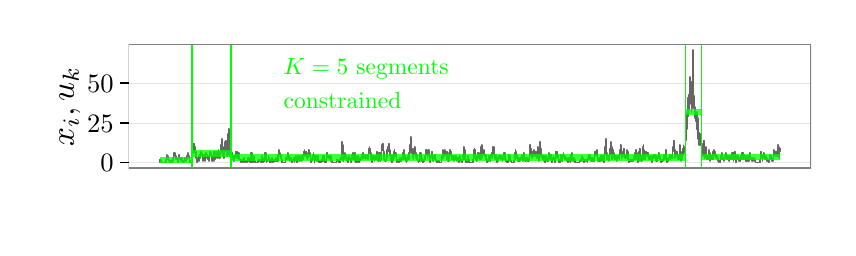
\begin{tikzpicture}[x=1pt,y=1pt]
\definecolor{fillColor}{RGB}{255,255,255}
\path[use as bounding box,fill=fillColor,fill opacity=0.00] (0,0) rectangle (289.08, 72.27);
\begin{scope}
\path[clip] (  0.00,  0.00) rectangle (289.08, 72.27);
\definecolor{drawColor}{RGB}{255,255,255}
\definecolor{fillColor}{RGB}{255,255,255}

\path[draw=drawColor,line width= 0.6pt,line join=round,line cap=round,fill=fillColor] (  0.00,  0.00) rectangle (289.08, 72.27);
\end{scope}
\begin{scope}
\path[clip] ( 36.46, 21.46) rectangle (283.08, 66.27);
\definecolor{fillColor}{RGB}{255,255,255}

\path[fill=fillColor] ( 36.46, 21.46) rectangle (283.08, 66.27);
\definecolor{drawColor}{gray}{0.90}

\path[draw=drawColor,line width= 0.2pt,line join=round] ( 36.46, 23.50) --
	(283.08, 23.50);

\path[draw=drawColor,line width= 0.2pt,line join=round] ( 36.46, 37.84) --
	(283.08, 37.84);

\path[draw=drawColor,line width= 0.2pt,line join=round] ( 36.46, 52.19) --
	(283.08, 52.19);
\definecolor{drawColor}{gray}{0.40}

\path[draw=drawColor,line width= 0.6pt,line join=round] ( 47.67, 24.07) --
	( 47.86, 24.07) --
	( 47.86, 23.50) --
	( 47.87, 23.50) --
	( 47.87, 24.07) --
	( 47.88, 24.07) --
	( 47.88, 24.65) --
	( 48.30, 24.65) --
	( 48.30, 24.07) --
	( 48.33, 24.07) --
	( 48.33, 23.50) --
	( 49.90, 23.50) --
	( 49.90, 24.07) --
	( 49.94, 24.07) --
	( 49.94, 24.65) --
	( 50.17, 24.65) --
	( 50.17, 25.22) --
	( 50.24, 25.22) --
	( 50.24, 25.80) --
	( 50.31, 25.80) --
	( 50.31, 26.37) --
	( 50.35, 26.37) --
	( 50.35, 25.80) --
	( 50.39, 25.80) --
	( 50.39, 25.22) --
	( 50.51, 25.22) --
	( 50.51, 25.80) --
	( 50.62, 25.80) --
	( 50.62, 25.22) --
	( 50.68, 25.22) --
	( 50.68, 25.80) --
	( 50.69, 25.80) --
	( 50.69, 25.22) --
	( 50.75, 25.22) --
	( 50.75, 24.65) --
	( 50.96, 24.65) --
	( 50.96, 24.07) --
	( 50.98, 24.07) --
	( 50.98, 24.65) --
	( 51.13, 24.65) --
	( 51.13, 24.07) --
	( 51.43, 24.07) --
	( 51.43, 23.50) --
	( 51.87, 23.50) --
	( 51.87, 24.07) --
	( 52.32, 24.07) --
	( 52.32, 23.50) --
	( 52.35, 23.50) --
	( 52.35, 24.07) --
	( 52.52, 24.07) --
	( 52.52, 24.65) --
	( 52.62, 24.65) --
	( 52.62, 25.22) --
	( 52.70, 25.22) --
	( 52.70, 25.80) --
	( 52.72, 25.80) --
	( 52.72, 26.37) --
	( 52.80, 26.37) --
	( 52.80, 25.80) --
	( 52.85, 25.80) --
	( 52.85, 26.37) --
	( 52.95, 26.37) --
	( 52.95, 26.94) --
	( 52.97, 26.94) --
	( 52.97, 26.37) --
	( 52.97, 26.37) --
	( 52.97, 26.94) --
	( 53.06, 26.94) --
	( 53.06, 26.37) --
	( 53.13, 26.37) --
	( 53.13, 26.94) --
	( 53.15, 26.94) --
	( 53.15, 26.37) --
	( 53.16, 26.37) --
	( 53.16, 25.80) --
	( 53.18, 25.80) --
	( 53.18, 26.37) --
	( 53.30, 26.37) --
	( 53.30, 25.80) --
	( 53.40, 25.80) --
	( 53.40, 25.22) --
	( 53.42, 25.22) --
	( 53.42, 24.65) --
	( 53.45, 24.65) --
	( 53.45, 25.22) --
	( 53.47, 25.22) --
	( 53.47, 25.80) --
	( 53.58, 25.80) --
	( 53.58, 25.22) --
	( 53.62, 25.22) --
	( 53.62, 24.65) --
	( 53.90, 24.65) --
	( 53.90, 25.22) --
	( 53.92, 25.22) --
	( 53.92, 24.65) --
	( 54.35, 24.65) --
	( 54.35, 23.50) --
	( 54.45, 23.50) --
	( 54.45, 24.07) --
	( 54.48, 24.07) --
	( 54.48, 24.65) --
	( 54.53, 24.65) --
	( 54.53, 25.22) --
	( 54.66, 25.22) --
	( 54.66, 25.80) --
	( 54.74, 25.80) --
	( 54.74, 26.37) --
	( 54.90, 26.37) --
	( 54.90, 25.80) --
	( 54.92, 25.80) --
	( 54.92, 25.22) --
	( 54.97, 25.22) --
	( 54.97, 24.65) --
	( 54.98, 24.65) --
	( 54.98, 25.22) --
	( 55.11, 25.22) --
	( 55.11, 24.65) --
	( 55.18, 24.65) --
	( 55.18, 24.07) --
	( 55.23, 24.07) --
	( 55.23, 24.65) --
	( 55.32, 24.65) --
	( 55.32, 25.22) --
	( 55.42, 25.22) --
	( 55.42, 24.65) --
	( 55.61, 24.65) --
	( 55.61, 25.22) --
	( 55.68, 25.22) --
	( 55.68, 24.65) --
	( 55.77, 24.65) --
	( 55.77, 24.07) --
	( 56.06, 24.07) --
	( 56.06, 23.50) --
	( 56.42, 23.50) --
	( 56.42, 24.07) --
	( 56.65, 24.07) --
	( 56.65, 24.65) --
	( 56.71, 24.65) --
	( 56.71, 25.22) --
	( 56.87, 25.22) --
	( 56.87, 24.65) --
	( 56.97, 24.65) --
	( 56.97, 25.22) --
	( 57.10, 25.22) --
	( 57.10, 24.65) --
	( 57.16, 24.65) --
	( 57.16, 24.07) --
	( 57.40, 24.07) --
	( 57.40, 24.65) --
	( 57.42, 24.65) --
	( 57.42, 24.07) --
	( 57.43, 24.07) --
	( 57.43, 24.65) --
	( 57.60, 24.65) --
	( 57.60, 25.80) --
	( 57.78, 25.80) --
	( 57.78, 26.37) --
	( 57.84, 26.37) --
	( 57.84, 25.80) --
	( 57.88, 25.80) --
	( 57.88, 25.22) --
	( 58.02, 25.22) --
	( 58.02, 26.37) --
	( 58.04, 26.37) --
	( 58.04, 26.94) --
	( 58.05, 26.94) --
	( 58.05, 25.80) --
	( 58.23, 25.80) --
	( 58.23, 25.22) --
	( 58.47, 25.22) --
	( 58.47, 24.07) --
	( 58.48, 24.07) --
	( 58.48, 23.50) --
	( 58.74, 23.50) --
	( 58.74, 24.07) --
	( 59.18, 24.07) --
	( 59.18, 23.50) --
	( 59.31, 23.50) --
	( 59.31, 24.07) --
	( 59.37, 24.07) --
	( 59.37, 24.65) --
	( 59.42, 24.65) --
	( 59.42, 25.80) --
	( 59.51, 25.80) --
	( 59.51, 26.94) --
	( 59.65, 26.94) --
	( 59.65, 27.52) --
	( 59.69, 27.52) --
	( 59.69, 28.09) --
	( 59.76, 28.09) --
	( 59.76, 27.52) --
	( 59.79, 27.52) --
	( 59.79, 29.24) --
	( 59.81, 29.24) --
	( 59.81, 29.81) --
	( 59.81, 29.81) --
	( 59.81, 29.24) --
	( 59.86, 29.24) --
	( 59.86, 30.39) --
	( 59.87, 30.39) --
	( 59.87, 29.24) --
	( 59.93, 29.24) --
	( 59.93, 29.81) --
	( 59.96, 29.81) --
	( 59.96, 28.66) --
	( 60.02, 28.66) --
	( 60.02, 29.24) --
	( 60.10, 29.24) --
	( 60.10, 28.66) --
	( 60.14, 28.66) --
	( 60.14, 28.09) --
	( 60.18, 28.09) --
	( 60.18, 29.81) --
	( 60.22, 29.81) --
	( 60.22, 30.39) --
	( 60.24, 30.39) --
	( 60.24, 29.81) --
	( 60.24, 29.81) --
	( 60.24, 28.66) --
	( 60.26, 28.66) --
	( 60.26, 28.09) --
	( 60.31, 28.09) --
	( 60.31, 26.94) --
	( 60.40, 26.94) --
	( 60.40, 27.52) --
	( 60.42, 27.52) --
	( 60.42, 28.09) --
	( 60.43, 28.09) --
	( 60.43, 28.66) --
	( 60.47, 28.66) --
	( 60.47, 28.09) --
	( 60.58, 28.09) --
	( 60.58, 28.66) --
	( 60.60, 28.66) --
	( 60.60, 29.24) --
	( 60.63, 29.24) --
	( 60.63, 27.52) --
	( 60.64, 27.52) --
	( 60.64, 28.09) --
	( 60.67, 28.09) --
	( 60.67, 27.52) --
	( 60.83, 27.52) --
	( 60.83, 26.94) --
	( 60.85, 26.94) --
	( 60.85, 26.37) --
	( 60.87, 26.37) --
	( 60.87, 25.22) --
	( 61.03, 25.22) --
	( 61.03, 24.07) --
	( 61.09, 24.07) --
	( 61.09, 23.50) --
	( 61.14, 23.50) --
	( 61.14, 24.07) --
	( 61.22, 24.07) --
	( 61.22, 24.65) --
	( 61.44, 24.65) --
	( 61.44, 25.22) --
	( 61.58, 25.22) --
	( 61.58, 24.65) --
	( 61.67, 24.65) --
	( 61.67, 24.07) --
	( 61.79, 24.07) --
	( 61.79, 24.65) --
	( 61.89, 24.65) --
	( 61.89, 24.07) --
	( 61.90, 24.07) --
	( 61.90, 24.65) --
	( 61.94, 24.65) --
	( 61.94, 25.22) --
	( 61.96, 25.22) --
	( 61.96, 25.80) --
	( 62.13, 25.80) --
	( 62.13, 26.37) --
	( 62.24, 26.37) --
	( 62.24, 25.80) --
	( 62.26, 25.80) --
	( 62.26, 26.37) --
	( 62.35, 26.37) --
	( 62.35, 25.80) --
	( 62.39, 25.80) --
	( 62.39, 25.22) --
	( 62.40, 25.22) --
	( 62.40, 26.37) --
	( 62.41, 26.37) --
	( 62.41, 25.80) --
	( 62.49, 25.80) --
	( 62.49, 26.37) --
	( 62.50, 26.37) --
	( 62.50, 26.94) --
	( 62.65, 26.94) --
	( 62.65, 27.52) --
	( 62.70, 27.52) --
	( 62.70, 26.94) --
	( 62.79, 26.94) --
	( 62.79, 27.52) --
	( 62.84, 27.52) --
	( 62.84, 26.37) --
	( 62.93, 26.37) --
	( 62.93, 26.94) --
	( 62.94, 26.94) --
	( 62.94, 26.37) --
	( 62.95, 26.37) --
	( 62.95, 25.80) --
	( 62.99, 25.80) --
	( 62.99, 26.94) --
	( 63.02, 26.94) --
	( 63.02, 26.37) --
	( 63.10, 26.37) --
	( 63.10, 25.80) --
	( 63.24, 25.80) --
	( 63.24, 25.22) --
	( 63.35, 25.22) --
	( 63.35, 25.80) --
	( 63.38, 25.80) --
	( 63.38, 25.22) --
	( 63.44, 25.22) --
	( 63.44, 24.07) --
	( 63.45, 24.07) --
	( 63.45, 24.65) --
	( 63.47, 24.65) --
	( 63.47, 25.22) --
	( 63.52, 25.22) --
	( 63.52, 25.80) --
	( 63.77, 25.80) --
	( 63.77, 26.37) --
	( 63.79, 26.37) --
	( 63.79, 25.80) --
	( 63.90, 25.80) --
	( 63.90, 25.22) --
	( 63.92, 25.22) --
	( 63.92, 24.65) --
	( 63.97, 24.65) --
	( 63.97, 24.07) --
	( 64.05, 24.07) --
	( 64.05, 24.65) --
	( 64.16, 24.65) --
	( 64.16, 25.22) --
	( 64.18, 25.22) --
	( 64.18, 25.80) --
	( 64.19, 25.80) --
	( 64.19, 26.37) --
	( 64.22, 26.37) --
	( 64.22, 25.80) --
	( 64.23, 25.80) --
	( 64.23, 26.37) --
	( 64.30, 26.37) --
	( 64.30, 26.94) --
	( 64.50, 26.94) --
	( 64.50, 26.37) --
	( 64.58, 26.37) --
	( 64.58, 26.94) --
	( 64.63, 26.94) --
	( 64.63, 26.37) --
	( 64.64, 26.37) --
	( 64.64, 25.80) --
	( 64.65, 25.80) --
	( 64.65, 26.37) --
	( 64.68, 26.37) --
	( 64.68, 25.80) --
	( 64.74, 25.80) --
	( 64.74, 25.22) --
	( 64.96, 25.22) --
	( 64.96, 25.80) --
	( 65.00, 25.80) --
	( 65.00, 26.37) --
	( 65.03, 26.37) --
	( 65.03, 25.80) --
	( 65.05, 25.80) --
	( 65.05, 25.22) --
	( 65.09, 25.22) --
	( 65.09, 24.65) --
	( 65.39, 24.65) --
	( 65.39, 25.22) --
	( 65.41, 25.22) --
	( 65.41, 24.65) --
	( 65.44, 24.65) --
	( 65.44, 24.07) --
	( 65.50, 24.07) --
	( 65.50, 24.65) --
	( 65.51, 24.65) --
	( 65.51, 25.22) --
	( 65.60, 25.22) --
	( 65.60, 25.80) --
	( 65.68, 25.80) --
	( 65.68, 26.37) --
	( 65.70, 26.37) --
	( 65.70, 26.94) --
	( 65.79, 26.94) --
	( 65.79, 27.52) --
	( 65.84, 27.52) --
	( 65.84, 26.94) --
	( 65.93, 26.94) --
	( 65.93, 27.52) --
	( 65.94, 27.52) --
	( 65.94, 26.94) --
	( 65.95, 26.94) --
	( 65.95, 26.37) --
	( 66.01, 26.37) --
	( 66.01, 25.80) --
	( 66.05, 25.80) --
	( 66.05, 26.37) --
	( 66.12, 26.37) --
	( 66.12, 26.94) --
	( 66.13, 26.94) --
	( 66.13, 26.37) --
	( 66.13, 26.37) --
	( 66.13, 26.94) --
	( 66.15, 26.94) --
	( 66.15, 26.37) --
	( 66.18, 26.37) --
	( 66.18, 26.94) --
	( 66.24, 26.94) --
	( 66.24, 26.37) --
	( 66.30, 26.37) --
	( 66.30, 26.94) --
	( 66.38, 26.94) --
	( 66.38, 26.37) --
	( 66.50, 26.37) --
	( 66.50, 25.80) --
	( 66.57, 25.80) --
	( 66.57, 25.22) --
	( 66.58, 25.22) --
	( 66.58, 24.65) --
	( 66.63, 24.65) --
	( 66.63, 24.07) --
	( 66.65, 24.07) --
	( 66.65, 24.65) --
	( 66.67, 24.65) --
	( 66.67, 24.07) --
	( 66.81, 24.07) --
	( 66.81, 24.65) --
	( 67.05, 24.65) --
	( 67.05, 25.22) --
	( 67.10, 25.22) --
	( 67.10, 24.65) --
	( 67.26, 24.65) --
	( 67.26, 24.07) --
	( 67.28, 24.07) --
	( 67.28, 25.22) --
	( 67.30, 25.22) --
	( 67.30, 25.80) --
	( 67.32, 25.80) --
	( 67.32, 26.37) --
	( 67.34, 26.37) --
	( 67.34, 26.94) --
	( 67.38, 26.94) --
	( 67.38, 27.52) --
	( 67.50, 27.52) --
	( 67.50, 26.94) --
	( 67.57, 26.94) --
	( 67.57, 27.52) --
	( 67.73, 27.52) --
	( 67.73, 26.37) --
	( 67.75, 26.37) --
	( 67.75, 25.80) --
	( 67.76, 25.80) --
	( 67.76, 25.22) --
	( 67.82, 25.22) --
	( 67.82, 24.65) --
	( 67.91, 24.65) --
	( 67.91, 25.22) --
	( 67.93, 25.22) --
	( 67.93, 26.37) --
	( 68.05, 26.37) --
	( 68.05, 26.94) --
	( 68.09, 26.94) --
	( 68.09, 27.52) --
	( 68.24, 27.52) --
	( 68.24, 26.94) --
	( 68.35, 26.94) --
	( 68.35, 26.37) --
	( 68.38, 26.37) --
	( 68.38, 25.22) --
	( 68.40, 25.22) --
	( 68.40, 25.80) --
	( 68.47, 25.80) --
	( 68.47, 25.22) --
	( 68.49, 25.22) --
	( 68.49, 25.80) --
	( 68.50, 25.80) --
	( 68.50, 25.22) --
	( 68.53, 25.22) --
	( 68.53, 25.80) --
	( 68.54, 25.80) --
	( 68.54, 25.22) --
	( 68.60, 25.22) --
	( 68.60, 25.80) --
	( 68.67, 25.80) --
	( 68.67, 26.37) --
	( 68.70, 26.37) --
	( 68.70, 26.94) --
	( 68.78, 26.94) --
	( 68.78, 27.52) --
	( 68.85, 27.52) --
	( 68.85, 26.94) --
	( 68.85, 26.94) --
	( 68.85, 27.52) --
	( 68.94, 27.52) --
	( 68.94, 26.94) --
	( 68.97, 26.94) --
	( 68.97, 27.52) --
	( 68.97, 27.52) --
	( 68.97, 28.09) --
	( 68.98, 28.09) --
	( 68.98, 27.52) --
	( 69.04, 27.52) --
	( 69.04, 26.94) --
	( 69.12, 26.94) --
	( 69.12, 26.37) --
	( 69.15, 26.37) --
	( 69.15, 25.80) --
	( 69.22, 25.80) --
	( 69.22, 25.22) --
	( 69.23, 25.22) --
	( 69.23, 25.80) --
	( 69.26, 25.80) --
	( 69.26, 26.94) --
	( 69.30, 26.94) --
	( 69.30, 26.37) --
	( 69.42, 26.37) --
	( 69.42, 25.80) --
	( 69.42, 25.80) --
	( 69.42, 25.22) --
	( 69.44, 25.22) --
	( 69.44, 25.80) --
	( 69.49, 25.80) --
	( 69.49, 26.37) --
	( 69.56, 26.37) --
	( 69.56, 26.94) --
	( 69.66, 26.94) --
	( 69.66, 27.52) --
	( 69.68, 27.52) --
	( 69.68, 26.94) --
	( 69.69, 26.94) --
	( 69.69, 27.52) --
	( 69.70, 27.52) --
	( 69.70, 28.09) --
	( 69.71, 28.09) --
	( 69.71, 27.52) --
	( 69.71, 27.52) --
	( 69.71, 26.94) --
	( 69.74, 26.94) --
	( 69.74, 27.52) --
	( 69.88, 27.52) --
	( 69.88, 28.09) --
	( 69.89, 28.09) --
	( 69.89, 27.52) --
	( 69.93, 27.52) --
	( 69.93, 28.09) --
	( 69.94, 28.09) --
	( 69.94, 27.52) --
	( 69.96, 27.52) --
	( 69.96, 29.24) --
	( 69.96, 29.24) --
	( 69.96, 29.81) --
	( 69.99, 29.81) --
	( 69.99, 29.24) --
	( 70.01, 29.24) --
	( 70.01, 29.81) --
	( 70.05, 29.81) --
	( 70.05, 30.39) --
	( 70.09, 30.39) --
	( 70.09, 30.96) --
	( 70.11, 30.96) --
	( 70.11, 30.39) --
	( 70.14, 30.39) --
	( 70.14, 29.81) --
	( 70.15, 29.81) --
	( 70.15, 29.24) --
	( 70.16, 29.24) --
	( 70.16, 29.81) --
	( 70.18, 29.81) --
	( 70.18, 30.39) --
	( 70.19, 30.39) --
	( 70.19, 29.81) --
	( 70.20, 29.81) --
	( 70.20, 30.96) --
	( 70.26, 30.96) --
	( 70.26, 31.53) --
	( 70.32, 31.53) --
	( 70.32, 32.11) --
	( 70.33, 32.11) --
	( 70.33, 31.53) --
	( 70.38, 31.53) --
	( 70.38, 30.96) --
	( 70.41, 30.96) --
	( 70.41, 29.24) --
	( 70.41, 29.24) --
	( 70.41, 28.09) --
	( 70.43, 28.09) --
	( 70.43, 28.66) --
	( 70.48, 28.66) --
	( 70.48, 29.24) --
	( 70.50, 29.24) --
	( 70.50, 28.66) --
	( 70.54, 28.66) --
	( 70.54, 28.09) --
	( 70.56, 28.09) --
	( 70.56, 27.52) --
	( 70.63, 27.52) --
	( 70.63, 26.94) --
	( 70.65, 26.94) --
	( 70.65, 25.80) --
	( 70.69, 25.80) --
	( 70.69, 26.37) --
	( 70.70, 26.37) --
	( 70.70, 25.22) --
	( 70.79, 25.22) --
	( 70.79, 25.80) --
	( 70.87, 25.80) --
	( 70.87, 26.37) --
	( 70.87, 26.37) --
	( 70.87, 25.80) --
	( 70.93, 25.80) --
	( 70.93, 25.22) --
	( 71.00, 25.22) --
	( 71.00, 26.37) --
	( 71.04, 26.37) --
	( 71.04, 26.94) --
	( 71.08, 26.94) --
	( 71.08, 27.52) --
	( 71.08, 27.52) --
	( 71.08, 26.94) --
	( 71.15, 26.94) --
	( 71.15, 27.52) --
	( 71.17, 27.52) --
	( 71.17, 28.09) --
	( 71.24, 28.09) --
	( 71.24, 27.52) --
	( 71.27, 27.52) --
	( 71.27, 28.09) --
	( 71.27, 28.09) --
	( 71.27, 28.66) --
	( 71.31, 28.66) --
	( 71.31, 29.24) --
	( 71.33, 29.24) --
	( 71.33, 28.66) --
	( 71.35, 28.66) --
	( 71.35, 29.24) --
	( 71.39, 29.24) --
	( 71.39, 29.81) --
	( 71.40, 29.81) --
	( 71.40, 30.39) --
	( 71.41, 30.39) --
	( 71.41, 30.96) --
	( 71.46, 30.96) --
	( 71.46, 31.53) --
	( 71.48, 31.53) --
	( 71.48, 30.96) --
	( 71.51, 30.96) --
	( 71.51, 31.53) --
	( 71.52, 31.53) --
	( 71.52, 30.96) --
	( 71.53, 30.96) --
	( 71.53, 30.39) --
	( 71.56, 30.39) --
	( 71.56, 30.96) --
	( 71.57, 30.96) --
	( 71.57, 31.53) --
	( 71.60, 31.53) --
	( 71.60, 30.96) --
	( 71.67, 30.96) --
	( 71.67, 31.53) --
	( 71.72, 31.53) --
	( 71.72, 30.96) --
	( 71.75, 30.96) --
	( 71.75, 30.39) --
	( 71.76, 30.39) --
	( 71.76, 30.96) --
	( 71.77, 30.96) --
	( 71.77, 30.39) --
	( 71.80, 30.39) --
	( 71.80, 30.96) --
	( 71.83, 30.96) --
	( 71.83, 30.39) --
	( 71.85, 30.39) --
	( 71.85, 29.81) --
	( 71.86, 29.81) --
	( 71.86, 29.24) --
	( 71.89, 29.24) --
	( 71.89, 28.66) --
	( 71.91, 28.66) --
	( 71.91, 28.09) --
	( 71.95, 28.09) --
	( 71.95, 27.52) --
	( 72.00, 27.52) --
	( 72.00, 26.94) --
	( 72.00, 26.94) --
	( 72.00, 27.52) --
	( 72.01, 27.52) --
	( 72.01, 26.94) --
	( 72.02, 26.94) --
	( 72.02, 26.37) --
	( 72.07, 26.37) --
	( 72.07, 25.80) --
	( 72.08, 25.80) --
	( 72.08, 26.37) --
	( 72.11, 26.37) --
	( 72.11, 26.94) --
	( 72.12, 26.94) --
	( 72.12, 26.37) --
	( 72.19, 26.37) --
	( 72.19, 26.94) --
	( 72.21, 26.94) --
	( 72.21, 26.37) --
	( 72.25, 26.37) --
	( 72.25, 25.80) --
	( 72.26, 25.80) --
	( 72.26, 26.37) --
	( 72.27, 26.37) --
	( 72.27, 27.52) --
	( 72.28, 27.52) --
	( 72.28, 28.09) --
	( 72.34, 28.09) --
	( 72.34, 28.66) --
	( 72.37, 28.66) --
	( 72.37, 29.24) --
	( 72.38, 29.24) --
	( 72.38, 29.81) --
	( 72.39, 29.81) --
	( 72.39, 30.39) --
	( 72.43, 30.39) --
	( 72.43, 30.96) --
	( 72.44, 30.96) --
	( 72.44, 31.53) --
	( 72.45, 31.53) --
	( 72.45, 30.96) --
	( 72.46, 30.96) --
	( 72.46, 31.53) --
	( 72.47, 31.53) --
	( 72.47, 33.25) --
	( 72.49, 33.25) --
	( 72.49, 33.83) --
	( 72.51, 33.83) --
	( 72.51, 33.25) --
	( 72.52, 33.25) --
	( 72.52, 33.83) --
	( 72.53, 33.83) --
	( 72.53, 34.40) --
	( 72.55, 34.40) --
	( 72.55, 34.98) --
	( 72.56, 34.98) --
	( 72.56, 35.55) --
	( 72.56, 35.55) --
	( 72.56, 34.98) --
	( 72.61, 34.98) --
	( 72.61, 35.55) --
	( 72.64, 35.55) --
	( 72.64, 34.98) --
	( 72.71, 34.98) --
	( 72.71, 34.40) --
	( 72.72, 34.40) --
	( 72.72, 33.83) --
	( 72.73, 33.83) --
	( 72.73, 33.25) --
	( 72.78, 33.25) --
	( 72.78, 32.68) --
	( 72.82, 32.68) --
	( 72.82, 32.11) --
	( 72.83, 32.11) --
	( 72.83, 31.53) --
	( 72.83, 31.53) --
	( 72.83, 30.96) --
	( 72.87, 30.96) --
	( 72.87, 30.39) --
	( 72.89, 30.39) --
	( 72.89, 29.81) --
	( 72.91, 29.81) --
	( 72.91, 29.24) --
	( 72.92, 29.24) --
	( 72.92, 27.52) --
	( 72.93, 27.52) --
	( 72.93, 28.09) --
	( 72.94, 28.09) --
	( 72.94, 26.94) --
	( 72.97, 26.94) --
	( 72.97, 26.37) --
	( 72.98, 26.37) --
	( 72.98, 25.80) --
	( 72.99, 25.80) --
	( 72.99, 26.37) --
	( 72.99, 26.37) --
	( 72.99, 26.94) --
	( 73.01, 26.94) --
	( 73.01, 26.37) --
	( 73.06, 26.37) --
	( 73.06, 25.80) --
	( 73.18, 25.80) --
	( 73.18, 26.94) --
	( 73.38, 26.94) --
	( 73.38, 26.37) --
	( 73.44, 26.37) --
	( 73.44, 24.65) --
	( 73.60, 24.65) --
	( 73.60, 25.80) --
	( 73.63, 25.80) --
	( 73.63, 24.65) --
	( 73.71, 24.65) --
	( 73.71, 25.22) --
	( 73.84, 25.22) --
	( 73.84, 25.80) --
	( 73.98, 25.80) --
	( 73.98, 26.37) --
	( 73.99, 26.37) --
	( 73.99, 26.94) --
	( 74.05, 26.94) --
	( 74.05, 25.80) --
	( 74.15, 25.80) --
	( 74.15, 25.22) --
	( 74.29, 25.22) --
	( 74.29, 24.65) --
	( 74.30, 24.65) --
	( 74.30, 25.22) --
	( 74.43, 25.22) --
	( 74.43, 24.65) --
	( 74.43, 24.65) --
	( 74.43, 24.07) --
	( 74.46, 24.07) --
	( 74.46, 24.65) --
	( 74.46, 24.65) --
	( 74.46, 25.22) --
	( 74.73, 25.22) --
	( 74.73, 25.80) --
	( 74.74, 25.80) --
	( 74.74, 25.22) --
	( 74.88, 25.22) --
	( 74.88, 25.80) --
	( 74.91, 25.80) --
	( 74.91, 25.22) --
	( 74.98, 25.22) --
	( 74.98, 25.80) --
	( 75.11, 25.80) --
	( 75.11, 26.37) --
	( 75.18, 26.37) --
	( 75.18, 25.80) --
	( 75.22, 25.80) --
	( 75.22, 26.37) --
	( 75.28, 26.37) --
	( 75.28, 27.52) --
	( 75.33, 27.52) --
	( 75.33, 26.94) --
	( 75.35, 26.94) --
	( 75.35, 26.37) --
	( 75.43, 26.37) --
	( 75.43, 25.80) --
	( 75.48, 25.80) --
	( 75.48, 26.37) --
	( 75.49, 26.37) --
	( 75.49, 26.94) --
	( 75.56, 26.94) --
	( 75.56, 26.37) --
	( 75.60, 26.37) --
	( 75.60, 26.94) --
	( 75.64, 26.94) --
	( 75.64, 27.52) --
	( 75.65, 27.52) --
	( 75.65, 26.94) --
	( 75.66, 26.94) --
	( 75.66, 26.37) --
	( 75.69, 26.37) --
	( 75.69, 25.80) --
	( 75.72, 25.80) --
	( 75.72, 25.22) --
	( 75.80, 25.22) --
	( 75.80, 25.80) --
	( 75.82, 25.80) --
	( 75.82, 26.37) --
	( 75.86, 26.37) --
	( 75.86, 25.80) --
	( 75.94, 25.80) --
	( 75.94, 25.22) --
	( 75.96, 25.22) --
	( 75.96, 25.80) --
	( 75.96, 25.80) --
	( 75.96, 26.37) --
	( 76.06, 26.37) --
	( 76.06, 26.94) --
	( 76.09, 26.94) --
	( 76.09, 26.37) --
	( 76.09, 26.37) --
	( 76.09, 26.94) --
	( 76.25, 26.94) --
	( 76.25, 26.37) --
	( 76.27, 26.37) --
	( 76.27, 25.80) --
	( 76.40, 25.80) --
	( 76.40, 24.65) --
	( 76.48, 24.65) --
	( 76.48, 25.22) --
	( 76.51, 25.22) --
	( 76.51, 24.65) --
	( 76.51, 24.65) --
	( 76.51, 25.22) --
	( 76.54, 25.22) --
	( 76.54, 24.65) --
	( 76.93, 24.65) --
	( 76.93, 24.07) --
	( 76.96, 24.07) --
	( 76.96, 23.50) --
	( 77.15, 23.50) --
	( 77.15, 24.07) --
	( 77.26, 24.07) --
	( 77.26, 24.65) --
	( 77.55, 24.65) --
	( 77.55, 24.07) --
	( 77.71, 24.07) --
	( 77.71, 23.50) --
	( 77.90, 23.50) --
	( 77.90, 24.07) --
	( 77.95, 24.07) --
	( 77.95, 24.65) --
	( 77.96, 24.65) --
	( 77.96, 25.22) --
	( 78.34, 25.22) --
	( 78.34, 24.65) --
	( 78.40, 24.65) --
	( 78.40, 24.07) --
	( 78.41, 24.07) --
	( 78.41, 23.50) --
	( 78.64, 23.50) --
	( 78.64, 24.07) --
	( 79.09, 24.07) --
	( 79.09, 23.50) --
	( 79.30, 23.50) --
	( 79.30, 24.07) --
	( 79.43, 24.07) --
	( 79.43, 24.65) --
	( 79.60, 24.65) --
	( 79.60, 25.22) --
	( 79.64, 25.22) --
	( 79.64, 24.65) --
	( 79.75, 24.65) --
	( 79.75, 24.07) --
	( 79.92, 24.07) --
	( 79.92, 24.65) --
	( 79.97, 24.65) --
	( 79.97, 25.22) --
	( 80.05, 25.22) --
	( 80.05, 24.65) --
	( 80.36, 24.65) --
	( 80.36, 24.07) --
	( 80.42, 24.07) --
	( 80.42, 23.50) --
	( 80.60, 23.50) --
	( 80.60, 25.22) --
	( 80.63, 25.22) --
	( 80.63, 26.94) --
	( 81.04, 26.94) --
	( 81.04, 25.22) --
	( 81.07, 25.22) --
	( 81.07, 24.65) --
	( 81.07, 24.65) --
	( 81.07, 23.50) --
	( 81.32, 23.50) --
	( 81.32, 24.07) --
	( 81.35, 24.07) --
	( 81.35, 24.65) --
	( 81.53, 24.65) --
	( 81.53, 25.22) --
	( 81.68, 25.22) --
	( 81.68, 25.80) --
	( 81.73, 25.80) --
	( 81.73, 25.22) --
	( 81.80, 25.22) --
	( 81.80, 24.65) --
	( 81.98, 24.65) --
	( 81.98, 24.07) --
	( 82.12, 24.07) --
	( 82.12, 23.50) --
	( 83.16, 23.50) --
	( 83.16, 24.07) --
	( 83.40, 24.07) --
	( 83.40, 24.65) --
	( 83.61, 24.65) --
	( 83.61, 24.07) --
	( 83.64, 24.07) --
	( 83.64, 24.65) --
	( 83.85, 24.65) --
	( 83.85, 24.07) --
	( 83.90, 24.07) --
	( 83.90, 24.65) --
	( 84.08, 24.65) --
	( 84.08, 24.07) --
	( 84.34, 24.07) --
	( 84.34, 23.50) --
	( 84.38, 23.50) --
	( 84.38, 24.07) --
	( 84.61, 24.07) --
	( 84.61, 24.65) --
	( 84.63, 24.65) --
	( 84.63, 25.22) --
	( 84.65, 25.22) --
	( 84.65, 25.80) --
	( 84.83, 25.80) --
	( 84.83, 25.22) --
	( 85.06, 25.22) --
	( 85.06, 24.65) --
	( 85.08, 24.65) --
	( 85.08, 24.07) --
	( 85.10, 24.07) --
	( 85.10, 23.50) --
	( 85.20, 23.50) --
	( 85.20, 24.07) --
	( 85.58, 24.07) --
	( 85.58, 24.65) --
	( 85.65, 24.65) --
	( 85.65, 24.07) --
	( 85.73, 24.07) --
	( 85.73, 24.65) --
	( 85.81, 24.65) --
	( 85.81, 25.22) --
	( 85.84, 25.22) --
	( 85.84, 26.37) --
	( 85.85, 26.37) --
	( 85.85, 26.94) --
	( 86.02, 26.94) --
	( 86.02, 26.37) --
	( 86.17, 26.37) --
	( 86.17, 25.80) --
	( 86.25, 25.80) --
	( 86.25, 25.22) --
	( 86.29, 25.22) --
	( 86.29, 24.07) --
	( 86.30, 24.07) --
	( 86.30, 23.50) --
	( 86.33, 23.50) --
	( 86.33, 24.07) --
	( 86.56, 24.07) --
	( 86.56, 24.65) --
	( 86.78, 24.65) --
	( 86.78, 24.07) --
	( 86.91, 24.07) --
	( 86.91, 24.65) --
	( 86.97, 24.65) --
	( 86.97, 25.80) --
	( 87.01, 25.80) --
	( 87.01, 25.22) --
	( 87.36, 25.22) --
	( 87.36, 24.65) --
	( 87.41, 24.65) --
	( 87.41, 23.50) --
	( 87.47, 23.50) --
	( 87.47, 24.07) --
	( 87.71, 24.07) --
	( 87.71, 24.65) --
	( 87.92, 24.65) --
	( 87.92, 23.50) --
	( 87.98, 23.50) --
	( 87.98, 24.07) --
	( 88.13, 24.07) --
	( 88.13, 24.65) --
	( 88.38, 24.65) --
	( 88.38, 25.22) --
	( 88.41, 25.22) --
	( 88.41, 24.65) --
	( 88.57, 24.65) --
	( 88.57, 23.50) --
	( 88.82, 23.50) --
	( 88.82, 24.07) --
	( 89.25, 24.07) --
	( 89.25, 24.65) --
	( 89.27, 24.65) --
	( 89.27, 24.07) --
	( 89.35, 24.07) --
	( 89.35, 24.65) --
	( 89.51, 24.65) --
	( 89.51, 25.22) --
	( 89.69, 25.22) --
	( 89.69, 24.65) --
	( 89.80, 24.65) --
	( 89.80, 24.07) --
	( 89.81, 24.07) --
	( 89.81, 24.65) --
	( 89.94, 24.65) --
	( 89.94, 24.07) --
	( 90.07, 24.07) --
	( 90.07, 24.65) --
	( 90.26, 24.65) --
	( 90.26, 24.07) --
	( 90.41, 24.07) --
	( 90.41, 24.65) --
	( 90.43, 24.65) --
	( 90.43, 25.22) --
	( 90.48, 25.22) --
	( 90.48, 26.37) --
	( 90.52, 26.37) --
	( 90.52, 25.80) --
	( 90.55, 25.80) --
	( 90.55, 26.37) --
	( 90.59, 26.37) --
	( 90.59, 26.94) --
	( 90.69, 26.94) --
	( 90.69, 27.52) --
	( 90.80, 27.52) --
	( 90.80, 28.09) --
	( 90.86, 28.09) --
	( 90.86, 27.52) --
	( 90.87, 27.52) --
	( 90.87, 28.09) --
	( 90.88, 28.09) --
	( 90.88, 27.52) --
	( 90.93, 27.52) --
	( 90.93, 26.37) --
	( 90.99, 26.37) --
	( 90.99, 26.94) --
	( 91.00, 26.94) --
	( 91.00, 26.37) --
	( 91.01, 26.37) --
	( 91.01, 26.94) --
	( 91.03, 26.94) --
	( 91.03, 26.37) --
	( 91.11, 26.37) --
	( 91.11, 26.94) --
	( 91.14, 26.94) --
	( 91.14, 26.37) --
	( 91.25, 26.37) --
	( 91.25, 25.80) --
	( 91.28, 25.80) --
	( 91.28, 26.37) --
	( 91.32, 26.37) --
	( 91.32, 25.80) --
	( 91.38, 25.80) --
	( 91.38, 26.37) --
	( 91.44, 26.37) --
	( 91.44, 25.80) --
	( 91.45, 25.80) --
	( 91.45, 25.22) --
	( 91.52, 25.22) --
	( 91.52, 25.80) --
	( 91.56, 25.80) --
	( 91.56, 25.22) --
	( 91.73, 25.22) --
	( 91.73, 24.65) --
	( 91.83, 24.65) --
	( 91.83, 24.07) --
	( 91.97, 24.07) --
	( 91.97, 23.50) --
	( 93.19, 23.50) --
	( 93.19, 24.07) --
	( 93.21, 24.07) --
	( 93.21, 24.65) --
	( 93.35, 24.65) --
	( 93.35, 25.22) --
	( 93.63, 25.22) --
	( 93.63, 24.65) --
	( 93.63, 24.65) --
	( 93.63, 25.22) --
	( 93.66, 25.22) --
	( 93.66, 25.80) --
	( 93.66, 25.80) --
	( 93.66, 25.22) --
	( 93.80, 25.22) --
	( 93.80, 24.65) --
	( 93.89, 24.65) --
	( 93.89, 25.22) --
	( 93.96, 25.22) --
	( 93.96, 25.80) --
	( 94.06, 25.80) --
	( 94.06, 26.94) --
	( 94.08, 26.94) --
	( 94.08, 26.37) --
	( 94.10, 26.37) --
	( 94.10, 25.80) --
	( 94.33, 25.80) --
	( 94.33, 25.22) --
	( 94.37, 25.22) --
	( 94.37, 25.80) --
	( 94.41, 25.80) --
	( 94.41, 25.22) --
	( 94.43, 25.22) --
	( 94.43, 25.80) --
	( 94.51, 25.80) --
	( 94.51, 24.65) --
	( 94.78, 24.65) --
	( 94.78, 25.22) --
	( 94.82, 25.22) --
	( 94.82, 24.65) --
	( 94.88, 24.65) --
	( 94.88, 24.07) --
	( 94.90, 24.07) --
	( 94.90, 24.65) --
	( 94.98, 24.65) --
	( 94.98, 25.22) --
	( 95.23, 25.22) --
	( 95.23, 24.65) --
	( 95.35, 24.65) --
	( 95.35, 24.07) --
	( 95.43, 24.07) --
	( 95.43, 23.50) --
	( 95.67, 23.50) --
	( 95.67, 24.07) --
	( 95.68, 24.07) --
	( 95.68, 24.65) --
	( 96.00, 24.65) --
	( 96.00, 25.22) --
	( 96.12, 25.22) --
	( 96.12, 24.07) --
	( 96.45, 24.07) --
	( 96.45, 23.50) --
	( 96.46, 23.50) --
	( 96.46, 24.07) --
	( 96.64, 24.07) --
	( 96.64, 24.65) --
	( 96.71, 24.65) --
	( 96.71, 25.22) --
	( 96.74, 25.22) --
	( 96.74, 25.80) --
	( 96.91, 25.80) --
	( 96.91, 25.22) --
	( 97.09, 25.22) --
	( 97.09, 24.65) --
	( 97.16, 24.65) --
	( 97.16, 24.07) --
	( 97.19, 24.07) --
	( 97.19, 23.50) --
	( 97.24, 23.50) --
	( 97.24, 24.07) --
	( 97.61, 24.07) --
	( 97.61, 24.65) --
	( 97.68, 24.65) --
	( 97.68, 25.22) --
	( 97.69, 25.22) --
	( 97.69, 24.65) --
	( 97.69, 24.65) --
	( 97.69, 25.22) --
	( 97.80, 25.22) --
	( 97.80, 25.80) --
	( 98.06, 25.80) --
	( 98.06, 25.22) --
	( 98.08, 25.22) --
	( 98.08, 25.80) --
	( 98.13, 25.80) --
	( 98.13, 25.22) --
	( 98.14, 25.22) --
	( 98.14, 24.65) --
	( 98.24, 24.65) --
	( 98.24, 24.07) --
	( 98.37, 24.07) --
	( 98.37, 24.65) --
	( 98.45, 24.65) --
	( 98.45, 25.22) --
	( 98.53, 25.22) --
	( 98.53, 24.65) --
	( 98.58, 24.65) --
	( 98.58, 25.22) --
	( 98.67, 25.22) --
	( 98.67, 25.80) --
	( 98.81, 25.80) --
	( 98.81, 25.22) --
	( 98.83, 25.22) --
	( 98.83, 25.80) --
	( 98.90, 25.80) --
	( 98.90, 25.22) --
	( 99.03, 25.22) --
	( 99.03, 24.65) --
	( 99.12, 24.65) --
	( 99.12, 24.07) --
	( 99.14, 24.07) --
	( 99.14, 24.65) --
	( 99.17, 24.65) --
	( 99.17, 25.22) --
	( 99.28, 25.22) --
	( 99.28, 24.65) --
	( 99.33, 24.65) --
	( 99.33, 25.22) --
	( 99.41, 25.22) --
	( 99.41, 24.65) --
	( 99.43, 24.65) --
	( 99.43, 25.22) --
	( 99.54, 25.22) --
	( 99.54, 25.80) --
	( 99.58, 25.80) --
	( 99.58, 26.37) --
	( 99.64, 26.37) --
	( 99.64, 26.94) --
	( 99.72, 26.94) --
	( 99.72, 27.52) --
	( 99.78, 27.52) --
	( 99.78, 26.94) --
	( 99.87, 26.94) --
	( 99.87, 26.37) --
	( 99.92, 26.37) --
	( 99.92, 26.94) --
	( 99.92, 26.94) --
	( 99.92, 27.52) --
	( 99.98, 27.52) --
	( 99.98, 28.09) --
	( 99.99, 28.09) --
	( 99.99, 27.52) --
	(100.02, 27.52) --
	(100.02, 26.94) --
	(100.05, 26.94) --
	(100.05, 27.52) --
	(100.07, 27.52) --
	(100.07, 26.37) --
	(100.17, 26.37) --
	(100.17, 25.80) --
	(100.18, 25.80) --
	(100.18, 26.37) --
	(100.33, 26.37) --
	(100.33, 26.94) --
	(100.36, 26.94) --
	(100.36, 26.37) --
	(100.37, 26.37) --
	(100.37, 25.80) --
	(100.37, 25.80) --
	(100.37, 26.37) --
	(100.40, 26.37) --
	(100.40, 26.94) --
	(100.42, 26.94) --
	(100.42, 27.52) --
	(100.43, 27.52) --
	(100.43, 26.94) --
	(100.46, 26.94) --
	(100.46, 27.52) --
	(100.50, 27.52) --
	(100.50, 26.94) --
	(100.60, 26.94) --
	(100.60, 27.52) --
	(100.62, 27.52) --
	(100.62, 26.94) --
	(100.71, 26.94) --
	(100.71, 27.52) --
	(100.78, 27.52) --
	(100.78, 26.94) --
	(100.82, 26.94) --
	(100.82, 26.37) --
	(100.85, 26.37) --
	(100.85, 25.80) --
	(100.86, 25.80) --
	(100.86, 26.37) --
	(100.91, 26.37) --
	(100.91, 25.80) --
	(101.05, 25.80) --
	(101.05, 25.22) --
	(101.06, 25.22) --
	(101.06, 24.65) --
	(101.09, 24.65) --
	(101.09, 25.22) --
	(101.10, 25.22) --
	(101.10, 25.80) --
	(101.31, 25.80) --
	(101.31, 25.22) --
	(101.38, 25.22) --
	(101.38, 25.80) --
	(101.44, 25.80) --
	(101.44, 26.37) --
	(101.46, 26.37) --
	(101.46, 26.94) --
	(101.52, 26.94) --
	(101.52, 28.09) --
	(101.54, 28.09) --
	(101.54, 27.52) --
	(101.54, 27.52) --
	(101.54, 26.94) --
	(101.58, 26.94) --
	(101.58, 27.52) --
	(101.60, 27.52) --
	(101.60, 26.94) --
	(101.69, 26.94) --
	(101.69, 27.52) --
	(101.83, 27.52) --
	(101.83, 26.94) --
	(101.88, 26.94) --
	(101.88, 26.37) --
	(101.91, 26.37) --
	(101.91, 25.80) --
	(101.93, 25.80) --
	(101.93, 26.94) --
	(101.97, 26.94) --
	(101.97, 26.37) --
	(101.97, 26.37) --
	(101.97, 25.80) --
	(101.97, 25.80) --
	(101.97, 26.37) --
	(102.02, 26.37) --
	(102.02, 25.80) --
	(102.14, 25.80) --
	(102.14, 25.22) --
	(102.38, 25.22) --
	(102.38, 24.07) --
	(102.42, 24.07) --
	(102.42, 23.50) --
	(102.49, 23.50) --
	(102.49, 24.07) --
	(102.71, 24.07) --
	(102.71, 24.65) --
	(102.87, 24.65) --
	(102.87, 25.22) --
	(102.93, 25.22) --
	(102.93, 24.65) --
	(103.11, 24.65) --
	(103.11, 25.80) --
	(103.16, 25.80) --
	(103.16, 25.22) --
	(103.17, 25.22) --
	(103.17, 26.37) --
	(103.24, 26.37) --
	(103.24, 26.94) --
	(103.32, 26.94) --
	(103.32, 26.37) --
	(103.34, 26.37) --
	(103.34, 25.80) --
	(103.38, 25.80) --
	(103.38, 26.37) --
	(103.56, 26.37) --
	(103.56, 25.80) --
	(103.61, 25.80) --
	(103.61, 25.22) --
	(103.62, 25.22) --
	(103.62, 24.65) --
	(103.69, 24.65) --
	(103.69, 23.50) --
	(103.69, 23.50) --
	(103.69, 24.07) --
	(103.86, 24.07) --
	(103.86, 24.65) --
	(103.99, 24.65) --
	(103.99, 25.22) --
	(104.03, 25.22) --
	(104.03, 25.80) --
	(104.14, 25.80) --
	(104.14, 25.22) --
	(104.31, 25.22) --
	(104.31, 24.65) --
	(104.44, 24.65) --
	(104.44, 24.07) --
	(104.47, 24.07) --
	(104.47, 24.65) --
	(104.50, 24.65) --
	(104.50, 25.22) --
	(104.72, 25.22) --
	(104.72, 25.80) --
	(104.92, 25.80) --
	(104.92, 25.22) --
	(104.92, 25.22) --
	(104.92, 24.65) --
	(104.95, 24.65) --
	(104.95, 24.07) --
	(105.17, 24.07) --
	(105.17, 23.50) --
	(105.18, 23.50) --
	(105.18, 24.07) --
	(105.63, 24.07) --
	(105.63, 23.50) --
	(105.97, 23.50) --
	(105.97, 24.07) --
	(106.16, 24.07) --
	(106.16, 24.65) --
	(106.29, 24.65) --
	(106.29, 24.07) --
	(106.56, 24.07) --
	(106.56, 24.65) --
	(106.61, 24.65) --
	(106.61, 24.07) --
	(106.61, 24.07) --
	(106.61, 24.65) --
	(106.65, 24.65) --
	(106.65, 25.22) --
	(106.78, 25.22) --
	(106.78, 25.80) --
	(107.01, 25.80) --
	(107.01, 25.22) --
	(107.06, 25.22) --
	(107.06, 24.65) --
	(107.09, 24.65) --
	(107.09, 24.07) --
	(107.23, 24.07) --
	(107.23, 23.50) --
	(107.68, 23.50) --
	(107.68, 24.07) --
	(107.84, 24.07) --
	(107.84, 24.65) --
	(107.93, 24.65) --
	(107.93, 25.22) --
	(107.99, 25.22) --
	(107.99, 25.80) --
	(108.05, 25.80) --
	(108.05, 26.37) --
	(108.13, 26.37) --
	(108.13, 25.80) --
	(108.25, 25.80) --
	(108.25, 26.37) --
	(108.27, 26.37) --
	(108.27, 26.94) --
	(108.29, 26.94) --
	(108.29, 26.37) --
	(108.38, 26.37) --
	(108.38, 25.80) --
	(108.44, 25.80) --
	(108.44, 25.22) --
	(108.48, 25.22) --
	(108.48, 25.80) --
	(108.50, 25.80) --
	(108.50, 25.22) --
	(108.61, 25.22) --
	(108.61, 25.80) --
	(108.70, 25.80) --
	(108.70, 25.22) --
	(108.84, 25.22) --
	(108.84, 25.80) --
	(108.93, 25.80) --
	(108.93, 25.22) --
	(108.93, 25.22) --
	(108.93, 25.80) --
	(109.06, 25.80) --
	(109.06, 25.22) --
	(109.16, 25.22) --
	(109.16, 24.65) --
	(109.17, 24.65) --
	(109.17, 25.22) --
	(109.28, 25.22) --
	(109.28, 24.65) --
	(109.38, 24.65) --
	(109.38, 24.07) --
	(109.41, 24.07) --
	(109.41, 24.65) --
	(109.59, 24.65) --
	(109.59, 25.22) --
	(109.59, 25.22) --
	(109.59, 25.80) --
	(109.62, 25.80) --
	(109.62, 25.22) --
	(109.69, 25.22) --
	(109.69, 24.65) --
	(109.77, 24.65) --
	(109.77, 24.07) --
	(109.87, 24.07) --
	(109.87, 23.50) --
	(111.60, 23.50) --
	(111.60, 24.07) --
	(111.86, 24.07) --
	(111.86, 24.65) --
	(112.04, 24.65) --
	(112.04, 24.07) --
	(112.30, 24.07) --
	(112.30, 23.50) --
	(112.92, 23.50) --
	(112.92, 24.07) --
	(112.96, 24.07) --
	(112.96, 24.65) --
	(113.31, 24.65) --
	(113.31, 25.22) --
	(113.34, 25.22) --
	(113.34, 25.80) --
	(113.36, 25.80) --
	(113.36, 25.22) --
	(113.40, 25.22) --
	(113.40, 26.94) --
	(113.41, 26.94) --
	(113.41, 26.37) --
	(113.43, 26.37) --
	(113.43, 28.09) --
	(113.45, 28.09) --
	(113.45, 28.66) --
	(113.49, 28.66) --
	(113.49, 29.24) --
	(113.50, 29.24) --
	(113.50, 29.81) --
	(113.57, 29.81) --
	(113.57, 30.39) --
	(113.59, 30.39) --
	(113.59, 30.96) --
	(113.76, 30.96) --
	(113.76, 30.39) --
	(113.78, 30.39) --
	(113.78, 29.81) --
	(113.84, 29.81) --
	(113.84, 29.24) --
	(113.85, 29.24) --
	(113.85, 28.09) --
	(113.87, 28.09) --
	(113.87, 26.37) --
	(113.89, 26.37) --
	(113.89, 26.94) --
	(113.90, 26.94) --
	(113.90, 26.37) --
	(113.94, 26.37) --
	(113.94, 25.80) --
	(113.95, 25.80) --
	(113.95, 25.22) --
	(114.02, 25.22) --
	(114.02, 24.65) --
	(114.04, 24.65) --
	(114.04, 24.07) --
	(114.13, 24.07) --
	(114.13, 24.65) --
	(114.28, 24.65) --
	(114.28, 25.22) --
	(114.29, 25.22) --
	(114.29, 25.80) --
	(114.34, 25.80) --
	(114.34, 25.22) --
	(114.34, 25.22) --
	(114.34, 24.65) --
	(114.42, 24.65) --
	(114.42, 25.22) --
	(114.57, 25.22) --
	(114.57, 25.80) --
	(114.63, 25.80) --
	(114.63, 26.37) --
	(114.66, 26.37) --
	(114.66, 26.94) --
	(114.72, 26.94) --
	(114.72, 26.37) --
	(114.73, 26.37) --
	(114.73, 25.22) --
	(114.74, 25.22) --
	(114.74, 25.80) --
	(114.83, 25.80) --
	(114.83, 26.37) --
	(114.87, 26.37) --
	(114.87, 25.80) --
	(114.91, 25.80) --
	(114.91, 26.37) --
	(115.08, 26.37) --
	(115.08, 25.80) --
	(115.10, 25.80) --
	(115.10, 25.22) --
	(115.13, 25.22) --
	(115.13, 25.80) --
	(115.19, 25.80) --
	(115.19, 25.22) --
	(115.28, 25.22) --
	(115.28, 24.65) --
	(115.35, 24.65) --
	(115.35, 24.07) --
	(115.57, 24.07) --
	(115.57, 23.50) --
	(115.77, 23.50) --
	(115.77, 24.07) --
	(115.82, 24.07) --
	(115.82, 24.65) --
	(116.01, 24.65) --
	(116.01, 25.22) --
	(116.20, 25.22) --
	(116.20, 25.80) --
	(116.22, 25.80) --
	(116.22, 25.22) --
	(116.27, 25.22) --
	(116.27, 24.65) --
	(116.37, 24.65) --
	(116.37, 25.22) --
	(116.46, 25.22) --
	(116.46, 24.65) --
	(116.65, 24.65) --
	(116.65, 24.07) --
	(116.82, 24.07) --
	(116.82, 23.50) --
	(116.91, 23.50) --
	(116.91, 24.07) --
	(116.95, 24.07) --
	(116.95, 24.65) --
	(117.04, 24.65) --
	(117.04, 25.22) --
	(117.08, 25.22) --
	(117.08, 25.80) --
	(117.31, 25.80) --
	(117.31, 26.37) --
	(117.36, 26.37) --
	(117.36, 25.80) --
	(117.39, 25.80) --
	(117.39, 25.22) --
	(117.47, 25.22) --
	(117.47, 25.80) --
	(117.49, 25.80) --
	(117.49, 25.22) --
	(117.52, 25.22) --
	(117.52, 24.65) --
	(117.56, 24.65) --
	(117.56, 25.22) --
	(117.58, 25.22) --
	(117.58, 25.80) --
	(117.58, 25.80) --
	(117.58, 26.37) --
	(117.60, 26.37) --
	(117.60, 26.94) --
	(117.76, 26.94) --
	(117.76, 26.37) --
	(117.82, 26.37) --
	(117.82, 25.80) --
	(117.96, 25.80) --
	(117.96, 26.37) --
	(118.00, 26.37) --
	(118.00, 25.80) --
	(118.03, 25.80) --
	(118.03, 25.22) --
	(118.03, 25.22) --
	(118.03, 24.65) --
	(118.05, 24.65) --
	(118.05, 24.07) --
	(118.08, 24.07) --
	(118.08, 24.65) --
	(118.09, 24.65) --
	(118.09, 25.22) --
	(118.15, 25.22) --
	(118.15, 25.80) --
	(118.20, 25.80) --
	(118.20, 26.37) --
	(118.30, 26.37) --
	(118.30, 26.94) --
	(118.41, 26.94) --
	(118.41, 26.37) --
	(118.49, 26.37) --
	(118.49, 25.80) --
	(118.53, 25.80) --
	(118.53, 25.22) --
	(118.60, 25.22) --
	(118.60, 24.65) --
	(118.65, 24.65) --
	(118.65, 24.07) --
	(118.75, 24.07) --
	(118.75, 23.50) --
	(118.98, 23.50) --
	(118.98, 24.07) --
	(119.17, 24.07) --
	(119.17, 24.65) --
	(119.38, 24.65) --
	(119.38, 25.22) --
	(119.38, 25.22) --
	(119.38, 25.80) --
	(119.42, 25.80) --
	(119.42, 25.22) --
	(119.62, 25.22) --
	(119.62, 24.65) --
	(119.82, 24.65) --
	(119.82, 24.07) --
	(119.83, 24.07) --
	(119.83, 23.50) --
	(119.86, 23.50) --
	(119.86, 24.07) --
	(120.08, 24.07) --
	(120.08, 24.65) --
	(120.30, 24.65) --
	(120.30, 25.22) --
	(120.31, 25.22) --
	(120.31, 24.65) --
	(120.46, 24.65) --
	(120.46, 25.22) --
	(120.53, 25.22) --
	(120.53, 24.65) --
	(120.57, 24.65) --
	(120.57, 25.22) --
	(120.74, 25.22) --
	(120.74, 24.65) --
	(120.84, 24.65) --
	(120.84, 25.22) --
	(120.86, 25.22) --
	(120.86, 25.80) --
	(120.87, 25.80) --
	(120.87, 26.37) --
	(120.91, 26.37) --
	(120.91, 25.80) --
	(121.02, 25.80) --
	(121.02, 25.22) --
	(121.25, 25.22) --
	(121.25, 25.80) --
	(121.27, 25.80) --
	(121.27, 26.94) --
	(121.29, 26.94) --
	(121.29, 26.37) --
	(121.30, 26.37) --
	(121.30, 25.80) --
	(121.32, 25.80) --
	(121.32, 25.22) --
	(121.48, 25.22) --
	(121.48, 25.80) --
	(121.50, 25.80) --
	(121.50, 25.22) --
	(121.54, 25.22) --
	(121.54, 25.80) --
	(121.67, 25.80) --
	(121.67, 26.37) --
	(121.72, 26.37) --
	(121.72, 25.22) --
	(121.88, 25.22) --
	(121.88, 25.80) --
	(121.92, 25.80) --
	(121.92, 25.22) --
	(121.96, 25.22) --
	(121.96, 25.80) --
	(121.99, 25.80) --
	(121.99, 25.22) --
	(122.12, 25.22) --
	(122.12, 24.65) --
	(122.13, 24.65) --
	(122.13, 25.22) --
	(122.21, 25.22) --
	(122.21, 25.80) --
	(122.26, 25.80) --
	(122.26, 26.37) --
	(122.33, 26.37) --
	(122.33, 25.80) --
	(122.35, 25.80) --
	(122.35, 26.37) --
	(122.41, 26.37) --
	(122.41, 25.80) --
	(122.47, 25.80) --
	(122.47, 26.37) --
	(122.57, 26.37) --
	(122.57, 25.80) --
	(122.65, 25.80) --
	(122.65, 25.22) --
	(122.67, 25.22) --
	(122.67, 25.80) --
	(122.71, 25.80) --
	(122.71, 26.37) --
	(122.71, 26.37) --
	(122.71, 25.80) --
	(122.80, 25.80) --
	(122.80, 25.22) --
	(122.91, 25.22) --
	(122.91, 24.65) --
	(123.03, 24.65) --
	(123.03, 25.22) --
	(123.10, 25.22) --
	(123.10, 25.80) --
	(123.12, 25.80) --
	(123.12, 25.22) --
	(123.13, 25.22) --
	(123.13, 25.80) --
	(123.15, 25.80) --
	(123.15, 26.94) --
	(123.16, 26.94) --
	(123.16, 26.37) --
	(123.18, 26.37) --
	(123.18, 26.94) --
	(123.29, 26.94) --
	(123.29, 27.52) --
	(123.39, 27.52) --
	(123.39, 28.09) --
	(123.44, 28.09) --
	(123.44, 28.66) --
	(123.47, 28.66) --
	(123.47, 28.09) --
	(123.49, 28.09) --
	(123.49, 28.66) --
	(123.54, 28.66) --
	(123.54, 29.24) --
	(123.55, 29.24) --
	(123.55, 28.66) --
	(123.58, 28.66) --
	(123.58, 28.09) --
	(123.59, 28.09) --
	(123.59, 28.66) --
	(123.60, 28.66) --
	(123.60, 28.09) --
	(123.60, 28.09) --
	(123.60, 27.52) --
	(123.63, 27.52) --
	(123.63, 26.94) --
	(123.64, 26.94) --
	(123.64, 27.52) --
	(123.74, 27.52) --
	(123.74, 28.09) --
	(123.74, 28.09) --
	(123.74, 27.52) --
	(123.84, 27.52) --
	(123.84, 26.94) --
	(123.89, 26.94) --
	(123.89, 26.37) --
	(123.93, 26.37) --
	(123.93, 26.94) --
	(123.94, 26.94) --
	(123.94, 26.37) --
	(123.99, 26.37) --
	(123.99, 25.80) --
	(124.04, 25.80) --
	(124.04, 25.22) --
	(124.09, 25.22) --
	(124.09, 24.65) --
	(124.19, 24.65) --
	(124.19, 24.07) --
	(124.38, 24.07) --
	(124.38, 23.50) --
	(124.41, 23.50) --
	(124.41, 24.07) --
	(124.60, 24.07) --
	(124.60, 24.65) --
	(124.67, 24.65) --
	(124.67, 25.22) --
	(124.71, 25.22) --
	(124.71, 25.80) --
	(124.82, 25.80) --
	(124.82, 25.22) --
	(124.93, 25.22) --
	(124.93, 25.80) --
	(125.04, 25.80) --
	(125.04, 25.22) --
	(125.05, 25.22) --
	(125.05, 25.80) --
	(125.10, 25.80) --
	(125.10, 25.22) --
	(125.16, 25.22) --
	(125.16, 24.65) --
	(125.37, 24.65) --
	(125.37, 24.07) --
	(125.38, 24.07) --
	(125.38, 24.65) --
	(125.43, 24.65) --
	(125.43, 25.22) --
	(125.50, 25.22) --
	(125.50, 24.65) --
	(125.52, 24.65) --
	(125.52, 25.22) --
	(125.81, 25.22) --
	(125.81, 25.80) --
	(125.83, 25.80) --
	(125.83, 25.22) --
	(125.88, 25.22) --
	(125.88, 24.65) --
	(125.89, 24.65) --
	(125.89, 25.22) --
	(125.96, 25.22) --
	(125.96, 24.65) --
	(125.97, 24.65) --
	(125.97, 25.22) --
	(126.01, 25.22) --
	(126.01, 25.80) --
	(126.04, 25.80) --
	(126.04, 26.37) --
	(126.20, 26.37) --
	(126.20, 26.94) --
	(126.24, 26.94) --
	(126.24, 27.52) --
	(126.26, 27.52) --
	(126.26, 26.94) --
	(126.33, 26.94) --
	(126.33, 26.37) --
	(126.35, 26.37) --
	(126.35, 25.80) --
	(126.42, 25.80) --
	(126.42, 25.22) --
	(126.46, 25.22) --
	(126.46, 24.65) --
	(126.49, 24.65) --
	(126.49, 24.07) --
	(126.56, 24.07) --
	(126.56, 24.65) --
	(126.65, 24.65) --
	(126.65, 25.22) --
	(126.68, 25.22) --
	(126.68, 24.65) --
	(126.81, 24.65) --
	(126.81, 24.07) --
	(126.81, 24.07) --
	(126.81, 24.65) --
	(126.88, 24.65) --
	(126.88, 25.22) --
	(126.89, 25.22) --
	(126.89, 25.80) --
	(126.94, 25.80) --
	(126.94, 26.37) --
	(126.98, 26.37) --
	(126.98, 26.94) --
	(127.10, 26.94) --
	(127.10, 26.37) --
	(127.24, 26.37) --
	(127.24, 26.94) --
	(127.26, 26.94) --
	(127.26, 26.37) --
	(127.33, 26.37) --
	(127.33, 25.80) --
	(127.33, 25.80) --
	(127.33, 25.22) --
	(127.39, 25.22) --
	(127.39, 24.65) --
	(127.42, 24.65) --
	(127.42, 24.07) --
	(127.46, 24.07) --
	(127.46, 24.65) --
	(127.57, 24.65) --
	(127.57, 25.22) --
	(127.65, 25.22) --
	(127.65, 25.80) --
	(127.69, 25.80) --
	(127.69, 25.22) --
	(127.78, 25.22) --
	(127.78, 26.94) --
	(127.81, 26.94) --
	(127.81, 27.52) --
	(127.84, 27.52) --
	(127.84, 28.09) --
	(127.85, 28.09) --
	(127.85, 28.66) --
	(127.91, 28.66) --
	(127.91, 28.09) --
	(127.95, 28.09) --
	(127.95, 28.66) --
	(128.05, 28.66) --
	(128.05, 29.24) --
	(128.15, 29.24) --
	(128.15, 29.81) --
	(128.21, 29.81) --
	(128.21, 30.39) --
	(128.23, 30.39) --
	(128.23, 28.66) --
	(128.25, 28.66) --
	(128.25, 28.09) --
	(128.28, 28.09) --
	(128.28, 29.24) --
	(128.28, 29.24) --
	(128.28, 28.66) --
	(128.29, 28.66) --
	(128.29, 29.24) --
	(128.30, 29.24) --
	(128.30, 28.66) --
	(128.33, 28.66) --
	(128.33, 29.81) --
	(128.36, 29.81) --
	(128.36, 30.39) --
	(128.46, 30.39) --
	(128.46, 29.81) --
	(128.50, 29.81) --
	(128.50, 29.24) --
	(128.55, 29.24) --
	(128.55, 28.66) --
	(128.58, 28.66) --
	(128.58, 28.09) --
	(128.60, 28.09) --
	(128.60, 27.52) --
	(128.65, 27.52) --
	(128.65, 26.94) --
	(128.69, 26.94) --
	(128.69, 27.52) --
	(128.72, 27.52) --
	(128.72, 25.80) --
	(128.78, 25.80) --
	(128.78, 25.22) --
	(128.81, 25.22) --
	(128.81, 24.65) --
	(129.00, 24.65) --
	(129.00, 24.07) --
	(129.13, 24.07) --
	(129.13, 24.65) --
	(129.14, 24.65) --
	(129.14, 24.07) --
	(129.49, 24.07) --
	(129.49, 24.65) --
	(129.53, 24.65) --
	(129.53, 24.07) --
	(129.58, 24.07) --
	(129.58, 24.65) --
	(129.72, 24.65) --
	(129.72, 25.22) --
	(129.78, 25.22) --
	(129.78, 25.80) --
	(129.83, 25.80) --
	(129.83, 26.37) --
	(129.91, 26.37) --
	(129.91, 28.09) --
	(129.92, 28.09) --
	(129.92, 27.52) --
	(129.96, 27.52) --
	(129.96, 28.09) --
	(130.03, 28.09) --
	(130.03, 27.52) --
	(130.11, 27.52) --
	(130.11, 28.09) --
	(130.15, 28.09) --
	(130.15, 28.66) --
	(130.17, 28.66) --
	(130.17, 28.09) --
	(130.22, 28.09) --
	(130.22, 27.52) --
	(130.25, 27.52) --
	(130.25, 29.24) --
	(130.28, 29.24) --
	(130.28, 28.66) --
	(130.32, 28.66) --
	(130.32, 29.24) --
	(130.36, 29.24) --
	(130.36, 27.52) --
	(130.36, 27.52) --
	(130.36, 29.81) --
	(130.41, 29.81) --
	(130.41, 29.24) --
	(130.49, 29.24) --
	(130.49, 29.81) --
	(130.50, 29.81) --
	(130.50, 30.39) --
	(130.55, 30.39) --
	(130.55, 29.81) --
	(130.59, 29.81) --
	(130.59, 29.24) --
	(130.68, 29.24) --
	(130.68, 29.81) --
	(130.70, 29.81) --
	(130.70, 28.09) --
	(130.77, 28.09) --
	(130.77, 27.52) --
	(130.79, 27.52) --
	(130.79, 28.09) --
	(130.81, 28.09) --
	(130.81, 25.80) --
	(130.83, 25.80) --
	(130.83, 26.37) --
	(130.85, 26.37) --
	(130.85, 26.94) --
	(130.94, 26.94) --
	(130.94, 26.37) --
	(130.95, 26.37) --
	(130.95, 25.80) --
	(130.98, 25.80) --
	(130.98, 26.37) --
	(131.13, 26.37) --
	(131.13, 25.80) --
	(131.24, 25.80) --
	(131.24, 25.22) --
	(131.28, 25.22) --
	(131.28, 24.65) --
	(131.29, 24.65) --
	(131.29, 24.07) --
	(131.43, 24.07) --
	(131.43, 23.50) --
	(131.58, 23.50) --
	(131.58, 24.07) --
	(131.61, 24.07) --
	(131.61, 25.22) --
	(131.64, 25.22) --
	(131.64, 25.80) --
	(131.75, 25.80) --
	(131.75, 26.37) --
	(132.02, 26.37) --
	(132.02, 25.80) --
	(132.06, 25.80) --
	(132.06, 25.22) --
	(132.06, 25.22) --
	(132.06, 24.65) --
	(132.08, 24.65) --
	(132.08, 24.07) --
	(132.09, 24.07) --
	(132.09, 24.65) --
	(132.16, 24.65) --
	(132.16, 25.22) --
	(132.16, 25.22) --
	(132.16, 25.80) --
	(132.20, 25.80) --
	(132.20, 25.22) --
	(132.27, 25.22) --
	(132.27, 25.80) --
	(132.33, 25.80) --
	(132.33, 26.37) --
	(132.43, 26.37) --
	(132.43, 26.94) --
	(132.46, 26.94) --
	(132.46, 27.52) --
	(132.50, 27.52) --
	(132.50, 28.09) --
	(132.52, 28.09) --
	(132.52, 27.52) --
	(132.60, 27.52) --
	(132.60, 26.94) --
	(132.61, 26.94) --
	(132.61, 26.37) --
	(132.63, 26.37) --
	(132.63, 26.94) --
	(132.71, 26.94) --
	(132.71, 26.37) --
	(132.76, 26.37) --
	(132.76, 25.80) --
	(132.84, 25.80) --
	(132.84, 26.37) --
	(132.85, 26.37) --
	(132.85, 26.94) --
	(132.91, 26.94) --
	(132.91, 26.37) --
	(132.94, 26.37) --
	(132.94, 25.80) --
	(132.99, 25.80) --
	(132.99, 26.37) --
	(133.03, 26.37) --
	(133.03, 26.94) --
	(133.08, 26.94) --
	(133.08, 26.37) --
	(133.28, 26.37) --
	(133.28, 25.80) --
	(133.29, 25.80) --
	(133.29, 25.22) --
	(133.33, 25.22) --
	(133.33, 24.65) --
	(133.44, 24.65) --
	(133.44, 24.07) --
	(133.48, 24.07) --
	(133.48, 23.50) --
	(133.50, 23.50) --
	(133.50, 24.07) --
	(133.52, 24.07) --
	(133.52, 24.65) --
	(133.95, 24.65) --
	(133.95, 24.07) --
	(133.97, 24.07) --
	(133.97, 23.50) --
	(134.20, 23.50) --
	(134.20, 24.07) --
	(134.31, 24.07) --
	(134.31, 24.65) --
	(134.60, 24.65) --
	(134.60, 25.22) --
	(134.65, 25.22) --
	(134.65, 24.65) --
	(134.76, 24.65) --
	(134.76, 24.07) --
	(135.00, 24.07) --
	(135.00, 24.65) --
	(135.05, 24.65) --
	(135.05, 24.07) --
	(135.07, 24.07) --
	(135.07, 24.65) --
	(135.35, 24.65) --
	(135.35, 25.22) --
	(135.41, 25.22) --
	(135.41, 25.80) --
	(135.45, 25.80) --
	(135.45, 25.22) --
	(135.51, 25.22) --
	(135.51, 24.65) --
	(135.61, 24.65) --
	(135.61, 25.22) --
	(135.66, 25.22) --
	(135.66, 25.80) --
	(135.68, 25.80) --
	(135.68, 26.37) --
	(135.70, 26.37) --
	(135.70, 26.94) --
	(135.78, 26.94) --
	(135.78, 27.52) --
	(135.80, 27.52) --
	(135.80, 26.94) --
	(135.81, 26.94) --
	(135.81, 27.52) --
	(135.85, 27.52) --
	(135.85, 26.94) --
	(135.89, 26.94) --
	(135.89, 27.52) --
	(135.94, 27.52) --
	(135.94, 28.09) --
	(136.00, 28.09) --
	(136.00, 27.52) --
	(136.11, 27.52) --
	(136.11, 26.94) --
	(136.13, 26.94) --
	(136.13, 26.37) --
	(136.15, 26.37) --
	(136.15, 25.80) --
	(136.17, 25.80) --
	(136.17, 26.37) --
	(136.23, 26.37) --
	(136.23, 25.80) --
	(136.26, 25.80) --
	(136.26, 25.22) --
	(136.29, 25.22) --
	(136.29, 24.65) --
	(136.30, 24.65) --
	(136.30, 25.22) --
	(136.39, 25.22) --
	(136.39, 24.65) --
	(136.44, 24.65) --
	(136.44, 25.22) --
	(136.62, 25.22) --
	(136.62, 24.65) --
	(136.63, 24.65) --
	(136.63, 25.22) --
	(136.75, 25.22) --
	(136.75, 24.65) --
	(136.78, 24.65) --
	(136.78, 24.07) --
	(136.83, 24.07) --
	(136.83, 23.50) --
	(136.89, 23.50) --
	(136.89, 24.07) --
	(136.95, 24.07) --
	(136.95, 24.65) --
	(137.19, 24.65) --
	(137.19, 25.22) --
	(137.32, 25.22) --
	(137.32, 25.80) --
	(137.33, 25.80) --
	(137.33, 25.22) --
	(137.40, 25.22) --
	(137.40, 24.65) --
	(137.52, 24.65) --
	(137.52, 25.22) --
	(137.63, 25.22) --
	(137.63, 24.65) --
	(137.68, 24.65) --
	(137.68, 25.22) --
	(137.72, 25.22) --
	(137.72, 26.37) --
	(137.73, 26.37) --
	(137.73, 26.94) --
	(137.77, 26.94) --
	(137.77, 26.37) --
	(137.96, 26.37) --
	(137.96, 27.52) --
	(137.97, 27.52) --
	(137.97, 26.94) --
	(138.07, 26.94) --
	(138.07, 28.09) --
	(138.10, 28.09) --
	(138.10, 29.24) --
	(138.12, 29.24) --
	(138.12, 28.66) --
	(138.13, 28.66) --
	(138.13, 29.24) --
	(138.16, 29.24) --
	(138.16, 28.09) --
	(138.18, 28.09) --
	(138.18, 27.52) --
	(138.21, 27.52) --
	(138.21, 28.09) --
	(138.23, 28.09) --
	(138.23, 28.66) --
	(138.26, 28.66) --
	(138.26, 29.24) --
	(138.27, 29.24) --
	(138.27, 29.81) --
	(138.28, 29.81) --
	(138.28, 30.39) --
	(138.30, 30.39) --
	(138.30, 30.96) --
	(138.37, 30.96) --
	(138.37, 31.53) --
	(138.37, 31.53) --
	(138.37, 32.11) --
	(138.39, 32.11) --
	(138.39, 32.68) --
	(138.41, 32.68) --
	(138.41, 31.53) --
	(138.43, 31.53) --
	(138.43, 32.11) --
	(138.48, 32.11) --
	(138.48, 32.68) --
	(138.52, 32.68) --
	(138.52, 31.53) --
	(138.55, 31.53) --
	(138.55, 30.39) --
	(138.58, 30.39) --
	(138.58, 29.81) --
	(138.66, 29.81) --
	(138.66, 29.24) --
	(138.67, 29.24) --
	(138.67, 28.66) --
	(138.69, 28.66) --
	(138.69, 29.24) --
	(138.71, 29.24) --
	(138.71, 28.66) --
	(138.71, 28.66) --
	(138.71, 28.09) --
	(138.73, 28.09) --
	(138.73, 27.52) --
	(138.75, 27.52) --
	(138.75, 26.94) --
	(138.77, 26.94) --
	(138.77, 27.52) --
	(138.78, 27.52) --
	(138.78, 28.09) --
	(138.81, 28.09) --
	(138.81, 27.52) --
	(138.82, 27.52) --
	(138.82, 26.94) --
	(138.84, 26.94) --
	(138.84, 27.52) --
	(138.84, 27.52) --
	(138.84, 26.94) --
	(138.84, 26.94) --
	(138.84, 27.52) --
	(138.87, 27.52) --
	(138.87, 28.09) --
	(138.92, 28.09) --
	(138.92, 28.66) --
	(138.93, 28.66) --
	(138.93, 28.09) --
	(139.04, 28.09) --
	(139.04, 28.66) --
	(139.14, 28.66) --
	(139.14, 28.09) --
	(139.21, 28.09) --
	(139.21, 28.66) --
	(139.22, 28.66) --
	(139.22, 28.09) --
	(139.23, 28.09) --
	(139.23, 27.52) --
	(139.28, 27.52) --
	(139.28, 26.94) --
	(139.29, 26.94) --
	(139.29, 26.37) --
	(139.32, 26.37) --
	(139.32, 25.80) --
	(139.32, 25.80) --
	(139.32, 25.22) --
	(139.37, 25.22) --
	(139.37, 24.65) --
	(139.41, 24.65) --
	(139.41, 25.22) --
	(139.41, 25.22) --
	(139.41, 25.80) --
	(139.47, 25.80) --
	(139.47, 26.94) --
	(139.49, 26.94) --
	(139.49, 26.37) --
	(139.59, 26.37) --
	(139.59, 26.94) --
	(139.66, 26.94) --
	(139.66, 26.37) --
	(139.67, 26.37) --
	(139.67, 27.52) --
	(139.74, 27.52) --
	(139.74, 28.66) --
	(139.77, 28.66) --
	(139.77, 29.24) --
	(139.86, 29.24) --
	(139.86, 28.66) --
	(139.86, 28.66) --
	(139.86, 28.09) --
	(139.91, 28.09) --
	(139.91, 28.66) --
	(139.92, 28.66) --
	(139.92, 27.52) --
	(140.04, 27.52) --
	(140.04, 26.94) --
	(140.10, 26.94) --
	(140.10, 27.52) --
	(140.12, 27.52) --
	(140.12, 26.37) --
	(140.15, 26.37) --
	(140.15, 26.94) --
	(140.19, 26.94) --
	(140.19, 25.80) --
	(140.22, 25.80) --
	(140.22, 25.22) --
	(140.22, 25.22) --
	(140.22, 25.80) --
	(140.32, 25.80) --
	(140.32, 26.37) --
	(140.36, 26.37) --
	(140.36, 25.80) --
	(140.54, 25.80) --
	(140.54, 26.37) --
	(140.54, 26.37) --
	(140.54, 26.94) --
	(140.55, 26.94) --
	(140.55, 26.37) --
	(140.60, 26.37) --
	(140.60, 25.80) --
	(140.67, 25.80) --
	(140.67, 25.22) --
	(140.73, 25.22) --
	(140.73, 25.80) --
	(140.77, 25.80) --
	(140.77, 24.65) --
	(140.98, 24.65) --
	(140.98, 24.07) --
	(141.18, 24.07) --
	(141.18, 23.50) --
	(141.22, 23.50) --
	(141.22, 24.07) --
	(141.63, 24.07) --
	(141.63, 24.65) --
	(141.67, 24.65) --
	(141.67, 24.07) --
	(141.74, 24.07) --
	(141.74, 24.65) --
	(141.75, 24.65) --
	(141.75, 25.22) --
	(141.78, 25.22) --
	(141.78, 25.80) --
	(141.81, 25.80) --
	(141.81, 26.94) --
	(142.08, 26.94) --
	(142.08, 26.37) --
	(142.11, 26.37) --
	(142.11, 26.94) --
	(142.19, 26.94) --
	(142.19, 26.37) --
	(142.19, 26.37) --
	(142.19, 25.80) --
	(142.23, 25.80) --
	(142.23, 25.22) --
	(142.26, 25.22) --
	(142.26, 24.07) --
	(142.36, 24.07) --
	(142.36, 25.22) --
	(142.56, 25.22) --
	(142.56, 24.65) --
	(142.81, 24.65) --
	(142.81, 23.50) --
	(142.89, 23.50) --
	(142.89, 24.07) --
	(143.28, 24.07) --
	(143.28, 24.65) --
	(143.34, 24.65) --
	(143.34, 24.07) --
	(143.35, 24.07) --
	(143.35, 24.65) --
	(143.52, 24.65) --
	(143.52, 25.22) --
	(143.66, 25.22) --
	(143.66, 25.80) --
	(143.72, 25.80) --
	(143.72, 25.22) --
	(143.77, 25.22) --
	(143.77, 26.37) --
	(143.80, 26.37) --
	(143.80, 25.80) --
	(143.81, 25.80) --
	(143.81, 26.37) --
	(143.93, 26.37) --
	(143.93, 26.94) --
	(143.97, 26.94) --
	(143.97, 26.37) --
	(143.99, 26.37) --
	(143.99, 28.09) --
	(144.10, 28.09) --
	(144.10, 27.52) --
	(144.12, 27.52) --
	(144.12, 28.09) --
	(144.22, 28.09) --
	(144.22, 26.94) --
	(144.22, 26.94) --
	(144.22, 28.09) --
	(144.26, 28.09) --
	(144.26, 27.52) --
	(144.38, 27.52) --
	(144.38, 26.94) --
	(144.42, 26.94) --
	(144.42, 26.37) --
	(144.43, 26.37) --
	(144.43, 25.22) --
	(144.46, 25.22) --
	(144.46, 26.37) --
	(144.47, 26.37) --
	(144.47, 26.94) --
	(144.48, 26.94) --
	(144.48, 27.52) --
	(144.56, 27.52) --
	(144.56, 26.94) --
	(144.58, 26.94) --
	(144.58, 27.52) --
	(144.66, 27.52) --
	(144.66, 26.94) --
	(144.67, 26.94) --
	(144.67, 26.37) --
	(144.74, 26.37) --
	(144.74, 26.94) --
	(144.75, 26.94) --
	(144.75, 27.52) --
	(144.79, 27.52) --
	(144.79, 28.09) --
	(144.90, 28.09) --
	(144.90, 27.52) --
	(144.91, 27.52) --
	(144.91, 26.94) --
	(144.91, 26.94) --
	(144.91, 26.37) --
	(144.92, 26.37) --
	(144.92, 26.94) --
	(144.92, 26.94) --
	(144.92, 26.37) --
	(144.98, 26.37) --
	(144.98, 25.80) --
	(145.19, 25.80) --
	(145.19, 24.65) --
	(145.23, 24.65) --
	(145.23, 24.07) --
	(145.36, 24.07) --
	(145.36, 23.50) --
	(145.51, 23.50) --
	(145.51, 24.07) --
	(145.58, 24.07) --
	(145.58, 24.65) --
	(145.61, 24.65) --
	(145.61, 25.22) --
	(145.65, 25.22) --
	(145.65, 25.80) --
	(145.88, 25.80) --
	(145.88, 26.37) --
	(145.92, 26.37) --
	(145.92, 26.94) --
	(145.96, 26.94) --
	(145.96, 26.37) --
	(145.98, 26.37) --
	(145.98, 26.94) --
	(146.01, 26.94) --
	(146.01, 27.52) --
	(146.03, 27.52) --
	(146.03, 26.94) --
	(146.06, 26.94) --
	(146.06, 26.37) --
	(146.10, 26.37) --
	(146.10, 25.80) --
	(146.14, 25.80) --
	(146.14, 26.37) --
	(146.33, 26.37) --
	(146.33, 25.80) --
	(146.37, 25.80) --
	(146.37, 25.22) --
	(146.43, 25.22) --
	(146.43, 24.65) --
	(146.46, 24.65) --
	(146.46, 24.07) --
	(146.49, 24.07) --
	(146.49, 24.65) --
	(146.59, 24.65) --
	(146.59, 24.07) --
	(146.70, 24.07) --
	(146.70, 24.65) --
	(146.74, 24.65) --
	(146.74, 25.22) --
	(146.82, 25.22) --
	(146.82, 25.80) --
	(146.93, 25.80) --
	(146.93, 25.22) --
	(146.95, 25.22) --
	(146.95, 25.80) --
	(147.03, 25.80) --
	(147.03, 26.37) --
	(147.15, 26.37) --
	(147.15, 25.80) --
	(147.19, 25.80) --
	(147.19, 25.22) --
	(147.27, 25.22) --
	(147.27, 24.65) --
	(147.35, 24.65) --
	(147.35, 25.22) --
	(147.39, 25.22) --
	(147.39, 24.65) --
	(147.48, 24.65) --
	(147.48, 24.07) --
	(147.79, 24.07) --
	(147.79, 23.50) --
	(148.36, 23.50) --
	(148.36, 24.07) --
	(148.79, 24.07) --
	(148.79, 23.50) --
	(149.56, 23.50) --
	(149.56, 24.07) --
	(149.58, 24.07) --
	(149.58, 24.65) --
	(149.62, 24.65) --
	(149.62, 25.22) --
	(149.75, 25.22) --
	(149.75, 25.80) --
	(149.88, 25.80) --
	(149.88, 26.37) --
	(149.90, 26.37) --
	(149.90, 26.94) --
	(149.95, 26.94) --
	(149.95, 27.52) --
	(149.97, 27.52) --
	(149.97, 28.09) --
	(150.01, 28.09) --
	(150.01, 27.52) --
	(150.03, 27.52) --
	(150.03, 26.94) --
	(150.07, 26.94) --
	(150.07, 26.37) --
	(150.17, 26.37) --
	(150.17, 25.80) --
	(150.20, 25.80) --
	(150.20, 25.22) --
	(150.21, 25.22) --
	(150.21, 25.80) --
	(150.29, 25.80) --
	(150.29, 26.37) --
	(150.31, 26.37) --
	(150.31, 26.94) --
	(150.32, 26.94) --
	(150.32, 26.37) --
	(150.35, 26.37) --
	(150.35, 25.80) --
	(150.37, 25.80) --
	(150.37, 26.37) --
	(150.42, 26.37) --
	(150.42, 25.80) --
	(150.43, 25.80) --
	(150.43, 26.37) --
	(150.50, 26.37) --
	(150.50, 26.94) --
	(150.65, 26.94) --
	(150.65, 27.52) --
	(150.66, 27.52) --
	(150.66, 26.94) --
	(150.68, 26.94) --
	(150.68, 27.52) --
	(150.71, 27.52) --
	(150.71, 26.94) --
	(150.74, 26.94) --
	(150.74, 27.52) --
	(150.74, 27.52) --
	(150.74, 28.09) --
	(150.76, 28.09) --
	(150.76, 27.52) --
	(150.82, 27.52) --
	(150.82, 26.94) --
	(150.88, 26.94) --
	(150.88, 26.37) --
	(150.90, 26.37) --
	(150.90, 26.94) --
	(150.91, 26.94) --
	(150.91, 27.52) --
	(150.95, 27.52) --
	(150.95, 26.94) --
	(151.01, 26.94) --
	(151.01, 27.52) --
	(151.09, 27.52) --
	(151.09, 26.94) --
	(151.13, 26.94) --
	(151.13, 26.37) --
	(151.15, 26.37) --
	(151.15, 26.94) --
	(151.18, 26.94) --
	(151.18, 26.37) --
	(151.19, 26.37) --
	(151.19, 25.80) --
	(151.35, 25.80) --
	(151.35, 25.22) --
	(151.36, 25.22) --
	(151.36, 24.65) --
	(151.40, 24.65) --
	(151.40, 25.22) --
	(151.44, 25.22) --
	(151.44, 25.80) --
	(151.45, 25.80) --
	(151.45, 25.22) --
	(151.52, 25.22) --
	(151.52, 26.37) --
	(151.54, 26.37) --
	(151.54, 27.52) --
	(151.60, 27.52) --
	(151.60, 26.94) --
	(151.84, 26.94) --
	(151.84, 26.37) --
	(151.89, 26.37) --
	(151.89, 25.80) --
	(151.96, 25.80) --
	(151.96, 26.37) --
	(151.96, 26.37) --
	(151.96, 25.22) --
	(151.99, 25.22) --
	(151.99, 24.07) --
	(152.32, 24.07) --
	(152.32, 24.65) --
	(152.34, 24.65) --
	(152.34, 25.22) --
	(152.37, 25.22) --
	(152.37, 25.80) --
	(152.41, 25.80) --
	(152.41, 25.22) --
	(152.43, 25.22) --
	(152.43, 25.80) --
	(152.46, 25.80) --
	(152.46, 26.37) --
	(152.64, 26.37) --
	(152.64, 26.94) --
	(152.66, 26.94) --
	(152.66, 27.52) --
	(152.67, 27.52) --
	(152.67, 28.09) --
	(152.77, 28.09) --
	(152.77, 27.52) --
	(152.79, 27.52) --
	(152.79, 26.94) --
	(152.81, 26.94) --
	(152.81, 27.52) --
	(152.82, 27.52) --
	(152.82, 26.94) --
	(152.86, 26.94) --
	(152.86, 27.52) --
	(152.88, 27.52) --
	(152.88, 26.94) --
	(152.90, 26.94) --
	(152.90, 26.37) --
	(153.07, 26.37) --
	(153.07, 25.80) --
	(153.11, 25.80) --
	(153.11, 25.22) --
	(153.12, 25.22) --
	(153.12, 24.65) --
	(153.22, 24.65) --
	(153.22, 25.22) --
	(153.22, 25.22) --
	(153.22, 25.80) --
	(153.26, 25.80) --
	(153.26, 25.22) --
	(153.31, 25.22) --
	(153.31, 24.65) --
	(153.49, 24.65) --
	(153.49, 25.22) --
	(153.53, 25.22) --
	(153.53, 25.80) --
	(153.66, 25.80) --
	(153.66, 24.65) --
	(153.87, 24.65) --
	(153.87, 25.22) --
	(153.94, 25.22) --
	(153.94, 24.65) --
	(153.97, 24.65) --
	(153.97, 24.07) --
	(154.07, 24.07) --
	(154.07, 24.65) --
	(154.29, 24.65) --
	(154.29, 25.22) --
	(154.31, 25.22) --
	(154.31, 24.65) --
	(154.39, 24.65) --
	(154.39, 25.22) --
	(154.44, 25.22) --
	(154.44, 25.80) --
	(154.52, 25.80) --
	(154.52, 25.22) --
	(154.68, 25.22) --
	(154.68, 25.80) --
	(154.74, 25.80) --
	(154.74, 25.22) --
	(154.74, 25.22) --
	(154.74, 25.80) --
	(154.84, 25.80) --
	(154.84, 25.22) --
	(154.89, 25.22) --
	(154.89, 24.65) --
	(155.12, 24.65) --
	(155.12, 24.07) --
	(155.13, 24.07) --
	(155.13, 24.65) --
	(155.17, 24.65) --
	(155.17, 25.22) --
	(155.19, 25.22) --
	(155.19, 24.65) --
	(155.31, 24.65) --
	(155.31, 25.22) --
	(155.58, 25.22) --
	(155.58, 24.65) --
	(155.62, 24.65) --
	(155.62, 24.07) --
	(155.76, 24.07) --
	(155.76, 23.50) --
	(155.79, 23.50) --
	(155.79, 24.07) --
	(155.85, 24.07) --
	(155.85, 24.65) --
	(155.97, 24.65) --
	(155.97, 25.22) --
	(156.07, 25.22) --
	(156.07, 25.80) --
	(156.24, 25.80) --
	(156.24, 25.22) --
	(156.30, 25.22) --
	(156.30, 24.65) --
	(156.35, 24.65) --
	(156.35, 25.22) --
	(156.41, 25.22) --
	(156.41, 24.65) --
	(156.52, 24.65) --
	(156.52, 24.07) --
	(156.80, 24.07) --
	(156.80, 23.50) --
	(156.90, 23.50) --
	(156.90, 24.07) --
	(157.13, 24.07) --
	(157.13, 24.65) --
	(157.29, 24.65) --
	(157.29, 25.80) --
	(157.33, 25.80) --
	(157.33, 26.37) --
	(157.35, 26.37) --
	(157.35, 25.80) --
	(157.45, 25.80) --
	(157.45, 25.22) --
	(157.48, 25.22) --
	(157.48, 25.80) --
	(157.49, 25.80) --
	(157.49, 26.37) --
	(157.52, 26.37) --
	(157.52, 26.94) --
	(157.58, 26.94) --
	(157.58, 27.52) --
	(157.61, 27.52) --
	(157.61, 28.66) --
	(157.66, 28.66) --
	(157.66, 29.24) --
	(157.74, 29.24) --
	(157.74, 28.09) --
	(157.78, 28.09) --
	(157.78, 27.52) --
	(157.79, 27.52) --
	(157.79, 28.09) --
	(157.80, 28.09) --
	(157.80, 27.52) --
	(157.83, 27.52) --
	(157.83, 28.09) --
	(157.94, 28.09) --
	(157.94, 27.52) --
	(157.97, 27.52) --
	(157.97, 26.94) --
	(158.03, 26.94) --
	(158.03, 26.37) --
	(158.06, 26.37) --
	(158.06, 25.22) --
	(158.11, 25.22) --
	(158.11, 24.65) --
	(158.24, 24.65) --
	(158.24, 24.07) --
	(158.27, 24.07) --
	(158.27, 23.50) --
	(158.68, 23.50) --
	(158.68, 24.07) --
	(158.85, 24.07) --
	(158.85, 24.65) --
	(158.94, 24.65) --
	(158.94, 25.22) --
	(159.00, 25.22) --
	(159.00, 25.80) --
	(159.13, 25.80) --
	(159.13, 25.22) --
	(159.29, 25.22) --
	(159.29, 24.65) --
	(159.39, 24.65) --
	(159.39, 24.07) --
	(159.45, 24.07) --
	(159.45, 23.50) --
	(161.02, 23.50) --
	(161.02, 24.65) --
	(161.08, 24.65) --
	(161.08, 25.22) --
	(161.20, 25.22) --
	(161.20, 25.80) --
	(161.33, 25.80) --
	(161.33, 26.37) --
	(161.33, 26.37) --
	(161.33, 26.94) --
	(161.39, 26.94) --
	(161.39, 28.09) --
	(161.44, 28.09) --
	(161.44, 28.66) --
	(161.47, 28.66) --
	(161.47, 27.52) --
	(161.53, 27.52) --
	(161.53, 26.94) --
	(161.58, 26.94) --
	(161.58, 27.52) --
	(161.60, 27.52) --
	(161.60, 28.09) --
	(161.64, 28.09) --
	(161.64, 27.52) --
	(161.73, 27.52) --
	(161.73, 28.09) --
	(161.78, 28.09) --
	(161.78, 27.52) --
	(161.78, 27.52) --
	(161.78, 26.94) --
	(161.84, 26.94) --
	(161.84, 25.80) --
	(161.89, 25.80) --
	(161.89, 25.22) --
	(161.91, 25.22) --
	(161.91, 25.80) --
	(162.02, 25.80) --
	(162.02, 25.22) --
	(162.05, 25.22) --
	(162.05, 24.65) --
	(162.17, 24.65) --
	(162.17, 24.07) --
	(162.26, 24.07) --
	(162.26, 24.65) --
	(162.36, 24.65) --
	(162.36, 24.07) --
	(162.40, 24.07) --
	(162.40, 24.65) --
	(162.60, 24.65) --
	(162.60, 25.22) --
	(162.64, 25.22) --
	(162.64, 25.80) --
	(162.69, 25.80) --
	(162.69, 26.37) --
	(162.71, 26.37) --
	(162.71, 25.80) --
	(162.74, 25.80) --
	(162.74, 26.37) --
	(162.76, 26.37) --
	(162.76, 26.94) --
	(162.85, 26.94) --
	(162.85, 26.37) --
	(163.01, 26.37) --
	(163.01, 26.94) --
	(163.04, 26.94) --
	(163.04, 26.37) --
	(163.06, 26.37) --
	(163.06, 26.94) --
	(163.08, 26.94) --
	(163.08, 26.37) --
	(163.14, 26.37) --
	(163.14, 25.80) --
	(163.19, 25.80) --
	(163.19, 25.22) --
	(163.21, 25.22) --
	(163.21, 24.65) --
	(163.22, 24.65) --
	(163.22, 25.22) --
	(163.26, 25.22) --
	(163.26, 25.80) --
	(163.46, 25.80) --
	(163.46, 25.22) --
	(163.51, 25.22) --
	(163.51, 24.65) --
	(163.54, 24.65) --
	(163.54, 25.22) --
	(163.60, 25.22) --
	(163.60, 25.80) --
	(163.67, 25.80) --
	(163.67, 25.22) --
	(163.71, 25.22) --
	(163.71, 24.65) --
	(163.71, 24.65) --
	(163.71, 26.37) --
	(163.72, 26.37) --
	(163.72, 27.52) --
	(163.72, 27.52) --
	(163.72, 28.09) --
	(163.73, 28.09) --
	(163.73, 28.66) --
	(163.75, 28.66) --
	(163.75, 29.24) --
	(164.04, 29.24) --
	(164.04, 28.66) --
	(164.05, 28.66) --
	(164.05, 29.24) --
	(164.11, 29.24) --
	(164.11, 29.81) --
	(164.16, 29.81) --
	(164.16, 28.09) --
	(164.17, 28.09) --
	(164.17, 26.37) --
	(164.17, 26.37) --
	(164.17, 25.80) --
	(164.20, 25.80) --
	(164.20, 25.22) --
	(164.21, 25.22) --
	(164.21, 25.80) --
	(164.30, 25.80) --
	(164.30, 26.37) --
	(164.40, 26.37) --
	(164.40, 26.94) --
	(164.42, 26.94) --
	(164.42, 27.52) --
	(164.43, 27.52) --
	(164.43, 26.94) --
	(164.43, 26.94) --
	(164.43, 27.52) --
	(164.49, 27.52) --
	(164.49, 26.94) --
	(164.55, 26.94) --
	(164.55, 27.52) --
	(164.56, 27.52) --
	(164.56, 26.94) --
	(164.59, 26.94) --
	(164.59, 27.52) --
	(164.65, 27.52) --
	(164.65, 26.94) --
	(164.69, 26.94) --
	(164.69, 27.52) --
	(164.73, 27.52) --
	(164.73, 28.09) --
	(164.75, 28.09) --
	(164.75, 27.52) --
	(164.79, 27.52) --
	(164.79, 28.09) --
	(164.81, 28.09) --
	(164.81, 27.52) --
	(164.85, 27.52) --
	(164.85, 26.94) --
	(164.86, 26.94) --
	(164.86, 26.37) --
	(164.92, 26.37) --
	(164.92, 26.94) --
	(165.00, 26.94) --
	(165.00, 26.37) --
	(165.04, 26.37) --
	(165.04, 25.80) --
	(165.04, 25.80) --
	(165.04, 26.37) --
	(165.14, 26.37) --
	(165.14, 25.80) --
	(165.17, 25.80) --
	(165.17, 26.37) --
	(165.18, 26.37) --
	(165.18, 25.80) --
	(165.22, 25.80) --
	(165.22, 26.37) --
	(165.24, 26.37) --
	(165.24, 25.80) --
	(165.27, 25.80) --
	(165.27, 26.37) --
	(165.37, 26.37) --
	(165.37, 25.80) --
	(165.45, 25.80) --
	(165.45, 26.37) --
	(165.49, 26.37) --
	(165.49, 25.80) --
	(165.52, 25.80) --
	(165.52, 26.37) --
	(165.62, 26.37) --
	(165.62, 25.80) --
	(165.67, 25.80) --
	(165.67, 25.22) --
	(165.72, 25.22) --
	(165.72, 24.65) --
	(165.90, 24.65) --
	(165.90, 24.07) --
	(165.97, 24.07) --
	(165.97, 23.50) --
	(166.00, 23.50) --
	(166.00, 24.07) --
	(166.43, 24.07) --
	(166.43, 24.65) --
	(166.44, 24.65) --
	(166.44, 24.07) --
	(166.50, 24.07) --
	(166.50, 24.65) --
	(166.71, 24.65) --
	(166.71, 25.80) --
	(166.87, 25.80) --
	(166.87, 25.22) --
	(166.91, 25.22) --
	(166.91, 25.80) --
	(166.92, 25.80) --
	(166.92, 25.22) --
	(167.16, 25.22) --
	(167.16, 24.07) --
	(167.23, 24.07) --
	(167.23, 25.22) --
	(167.30, 25.22) --
	(167.30, 26.37) --
	(167.36, 26.37) --
	(167.36, 25.80) --
	(167.44, 25.80) --
	(167.44, 26.37) --
	(167.56, 26.37) --
	(167.56, 26.94) --
	(167.68, 26.94) --
	(167.68, 25.80) --
	(167.74, 25.80) --
	(167.74, 25.22) --
	(167.86, 25.22) --
	(167.86, 25.80) --
	(167.89, 25.80) --
	(167.89, 25.22) --
	(167.93, 25.22) --
	(167.93, 25.80) --
	(167.96, 25.80) --
	(167.96, 26.37) --
	(167.97, 26.37) --
	(167.97, 26.94) --
	(168.01, 26.94) --
	(168.01, 26.37) --
	(168.08, 26.37) --
	(168.08, 26.94) --
	(168.08, 26.94) --
	(168.08, 27.52) --
	(168.13, 27.52) --
	(168.13, 28.09) --
	(168.17, 28.09) --
	(168.17, 28.66) --
	(168.20, 28.66) --
	(168.20, 28.09) --
	(168.24, 28.09) --
	(168.24, 28.66) --
	(168.26, 28.66) --
	(168.26, 29.24) --
	(168.31, 29.24) --
	(168.31, 28.66) --
	(168.38, 28.66) --
	(168.38, 28.09) --
	(168.41, 28.09) --
	(168.41, 28.66) --
	(168.41, 28.66) --
	(168.41, 27.52) --
	(168.43, 27.52) --
	(168.43, 29.24) --
	(168.52, 29.24) --
	(168.52, 28.66) --
	(168.53, 28.66) --
	(168.53, 28.09) --
	(168.58, 28.09) --
	(168.58, 28.66) --
	(168.58, 28.66) --
	(168.58, 28.09) --
	(168.62, 28.09) --
	(168.62, 27.52) --
	(168.68, 27.52) --
	(168.68, 26.94) --
	(168.69, 26.94) --
	(168.69, 26.37) --
	(168.71, 26.37) --
	(168.71, 25.80) --
	(168.78, 25.80) --
	(168.78, 26.37) --
	(168.86, 26.37) --
	(168.86, 25.80) --
	(168.88, 25.80) --
	(168.88, 24.65) --
	(168.95, 24.65) --
	(168.95, 26.37) --
	(169.03, 26.37) --
	(169.03, 25.80) --
	(169.06, 25.80) --
	(169.06, 26.37) --
	(169.23, 26.37) --
	(169.23, 25.80) --
	(169.39, 25.80) --
	(169.39, 24.07) --
	(169.51, 24.07) --
	(169.51, 23.50) --
	(169.58, 23.50) --
	(169.58, 24.07) --
	(169.88, 24.07) --
	(169.88, 24.65) --
	(170.03, 24.65) --
	(170.03, 24.07) --
	(170.05, 24.07) --
	(170.05, 24.65) --
	(170.06, 24.65) --
	(170.06, 25.22) --
	(170.16, 25.22) --
	(170.16, 25.80) --
	(170.33, 25.80) --
	(170.33, 25.22) --
	(170.34, 25.22) --
	(170.34, 25.80) --
	(170.49, 25.80) --
	(170.49, 25.22) --
	(170.50, 25.22) --
	(170.50, 25.80) --
	(170.51, 25.80) --
	(170.51, 25.22) --
	(170.55, 25.22) --
	(170.55, 25.80) --
	(170.60, 25.80) --
	(170.60, 25.22) --
	(170.84, 25.22) --
	(170.84, 25.80) --
	(170.94, 25.80) --
	(170.94, 25.22) --
	(171.00, 25.22) --
	(171.00, 24.65) --
	(171.01, 24.65) --
	(171.01, 25.22) --
	(171.08, 25.22) --
	(171.08, 25.80) --
	(171.22, 25.80) --
	(171.22, 25.22) --
	(171.29, 25.22) --
	(171.29, 24.65) --
	(171.36, 24.65) --
	(171.36, 25.22) --
	(171.46, 25.22) --
	(171.46, 24.65) --
	(171.53, 24.65) --
	(171.53, 24.07) --
	(171.55, 24.07) --
	(171.55, 24.65) --
	(171.63, 24.65) --
	(171.63, 25.22) --
	(171.73, 25.22) --
	(171.73, 24.65) --
	(171.79, 24.65) --
	(171.79, 25.80) --
	(172.00, 25.80) --
	(172.00, 25.22) --
	(172.07, 25.22) --
	(172.07, 24.65) --
	(172.16, 24.65) --
	(172.16, 25.80) --
	(172.20, 25.80) --
	(172.20, 26.37) --
	(172.21, 26.37) --
	(172.21, 26.94) --
	(172.24, 26.94) --
	(172.24, 25.80) --
	(172.26, 25.80) --
	(172.26, 26.37) --
	(172.48, 26.37) --
	(172.48, 26.94) --
	(172.59, 26.94) --
	(172.59, 26.37) --
	(172.61, 26.37) --
	(172.61, 25.22) --
	(172.65, 25.22) --
	(172.65, 24.65) --
	(172.70, 24.65) --
	(172.70, 24.07) --
	(172.80, 24.07) --
	(172.80, 24.65) --
	(172.93, 24.65) --
	(172.93, 24.07) --
	(173.25, 24.07) --
	(173.25, 23.50) --
	(173.46, 23.50) --
	(173.46, 24.07) --
	(173.71, 24.07) --
	(173.71, 24.65) --
	(173.77, 24.65) --
	(173.77, 25.22) --
	(173.84, 25.22) --
	(173.84, 25.80) --
	(173.91, 25.80) --
	(173.91, 25.22) --
	(173.93, 25.22) --
	(173.93, 25.80) --
	(173.99, 25.80) --
	(173.99, 26.37) --
	(174.16, 26.37) --
	(174.16, 25.80) --
	(174.22, 25.80) --
	(174.22, 25.22) --
	(174.29, 25.22) --
	(174.29, 24.65) --
	(174.37, 24.65) --
	(174.37, 24.07) --
	(174.88, 24.07) --
	(174.88, 23.50) --
	(175.84, 23.50) --
	(175.84, 24.07) --
	(175.95, 24.07) --
	(175.95, 24.65) --
	(176.00, 24.65) --
	(176.00, 25.22) --
	(176.07, 25.22) --
	(176.07, 25.80) --
	(176.11, 25.80) --
	(176.11, 26.37) --
	(176.12, 26.37) --
	(176.12, 26.94) --
	(176.22, 26.94) --
	(176.22, 27.52) --
	(176.28, 27.52) --
	(176.28, 28.09) --
	(176.29, 28.09) --
	(176.29, 27.52) --
	(176.40, 27.52) --
	(176.40, 26.94) --
	(176.42, 26.94) --
	(176.42, 27.52) --
	(176.45, 27.52) --
	(176.45, 26.94) --
	(176.52, 26.94) --
	(176.52, 26.37) --
	(176.53, 26.37) --
	(176.53, 26.94) --
	(176.56, 26.94) --
	(176.56, 26.37) --
	(176.57, 26.37) --
	(176.57, 25.80) --
	(176.67, 25.80) --
	(176.67, 25.22) --
	(176.68, 25.22) --
	(176.68, 26.37) --
	(176.72, 26.37) --
	(176.72, 25.80) --
	(176.73, 25.80) --
	(176.73, 26.37) --
	(176.87, 26.37) --
	(176.87, 25.80) --
	(176.98, 25.80) --
	(176.98, 25.22) --
	(177.14, 25.22) --
	(177.14, 24.07) --
	(177.15, 24.07) --
	(177.15, 25.22) --
	(177.18, 25.22) --
	(177.18, 24.65) --
	(177.30, 24.65) --
	(177.30, 25.22) --
	(177.60, 25.22) --
	(177.60, 24.07) --
	(177.72, 24.07) --
	(177.72, 24.65) --
	(177.75, 24.65) --
	(177.75, 24.07) --
	(177.93, 24.07) --
	(177.93, 24.65) --
	(178.05, 24.65) --
	(178.05, 25.22) --
	(178.17, 25.22) --
	(178.17, 24.65) --
	(178.26, 24.65) --
	(178.26, 25.22) --
	(178.44, 25.22) --
	(178.44, 25.80) --
	(178.50, 25.80) --
	(178.50, 25.22) --
	(178.59, 25.22) --
	(178.59, 25.80) --
	(178.61, 25.80) --
	(178.61, 26.37) --
	(178.71, 26.37) --
	(178.71, 25.80) --
	(178.83, 25.80) --
	(178.83, 25.22) --
	(178.89, 25.22) --
	(178.89, 24.65) --
	(179.02, 24.65) --
	(179.02, 25.22) --
	(179.03, 25.22) --
	(179.03, 24.65) --
	(179.05, 24.65) --
	(179.05, 24.07) --
	(179.05, 24.07) --
	(179.05, 25.22) --
	(179.15, 25.22) --
	(179.15, 25.80) --
	(179.17, 25.80) --
	(179.17, 26.37) --
	(179.21, 26.37) --
	(179.21, 26.94) --
	(179.46, 26.94) --
	(179.46, 26.37) --
	(179.50, 26.37) --
	(179.50, 25.22) --
	(179.60, 25.22) --
	(179.60, 24.65) --
	(179.65, 24.65) --
	(179.65, 24.07) --
	(179.71, 24.07) --
	(179.71, 24.65) --
	(179.87, 24.65) --
	(179.87, 24.07) --
	(179.88, 24.07) --
	(179.88, 24.65) --
	(180.06, 24.65) --
	(180.06, 24.07) --
	(180.15, 24.07) --
	(180.15, 24.65) --
	(180.20, 24.65) --
	(180.20, 25.22) --
	(180.33, 25.22) --
	(180.33, 24.65) --
	(180.41, 24.65) --
	(180.41, 25.22) --
	(180.60, 25.22) --
	(180.60, 24.65) --
	(180.65, 24.65) --
	(180.65, 24.07) --
	(180.80, 24.07) --
	(180.80, 24.65) --
	(180.86, 24.65) --
	(180.86, 24.07) --
	(181.24, 24.07) --
	(181.24, 24.65) --
	(181.25, 24.65) --
	(181.25, 25.22) --
	(181.30, 25.22) --
	(181.30, 25.80) --
	(181.35, 25.80) --
	(181.35, 26.37) --
	(181.40, 26.37) --
	(181.40, 26.94) --
	(181.47, 26.94) --
	(181.47, 28.09) --
	(181.47, 28.09) --
	(181.47, 28.66) --
	(181.55, 28.66) --
	(181.55, 29.24) --
	(181.58, 29.24) --
	(181.58, 29.81) --
	(181.68, 29.81) --
	(181.68, 29.24) --
	(181.70, 29.24) --
	(181.70, 28.66) --
	(181.71, 28.66) --
	(181.71, 29.24) --
	(181.75, 29.24) --
	(181.75, 28.66) --
	(181.85, 28.66) --
	(181.85, 28.09) --
	(181.90, 28.09) --
	(181.90, 27.52) --
	(181.92, 27.52) --
	(181.92, 26.37) --
	(181.99, 26.37) --
	(181.99, 25.80) --
	(182.02, 25.80) --
	(182.02, 26.37) --
	(182.02, 26.37) --
	(182.02, 25.80) --
	(182.02, 25.80) --
	(182.02, 26.37) --
	(182.12, 26.37) --
	(182.12, 25.80) --
	(182.13, 25.80) --
	(182.13, 25.22) --
	(182.19, 25.22) --
	(182.19, 26.37) --
	(182.23, 26.37) --
	(182.23, 26.94) --
	(182.24, 26.94) --
	(182.24, 26.37) --
	(182.35, 26.37) --
	(182.35, 26.94) --
	(182.46, 26.94) --
	(182.46, 26.37) --
	(182.46, 26.37) --
	(182.46, 26.94) --
	(182.47, 26.94) --
	(182.47, 27.52) --
	(182.47, 27.52) --
	(182.47, 26.94) --
	(182.63, 26.94) --
	(182.63, 26.37) --
	(182.64, 26.37) --
	(182.64, 25.80) --
	(182.64, 25.80) --
	(182.64, 26.37) --
	(182.66, 26.37) --
	(182.66, 26.94) --
	(182.68, 26.94) --
	(182.68, 26.37) --
	(182.73, 26.37) --
	(182.73, 26.94) --
	(182.80, 26.94) --
	(182.80, 26.37) --
	(182.89, 26.37) --
	(182.89, 27.52) --
	(182.90, 27.52) --
	(182.90, 28.09) --
	(182.91, 28.09) --
	(182.91, 27.52) --
	(182.92, 27.52) --
	(182.92, 26.94) --
	(183.09, 26.94) --
	(183.09, 26.37) --
	(183.10, 26.37) --
	(183.10, 26.94) --
	(183.11, 26.94) --
	(183.11, 26.37) --
	(183.11, 26.37) --
	(183.11, 26.94) --
	(183.18, 26.94) --
	(183.18, 26.37) --
	(183.32, 26.37) --
	(183.32, 26.94) --
	(183.32, 26.94) --
	(183.32, 27.52) --
	(183.34, 27.52) --
	(183.34, 26.37) --
	(183.35, 26.37) --
	(183.35, 25.80) --
	(183.46, 25.80) --
	(183.46, 26.37) --
	(183.47, 26.37) --
	(183.47, 26.94) --
	(183.54, 26.94) --
	(183.54, 26.37) --
	(183.56, 26.37) --
	(183.56, 25.80) --
	(183.72, 25.80) --
	(183.72, 26.94) --
	(183.76, 26.94) --
	(183.76, 27.52) --
	(183.76, 27.52) --
	(183.76, 26.94) --
	(183.77, 26.94) --
	(183.77, 26.37) --
	(183.91, 26.37) --
	(183.91, 25.22) --
	(183.93, 25.22) --
	(183.93, 25.80) --
	(184.01, 25.80) --
	(184.01, 26.94) --
	(184.06, 26.94) --
	(184.06, 26.37) --
	(184.16, 26.37) --
	(184.16, 26.94) --
	(184.17, 26.94) --
	(184.17, 25.80) --
	(184.18, 25.80) --
	(184.18, 26.37) --
	(184.25, 26.37) --
	(184.25, 25.80) --
	(184.31, 25.80) --
	(184.31, 26.37) --
	(184.33, 26.37) --
	(184.33, 26.94) --
	(184.34, 26.94) --
	(184.34, 27.52) --
	(184.34, 27.52) --
	(184.34, 28.66) --
	(184.35, 28.66) --
	(184.35, 29.24) --
	(184.38, 29.24) --
	(184.38, 28.66) --
	(184.46, 28.66) --
	(184.46, 28.09) --
	(184.57, 28.09) --
	(184.57, 28.66) --
	(184.61, 28.66) --
	(184.61, 28.09) --
	(184.63, 28.09) --
	(184.63, 27.52) --
	(184.76, 27.52) --
	(184.76, 26.94) --
	(184.78, 26.94) --
	(184.78, 26.37) --
	(184.78, 26.37) --
	(184.78, 25.80) --
	(184.79, 25.80) --
	(184.79, 24.65) --
	(184.80, 24.65) --
	(184.80, 24.07) --
	(184.82, 24.07) --
	(184.82, 25.22) --
	(184.87, 25.22) --
	(184.87, 26.37) --
	(184.88, 26.37) --
	(184.88, 26.94) --
	(184.89, 26.94) --
	(184.89, 27.52) --
	(184.90, 27.52) --
	(184.90, 28.09) --
	(184.98, 28.09) --
	(184.98, 28.66) --
	(185.02, 28.66) --
	(185.02, 28.09) --
	(185.05, 28.09) --
	(185.05, 30.39) --
	(185.24, 30.39) --
	(185.24, 30.96) --
	(185.27, 30.96) --
	(185.27, 29.81) --
	(185.28, 29.81) --
	(185.28, 30.39) --
	(185.30, 30.39) --
	(185.30, 30.96) --
	(185.32, 30.96) --
	(185.32, 29.81) --
	(185.32, 29.81) --
	(185.32, 30.39) --
	(185.33, 30.39) --
	(185.33, 29.81) --
	(185.34, 29.81) --
	(185.34, 29.24) --
	(185.35, 29.24) --
	(185.35, 28.66) --
	(185.43, 28.66) --
	(185.43, 28.09) --
	(185.50, 28.09) --
	(185.50, 25.80) --
	(185.58, 25.80) --
	(185.58, 26.37) --
	(185.59, 26.37) --
	(185.59, 26.94) --
	(185.68, 26.94) --
	(185.68, 26.37) --
	(185.75, 26.37) --
	(185.75, 25.80) --
	(185.77, 25.80) --
	(185.77, 25.22) --
	(186.00, 25.22) --
	(186.00, 25.80) --
	(186.03, 25.80) --
	(186.03, 25.22) --
	(186.04, 25.22) --
	(186.04, 24.65) --
	(186.15, 24.65) --
	(186.15, 25.22) --
	(186.17, 25.22) --
	(186.17, 24.65) --
	(186.23, 24.65) --
	(186.23, 25.22) --
	(186.24, 25.22) --
	(186.24, 25.80) --
	(186.45, 25.80) --
	(186.45, 25.22) --
	(186.54, 25.22) --
	(186.54, 25.80) --
	(186.60, 25.80) --
	(186.60, 25.22) --
	(186.67, 25.22) --
	(186.67, 24.65) --
	(186.69, 24.65) --
	(186.69, 24.07) --
	(186.98, 24.07) --
	(186.98, 23.50) --
	(187.06, 23.50) --
	(187.06, 24.65) --
	(187.28, 24.65) --
	(187.28, 25.80) --
	(187.51, 25.80) --
	(187.51, 25.22) --
	(187.51, 25.22) --
	(187.51, 24.65) --
	(187.65, 24.65) --
	(187.65, 25.22) --
	(187.72, 25.22) --
	(187.72, 24.07) --
	(188.09, 24.07) --
	(188.09, 24.65) --
	(188.10, 24.65) --
	(188.10, 24.07) --
	(188.18, 24.07) --
	(188.18, 24.65) --
	(188.21, 24.65) --
	(188.21, 25.80) --
	(188.26, 25.80) --
	(188.26, 26.37) --
	(188.29, 26.37) --
	(188.29, 26.94) --
	(188.41, 26.94) --
	(188.41, 26.37) --
	(188.54, 26.37) --
	(188.54, 25.80) --
	(188.63, 25.80) --
	(188.63, 25.22) --
	(188.64, 25.22) --
	(188.64, 25.80) --
	(188.66, 25.80) --
	(188.66, 25.22) --
	(188.71, 25.22) --
	(188.71, 24.65) --
	(188.74, 24.65) --
	(188.74, 25.22) --
	(188.80, 25.22) --
	(188.80, 25.80) --
	(188.81, 25.80) --
	(188.81, 26.37) --
	(188.82, 26.37) --
	(188.82, 25.80) --
	(188.84, 25.80) --
	(188.84, 26.37) --
	(189.02, 26.37) --
	(189.02, 25.80) --
	(189.19, 25.80) --
	(189.19, 25.22) --
	(189.25, 25.22) --
	(189.25, 24.65) --
	(189.26, 24.65) --
	(189.26, 24.07) --
	(189.28, 24.07) --
	(189.28, 23.50) --
	(189.44, 23.50) --
	(189.44, 24.07) --
	(189.54, 24.07) --
	(189.54, 24.65) --
	(189.71, 24.65) --
	(189.71, 25.22) --
	(189.88, 25.22) --
	(189.88, 24.65) --
	(189.97, 24.65) --
	(189.97, 25.80) --
	(189.99, 25.80) --
	(189.99, 25.22) --
	(190.15, 25.22) --
	(190.15, 24.65) --
	(190.41, 24.65) --
	(190.41, 24.07) --
	(190.42, 24.07) --
	(190.42, 23.50) --
	(190.60, 23.50) --
	(190.60, 24.65) --
	(190.78, 24.65) --
	(190.78, 25.22) --
	(190.89, 25.22) --
	(190.89, 26.94) --
	(190.94, 26.94) --
	(190.94, 27.52) --
	(191.05, 27.52) --
	(191.05, 26.37) --
	(191.19, 26.37) --
	(191.19, 27.52) --
	(191.23, 27.52) --
	(191.23, 26.94) --
	(191.32, 26.94) --
	(191.32, 27.52) --
	(191.34, 27.52) --
	(191.34, 25.80) --
	(191.39, 25.80) --
	(191.39, 25.22) --
	(191.43, 25.22) --
	(191.43, 25.80) --
	(191.46, 25.80) --
	(191.46, 26.37) --
	(191.64, 26.37) --
	(191.64, 25.22) --
	(191.76, 25.22) --
	(191.76, 24.65) --
	(191.88, 24.65) --
	(191.88, 24.07) --
	(191.91, 24.07) --
	(191.91, 23.50) --
	(192.42, 23.50) --
	(192.42, 24.07) --
	(192.57, 24.07) --
	(192.57, 24.65) --
	(192.59, 24.65) --
	(192.59, 25.22) --
	(192.68, 25.22) --
	(192.68, 25.80) --
	(192.70, 25.80) --
	(192.70, 26.37) --
	(192.87, 26.37) --
	(192.87, 25.80) --
	(192.91, 25.80) --
	(192.91, 26.37) --
	(193.01, 26.37) --
	(193.01, 25.80) --
	(193.04, 25.80) --
	(193.04, 25.22) --
	(193.13, 25.22) --
	(193.13, 24.65) --
	(193.14, 24.65) --
	(193.14, 24.07) --
	(193.21, 24.07) --
	(193.21, 24.65) --
	(193.25, 24.65) --
	(193.25, 25.22) --
	(193.26, 25.22) --
	(193.26, 25.80) --
	(193.36, 25.80) --
	(193.36, 25.22) --
	(193.45, 25.22) --
	(193.45, 25.80) --
	(193.47, 25.80) --
	(193.47, 26.37) --
	(193.63, 26.37) --
	(193.63, 26.94) --
	(193.66, 26.94) --
	(193.66, 26.37) --
	(193.70, 26.37) --
	(193.70, 25.80) --
	(193.71, 25.80) --
	(193.71, 25.22) --
	(193.79, 25.22) --
	(193.79, 25.80) --
	(193.89, 25.80) --
	(193.89, 25.22) --
	(194.04, 25.22) --
	(194.04, 25.80) --
	(194.08, 25.80) --
	(194.08, 25.22) --
	(194.24, 25.22) --
	(194.24, 24.65) --
	(194.36, 24.65) --
	(194.36, 25.22) --
	(194.36, 25.22) --
	(194.36, 24.65) --
	(194.40, 24.65) --
	(194.40, 25.22) --
	(194.49, 25.22) --
	(194.49, 24.65) --
	(194.81, 24.65) --
	(194.81, 24.07) --
	(194.81, 24.07) --
	(194.81, 24.65) --
	(194.83, 24.65) --
	(194.83, 25.22) --
	(194.85, 25.22) --
	(194.85, 24.65) --
	(195.23, 24.65) --
	(195.23, 24.07) --
	(195.27, 24.07) --
	(195.27, 23.50) --
	(195.33, 23.50) --
	(195.33, 24.07) --
	(195.64, 24.07) --
	(195.64, 24.65) --
	(195.66, 24.65) --
	(195.66, 25.22) --
	(195.78, 25.22) --
	(195.78, 24.65) --
	(195.98, 24.65) --
	(195.98, 24.07) --
	(196.09, 24.07) --
	(196.09, 23.50) --
	(196.11, 23.50) --
	(196.11, 24.07) --
	(196.26, 24.07) --
	(196.26, 25.22) --
	(196.42, 25.22) --
	(196.42, 25.80) --
	(196.42, 25.80) --
	(196.42, 26.37) --
	(196.56, 26.37) --
	(196.56, 25.80) --
	(196.67, 25.80) --
	(196.67, 26.37) --
	(196.68, 26.37) --
	(196.68, 26.94) --
	(196.70, 26.94) --
	(196.70, 25.80) --
	(196.87, 25.80) --
	(196.87, 24.65) --
	(197.04, 24.65) --
	(197.04, 25.22) --
	(197.12, 25.22) --
	(197.12, 24.65) --
	(197.13, 24.65) --
	(197.13, 24.07) --
	(197.22, 24.07) --
	(197.22, 24.65) --
	(197.36, 24.65) --
	(197.36, 25.22) --
	(197.48, 25.22) --
	(197.48, 24.65) --
	(197.67, 24.65) --
	(197.67, 24.07) --
	(197.81, 24.07) --
	(197.81, 23.50) --
	(199.40, 23.50) --
	(199.40, 24.07) --
	(199.80, 24.07) --
	(199.80, 24.65) --
	(199.84, 24.65) --
	(199.84, 24.07) --
	(199.89, 24.07) --
	(199.89, 24.65) --
	(200.11, 24.65) --
	(200.11, 25.22) --
	(200.25, 25.22) --
	(200.25, 25.80) --
	(200.25, 25.80) --
	(200.25, 25.22) --
	(200.34, 25.22) --
	(200.34, 24.65) --
	(200.39, 24.65) --
	(200.39, 25.22) --
	(200.55, 25.22) --
	(200.55, 24.65) --
	(200.70, 24.65) --
	(200.70, 24.07) --
	(200.83, 24.07) --
	(200.83, 23.50) --
	(201.10, 23.50) --
	(201.10, 24.07) --
	(201.25, 24.07) --
	(201.25, 24.65) --
	(201.55, 24.65) --
	(201.55, 24.07) --
	(201.62, 24.07) --
	(201.62, 24.65) --
	(201.70, 24.65) --
	(201.70, 24.07) --
	(201.75, 24.07) --
	(201.75, 24.65) --
	(202.07, 24.65) --
	(202.07, 24.07) --
	(202.09, 24.07) --
	(202.09, 24.65) --
	(202.20, 24.65) --
	(202.20, 24.07) --
	(202.30, 24.07) --
	(202.30, 23.50) --
	(202.31, 23.50) --
	(202.31, 24.07) --
	(202.31, 24.07) --
	(202.31, 24.65) --
	(202.51, 24.65) --
	(202.51, 25.22) --
	(202.56, 25.22) --
	(202.56, 24.65) --
	(202.64, 24.65) --
	(202.64, 25.22) --
	(202.68, 25.22) --
	(202.68, 25.80) --
	(202.70, 25.80) --
	(202.70, 26.37) --
	(202.76, 26.37) --
	(202.76, 25.80) --
	(202.89, 25.80) --
	(202.89, 26.37) --
	(202.96, 26.37) --
	(202.96, 25.80) --
	(202.99, 25.80) --
	(202.99, 26.37) --
	(203.09, 26.37) --
	(203.09, 25.80) --
	(203.13, 25.80) --
	(203.13, 25.22) --
	(203.13, 25.22) --
	(203.13, 24.65) --
	(203.26, 24.65) --
	(203.26, 25.22) --
	(203.34, 25.22) --
	(203.34, 24.65) --
	(203.44, 24.65) --
	(203.44, 24.07) --
	(203.61, 24.07) --
	(203.61, 24.65) --
	(203.71, 24.65) --
	(203.71, 25.22) --
	(203.71, 25.22) --
	(203.71, 24.65) --
	(204.00, 24.65) --
	(204.00, 24.07) --
	(204.03, 24.07) --
	(204.03, 24.65) --
	(204.13, 24.65) --
	(204.13, 25.22) --
	(204.16, 25.22) --
	(204.16, 24.65) --
	(204.24, 24.65) --
	(204.24, 24.07) --
	(204.32, 24.07) --
	(204.32, 24.65) --
	(204.58, 24.65) --
	(204.58, 24.07) --
	(204.69, 24.07) --
	(204.69, 24.65) --
	(204.77, 24.65) --
	(204.77, 24.07) --
	(204.78, 24.07) --
	(204.78, 24.65) --
	(204.88, 24.65) --
	(204.88, 25.80) --
	(205.00, 25.80) --
	(205.00, 26.94) --
	(205.10, 26.94) --
	(205.10, 27.52) --
	(205.13, 27.52) --
	(205.13, 26.94) --
	(205.22, 26.94) --
	(205.22, 27.52) --
	(205.22, 27.52) --
	(205.22, 26.94) --
	(205.33, 26.94) --
	(205.33, 25.80) --
	(205.41, 25.80) --
	(205.41, 26.37) --
	(205.42, 26.37) --
	(205.42, 27.52) --
	(205.45, 27.52) --
	(205.45, 26.37) --
	(205.48, 26.37) --
	(205.48, 26.94) --
	(205.54, 26.94) --
	(205.54, 26.37) --
	(205.55, 26.37) --
	(205.55, 27.52) --
	(205.61, 27.52) --
	(205.61, 28.09) --
	(205.67, 28.09) --
	(205.67, 27.52) --
	(205.86, 27.52) --
	(205.86, 26.94) --
	(205.87, 26.94) --
	(205.87, 25.80) --
	(205.93, 25.80) --
	(205.93, 25.22) --
	(206.00, 25.22) --
	(206.00, 24.07) --
	(206.01, 24.07) --
	(206.01, 24.65) --
	(206.05, 24.65) --
	(206.05, 25.22) --
	(206.06, 25.22) --
	(206.06, 24.65) --
	(206.45, 24.65) --
	(206.45, 25.22) --
	(206.46, 25.22) --
	(206.46, 24.65) --
	(206.50, 24.65) --
	(206.50, 24.07) --
	(206.89, 24.07) --
	(206.89, 24.65) --
	(206.90, 24.65) --
	(206.90, 24.07) --
	(206.95, 24.07) --
	(206.95, 24.65) --
	(206.95, 24.65) --
	(206.95, 25.22) --
	(207.02, 25.22) --
	(207.02, 25.80) --
	(207.29, 25.80) --
	(207.29, 26.37) --
	(207.34, 26.37) --
	(207.34, 25.80) --
	(207.39, 25.80) --
	(207.39, 25.22) --
	(207.40, 25.22) --
	(207.40, 24.65) --
	(207.47, 24.65) --
	(207.47, 24.07) --
	(207.55, 24.07) --
	(207.55, 24.65) --
	(207.65, 24.65) --
	(207.65, 25.22) --
	(207.68, 25.22) --
	(207.68, 25.80) --
	(207.74, 25.80) --
	(207.74, 25.22) --
	(207.85, 25.22) --
	(207.85, 24.65) --
	(208.08, 24.65) --
	(208.08, 24.07) --
	(208.11, 24.07) --
	(208.11, 23.50) --
	(208.16, 23.50) --
	(208.16, 24.07) --
	(208.17, 24.07) --
	(208.17, 24.65) --
	(208.21, 24.65) --
	(208.21, 26.37) --
	(208.44, 26.37) --
	(208.44, 26.94) --
	(208.46, 26.94) --
	(208.46, 27.52) --
	(208.47, 27.52) --
	(208.47, 28.09) --
	(208.47, 28.09) --
	(208.47, 28.66) --
	(208.54, 28.66) --
	(208.54, 29.24) --
	(208.60, 29.24) --
	(208.60, 28.66) --
	(208.61, 28.66) --
	(208.61, 28.09) --
	(208.64, 28.09) --
	(208.64, 27.52) --
	(208.65, 27.52) --
	(208.65, 26.94) --
	(208.65, 26.94) --
	(208.65, 26.37) --
	(208.66, 26.37) --
	(208.66, 26.94) --
	(208.69, 26.94) --
	(208.69, 28.66) --
	(208.69, 28.66) --
	(208.69, 29.24) --
	(208.83, 29.24) --
	(208.83, 30.39) --
	(208.89, 30.39) --
	(208.89, 32.11) --
	(208.89, 32.11) --
	(208.89, 30.39) --
	(208.92, 30.39) --
	(208.92, 29.81) --
	(208.99, 29.81) --
	(208.99, 29.24) --
	(209.10, 29.24) --
	(209.10, 29.81) --
	(209.11, 29.81) --
	(209.11, 29.24) --
	(209.14, 29.24) --
	(209.14, 27.52) --
	(209.14, 27.52) --
	(209.14, 26.94) --
	(209.28, 26.94) --
	(209.28, 25.80) --
	(209.30, 25.80) --
	(209.30, 26.37) --
	(209.32, 26.37) --
	(209.32, 25.80) --
	(209.34, 25.80) --
	(209.34, 24.65) --
	(209.41, 24.65) --
	(209.41, 25.22) --
	(209.55, 25.22) --
	(209.55, 24.65) --
	(209.60, 24.65) --
	(209.60, 25.22) --
	(209.61, 25.22) --
	(209.61, 25.80) --
	(209.75, 25.80) --
	(209.75, 25.22) --
	(209.81, 25.22) --
	(209.81, 25.80) --
	(209.88, 25.80) --
	(209.88, 25.22) --
	(210.06, 25.22) --
	(210.06, 24.65) --
	(210.07, 24.65) --
	(210.07, 24.07) --
	(210.08, 24.07) --
	(210.08, 24.65) --
	(210.17, 24.65) --
	(210.17, 25.22) --
	(210.22, 25.22) --
	(210.22, 25.80) --
	(210.24, 25.80) --
	(210.24, 26.94) --
	(210.25, 26.94) --
	(210.25, 26.37) --
	(210.26, 26.37) --
	(210.26, 25.80) --
	(210.29, 25.80) --
	(210.29, 26.37) --
	(210.29, 26.37) --
	(210.29, 26.94) --
	(210.38, 26.94) --
	(210.38, 27.52) --
	(210.39, 27.52) --
	(210.39, 28.66) --
	(210.56, 28.66) --
	(210.56, 29.24) --
	(210.62, 29.24) --
	(210.62, 28.66) --
	(210.67, 28.66) --
	(210.67, 28.09) --
	(210.67, 28.09) --
	(210.67, 27.52) --
	(210.69, 27.52) --
	(210.69, 26.94) --
	(210.74, 26.94) --
	(210.74, 26.37) --
	(210.76, 26.37) --
	(210.76, 27.52) --
	(210.76, 27.52) --
	(210.76, 28.09) --
	(210.77, 28.09) --
	(210.77, 28.66) --
	(210.79, 28.66) --
	(210.79, 29.24) --
	(210.79, 29.24) --
	(210.79, 29.81) --
	(210.81, 29.81) --
	(210.81, 30.96) --
	(210.83, 30.96) --
	(210.83, 30.39) --
	(210.83, 30.39) --
	(210.83, 29.24) --
	(210.85, 29.24) --
	(210.85, 29.81) --
	(210.93, 29.81) --
	(210.93, 29.24) --
	(211.00, 29.24) --
	(211.00, 28.66) --
	(211.06, 28.66) --
	(211.06, 29.24) --
	(211.21, 29.24) --
	(211.21, 28.09) --
	(211.21, 28.09) --
	(211.21, 27.52) --
	(211.21, 27.52) --
	(211.21, 26.94) --
	(211.24, 26.94) --
	(211.24, 26.37) --
	(211.24, 26.37) --
	(211.24, 25.80) --
	(211.26, 25.80) --
	(211.26, 24.65) --
	(211.28, 24.65) --
	(211.28, 26.37) --
	(211.30, 26.37) --
	(211.30, 25.80) --
	(211.30, 25.80) --
	(211.30, 26.37) --
	(211.51, 26.37) --
	(211.51, 25.80) --
	(211.52, 25.80) --
	(211.52, 27.52) --
	(211.58, 27.52) --
	(211.58, 28.09) --
	(211.73, 28.09) --
	(211.73, 26.37) --
	(211.75, 26.37) --
	(211.75, 25.80) --
	(211.77, 25.80) --
	(211.77, 26.37) --
	(211.82, 26.37) --
	(211.82, 26.94) --
	(211.97, 26.94) --
	(211.97, 25.22) --
	(212.03, 25.22) --
	(212.03, 24.65) --
	(212.08, 24.65) --
	(212.08, 25.22) --
	(212.12, 25.22) --
	(212.12, 24.65) --
	(212.15, 24.65) --
	(212.15, 25.22) --
	(212.27, 25.22) --
	(212.27, 24.65) --
	(212.38, 24.65) --
	(212.38, 25.22) --
	(212.45, 25.22) --
	(212.45, 25.80) --
	(212.52, 25.80) --
	(212.52, 25.22) --
	(212.59, 25.22) --
	(212.59, 24.65) --
	(212.74, 24.65) --
	(212.74, 25.22) --
	(212.82, 25.22) --
	(212.82, 24.65) --
	(212.90, 24.65) --
	(212.90, 24.07) --
	(212.90, 24.07) --
	(212.90, 24.65) --
	(212.95, 24.65) --
	(212.95, 25.22) --
	(213.10, 25.22) --
	(213.10, 25.80) --
	(213.19, 25.80) --
	(213.19, 25.22) --
	(213.21, 25.22) --
	(213.21, 25.80) --
	(213.35, 25.80) --
	(213.35, 25.22) --
	(213.38, 25.22) --
	(213.38, 25.80) --
	(213.40, 25.80) --
	(213.40, 25.22) --
	(213.43, 25.22) --
	(213.43, 25.80) --
	(213.55, 25.80) --
	(213.55, 25.22) --
	(213.58, 25.22) --
	(213.58, 25.80) --
	(213.66, 25.80) --
	(213.66, 25.22) --
	(213.67, 25.22) --
	(213.67, 25.80) --
	(213.82, 25.80) --
	(213.82, 25.22) --
	(213.87, 25.22) --
	(213.87, 24.65) --
	(213.89, 24.65) --
	(213.89, 25.22) --
	(213.90, 25.22) --
	(213.90, 25.80) --
	(213.91, 25.80) --
	(213.91, 26.37) --
	(213.95, 26.37) --
	(213.95, 26.94) --
	(213.99, 26.94) --
	(213.99, 27.52) --
	(214.03, 27.52) --
	(214.03, 26.94) --
	(214.05, 26.94) --
	(214.05, 27.52) --
	(214.12, 27.52) --
	(214.12, 26.94) --
	(214.15, 26.94) --
	(214.15, 28.09) --
	(214.17, 28.09) --
	(214.17, 28.66) --
	(214.22, 28.66) --
	(214.22, 29.24) --
	(214.24, 29.24) --
	(214.24, 29.81) --
	(214.29, 29.81) --
	(214.29, 29.24) --
	(214.30, 29.24) --
	(214.30, 28.66) --
	(214.32, 28.66) --
	(214.32, 29.24) --
	(214.34, 29.24) --
	(214.34, 28.66) --
	(214.35, 28.66) --
	(214.35, 28.09) --
	(214.37, 28.09) --
	(214.37, 27.52) --
	(214.39, 27.52) --
	(214.39, 28.09) --
	(214.50, 28.09) --
	(214.50, 28.66) --
	(214.59, 28.66) --
	(214.59, 28.09) --
	(214.59, 28.09) --
	(214.59, 27.52) --
	(214.60, 27.52) --
	(214.60, 26.94) --
	(214.62, 26.94) --
	(214.62, 25.80) --
	(214.63, 25.80) --
	(214.63, 25.22) --
	(214.64, 25.22) --
	(214.64, 25.80) --
	(214.72, 25.80) --
	(214.72, 26.37) --
	(214.77, 26.37) --
	(214.77, 25.80) --
	(214.82, 25.80) --
	(214.82, 26.94) --
	(214.84, 26.94) --
	(214.84, 26.37) --
	(214.90, 26.37) --
	(214.90, 26.94) --
	(214.95, 26.94) --
	(214.95, 26.37) --
	(214.99, 26.37) --
	(214.99, 26.94) --
	(215.00, 26.94) --
	(215.00, 26.37) --
	(215.00, 26.37) --
	(215.00, 25.80) --
	(215.04, 25.80) --
	(215.04, 26.37) --
	(215.05, 26.37) --
	(215.05, 26.94) --
	(215.07, 26.94) --
	(215.07, 27.52) --
	(215.13, 27.52) --
	(215.13, 26.94) --
	(215.15, 26.94) --
	(215.15, 27.52) --
	(215.17, 27.52) --
	(215.17, 26.94) --
	(215.19, 26.94) --
	(215.19, 27.52) --
	(215.29, 27.52) --
	(215.29, 28.09) --
	(215.41, 28.09) --
	(215.41, 28.66) --
	(215.49, 28.66) --
	(215.49, 28.09) --
	(215.50, 28.09) --
	(215.50, 27.52) --
	(215.52, 27.52) --
	(215.52, 26.94) --
	(215.53, 26.94) --
	(215.53, 27.52) --
	(215.56, 27.52) --
	(215.56, 26.94) --
	(215.64, 26.94) --
	(215.64, 26.37) --
	(215.69, 26.37) --
	(215.69, 25.80) --
	(215.69, 25.80) --
	(215.69, 26.37) --
	(215.73, 26.37) --
	(215.73, 25.80) --
	(215.78, 25.80) --
	(215.78, 25.22) --
	(215.81, 25.22) --
	(215.81, 25.80) --
	(215.88, 25.80) --
	(215.88, 25.22) --
	(215.92, 25.22) --
	(215.92, 25.80) --
	(215.97, 25.80) --
	(215.97, 25.22) --
	(216.14, 25.22) --
	(216.14, 25.80) --
	(216.14, 25.80) --
	(216.14, 25.22) --
	(216.21, 25.22) --
	(216.21, 25.80) --
	(216.23, 25.80) --
	(216.23, 26.37) --
	(216.26, 26.37) --
	(216.26, 25.80) --
	(216.30, 25.80) --
	(216.30, 26.37) --
	(216.37, 26.37) --
	(216.37, 25.80) --
	(216.42, 25.80) --
	(216.42, 26.37) --
	(216.44, 26.37) --
	(216.44, 26.94) --
	(216.49, 26.94) --
	(216.49, 27.52) --
	(216.50, 27.52) --
	(216.50, 26.94) --
	(216.52, 26.94) --
	(216.52, 27.52) --
	(216.55, 27.52) --
	(216.55, 28.09) --
	(216.59, 28.09) --
	(216.59, 27.52) --
	(216.65, 27.52) --
	(216.65, 26.94) --
	(216.68, 26.94) --
	(216.68, 26.37) --
	(216.81, 26.37) --
	(216.81, 26.94) --
	(216.84, 26.94) --
	(216.84, 27.52) --
	(216.87, 27.52) --
	(216.87, 26.94) --
	(216.89, 26.94) --
	(216.89, 26.37) --
	(216.91, 26.37) --
	(216.91, 25.80) --
	(216.94, 25.80) --
	(216.94, 25.22) --
	(216.97, 25.22) --
	(216.97, 24.65) --
	(217.26, 24.65) --
	(217.26, 24.07) --
	(217.29, 24.07) --
	(217.29, 23.50) --
	(217.32, 23.50) --
	(217.32, 24.07) --
	(217.44, 24.07) --
	(217.44, 24.65) --
	(217.77, 24.65) --
	(217.77, 24.07) --
	(218.19, 24.07) --
	(218.19, 24.65) --
	(218.34, 24.65) --
	(218.34, 24.07) --
	(218.38, 24.07) --
	(218.38, 24.65) --
	(218.64, 24.65) --
	(218.64, 24.07) --
	(218.78, 24.07) --
	(218.78, 24.65) --
	(218.83, 24.65) --
	(218.83, 24.07) --
	(218.89, 24.07) --
	(218.89, 24.65) --
	(219.18, 24.65) --
	(219.18, 25.80) --
	(219.23, 25.80) --
	(219.23, 25.22) --
	(219.33, 25.22) --
	(219.33, 24.65) --
	(219.49, 24.65) --
	(219.49, 26.37) --
	(219.55, 26.37) --
	(219.55, 26.94) --
	(219.60, 26.94) --
	(219.60, 26.37) --
	(219.63, 26.37) --
	(219.63, 25.80) --
	(219.69, 25.80) --
	(219.69, 26.37) --
	(219.72, 26.37) --
	(219.72, 26.94) --
	(219.77, 26.94) --
	(219.77, 27.52) --
	(219.81, 27.52) --
	(219.81, 28.09) --
	(219.94, 28.09) --
	(219.94, 26.37) --
	(219.99, 26.37) --
	(219.99, 25.80) --
	(220.01, 25.80) --
	(220.01, 26.37) --
	(220.08, 26.37) --
	(220.08, 26.94) --
	(220.14, 26.94) --
	(220.14, 26.37) --
	(220.17, 26.37) --
	(220.17, 25.80) --
	(220.22, 25.80) --
	(220.22, 25.22) --
	(220.26, 25.22) --
	(220.26, 24.65) --
	(220.46, 24.65) --
	(220.46, 24.07) --
	(220.53, 24.07) --
	(220.53, 23.50) --
	(220.56, 23.50) --
	(220.56, 24.07) --
	(220.83, 24.07) --
	(220.83, 24.65) --
	(220.91, 24.65) --
	(220.91, 25.22) --
	(220.94, 25.22) --
	(220.94, 25.80) --
	(220.95, 25.80) --
	(220.95, 26.37) --
	(220.98, 26.37) --
	(220.98, 27.52) --
	(220.99, 27.52) --
	(220.99, 26.94) --
	(221.06, 26.94) --
	(221.06, 27.52) --
	(221.07, 27.52) --
	(221.07, 28.09) --
	(221.10, 28.09) --
	(221.10, 28.66) --
	(221.28, 28.66) --
	(221.28, 28.09) --
	(221.34, 28.09) --
	(221.34, 28.66) --
	(221.36, 28.66) --
	(221.36, 28.09) --
	(221.39, 28.09) --
	(221.39, 27.52) --
	(221.40, 27.52) --
	(221.40, 26.94) --
	(221.43, 26.94) --
	(221.43, 25.80) --
	(221.47, 25.80) --
	(221.47, 25.22) --
	(221.51, 25.22) --
	(221.51, 24.65) --
	(221.55, 24.65) --
	(221.55, 24.07) --
	(221.59, 24.07) --
	(221.59, 25.80) --
	(221.68, 25.80) --
	(221.68, 25.22) --
	(221.85, 25.22) --
	(221.85, 25.80) --
	(221.98, 25.80) --
	(221.98, 25.22) --
	(222.03, 25.22) --
	(222.03, 24.07) --
	(222.07, 24.07) --
	(222.07, 25.22) --
	(222.11, 25.22) --
	(222.11, 25.80) --
	(222.18, 25.80) --
	(222.18, 26.37) --
	(222.29, 26.37) --
	(222.29, 25.80) --
	(222.31, 25.80) --
	(222.31, 26.37) --
	(222.34, 26.37) --
	(222.34, 27.52) --
	(222.37, 27.52) --
	(222.37, 28.09) --
	(222.39, 28.09) --
	(222.39, 28.66) --
	(222.40, 28.66) --
	(222.40, 29.24) --
	(222.49, 29.24) --
	(222.49, 29.81) --
	(222.51, 29.81) --
	(222.51, 28.66) --
	(222.56, 28.66) --
	(222.56, 28.09) --
	(222.62, 28.09) --
	(222.62, 27.52) --
	(222.75, 27.52) --
	(222.75, 26.94) --
	(222.79, 26.94) --
	(222.79, 25.80) --
	(222.81, 25.80) --
	(222.81, 25.22) --
	(222.81, 25.22) --
	(222.81, 24.65) --
	(222.82, 24.65) --
	(222.82, 25.22) --
	(222.85, 25.22) --
	(222.85, 24.65) --
	(222.91, 24.65) --
	(222.91, 25.22) --
	(222.93, 25.22) --
	(222.93, 24.65) --
	(223.04, 24.65) --
	(223.04, 25.22) --
	(223.07, 25.22) --
	(223.07, 25.80) --
	(223.21, 25.80) --
	(223.21, 26.37) --
	(223.22, 26.37) --
	(223.22, 26.94) --
	(223.27, 26.94) --
	(223.27, 26.37) --
	(223.28, 26.37) --
	(223.28, 26.94) --
	(223.29, 26.94) --
	(223.29, 27.52) --
	(223.35, 27.52) --
	(223.35, 26.94) --
	(223.47, 26.94) --
	(223.47, 27.52) --
	(223.49, 27.52) --
	(223.49, 26.94) --
	(223.52, 26.94) --
	(223.52, 26.37) --
	(223.59, 26.37) --
	(223.59, 26.94) --
	(223.65, 26.94) --
	(223.65, 27.52) --
	(223.66, 27.52) --
	(223.66, 26.94) --
	(223.67, 26.94) --
	(223.67, 26.37) --
	(223.69, 26.37) --
	(223.69, 26.94) --
	(223.72, 26.94) --
	(223.72, 26.37) --
	(223.73, 26.37) --
	(223.73, 25.80) --
	(223.83, 25.80) --
	(223.83, 26.37) --
	(223.92, 26.37) --
	(223.92, 25.80) --
	(223.92, 25.80) --
	(223.92, 26.37) --
	(223.97, 26.37) --
	(223.97, 26.94) --
	(224.04, 26.94) --
	(224.04, 26.37) --
	(224.05, 26.37) --
	(224.05, 26.94) --
	(224.09, 26.94) --
	(224.09, 26.37) --
	(224.13, 26.37) --
	(224.13, 26.94) --
	(224.14, 26.94) --
	(224.14, 26.37) --
	(224.26, 26.37) --
	(224.26, 26.94) --
	(224.28, 26.94) --
	(224.28, 26.37) --
	(224.37, 26.37) --
	(224.37, 25.80) --
	(224.41, 25.80) --
	(224.41, 25.22) --
	(224.50, 25.22) --
	(224.50, 24.65) --
	(224.50, 24.65) --
	(224.50, 25.22) --
	(224.58, 25.22) --
	(224.58, 24.65) --
	(224.66, 24.65) --
	(224.66, 25.22) --
	(224.71, 25.22) --
	(224.71, 24.65) --
	(224.75, 24.65) --
	(224.75, 25.22) --
	(224.95, 25.22) --
	(224.95, 24.65) --
	(225.10, 24.65) --
	(225.10, 25.22) --
	(225.11, 25.22) --
	(225.11, 24.65) --
	(225.11, 24.65) --
	(225.11, 25.22) --
	(225.14, 25.22) --
	(225.14, 25.80) --
	(225.19, 25.80) --
	(225.19, 25.22) --
	(225.52, 25.22) --
	(225.52, 24.65) --
	(225.55, 24.65) --
	(225.55, 24.07) --
	(225.56, 24.07) --
	(225.56, 23.50) --
	(225.68, 23.50) --
	(225.68, 24.07) --
	(225.70, 24.07) --
	(225.70, 24.65) --
	(225.71, 24.65) --
	(225.71, 25.22) --
	(225.74, 25.22) --
	(225.74, 25.80) --
	(226.08, 25.80) --
	(226.08, 26.37) --
	(226.11, 26.37) --
	(226.11, 25.80) --
	(226.13, 25.80) --
	(226.13, 26.37) --
	(226.15, 26.37) --
	(226.15, 25.80) --
	(226.17, 25.80) --
	(226.17, 25.22) --
	(226.33, 25.22) --
	(226.33, 25.80) --
	(226.53, 25.80) --
	(226.53, 25.22) --
	(226.54, 25.22) --
	(226.54, 26.37) --
	(226.58, 26.37) --
	(226.58, 25.80) --
	(226.58, 25.80) --
	(226.58, 25.22) --
	(226.61, 25.22) --
	(226.61, 25.80) --
	(226.76, 25.80) --
	(226.76, 26.37) --
	(226.78, 26.37) --
	(226.78, 25.80) --
	(226.99, 25.80) --
	(226.99, 24.65) --
	(227.06, 24.65) --
	(227.06, 24.07) --
	(227.58, 24.07) --
	(227.58, 24.65) --
	(227.59, 24.65) --
	(227.59, 25.22) --
	(227.62, 25.22) --
	(227.62, 25.80) --
	(227.65, 25.80) --
	(227.65, 25.22) --
	(227.75, 25.22) --
	(227.75, 25.80) --
	(227.89, 25.80) --
	(227.89, 26.94) --
	(228.02, 26.94) --
	(228.02, 25.80) --
	(228.06, 25.80) --
	(228.06, 25.22) --
	(228.15, 25.22) --
	(228.15, 25.80) --
	(228.15, 25.80) --
	(228.15, 26.37) --
	(228.17, 26.37) --
	(228.17, 26.94) --
	(228.19, 26.94) --
	(228.19, 26.37) --
	(228.34, 26.37) --
	(228.34, 25.22) --
	(228.39, 25.22) --
	(228.39, 25.80) --
	(228.59, 25.80) --
	(228.59, 24.65) --
	(228.61, 24.65) --
	(228.61, 24.07) --
	(228.84, 24.07) --
	(228.84, 23.50) --
	(228.92, 23.50) --
	(228.92, 24.07) --
	(229.11, 24.07) --
	(229.11, 24.65) --
	(229.37, 24.65) --
	(229.37, 24.07) --
	(229.40, 24.07) --
	(229.40, 24.65) --
	(229.55, 24.65) --
	(229.55, 24.07) --
	(229.64, 24.07) --
	(229.64, 24.65) --
	(229.72, 24.65) --
	(229.72, 25.80) --
	(229.85, 25.80) --
	(229.85, 25.22) --
	(229.90, 25.22) --
	(229.90, 25.80) --
	(230.01, 25.80) --
	(230.01, 26.37) --
	(230.08, 26.37) --
	(230.08, 25.80) --
	(230.16, 25.80) --
	(230.16, 25.22) --
	(230.17, 25.22) --
	(230.17, 24.65) --
	(230.25, 24.65) --
	(230.25, 25.80) --
	(230.37, 25.80) --
	(230.37, 25.22) --
	(230.39, 25.22) --
	(230.39, 25.80) --
	(230.42, 25.80) --
	(230.42, 26.37) --
	(230.44, 26.37) --
	(230.44, 26.94) --
	(230.47, 26.94) --
	(230.47, 26.37) --
	(230.51, 26.37) --
	(230.51, 26.94) --
	(230.53, 26.94) --
	(230.53, 28.09) --
	(230.70, 28.09) --
	(230.70, 27.52) --
	(230.70, 27.52) --
	(230.70, 26.94) --
	(230.84, 26.94) --
	(230.84, 26.37) --
	(230.86, 26.37) --
	(230.86, 25.80) --
	(230.89, 25.80) --
	(230.89, 25.22) --
	(230.96, 25.22) --
	(230.96, 24.65) --
	(230.97, 24.65) --
	(230.97, 23.50) --
	(231.15, 23.50) --
	(231.15, 24.07) --
	(231.56, 24.07) --
	(231.56, 24.65) --
	(231.59, 24.65) --
	(231.59, 25.22) --
	(231.60, 25.22) --
	(231.60, 24.65) --
	(231.71, 24.65) --
	(231.71, 25.22) --
	(231.87, 25.22) --
	(231.87, 25.80) --
	(231.95, 25.80) --
	(231.95, 26.37) --
	(232.01, 26.37) --
	(232.01, 25.80) --
	(232.02, 25.80) --
	(232.02, 26.37) --
	(232.04, 26.37) --
	(232.04, 25.80) --
	(232.16, 25.80) --
	(232.16, 25.22) --
	(232.32, 25.22) --
	(232.32, 24.65) --
	(232.33, 24.65) --
	(232.33, 25.22) --
	(232.45, 25.22) --
	(232.45, 25.80) --
	(232.46, 25.80) --
	(232.46, 25.22) --
	(232.69, 25.22) --
	(232.69, 25.80) --
	(232.80, 25.80) --
	(232.80, 26.37) --
	(232.84, 26.37) --
	(232.84, 25.80) --
	(232.90, 25.80) --
	(232.90, 25.22) --
	(232.99, 25.22) --
	(232.99, 26.94) --
	(233.01, 26.94) --
	(233.01, 28.09) --
	(233.08, 28.09) --
	(233.08, 28.66) --
	(233.10, 28.66) --
	(233.10, 29.24) --
	(233.14, 29.24) --
	(233.14, 28.66) --
	(233.23, 28.66) --
	(233.23, 28.09) --
	(233.24, 28.09) --
	(233.24, 28.66) --
	(233.25, 28.66) --
	(233.25, 29.24) --
	(233.32, 29.24) --
	(233.32, 29.81) --
	(233.36, 29.81) --
	(233.36, 30.39) --
	(233.42, 30.39) --
	(233.42, 31.53) --
	(233.44, 31.53) --
	(233.44, 30.96) --
	(233.44, 30.96) --
	(233.44, 29.81) --
	(233.45, 29.81) --
	(233.45, 29.24) --
	(233.45, 29.24) --
	(233.45, 28.66) --
	(233.53, 28.66) --
	(233.53, 28.09) --
	(233.54, 28.09) --
	(233.54, 27.52) --
	(233.68, 27.52) --
	(233.68, 28.09) --
	(233.68, 28.09) --
	(233.68, 28.66) --
	(233.69, 28.66) --
	(233.69, 27.52) --
	(233.70, 27.52) --
	(233.70, 26.94) --
	(233.75, 26.94) --
	(233.75, 27.52) --
	(233.76, 27.52) --
	(233.76, 26.94) --
	(233.81, 26.94) --
	(233.81, 26.37) --
	(233.86, 26.37) --
	(233.86, 25.22) --
	(233.97, 25.22) --
	(233.97, 25.80) --
	(233.99, 25.80) --
	(233.99, 26.37) --
	(234.05, 26.37) --
	(234.05, 26.94) --
	(234.06, 26.94) --
	(234.06, 28.09) --
	(234.13, 28.09) --
	(234.13, 26.94) --
	(234.17, 26.94) --
	(234.17, 27.52) --
	(234.20, 27.52) --
	(234.20, 26.94) --
	(234.29, 26.94) --
	(234.29, 27.52) --
	(234.42, 27.52) --
	(234.42, 26.94) --
	(234.44, 26.94) --
	(234.44, 26.37) --
	(234.44, 26.37) --
	(234.44, 26.94) --
	(234.45, 26.94) --
	(234.45, 27.52) --
	(234.50, 27.52) --
	(234.50, 26.94) --
	(234.50, 26.94) --
	(234.50, 26.37) --
	(234.51, 26.37) --
	(234.51, 25.80) --
	(234.52, 25.80) --
	(234.52, 26.94) --
	(234.60, 26.94) --
	(234.60, 27.52) --
	(234.61, 27.52) --
	(234.61, 26.94) --
	(234.74, 26.94) --
	(234.74, 26.37) --
	(234.89, 26.37) --
	(234.89, 25.80) --
	(234.89, 25.80) --
	(234.89, 25.22) --
	(235.05, 25.22) --
	(235.05, 24.65) --
	(235.07, 24.65) --
	(235.07, 25.22) --
	(235.22, 25.22) --
	(235.22, 24.65) --
	(235.32, 24.65) --
	(235.32, 25.22) --
	(235.36, 25.22) --
	(235.36, 25.80) --
	(235.40, 25.80) --
	(235.40, 26.37) --
	(235.48, 26.37) --
	(235.48, 26.94) --
	(235.51, 26.94) --
	(235.51, 26.37) --
	(235.55, 26.37) --
	(235.55, 27.52) --
	(235.60, 27.52) --
	(235.60, 28.09) --
	(235.65, 28.09) --
	(235.65, 28.66) --
	(235.68, 28.66) --
	(235.68, 29.81) --
	(235.75, 29.81) --
	(235.75, 29.24) --
	(235.76, 29.24) --
	(235.76, 28.66) --
	(235.81, 28.66) --
	(235.81, 28.09) --
	(235.85, 28.09) --
	(235.85, 27.52) --
	(235.86, 27.52) --
	(235.86, 28.09) --
	(235.93, 28.09) --
	(235.93, 27.52) --
	(236.00, 27.52) --
	(236.00, 26.37) --
	(236.05, 26.37) --
	(236.05, 25.80) --
	(236.10, 25.80) --
	(236.10, 25.22) --
	(236.13, 25.22) --
	(236.13, 24.07) --
	(236.16, 24.07) --
	(236.16, 24.65) --
	(236.23, 24.65) --
	(236.23, 25.22) --
	(236.31, 25.22) --
	(236.31, 24.65) --
	(236.43, 24.65) --
	(236.43, 25.22) --
	(236.49, 25.22) --
	(236.49, 25.80) --
	(236.57, 25.80) --
	(236.57, 26.37) --
	(236.58, 26.37) --
	(236.58, 26.94) --
	(236.58, 26.94) --
	(236.58, 27.52) --
	(236.61, 27.52) --
	(236.61, 26.94) --
	(236.67, 26.94) --
	(236.67, 26.37) --
	(236.70, 26.37) --
	(236.70, 26.94) --
	(236.73, 26.94) --
	(236.73, 27.52) --
	(236.80, 27.52) --
	(236.80, 28.09) --
	(236.85, 28.09) --
	(236.85, 28.66) --
	(236.88, 28.66) --
	(236.88, 28.09) --
	(236.91, 28.09) --
	(236.91, 28.66) --
	(236.93, 28.66) --
	(236.93, 28.09) --
	(236.94, 28.09) --
	(236.94, 28.66) --
	(236.94, 28.66) --
	(236.94, 29.24) --
	(236.97, 29.24) --
	(236.97, 28.66) --
	(236.98, 28.66) --
	(236.98, 29.24) --
	(237.01, 29.24) --
	(237.01, 29.81) --
	(237.01, 29.81) --
	(237.01, 29.24) --
	(237.03, 29.24) --
	(237.03, 28.66) --
	(237.08, 28.66) --
	(237.08, 29.24) --
	(237.18, 29.24) --
	(237.18, 28.66) --
	(237.20, 28.66) --
	(237.20, 29.24) --
	(237.24, 29.24) --
	(237.24, 28.66) --
	(237.26, 28.66) --
	(237.26, 29.24) --
	(237.30, 29.24) --
	(237.30, 28.66) --
	(237.36, 28.66) --
	(237.36, 28.09) --
	(237.38, 28.09) --
	(237.38, 28.66) --
	(237.39, 28.66) --
	(237.39, 28.09) --
	(237.43, 28.09) --
	(237.43, 27.52) --
	(237.46, 27.52) --
	(237.46, 26.94) --
	(237.50, 26.94) --
	(237.50, 27.52) --
	(237.53, 27.52) --
	(237.53, 26.94) --
	(237.55, 26.94) --
	(237.55, 27.52) --
	(237.57, 27.52) --
	(237.57, 28.09) --
	(237.60, 28.09) --
	(237.60, 27.52) --
	(237.63, 27.52) --
	(237.63, 28.09) --
	(237.67, 28.09) --
	(237.67, 28.66) --
	(237.68, 28.66) --
	(237.68, 29.24) --
	(237.72, 29.24) --
	(237.72, 29.81) --
	(237.73, 29.81) --
	(237.73, 30.39) --
	(237.74, 30.39) --
	(237.74, 30.96) --
	(237.75, 30.96) --
	(237.75, 31.53) --
	(237.77, 31.53) --
	(237.77, 32.68) --
	(237.81, 32.68) --
	(237.81, 33.25) --
	(237.83, 33.25) --
	(237.83, 32.68) --
	(237.84, 32.68) --
	(237.84, 32.11) --
	(237.85, 32.11) --
	(237.85, 32.68) --
	(237.88, 32.68) --
	(237.88, 33.25) --
	(237.89, 33.25) --
	(237.89, 33.83) --
	(237.92, 33.83) --
	(237.92, 34.40) --
	(237.92, 34.40) --
	(237.92, 34.98) --
	(237.96, 34.98) --
	(237.96, 37.27) --
	(237.98, 37.27) --
	(237.98, 37.84) --
	(238.00, 37.84) --
	(238.00, 37.27) --
	(238.01, 37.27) --
	(238.01, 37.84) --
	(238.02, 37.84) --
	(238.02, 37.27) --
	(238.08, 37.27) --
	(238.08, 36.70) --
	(238.08, 36.70) --
	(238.08, 37.27) --
	(238.10, 37.27) --
	(238.10, 36.70) --
	(238.12, 36.70) --
	(238.12, 36.12) --
	(238.13, 36.12) --
	(238.13, 35.55) --
	(238.16, 35.55) --
	(238.16, 36.12) --
	(238.17, 36.12) --
	(238.17, 35.55) --
	(238.18, 35.55) --
	(238.18, 36.12) --
	(238.18, 36.12) --
	(238.18, 35.55) --
	(238.19, 35.55) --
	(238.19, 36.70) --
	(238.19, 36.70) --
	(238.19, 36.12) --
	(238.20, 36.12) --
	(238.20, 37.27) --
	(238.20, 37.27) --
	(238.20, 37.84) --
	(238.21, 37.84) --
	(238.21, 38.42) --
	(238.22, 38.42) --
	(238.22, 38.99) --
	(238.22, 38.99) --
	(238.22, 38.42) --
	(238.26, 38.42) --
	(238.26, 37.84) --
	(238.27, 37.84) --
	(238.27, 38.42) --
	(238.27, 38.42) --
	(238.27, 40.14) --
	(238.28, 40.14) --
	(238.28, 40.71) --
	(238.29, 40.71) --
	(238.29, 41.29) --
	(238.29, 41.29) --
	(238.29, 40.71) --
	(238.30, 40.71) --
	(238.30, 41.29) --
	(238.33, 41.29) --
	(238.33, 40.71) --
	(238.34, 40.71) --
	(238.34, 41.29) --
	(238.38, 41.29) --
	(238.38, 40.71) --
	(238.40, 40.71) --
	(238.40, 41.29) --
	(238.40, 41.29) --
	(238.40, 40.71) --
	(238.40, 40.71) --
	(238.40, 38.99) --
	(238.41, 38.99) --
	(238.41, 39.56) --
	(238.42, 39.56) --
	(238.42, 40.14) --
	(238.44, 40.14) --
	(238.44, 40.71) --
	(238.45, 40.71) --
	(238.45, 41.29) --
	(238.46, 41.29) --
	(238.46, 40.71) --
	(238.48, 40.71) --
	(238.48, 41.29) --
	(238.48, 41.29) --
	(238.48, 42.43) --
	(238.49, 42.43) --
	(238.49, 43.01) --
	(238.50, 43.01) --
	(238.50, 43.58) --
	(238.53, 43.58) --
	(238.53, 43.01) --
	(238.54, 43.01) --
	(238.54, 43.58) --
	(238.55, 43.58) --
	(238.55, 44.15) --
	(238.56, 44.15) --
	(238.56, 44.73) --
	(238.58, 44.73) --
	(238.58, 45.30) --
	(238.58, 45.30) --
	(238.58, 45.88) --
	(238.59, 45.88) --
	(238.59, 47.02) --
	(238.60, 47.02) --
	(238.60, 46.45) --
	(238.62, 46.45) --
	(238.62, 45.88) --
	(238.62, 45.88) --
	(238.62, 46.45) --
	(238.63, 46.45) --
	(238.63, 45.88) --
	(238.64, 45.88) --
	(238.64, 46.45) --
	(238.65, 46.45) --
	(238.65, 45.30) --
	(238.65, 45.30) --
	(238.65, 44.15) --
	(238.66, 44.15) --
	(238.66, 43.01) --
	(238.66, 43.01) --
	(238.66, 42.43) --
	(238.67, 42.43) --
	(238.67, 41.86) --
	(238.70, 41.86) --
	(238.70, 43.01) --
	(238.72, 43.01) --
	(238.72, 41.29) --
	(238.73, 41.29) --
	(238.73, 40.14) --
	(238.74, 40.14) --
	(238.74, 41.29) --
	(238.76, 41.29) --
	(238.76, 41.86) --
	(238.78, 41.86) --
	(238.78, 42.43) --
	(238.79, 42.43) --
	(238.79, 41.86) --
	(238.80, 41.86) --
	(238.80, 42.43) --
	(238.80, 42.43) --
	(238.80, 43.58) --
	(238.81, 43.58) --
	(238.81, 44.15) --
	(238.82, 44.15) --
	(238.82, 43.58) --
	(238.83, 43.58) --
	(238.83, 44.15) --
	(238.84, 44.15) --
	(238.84, 44.73) --
	(238.84, 44.73) --
	(238.84, 44.15) --
	(238.86, 44.15) --
	(238.86, 43.58) --
	(238.87, 43.58) --
	(238.87, 44.15) --
	(238.88, 44.15) --
	(238.88, 43.58) --
	(238.88, 43.58) --
	(238.88, 43.01) --
	(238.90, 43.01) --
	(238.90, 43.58) --
	(238.92, 43.58) --
	(238.92, 44.15) --
	(238.92, 44.15) --
	(238.92, 42.43) --
	(238.94, 42.43) --
	(238.94, 43.58) --
	(238.95, 43.58) --
	(238.95, 43.01) --
	(238.96, 43.01) --
	(238.96, 44.15) --
	(238.97, 44.15) --
	(238.97, 44.73) --
	(238.97, 44.73) --
	(238.97, 45.88) --
	(238.97, 45.88) --
	(238.97, 46.45) --
	(238.98, 46.45) --
	(238.98, 47.02) --
	(238.99, 47.02) --
	(238.99, 46.45) --
	(239.01, 46.45) --
	(239.01, 45.88) --
	(239.01, 45.88) --
	(239.01, 46.45) --
	(239.01, 46.45) --
	(239.01, 45.88) --
	(239.02, 45.88) --
	(239.02, 47.02) --
	(239.02, 47.02) --
	(239.02, 48.17) --
	(239.03, 48.17) --
	(239.03, 47.60) --
	(239.04, 47.60) --
	(239.04, 46.45) --
	(239.05, 46.45) --
	(239.05, 45.88) --
	(239.07, 45.88) --
	(239.07, 45.30) --
	(239.08, 45.30) --
	(239.08, 44.15) --
	(239.09, 44.15) --
	(239.09, 44.73) --
	(239.10, 44.73) --
	(239.10, 45.30) --
	(239.11, 45.30) --
	(239.11, 45.88) --
	(239.12, 45.88) --
	(239.12, 47.02) --
	(239.12, 47.02) --
	(239.12, 47.60) --
	(239.14, 47.60) --
	(239.14, 51.04) --
	(239.16, 51.04) --
	(239.16, 50.46) --
	(239.17, 50.46) --
	(239.17, 51.61) --
	(239.17, 51.61) --
	(239.17, 52.19) --
	(239.18, 52.19) --
	(239.18, 51.61) --
	(239.20, 51.61) --
	(239.20, 52.19) --
	(239.21, 52.19) --
	(239.21, 51.61) --
	(239.22, 51.61) --
	(239.22, 52.19) --
	(239.22, 52.19) --
	(239.22, 52.76) --
	(239.23, 52.76) --
	(239.23, 53.33) --
	(239.23, 53.33) --
	(239.23, 53.91) --
	(239.24, 53.91) --
	(239.24, 54.48) --
	(239.25, 54.48) --
	(239.25, 53.33) --
	(239.26, 53.33) --
	(239.26, 52.76) --
	(239.27, 52.76) --
	(239.27, 53.91) --
	(239.28, 53.91) --
	(239.28, 53.33) --
	(239.28, 53.33) --
	(239.28, 52.76) --
	(239.29, 52.76) --
	(239.29, 53.33) --
	(239.29, 53.33) --
	(239.29, 53.91) --
	(239.30, 53.91) --
	(239.30, 53.33) --
	(239.31, 53.33) --
	(239.31, 53.91) --
	(239.32, 53.91) --
	(239.32, 53.33) --
	(239.33, 53.33) --
	(239.33, 54.48) --
	(239.35, 54.48) --
	(239.35, 53.91) --
	(239.35, 53.91) --
	(239.35, 53.33) --
	(239.37, 53.33) --
	(239.37, 52.76) --
	(239.37, 52.76) --
	(239.37, 53.33) --
	(239.39, 53.33) --
	(239.39, 52.19) --
	(239.41, 52.19) --
	(239.41, 51.61) --
	(239.41, 51.61) --
	(239.41, 51.04) --
	(239.42, 51.04) --
	(239.42, 50.46) --
	(239.42, 50.46) --
	(239.42, 49.32) --
	(239.43, 49.32) --
	(239.43, 49.89) --
	(239.44, 49.89) --
	(239.44, 51.61) --
	(239.45, 51.61) --
	(239.45, 52.19) --
	(239.45, 52.19) --
	(239.45, 52.76) --
	(239.46, 52.76) --
	(239.46, 52.19) --
	(239.46, 52.19) --
	(239.46, 51.61) --
	(239.49, 51.61) --
	(239.49, 52.19) --
	(239.49, 52.19) --
	(239.49, 51.61) --
	(239.50, 51.61) --
	(239.50, 52.76) --
	(239.52, 52.76) --
	(239.52, 53.33) --
	(239.52, 53.33) --
	(239.52, 52.76) --
	(239.53, 52.76) --
	(239.53, 52.19) --
	(239.55, 52.19) --
	(239.55, 52.76) --
	(239.55, 52.76) --
	(239.55, 53.33) --
	(239.56, 53.33) --
	(239.56, 52.76) --
	(239.56, 52.76) --
	(239.56, 51.61) --
	(239.57, 51.61) --
	(239.57, 52.19) --
	(239.57, 52.19) --
	(239.57, 51.61) --
	(239.58, 51.61) --
	(239.58, 52.76) --
	(239.58, 52.76) --
	(239.58, 51.61) --
	(239.59, 51.61) --
	(239.59, 49.89) --
	(239.59, 49.89) --
	(239.59, 49.32) --
	(239.61, 49.32) --
	(239.61, 49.89) --
	(239.61, 49.89) --
	(239.61, 48.17) --
	(239.62, 48.17) --
	(239.62, 47.60) --
	(239.62, 47.60) --
	(239.62, 48.17) --
	(239.63, 48.17) --
	(239.63, 48.74) --
	(239.63, 48.74) --
	(239.63, 47.60) --
	(239.64, 47.60) --
	(239.64, 48.17) --
	(239.65, 48.17) --
	(239.65, 49.32) --
	(239.66, 49.32) --
	(239.66, 48.17) --
	(239.67, 48.17) --
	(239.67, 47.60) --
	(239.67, 47.60) --
	(239.67, 47.02) --
	(239.68, 47.02) --
	(239.68, 46.45) --
	(239.69, 46.45) --
	(239.69, 45.88) --
	(239.69, 45.88) --
	(239.69, 46.45) --
	(239.71, 46.45) --
	(239.71, 45.88) --
	(239.71, 45.88) --
	(239.71, 45.30) --
	(239.73, 45.30) --
	(239.73, 45.88) --
	(239.73, 45.88) --
	(239.73, 46.45) --
	(239.74, 46.45) --
	(239.74, 45.88) --
	(239.74, 45.88) --
	(239.74, 44.73) --
	(239.75, 44.73) --
	(239.75, 45.30) --
	(239.76, 45.30) --
	(239.76, 45.88) --
	(239.77, 45.88) --
	(239.77, 46.45) --
	(239.77, 46.45) --
	(239.77, 45.88) --
	(239.78, 45.88) --
	(239.78, 45.30) --
	(239.79, 45.30) --
	(239.79, 45.88) --
	(239.82, 45.88) --
	(239.82, 45.30) --
	(239.83, 45.30) --
	(239.83, 44.73) --
	(239.84, 44.73) --
	(239.84, 44.15) --
	(239.86, 44.15) --
	(239.86, 43.58) --
	(239.87, 43.58) --
	(239.87, 44.15) --
	(239.88, 44.15) --
	(239.88, 43.58) --
	(239.88, 43.58) --
	(239.88, 42.43) --
	(239.90, 42.43) --
	(239.90, 41.86) --
	(239.91, 41.86) --
	(239.91, 42.43) --
	(239.92, 42.43) --
	(239.92, 43.58) --
	(239.92, 43.58) --
	(239.92, 43.01) --
	(239.96, 43.01) --
	(239.96, 44.15) --
	(239.97, 44.15) --
	(239.97, 43.58) --
	(239.97, 43.58) --
	(239.97, 44.15) --
	(239.98, 44.15) --
	(239.98, 44.73) --
	(239.99, 44.73) --
	(239.99, 45.30) --
	(239.99, 45.30) --
	(239.99, 44.73) --
	(240.00, 44.73) --
	(240.00, 44.15) --
	(240.01, 44.15) --
	(240.01, 44.73) --
	(240.01, 44.73) --
	(240.01, 44.15) --
	(240.02, 44.15) --
	(240.02, 44.73) --
	(240.03, 44.73) --
	(240.03, 44.15) --
	(240.04, 44.15) --
	(240.04, 43.58) --
	(240.04, 43.58) --
	(240.04, 43.01) --
	(240.05, 43.01) --
	(240.05, 44.15) --
	(240.05, 44.15) --
	(240.05, 45.88) --
	(240.05, 45.88) --
	(240.05, 46.45) --
	(240.07, 46.45) --
	(240.07, 45.88) --
	(240.07, 45.88) --
	(240.07, 44.73) --
	(240.08, 44.73) --
	(240.08, 45.30) --
	(240.09, 45.30) --
	(240.09, 45.88) --
	(240.09, 45.88) --
	(240.09, 45.30) --
	(240.10, 45.30) --
	(240.10, 44.73) --
	(240.10, 44.73) --
	(240.10, 45.88) --
	(240.12, 45.88) --
	(240.12, 46.45) --
	(240.12, 46.45) --
	(240.12, 47.60) --
	(240.13, 47.60) --
	(240.13, 48.17) --
	(240.14, 48.17) --
	(240.14, 48.74) --
	(240.16, 48.74) --
	(240.16, 50.46) --
	(240.16, 50.46) --
	(240.16, 49.89) --
	(240.18, 49.89) --
	(240.18, 49.32) --
	(240.18, 49.32) --
	(240.18, 49.89) --
	(240.19, 49.89) --
	(240.19, 50.46) --
	(240.19, 50.46) --
	(240.19, 51.61) --
	(240.20, 51.61) --
	(240.20, 55.05) --
	(240.20, 55.05) --
	(240.20, 56.20) --
	(240.21, 56.20) --
	(240.21, 59.64) --
	(240.21, 59.64) --
	(240.21, 58.50) --
	(240.24, 58.50) --
	(240.24, 59.07) --
	(240.26, 59.07) --
	(240.26, 59.64) --
	(240.27, 59.64) --
	(240.27, 60.22) --
	(240.28, 60.22) --
	(240.28, 60.79) --
	(240.28, 60.79) --
	(240.28, 61.94) --
	(240.29, 61.94) --
	(240.29, 62.51) --
	(240.29, 62.51) --
	(240.29, 63.09) --
	(240.30, 63.09) --
	(240.30, 63.66) --
	(240.31, 63.66) --
	(240.31, 63.09) --
	(240.32, 63.09) --
	(240.32, 62.51) --
	(240.32, 62.51) --
	(240.32, 63.09) --
	(240.34, 63.09) --
	(240.34, 62.51) --
	(240.34, 62.51) --
	(240.34, 63.09) --
	(240.35, 63.09) --
	(240.35, 63.66) --
	(240.35, 63.66) --
	(240.35, 64.23) --
	(240.36, 64.23) --
	(240.36, 63.09) --
	(240.37, 63.09) --
	(240.37, 63.66) --
	(240.37, 63.66) --
	(240.37, 63.09) --
	(240.38, 63.09) --
	(240.38, 64.23) --
	(240.39, 64.23) --
	(240.39, 63.66) --
	(240.40, 63.66) --
	(240.40, 62.51) --
	(240.41, 62.51) --
	(240.41, 61.94) --
	(240.42, 61.94) --
	(240.42, 61.36) --
	(240.43, 61.36) --
	(240.43, 60.79) --
	(240.44, 60.79) --
	(240.44, 60.22) --
	(240.44, 60.22) --
	(240.44, 61.94) --
	(240.47, 61.94) --
	(240.47, 61.36) --
	(240.48, 61.36) --
	(240.48, 60.79) --
	(240.49, 60.79) --
	(240.49, 60.22) --
	(240.50, 60.22) --
	(240.50, 59.64) --
	(240.51, 59.64) --
	(240.51, 59.07) --
	(240.52, 59.07) --
	(240.52, 60.79) --
	(240.52, 60.79) --
	(240.52, 61.36) --
	(240.53, 61.36) --
	(240.53, 60.79) --
	(240.53, 60.79) --
	(240.53, 60.22) --
	(240.54, 60.22) --
	(240.54, 60.79) --
	(240.55, 60.79) --
	(240.55, 59.64) --
	(240.55, 59.64) --
	(240.55, 59.07) --
	(240.56, 59.07) --
	(240.56, 59.64) --
	(240.56, 59.64) --
	(240.56, 59.07) --
	(240.57, 59.07) --
	(240.57, 57.35) --
	(240.57, 57.35) --
	(240.57, 56.78) --
	(240.59, 56.78) --
	(240.59, 57.35) --
	(240.60, 57.35) --
	(240.60, 56.78) --
	(240.61, 56.78) --
	(240.61, 55.63) --
	(240.61, 55.63) --
	(240.61, 55.05) --
	(240.62, 55.05) --
	(240.62, 54.48) --
	(240.63, 54.48) --
	(240.63, 53.91) --
	(240.63, 53.91) --
	(240.63, 53.33) --
	(240.64, 53.33) --
	(240.64, 52.76) --
	(240.64, 52.76) --
	(240.64, 51.61) --
	(240.65, 51.61) --
	(240.65, 48.74) --
	(240.65, 48.74) --
	(240.65, 46.45) --
	(240.66, 46.45) --
	(240.66, 44.15) --
	(240.66, 44.15) --
	(240.66, 44.73) --
	(240.67, 44.73) --
	(240.67, 45.30) --
	(240.68, 45.30) --
	(240.68, 45.88) --
	(240.69, 45.88) --
	(240.69, 46.45) --
	(240.70, 46.45) --
	(240.70, 45.88) --
	(240.72, 45.88) --
	(240.72, 46.45) --
	(240.72, 46.45) --
	(240.72, 47.60) --
	(240.73, 47.60) --
	(240.73, 47.02) --
	(240.74, 47.02) --
	(240.74, 46.45) --
	(240.75, 46.45) --
	(240.75, 45.88) --
	(240.75, 45.88) --
	(240.75, 46.45) --
	(240.77, 46.45) --
	(240.77, 47.02) --
	(240.77, 47.02) --
	(240.77, 46.45) --
	(240.78, 46.45) --
	(240.78, 47.02) --
	(240.79, 47.02) --
	(240.79, 47.60) --
	(240.79, 47.60) --
	(240.79, 45.88) --
	(240.80, 45.88) --
	(240.80, 45.30) --
	(240.80, 45.30) --
	(240.80, 44.73) --
	(240.81, 44.73) --
	(240.81, 45.88) --
	(240.82, 45.88) --
	(240.82, 45.30) --
	(240.83, 45.30) --
	(240.83, 44.15) --
	(240.83, 44.15) --
	(240.83, 43.58) --
	(240.84, 43.58) --
	(240.84, 43.01) --
	(240.85, 43.01) --
	(240.85, 43.58) --
	(240.87, 43.58) --
	(240.87, 44.15) --
	(240.87, 44.15) --
	(240.87, 44.73) --
	(240.88, 44.73) --
	(240.88, 45.88) --
	(240.89, 45.88) --
	(240.89, 43.58) --
	(240.92, 43.58) --
	(240.92, 43.01) --
	(240.94, 43.01) --
	(240.94, 43.58) --
	(240.95, 43.58) --
	(240.95, 43.01) --
	(240.96, 43.01) --
	(240.96, 42.43) --
	(240.97, 42.43) --
	(240.97, 40.71) --
	(240.97, 40.71) --
	(240.97, 40.14) --
	(240.97, 40.14) --
	(240.97, 39.56) --
	(240.99, 39.56) --
	(240.99, 40.14) --
	(240.99, 40.14) --
	(240.99, 41.29) --
	(241.00, 41.29) --
	(241.00, 41.86) --
	(241.01, 41.86) --
	(241.01, 41.29) --
	(241.02, 41.29) --
	(241.02, 41.86) --
	(241.03, 41.86) --
	(241.03, 41.29) --
	(241.04, 41.29) --
	(241.04, 42.43) --
	(241.04, 42.43) --
	(241.04, 41.86) --
	(241.05, 41.86) --
	(241.05, 41.29) --
	(241.08, 41.29) --
	(241.08, 41.86) --
	(241.10, 41.86) --
	(241.10, 42.43) --
	(241.10, 42.43) --
	(241.10, 43.01) --
	(241.11, 43.01) --
	(241.11, 42.43) --
	(241.12, 42.43) --
	(241.12, 43.01) --
	(241.13, 43.01) --
	(241.13, 42.43) --
	(241.14, 42.43) --
	(241.14, 41.86) --
	(241.16, 41.86) --
	(241.16, 42.43) --
	(241.17, 42.43) --
	(241.17, 40.71) --
	(241.17, 40.71) --
	(241.17, 41.29) --
	(241.18, 41.29) --
	(241.18, 41.86) --
	(241.18, 41.86) --
	(241.18, 42.43) --
	(241.19, 42.43) --
	(241.19, 43.01) --
	(241.20, 43.01) --
	(241.20, 43.58) --
	(241.20, 43.58) --
	(241.20, 43.01) --
	(241.22, 43.01) --
	(241.22, 42.43) --
	(241.23, 42.43) --
	(241.23, 41.29) --
	(241.26, 41.29) --
	(241.26, 40.14) --
	(241.28, 40.14) --
	(241.28, 39.56) --
	(241.28, 39.56) --
	(241.28, 40.71) --
	(241.31, 40.71) --
	(241.31, 40.14) --
	(241.32, 40.14) --
	(241.32, 39.56) --
	(241.33, 39.56) --
	(241.33, 38.42) --
	(241.35, 38.42) --
	(241.35, 38.99) --
	(241.37, 38.99) --
	(241.37, 39.56) --
	(241.39, 39.56) --
	(241.39, 38.99) --
	(241.40, 38.99) --
	(241.40, 39.56) --
	(241.43, 39.56) --
	(241.43, 40.14) --
	(241.44, 40.14) --
	(241.44, 38.99) --
	(241.44, 38.99) --
	(241.44, 40.14) --
	(241.45, 40.14) --
	(241.45, 40.71) --
	(241.47, 40.71) --
	(241.47, 40.14) --
	(241.48, 40.14) --
	(241.48, 40.71) --
	(241.49, 40.71) --
	(241.49, 39.56) --
	(241.50, 39.56) --
	(241.50, 40.71) --
	(241.53, 40.71) --
	(241.53, 40.14) --
	(241.54, 40.14) --
	(241.54, 40.71) --
	(241.54, 40.71) --
	(241.54, 40.14) --
	(241.55, 40.14) --
	(241.55, 39.56) --
	(241.56, 39.56) --
	(241.56, 38.99) --
	(241.58, 38.99) --
	(241.58, 40.14) --
	(241.61, 40.14) --
	(241.61, 39.56) --
	(241.62, 39.56) --
	(241.62, 38.42) --
	(241.62, 38.42) --
	(241.62, 37.84) --
	(241.63, 37.84) --
	(241.63, 37.27) --
	(241.63, 37.27) --
	(241.63, 36.12) --
	(241.65, 36.12) --
	(241.65, 35.55) --
	(241.65, 35.55) --
	(241.65, 36.12) --
	(241.66, 36.12) --
	(241.66, 37.27) --
	(241.69, 37.27) --
	(241.69, 36.70) --
	(241.70, 36.70) --
	(241.70, 37.27) --
	(241.71, 37.27) --
	(241.71, 36.70) --
	(241.72, 36.70) --
	(241.72, 37.84) --
	(241.73, 37.84) --
	(241.73, 37.27) --
	(241.74, 37.27) --
	(241.74, 37.84) --
	(241.75, 37.84) --
	(241.75, 38.42) --
	(241.77, 38.42) --
	(241.77, 38.99) --
	(241.79, 38.99) --
	(241.79, 39.56) --
	(241.81, 39.56) --
	(241.81, 40.14) --
	(241.82, 40.14) --
	(241.82, 39.56) --
	(241.83, 39.56) --
	(241.83, 40.14) --
	(241.83, 40.14) --
	(241.83, 40.71) --
	(241.86, 40.71) --
	(241.86, 41.86) --
	(241.88, 41.86) --
	(241.88, 41.29) --
	(241.88, 41.29) --
	(241.88, 40.71) --
	(241.89, 40.71) --
	(241.89, 38.99) --
	(241.90, 38.99) --
	(241.90, 38.42) --
	(241.90, 38.42) --
	(241.90, 38.99) --
	(241.93, 38.99) --
	(241.93, 38.42) --
	(241.93, 38.42) --
	(241.93, 37.84) --
	(241.94, 37.84) --
	(241.94, 38.42) --
	(241.95, 38.42) --
	(241.95, 37.27) --
	(241.99, 37.27) --
	(241.99, 36.70) --
	(242.01, 36.70) --
	(242.01, 37.27) --
	(242.02, 37.27) --
	(242.02, 36.70) --
	(242.02, 36.70) --
	(242.02, 36.12) --
	(242.03, 36.12) --
	(242.03, 35.55) --
	(242.04, 35.55) --
	(242.04, 36.12) --
	(242.05, 36.12) --
	(242.05, 37.27) --
	(242.07, 37.27) --
	(242.07, 37.84) --
	(242.09, 37.84) --
	(242.09, 38.42) --
	(242.09, 38.42) --
	(242.09, 39.56) --
	(242.10, 39.56) --
	(242.10, 38.99) --
	(242.10, 38.99) --
	(242.10, 37.84) --
	(242.12, 37.84) --
	(242.12, 38.42) --
	(242.14, 38.42) --
	(242.14, 37.84) --
	(242.17, 37.84) --
	(242.17, 37.27) --
	(242.18, 37.27) --
	(242.18, 36.70) --
	(242.20, 36.70) --
	(242.20, 36.12) --
	(242.22, 36.12) --
	(242.22, 36.70) --
	(242.22, 36.70) --
	(242.22, 36.12) --
	(242.24, 36.12) --
	(242.24, 35.55) --
	(242.24, 35.55) --
	(242.24, 34.98) --
	(242.25, 34.98) --
	(242.25, 35.55) --
	(242.26, 35.55) --
	(242.26, 34.98) --
	(242.27, 34.98) --
	(242.27, 34.40) --
	(242.28, 34.40) --
	(242.28, 33.83) --
	(242.31, 33.83) --
	(242.31, 32.68) --
	(242.33, 32.68) --
	(242.33, 32.11) --
	(242.34, 32.11) --
	(242.34, 32.68) --
	(242.35, 32.68) --
	(242.35, 32.11) --
	(242.37, 32.11) --
	(242.37, 32.68) --
	(242.40, 32.68) --
	(242.40, 33.25) --
	(242.41, 33.25) --
	(242.41, 33.83) --
	(242.42, 33.83) --
	(242.42, 33.25) --
	(242.43, 33.25) --
	(242.43, 33.83) --
	(242.44, 33.83) --
	(242.44, 33.25) --
	(242.45, 33.25) --
	(242.45, 33.83) --
	(242.49, 33.83) --
	(242.49, 34.40) --
	(242.50, 34.40) --
	(242.50, 33.25) --
	(242.51, 33.25) --
	(242.51, 33.83) --
	(242.53, 33.83) --
	(242.53, 33.25) --
	(242.54, 33.25) --
	(242.54, 32.11) --
	(242.55, 32.11) --
	(242.55, 31.53) --
	(242.57, 31.53) --
	(242.57, 30.96) --
	(242.58, 30.96) --
	(242.58, 30.39) --
	(242.60, 30.39) --
	(242.60, 29.81) --
	(242.61, 29.81) --
	(242.61, 30.39) --
	(242.63, 30.39) --
	(242.63, 30.96) --
	(242.64, 30.96) --
	(242.64, 31.53) --
	(242.66, 31.53) --
	(242.66, 30.96) --
	(242.70, 30.96) --
	(242.70, 31.53) --
	(242.76, 31.53) --
	(242.76, 32.11) --
	(242.76, 32.11) --
	(242.76, 31.53) --
	(242.79, 31.53) --
	(242.79, 30.96) --
	(242.81, 30.96) --
	(242.81, 31.53) --
	(242.81, 31.53) --
	(242.81, 32.11) --
	(242.82, 32.11) --
	(242.82, 31.53) --
	(242.83, 31.53) --
	(242.83, 32.11) --
	(242.84, 32.11) --
	(242.84, 31.53) --
	(242.88, 31.53) --
	(242.88, 32.68) --
	(242.89, 32.68) --
	(242.89, 32.11) --
	(242.90, 32.11) --
	(242.90, 31.53) --
	(242.91, 31.53) --
	(242.91, 30.39) --
	(242.96, 30.39) --
	(242.96, 29.81) --
	(242.96, 29.81) --
	(242.96, 30.39) --
	(242.98, 30.39) --
	(242.98, 30.96) --
	(242.99, 30.96) --
	(242.99, 31.53) --
	(243.03, 31.53) --
	(243.03, 33.25) --
	(243.06, 33.25) --
	(243.06, 32.68) --
	(243.09, 32.68) --
	(243.09, 32.11) --
	(243.09, 32.11) --
	(243.09, 32.68) --
	(243.10, 32.68) --
	(243.10, 33.25) --
	(243.13, 33.25) --
	(243.13, 33.83) --
	(243.14, 33.83) --
	(243.14, 32.68) --
	(243.20, 32.68) --
	(243.20, 33.25) --
	(243.21, 33.25) --
	(243.21, 32.68) --
	(243.24, 32.68) --
	(243.24, 33.25) --
	(243.26, 33.25) --
	(243.26, 32.68) --
	(243.32, 32.68) --
	(243.32, 31.53) --
	(243.38, 31.53) --
	(243.38, 32.11) --
	(243.40, 32.11) --
	(243.40, 31.53) --
	(243.41, 31.53) --
	(243.41, 30.96) --
	(243.48, 30.96) --
	(243.48, 29.24) --
	(243.50, 29.24) --
	(243.50, 29.81) --
	(243.53, 29.81) --
	(243.53, 28.66) --
	(243.54, 28.66) --
	(243.54, 27.52) --
	(243.55, 27.52) --
	(243.55, 26.94) --
	(243.57, 26.94) --
	(243.57, 26.37) --
	(243.60, 26.37) --
	(243.60, 26.94) --
	(243.63, 26.94) --
	(243.63, 27.52) --
	(243.65, 27.52) --
	(243.65, 26.94) --
	(243.67, 26.94) --
	(243.67, 26.37) --
	(243.69, 26.37) --
	(243.69, 26.94) --
	(243.73, 26.94) --
	(243.73, 26.37) --
	(243.83, 26.37) --
	(243.83, 25.80) --
	(243.85, 25.80) --
	(243.85, 26.37) --
	(243.95, 26.37) --
	(243.95, 25.80) --
	(243.96, 25.80) --
	(243.96, 26.37) --
	(243.99, 26.37) --
	(243.99, 26.94) --
	(243.99, 26.94) --
	(243.99, 27.52) --
	(244.00, 27.52) --
	(244.00, 28.09) --
	(244.01, 28.09) --
	(244.01, 28.66) --
	(244.08, 28.66) --
	(244.08, 28.09) --
	(244.10, 28.09) --
	(244.10, 28.66) --
	(244.11, 28.66) --
	(244.11, 28.09) --
	(244.11, 28.09) --
	(244.11, 28.66) --
	(244.12, 28.66) --
	(244.12, 29.81) --
	(244.13, 29.81) --
	(244.13, 30.39) --
	(244.17, 30.39) --
	(244.17, 30.96) --
	(244.21, 30.96) --
	(244.21, 31.53) --
	(244.30, 31.53) --
	(244.30, 30.96) --
	(244.32, 30.96) --
	(244.32, 31.53) --
	(244.40, 31.53) --
	(244.40, 30.96) --
	(244.44, 30.96) --
	(244.44, 30.39) --
	(244.44, 30.39) --
	(244.44, 29.81) --
	(244.44, 29.81) --
	(244.44, 29.24) --
	(244.46, 29.24) --
	(244.46, 28.66) --
	(244.55, 28.66) --
	(244.55, 28.09) --
	(244.56, 28.09) --
	(244.56, 27.52) --
	(244.57, 27.52) --
	(244.57, 26.37) --
	(244.57, 26.37) --
	(244.57, 25.80) --
	(244.62, 25.80) --
	(244.62, 25.22) --
	(244.64, 25.22) --
	(244.64, 25.80) --
	(244.65, 25.80) --
	(244.65, 26.37) --
	(244.66, 26.37) --
	(244.66, 25.80) --
	(244.67, 25.80) --
	(244.67, 26.94) --
	(244.77, 26.94) --
	(244.77, 26.37) --
	(244.86, 26.37) --
	(244.86, 26.94) --
	(244.86, 26.94) --
	(244.86, 27.52) --
	(244.91, 27.52) --
	(244.91, 28.09) --
	(245.00, 28.09) --
	(245.00, 28.66) --
	(245.02, 28.66) --
	(245.02, 29.24) --
	(245.09, 29.24) --
	(245.09, 28.66) --
	(245.09, 28.66) --
	(245.09, 28.09) --
	(245.12, 28.09) --
	(245.12, 27.52) --
	(245.12, 27.52) --
	(245.12, 26.94) --
	(245.31, 26.94) --
	(245.31, 26.37) --
	(245.31, 26.37) --
	(245.31, 25.80) --
	(245.35, 25.80) --
	(245.35, 24.65) --
	(245.37, 24.65) --
	(245.37, 25.22) --
	(245.39, 25.22) --
	(245.39, 25.80) --
	(245.44, 25.80) --
	(245.44, 25.22) --
	(245.47, 25.22) --
	(245.47, 24.65) --
	(245.78, 24.65) --
	(245.78, 25.22) --
	(245.81, 25.22) --
	(245.81, 25.80) --
	(245.82, 25.80) --
	(245.82, 25.22) --
	(245.84, 25.22) --
	(245.84, 24.65) --
	(245.94, 24.65) --
	(245.94, 25.22) --
	(246.04, 25.22) --
	(246.04, 25.80) --
	(246.05, 25.80) --
	(246.05, 26.37) --
	(246.08, 26.37) --
	(246.08, 26.94) --
	(246.12, 26.94) --
	(246.12, 27.52) --
	(246.15, 27.52) --
	(246.15, 28.09) --
	(246.22, 28.09) --
	(246.22, 27.52) --
	(246.26, 27.52) --
	(246.26, 26.94) --
	(246.39, 26.94) --
	(246.39, 26.37) --
	(246.48, 26.37) --
	(246.48, 26.94) --
	(246.49, 26.94) --
	(246.49, 26.37) --
	(246.49, 26.37) --
	(246.49, 25.80) --
	(246.53, 25.80) --
	(246.53, 25.22) --
	(246.57, 25.22) --
	(246.57, 24.65) --
	(246.57, 24.65) --
	(246.57, 24.07) --
	(246.67, 24.07) --
	(246.67, 24.65) --
	(246.73, 24.65) --
	(246.73, 25.22) --
	(246.93, 25.22) --
	(246.93, 24.65) --
	(246.98, 24.65) --
	(246.98, 25.22) --
	(247.03, 25.22) --
	(247.03, 25.80) --
	(247.12, 25.80) --
	(247.12, 25.22) --
	(247.17, 25.22) --
	(247.17, 24.65) --
	(247.21, 24.65) --
	(247.21, 25.22) --
	(247.31, 25.22) --
	(247.31, 25.80) --
	(247.43, 25.80) --
	(247.43, 25.22) --
	(247.47, 25.22) --
	(247.47, 24.65) --
	(247.52, 24.65) --
	(247.52, 25.22) --
	(247.55, 25.22) --
	(247.55, 26.37) --
	(247.62, 26.37) --
	(247.62, 26.94) --
	(247.65, 26.94) --
	(247.65, 26.37) --
	(247.66, 26.37) --
	(247.66, 27.52) --
	(247.75, 27.52) --
	(247.75, 26.94) --
	(247.76, 26.94) --
	(247.76, 27.52) --
	(247.90, 27.52) --
	(247.90, 28.09) --
	(247.97, 28.09) --
	(247.97, 27.52) --
	(247.99, 27.52) --
	(247.99, 28.09) --
	(248.00, 28.09) --
	(248.00, 27.52) --
	(248.07, 27.52) --
	(248.07, 26.94) --
	(248.09, 26.94) --
	(248.09, 27.52) --
	(248.11, 27.52) --
	(248.11, 26.37) --
	(248.11, 26.37) --
	(248.11, 26.94) --
	(248.18, 26.94) --
	(248.18, 27.52) --
	(248.21, 27.52) --
	(248.21, 26.94) --
	(248.33, 26.94) --
	(248.33, 27.52) --
	(248.33, 27.52) --
	(248.33, 26.94) --
	(248.44, 26.94) --
	(248.44, 26.37) --
	(248.45, 26.37) --
	(248.45, 25.80) --
	(248.48, 25.80) --
	(248.48, 26.37) --
	(248.54, 26.37) --
	(248.54, 25.80) --
	(248.63, 25.80) --
	(248.63, 25.22) --
	(248.68, 25.22) --
	(248.68, 25.80) --
	(248.78, 25.80) --
	(248.78, 25.22) --
	(248.86, 25.22) --
	(248.86, 25.80) --
	(248.91, 25.80) --
	(248.91, 26.37) --
	(248.93, 26.37) --
	(248.93, 25.80) --
	(249.01, 25.80) --
	(249.01, 25.22) --
	(249.04, 25.22) --
	(249.04, 25.80) --
	(249.13, 25.80) --
	(249.13, 25.22) --
	(249.30, 25.22) --
	(249.30, 25.80) --
	(249.31, 25.80) --
	(249.31, 25.22) --
	(249.36, 25.22) --
	(249.36, 24.65) --
	(249.49, 24.65) --
	(249.49, 24.07) --
	(249.75, 24.07) --
	(249.75, 23.50) --
	(249.84, 23.50) --
	(249.84, 24.07) --
	(250.29, 24.07) --
	(250.29, 23.50) --
	(250.35, 23.50) --
	(250.35, 24.07) --
	(250.38, 24.07) --
	(250.38, 24.65) --
	(250.44, 24.65) --
	(250.44, 25.22) --
	(250.49, 25.22) --
	(250.49, 25.80) --
	(250.66, 25.80) --
	(250.66, 26.37) --
	(250.67, 26.37) --
	(250.67, 26.94) --
	(250.80, 26.94) --
	(250.80, 26.37) --
	(250.83, 26.37) --
	(250.83, 25.80) --
	(250.89, 25.80) --
	(250.89, 25.22) --
	(250.94, 25.22) --
	(250.94, 24.65) --
	(251.01, 24.65) --
	(251.01, 25.22) --
	(251.05, 25.22) --
	(251.05, 25.80) --
	(251.11, 25.80) --
	(251.11, 25.22) --
	(251.12, 25.22) --
	(251.12, 24.65) --
	(251.39, 24.65) --
	(251.39, 25.22) --
	(251.46, 25.22) --
	(251.46, 24.65) --
	(251.50, 24.65) --
	(251.50, 24.07) --
	(251.52, 24.07) --
	(251.52, 24.65) --
	(251.56, 24.65) --
	(251.56, 25.22) --
	(251.83, 25.22) --
	(251.83, 24.65) --
	(251.84, 24.65) --
	(251.84, 25.22) --
	(251.91, 25.22) --
	(251.91, 25.80) --
	(251.96, 25.80) --
	(251.96, 26.37) --
	(251.97, 26.37) --
	(251.97, 25.80) --
	(252.00, 25.80) --
	(252.00, 25.22) --
	(252.13, 25.22) --
	(252.13, 25.80) --
	(252.20, 25.80) --
	(252.20, 26.37) --
	(252.23, 26.37) --
	(252.23, 26.94) --
	(252.29, 26.94) --
	(252.29, 26.37) --
	(252.36, 26.37) --
	(252.36, 25.80) --
	(252.41, 25.80) --
	(252.41, 25.22) --
	(252.51, 25.22) --
	(252.51, 26.37) --
	(252.57, 26.37) --
	(252.57, 25.80) --
	(252.65, 25.80) --
	(252.65, 25.22) --
	(252.67, 25.22) --
	(252.67, 24.65) --
	(252.74, 24.65) --
	(252.74, 25.22) --
	(252.89, 25.22) --
	(252.89, 25.80) --
	(252.95, 25.80) --
	(252.95, 25.22) --
	(252.95, 25.22) --
	(252.95, 24.65) --
	(253.04, 24.65) --
	(253.04, 25.22) --
	(253.19, 25.22) --
	(253.19, 24.65) --
	(253.32, 24.65) --
	(253.32, 25.22) --
	(253.34, 25.22) --
	(253.34, 24.65) --
	(253.48, 24.65) --
	(253.48, 24.07) --
	(253.56, 24.07) --
	(253.56, 24.65) --
	(253.69, 24.65) --
	(253.69, 25.22) --
	(253.77, 25.22) --
	(253.77, 24.65) --
	(253.82, 24.65) --
	(253.82, 25.22) --
	(253.89, 25.22) --
	(253.89, 25.80) --
	(254.00, 25.80) --
	(254.00, 25.22) --
	(254.13, 25.22) --
	(254.13, 25.80) --
	(254.14, 25.80) --
	(254.14, 25.22) --
	(254.15, 25.22) --
	(254.15, 25.80) --
	(254.27, 25.80) --
	(254.27, 25.22) --
	(254.34, 25.22) --
	(254.34, 24.65) --
	(254.39, 24.65) --
	(254.39, 25.22) --
	(254.40, 25.22) --
	(254.40, 25.80) --
	(254.48, 25.80) --
	(254.48, 26.37) --
	(254.54, 26.37) --
	(254.54, 26.94) --
	(254.57, 26.94) --
	(254.57, 26.37) --
	(254.60, 26.37) --
	(254.60, 25.80) --
	(254.60, 25.80) --
	(254.60, 26.37) --
	(254.62, 26.37) --
	(254.62, 26.94) --
	(254.84, 26.94) --
	(254.84, 26.37) --
	(254.85, 26.37) --
	(254.85, 25.80) --
	(254.93, 25.80) --
	(254.93, 25.22) --
	(254.99, 25.22) --
	(254.99, 24.65) --
	(255.04, 24.65) --
	(255.04, 25.22) --
	(255.05, 25.22) --
	(255.05, 24.65) --
	(255.07, 24.65) --
	(255.07, 24.07) --
	(255.09, 24.07) --
	(255.09, 24.65) --
	(255.12, 24.65) --
	(255.12, 25.22) --
	(255.19, 25.22) --
	(255.19, 25.80) --
	(255.22, 25.80) --
	(255.22, 26.37) --
	(255.31, 26.37) --
	(255.31, 26.94) --
	(255.43, 26.94) --
	(255.43, 27.52) --
	(255.48, 27.52) --
	(255.48, 26.94) --
	(255.54, 26.94) --
	(255.54, 26.37) --
	(255.57, 26.37) --
	(255.57, 25.80) --
	(255.63, 25.80) --
	(255.63, 25.22) --
	(255.67, 25.22) --
	(255.67, 24.65) --
	(255.76, 24.65) --
	(255.76, 24.07) --
	(255.87, 24.07) --
	(255.87, 23.50) --
	(256.09, 23.50) --
	(256.09, 24.07) --
	(256.13, 24.07) --
	(256.13, 24.65) --
	(256.39, 24.65) --
	(256.39, 25.22) --
	(256.43, 25.22) --
	(256.43, 25.80) --
	(256.49, 25.80) --
	(256.49, 26.37) --
	(256.53, 26.37) --
	(256.53, 25.80) --
	(256.57, 25.80) --
	(256.57, 25.22) --
	(256.84, 25.22) --
	(256.84, 24.65) --
	(256.94, 24.65) --
	(256.94, 24.07) --
	(257.06, 24.07) --
	(257.06, 24.65) --
	(257.27, 24.65) --
	(257.27, 25.22) --
	(257.31, 25.22) --
	(257.31, 24.65) --
	(257.51, 24.65) --
	(257.51, 24.07) --
	(257.55, 24.07) --
	(257.55, 24.65) --
	(257.68, 24.65) --
	(257.68, 25.22) --
	(257.68, 25.22) --
	(257.68, 25.80) --
	(257.72, 25.80) --
	(257.72, 25.22) --
	(257.92, 25.22) --
	(257.92, 25.80) --
	(257.93, 25.80) --
	(257.93, 26.37) --
	(258.00, 26.37) --
	(258.00, 25.80) --
	(258.12, 25.80) --
	(258.12, 25.22) --
	(258.13, 25.22) --
	(258.13, 24.65) --
	(258.16, 24.65) --
	(258.16, 25.22) --
	(258.16, 25.22) --
	(258.16, 25.80) --
	(258.17, 25.80) --
	(258.17, 26.37) --
	(258.18, 26.37) --
	(258.18, 26.94) --
	(258.37, 26.94) --
	(258.37, 26.37) --
	(258.39, 26.37) --
	(258.39, 25.80) --
	(258.50, 25.80) --
	(258.50, 26.37) --
	(258.59, 26.37) --
	(258.59, 26.94) --
	(258.61, 26.94) --
	(258.61, 25.80) --
	(258.62, 25.80) --
	(258.62, 25.22) --
	(258.64, 25.22) --
	(258.64, 24.65) --
	(258.65, 24.65) --
	(258.65, 25.22) --
	(258.71, 25.22) --
	(258.71, 25.80) --
	(258.86, 25.80) --
	(258.86, 26.37) --
	(258.95, 26.37) --
	(258.95, 25.80) --
	(258.98, 25.80) --
	(258.98, 26.37) --
	(259.04, 26.37) --
	(259.04, 25.80) --
	(259.10, 25.80) --
	(259.10, 25.22) --
	(259.16, 25.22) --
	(259.16, 24.65) --
	(259.21, 24.65) --
	(259.21, 25.22) --
	(259.31, 25.22) --
	(259.31, 24.65) --
	(259.43, 24.65) --
	(259.43, 24.07) --
	(259.64, 24.07) --
	(259.64, 24.65) --
	(259.65, 24.65) --
	(259.65, 24.07) --
	(259.89, 24.07) --
	(259.89, 24.65) --
	(259.89, 24.65) --
	(259.89, 25.80) --
	(260.01, 25.80) --
	(260.01, 25.22) --
	(260.13, 25.22) --
	(260.13, 25.80) --
	(260.34, 25.80) --
	(260.34, 25.22) --
	(260.34, 25.22) --
	(260.34, 24.07) --
	(260.56, 24.07) --
	(260.56, 24.65) --
	(260.57, 24.65) --
	(260.57, 25.22) --
	(260.58, 25.22) --
	(260.58, 24.65) --
	(260.65, 24.65) --
	(260.65, 25.22) --
	(260.72, 25.22) --
	(260.72, 25.80) --
	(260.81, 25.80) --
	(260.81, 26.37) --
	(260.82, 26.37) --
	(260.82, 26.94) --
	(261.01, 26.94) --
	(261.01, 25.80) --
	(261.10, 25.80) --
	(261.10, 25.22) --
	(261.13, 25.22) --
	(261.13, 25.80) --
	(261.16, 25.80) --
	(261.16, 25.22) --
	(261.25, 25.22) --
	(261.25, 24.65) --
	(261.50, 24.65) --
	(261.50, 25.22) --
	(261.58, 25.22) --
	(261.58, 24.65) --
	(261.72, 24.65) --
	(261.72, 24.07) --
	(261.79, 24.07) --
	(261.79, 24.65) --
	(261.95, 24.65) --
	(261.95, 24.07) --
	(261.95, 24.07) --
	(261.95, 24.65) --
	(262.05, 24.65) --
	(262.05, 25.22) --
	(262.24, 25.22) --
	(262.24, 24.65) --
	(262.34, 24.65) --
	(262.34, 25.22) --
	(262.38, 25.22) --
	(262.38, 24.65) --
	(262.40, 24.65) --
	(262.40, 24.07) --
	(262.49, 24.07) --
	(262.49, 24.65) --
	(262.79, 24.65) --
	(262.79, 24.07) --
	(262.94, 24.07) --
	(262.94, 23.50) --
	(264.61, 23.50) --
	(264.61, 24.07) --
	(264.73, 24.07) --
	(264.73, 24.65) --
	(264.78, 24.65) --
	(264.78, 25.22) --
	(264.83, 25.22) --
	(264.83, 25.80) --
	(264.86, 25.80) --
	(264.86, 26.37) --
	(265.03, 26.37) --
	(265.03, 27.52) --
	(265.06, 27.52) --
	(265.06, 26.94) --
	(265.18, 26.94) --
	(265.18, 26.37) --
	(265.23, 26.37) --
	(265.23, 25.80) --
	(265.25, 25.80) --
	(265.25, 26.37) --
	(265.26, 26.37) --
	(265.26, 25.80) --
	(265.31, 25.80) --
	(265.31, 25.22) --
	(265.47, 25.22) --
	(265.47, 24.65) --
	(265.47, 24.65) --
	(265.47, 24.07) --
	(265.54, 24.07) --
	(265.54, 25.22) --
	(265.55, 25.22) --
	(265.55, 25.80) --
	(265.69, 25.80) --
	(265.69, 25.22) --
	(265.70, 25.22) --
	(265.70, 25.80) --
	(265.81, 25.80) --
	(265.81, 26.37) --
	(265.94, 26.37) --
	(265.94, 26.94) --
	(265.96, 26.94) --
	(265.96, 26.37) --
	(265.99, 26.37) --
	(265.99, 25.80) --
	(265.99, 25.80) --
	(265.99, 25.22) --
	(266.00, 25.22) --
	(266.00, 25.80) --
	(266.10, 25.80) --
	(266.10, 26.37) --
	(266.11, 26.37) --
	(266.11, 25.80) --
	(266.14, 25.80) --
	(266.14, 25.22) --
	(266.26, 25.22) --
	(266.26, 24.65) --
	(266.33, 24.65) --
	(266.33, 25.22) --
	(266.36, 25.22) --
	(266.36, 25.80) --
	(266.39, 25.80) --
	(266.39, 25.22) --
	(266.55, 25.22) --
	(266.55, 24.65) --
	(266.61, 24.65) --
	(266.61, 25.22) --
	(266.76, 25.22) --
	(266.76, 25.80) --
	(266.78, 25.80) --
	(266.78, 25.22) --
	(266.81, 25.22) --
	(266.81, 24.65) --
	(266.90, 24.65) --
	(266.90, 25.22) --
	(267.06, 25.22) --
	(267.06, 24.65) --
	(267.20, 24.65) --
	(267.20, 24.07) --
	(267.26, 24.07) --
	(267.26, 24.65) --
	(267.35, 24.65) --
	(267.35, 24.07) --
	(267.70, 24.07) --
	(267.70, 23.50) --
	(267.91, 23.50) --
	(267.91, 24.07) --
	(267.97, 24.07) --
	(267.97, 24.65) --
	(268.06, 24.65) --
	(268.06, 25.22) --
	(268.24, 25.22) --
	(268.24, 25.80) --
	(268.32, 25.80) --
	(268.32, 26.37) --
	(268.36, 26.37) --
	(268.36, 25.80) --
	(268.40, 25.80) --
	(268.40, 26.37) --
	(268.42, 26.37) --
	(268.42, 25.80) --
	(268.50, 25.80) --
	(268.50, 25.22) --
	(268.68, 25.22) --
	(268.68, 24.65) --
	(268.70, 24.65) --
	(268.70, 25.22) --
	(268.77, 25.22) --
	(268.77, 24.65) --
	(268.85, 24.65) --
	(268.85, 24.07) --
	(269.35, 24.07) --
	(269.35, 24.65) --
	(269.38, 24.65) --
	(269.38, 25.22) --
	(269.44, 25.22) --
	(269.44, 25.80) --
	(269.57, 25.80) --
	(269.57, 26.37) --
	(269.60, 26.37) --
	(269.60, 25.80) --
	(269.68, 25.80) --
	(269.68, 26.37) --
	(269.71, 26.37) --
	(269.71, 26.94) --
	(269.72, 26.94) --
	(269.72, 27.52) --
	(269.79, 27.52) --
	(269.79, 28.09) --
	(269.80, 28.09) --
	(269.80, 27.52) --
	(269.83, 27.52) --
	(269.83, 26.94) --
	(269.83, 26.94) --
	(269.83, 27.52) --
	(269.89, 27.52) --
	(269.89, 26.94) --
	(270.02, 26.94) --
	(270.02, 26.37) --
	(270.06, 26.37) --
	(270.06, 26.94) --
	(270.07, 26.94) --
	(270.07, 27.52) --
	(270.12, 27.52) --
	(270.12, 26.94) --
	(270.16, 26.94) --
	(270.16, 26.37) --
	(270.17, 26.37) --
	(270.17, 25.80) --
	(270.20, 25.80) --
	(270.20, 26.37) --
	(270.24, 26.37) --
	(270.24, 25.80) --
	(270.33, 25.80) --
	(270.33, 26.37) --
	(270.34, 26.37) --
	(270.34, 26.94) --
	(270.37, 26.94) --
	(270.37, 27.52) --
	(270.50, 27.52) --
	(270.50, 26.94) --
	(270.51, 26.94) --
	(270.51, 26.37) --
	(270.52, 26.37) --
	(270.52, 26.94) --
	(270.64, 26.94) --
	(270.64, 27.52) --
	(270.64, 27.52) --
	(270.64, 26.94) --
	(270.74, 26.94) --
	(270.74, 27.52) --
	(270.78, 27.52) --
	(270.78, 26.37) --
	(270.81, 26.37) --
	(270.81, 25.80) --
	(270.89, 25.80) --
	(270.89, 26.37) --
	(270.94, 26.37) --
	(270.94, 26.94) --
	(270.94, 26.94) --
	(270.94, 27.52) --
	(270.97, 27.52) --
	(270.97, 26.94) --
	(270.97, 26.94) --
	(270.97, 27.52) --
	(270.98, 27.52) --
	(270.98, 28.09) --
	(270.99, 28.09) --
	(270.99, 28.66) --
	(271.02, 28.66) --
	(271.02, 29.24) --
	(271.02, 29.24) --
	(271.02, 28.66) --
	(271.08, 28.66) --
	(271.08, 28.09) --
	(271.10, 28.09) --
	(271.10, 28.66) --
	(271.10, 28.66) --
	(271.10, 29.24) --
	(271.15, 29.24) --
	(271.15, 29.81) --
	(271.19, 29.81) --
	(271.19, 29.24) --
	(271.30, 29.24) --
	(271.30, 29.81) --
	(271.34, 29.81) --
	(271.34, 29.24) --
	(271.38, 29.24) --
	(271.38, 28.09) --
	(271.42, 28.09) --
	(271.42, 27.52) --
	(271.43, 27.52) --
	(271.43, 26.94) --
	(271.44, 26.94) --
	(271.44, 26.37) --
	(271.46, 26.37) --
	(271.46, 25.80) --
	(271.50, 25.80) --
	(271.50, 26.37) --
	(271.55, 26.37) --
	(271.55, 25.22) --
	(271.57, 25.22) --
	(271.57, 25.80) --
	(271.57, 25.80) --
	(271.57, 26.37) --
	(271.60, 26.37) --
	(271.60, 25.80) --
	(271.65, 25.80) --
	(271.65, 26.37) --
	(271.67, 26.37) --
	(271.67, 26.94) --
	(271.71, 26.94) --
	(271.71, 28.09) --
	(271.74, 28.09) --
	(271.74, 27.52) --
	(271.78, 27.52) --
	(271.78, 28.09) --
	(271.86, 28.09) --
	(271.86, 28.66);
\definecolor{drawColor}{RGB}{0,255,0}

\path[draw=drawColor,draw opacity=0.75,line width= 2.3pt,line join=round] ( 47.67, 24.54) -- ( 59.42, 24.54);

\path[draw=drawColor,draw opacity=0.75,line width= 2.3pt,line join=round] ( 59.42, 26.86) -- ( 73.44, 26.86);

\path[draw=drawColor,draw opacity=0.75,line width= 2.3pt,line join=round] ( 73.44, 25.40) -- (237.74, 25.40);

\path[draw=drawColor,draw opacity=0.75,line width= 2.3pt,line join=round] (237.74, 41.72) -- (243.48, 41.72);

\path[draw=drawColor,draw opacity=0.75,line width= 2.3pt,line join=round] (243.48, 25.49) -- (271.87, 25.49);
\definecolor{drawColor}{RGB}{0,255,0}

\node[text=drawColor,anchor=base west,inner sep=0pt, outer sep=0pt, scale=  0.85] at ( 92.51, 55.39) {$K=5$ segments};

\node[text=drawColor,anchor=base west,inner sep=0pt, outer sep=0pt, scale=  0.85] at ( 92.51, 43.10) {constrained};

\path[draw=drawColor,line width= 0.6pt,line join=round] ( 59.42, 21.46) -- ( 59.42, 66.27);

\path[draw=drawColor,line width= 0.6pt,line join=round] ( 73.44, 21.46) -- ( 73.44, 66.27);

\path[draw=drawColor,line width= 0.6pt,line join=round] (237.74, 21.46) -- (237.74, 66.27);

\path[draw=drawColor,line width= 0.6pt,line join=round] (243.48, 21.46) -- (243.48, 66.27);
\definecolor{drawColor}{gray}{0.50}

\path[draw=drawColor,line width= 0.6pt,line join=round,line cap=round] ( 36.46, 21.46) rectangle (283.08, 66.27);
\end{scope}
\begin{scope}
\path[clip] (  0.00,  0.00) rectangle (289.08, 72.27);
\definecolor{drawColor}{RGB}{0,0,0}

\node[text=drawColor,anchor=base east,inner sep=0pt, outer sep=0pt, scale=  0.96] at ( 31.06, 20.20) {0};

\node[text=drawColor,anchor=base east,inner sep=0pt, outer sep=0pt, scale=  0.96] at ( 31.06, 34.54) {25};

\node[text=drawColor,anchor=base east,inner sep=0pt, outer sep=0pt, scale=  0.96] at ( 31.06, 48.88) {50};
\end{scope}
\begin{scope}
\path[clip] (  0.00,  0.00) rectangle (289.08, 72.27);
\definecolor{drawColor}{RGB}{0,0,0}

\path[draw=drawColor,line width= 0.6pt,line join=round] ( 33.46, 23.50) --
	( 36.46, 23.50);

\path[draw=drawColor,line width= 0.6pt,line join=round] ( 33.46, 37.84) --
	( 36.46, 37.84);

\path[draw=drawColor,line width= 0.6pt,line join=round] ( 33.46, 52.19) --
	( 36.46, 52.19);
\end{scope}
\begin{scope}
\path[clip] (  0.00,  0.00) rectangle (289.08, 72.27);
\definecolor{drawColor}{RGB}{0,0,0}

\node[text=drawColor,rotate= 90.00,anchor=base,inner sep=0pt, outer sep=0pt, scale=  1.20] at ( 16.66, 43.87) {$x_i, u_k$};
\end{scope}
\end{tikzpicture}
}
\vskip -1.4cm
\begin{align*}
    \minimize_{\substack{
  \mathbf u\in\RR^{S}
\\
   0=t_0<t_1<\cdots<t_{S-1}<t_S=n
  }} &\ \ 
    \sum_{s=1}^S\  \sum_{i=t_{s-1}+1}^{t_s} \ell( u_s,  z_i) 
  \label{PeakSegPDPA}
\\
      \text{subject to \hskip 0.75cm} &\ \ \alert<3>{u_{s-1} \leq u_s\ \forall s\in\{2,4,\dots\},}
  \nonumber\\
  &\ \ \alert<3>{u_{s-1} \geq u_s\ \forall s\in\{3,5,\dots\}.}
  \nonumber 
\end{align*}
\vskip -0.4cm
\begin{itemize}  
\item Simple: 1 parameter = number of segments $S\in\{1,3,\dots\}$.
\item Hard optimization problem, naively $O(n^S)$ time.
\item \alert<2>{Previous unconstrained model: not always up-down changes.}
\item \alert<3>{Interpretable: $P=(S-1)/2$ peaks (segments 2, 4, ...).}
\item New $O(Sn^2)$ time Constrained Dynamic Programming Algorithm
  (CDPA, R package PeakSegDP).
\end{itemize}
\end{frame} 

\begin{frame}
  \frametitle{Fast and optimal algorithm for PeakSeg}
  H {\it et al.}, arXiv:1703.03352. New GPDPA for 
  constrained changepoint models, under review at {\it Annals of
    Applied Statistics}.
  \begin{itemize}
  % \item \algo{CDPA}: our constrained, approximate  algo (prev slide).
  % \item \algo{PDPA}: no constraints, exact (Rigaill
  %   arXiv:1004.0887).
  % \item \algo{GPDPA}: up-down constrained, exact. {\small (R pkg PeakSegOptimal)}
  \item Optimal solution: for \emph{any} set of $P$ peaks, our
    algorithm finds more (most) likely starts/ends/means.
  \item Time to compute 10 models (0, ..., 9 peaks) for 2752 data
    sequences down to \textcolor{GPDPA}{6 hours (GPDPA)} from
    \textcolor{CDPA}{156 hours (CDPA)}.
  \end{itemize}

  \input{figure-PDPA-timings-wide-labels}

  % \hskip -1cm
  % \parbox{0.53\textwidth}{
  %   \input{figure-PDPA-intervals-log-log}
  % }
  % \parbox{0.49\textwidth}{
  %   \input{figure-PDPA-timings-log-log}
  % }
\end{frame}

\section{Other projects and future work}

% \begin{frame}
%   \frametitle{My research focus is new statistical machine learning algorithms and applications to biomedical data analysis}
%   \includegraphics[width=\textwidth]{timeline-SteJustine}

%   \begin{itemize}
%   \item ICML = International Conference on Machine Learning.
%   \item NIPS = Neural Information Processing Systems.
%   \item Submit 8-page paper, double-blind peer review, $\approx 20\%$ acceptance
%     rate.
%   \end{itemize}
% \end{frame}

\begin{frame}
  \frametitle{Other research projects}
  \begin{tabular}{ll}
Unsupervised convex & \multirow{4}{*}{
\includegraphics[height=0.2\textheight]{screenshot-clusterpath}
}\\
hierarchical clustering.\\
H {\it et al.}, {\it ICML} 2011\\
%91 citations. 
R package clusterpath. \\
\hline
Predicting the  & \multirow{4}{*}{
\includegraphics[height=0.25\textheight]{Screenshot-max-margin}
}\\
number of changepoints.\\
H {\it et al.}, {\it ICML} 2013. \\
R package penaltyLearning.\\
useR2017 tutorial.\\
\hline
Support vector machines & \multirow{4}{*}{ 
    \includegraphics[height=0.2\textheight]{screenshot-ranksvmcompare}
}\\
for ranking and comparison. \\
H {\it et al.}, arXiv:1401.8008. \\
R package rankSVMcompare.\\
\hline
New interactive keywords& \multirow{5}{*}{
\includegraphics[height=0.2\textheight]{figure-design}
}\\
for the grammar of graphics,\\
under review at \emph{Journal}\\
\emph{of Computational and Graphical}\\
\emph{Statistics}, R package animint.\\
%useR2016 tutorial.\\
  \end{tabular}
  % \begin{minipage}{0.3\linewidth}
  %   Clusterpath for convex hierarchical clustering (H {\it et
  %     al.}, {\it ICML} 2011, 91 citations). R package clusterpath.
  %   \includegraphics[width=\linewidth]{screenshot-clusterpath}
  % \end{minipage}
  % \begin{minipage}{0.3\linewidth}
  %   Support vector machines for ranking and comparison. H {\it et
  %     al.}, arXiv:1401.8008. R package rankSVMcompare.
  %   \includegraphics[width=\linewidth]{screenshot-ranksvmcompare}
  % \end{minipage}
  % \begin{minipage}{0.3\linewidth}
  %   New interactive keywords for the grammar of graphics, under review
  %   at \emph{Journal of Computational and Graphical Statistics}, R
  %   package animint.
  % \end{minipage}

  % Collaborations at the McGill Genome Center:
  % \begin{itemize}
  % \item Predicting which people will respond to the flu vaccine based
  %   on SNP data. (with Maiko Narahara)
  % \item Predicting which people have asthma based on SNP
  %   data. (with Audrey Grant)
  % \item Predicting which genetic variants are pathogenic based on
  %   biochemistry, evolutionary conservation, etc. (with
  %   Najmeh Alirezaie)
  % % \item Predicting genomic regions with peaks based on ChIP-seq
  % %   data. (with Guillaume Bourque)
  % \end{itemize}
\end{frame}

\begin{frame}
  \frametitle{Project 1: functional pruning algorithms for constrained changepoint detection in genomic data}
  \begin{itemize}
  \item Segmented regression model for computing the most likely
    hotspot regions in Genome-Wide Association Studies.
  \item Model with constraints on the minimum absolute value of a
    change, for avoiding false positive breakpoints in dense DNA copy
    number data.
  \item Model with any number of changepoints, constrained to be
    consistent with the labels (combines ideas from two previous
    algorithms, FPOP + SegAnnot).
  \item Multi-state models for changepoint detection in ChIP-seq and
    neuroscience data sets.
  \end{itemize}
\end{frame}

\begin{frame}
  \frametitle{Project 2: learning algorithms that exploit the structure of related problems, and the genome
}
%Idea: modify existing censored regression algorithms, to learn penalty functions that predict the number of changepoints in genomic data
  \begin{itemize}
  \item Multi-task learning: how to jointly model data from different
    scientists and experiment types? (there should be clusters of
    similar tasks)
  \item Semi-supervised learning: how to exploit the structure of the
    test set (e.g. the whole genome) to obtain more accurate
    predictions?
  \item Active learning: how to suggest the next genomic region to
    label?
  \end{itemize}
\end{frame}


\begin{frame}
  \frametitle{Project 3: deep learning for nonparametric pattern recognition in genomic data}
  Adapt successful methods from computer vision to genomic data,
    e.g. Convolutional neural networks. \\
Challenges:
  \begin{itemize}
  \item Fast learning algorithms for interactive analysis?
  \item Weak labels (scientists do not know the exact position of the change).
  \item Not many labels (scientists have limited time).
  \end{itemize}
\end{frame}

\begin{frame}
  \frametitle{Previous work limited to 
    unsupervised methods
which are neither interactive nor accurate
}
  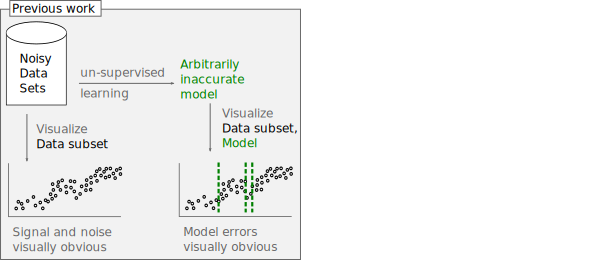
\includegraphics[height=0.5\textheight]{GenomicLearner-unsupervised.pdf}
\end{frame}

\begin{frame}
  \frametitle{GenomicLearner, an public web app for supervised interactive machine learning in genomic data}
  \includegraphics[height=0.5\textheight]{GenomicLearner-both.pdf}
\end{frame}


\begin{frame}
  \frametitle{Thanks for your attention!}

Any questions?

\hskip 1cm

%\includegraphics[width=\textwidth]{timeline-SteJustine}

 Write me at \alert{\texttt{toby.hocking@mail.mcgill.ca}} 

  % \vskip 1cm

  % timeline?

\end{frame}

\appendix

\begin{frame}
  \frametitle{Test error in three different experiments}
  \includegraphics[width=1.1\textwidth]{figure-test-error-dots-mean.pdf}
\end{frame}

\begin{frame}
  \frametitle{Accuracy benchmark: 10 manually labeled data sets}
  \url{http://cbio.ensmp.fr/~thocking/chip-seq-chunk-db/}
  \begin{itemize}
  \item We created 12,826 labels in 7 new data sets.
  \item 4 annotators (AM, TDH, PGP, XJ).
  \item 8 cell types.
  \item 37 H3K4me3 samples (sharp peak pattern).
  \item 29 H3K36me3 samples (broad peak pattern).
  \end{itemize}
  \vskip 1cm
  \url{http://tare.medisin.ntnu.no/chipseqbenchmark/}
  \begin{itemize}
  \item 3 data sets from another group's work in 2011.
  \item 3 transcription factors: SRF, NRSF, MAX.
  \item 2 replicates per transcription factor.
  \item Different protocol: label after peak calling.
  \end{itemize}
\end{frame}

\begin{frame}
  \frametitle{Train on some samples, test on others\\
(same histone mark and person)}
  \includegraphics[width=1.1\textwidth]{figure-test-H3K4me3-types.pdf}
\end{frame}

\begin{frame}
  \frametitle{Train on one histone mark, test on another\\
(same person and samples)}
  \includegraphics[width=1.1\textwidth]{figure-test-TDH-experiments.pdf}
\end{frame}

\begin{frame}
  \frametitle{Unsupervised algorithms inaccurate for 
    complex patterns}
  \begin{itemize}
  \item Domain expert (e.g. biologist) with prior knowledge manually codes an
    algorithm that recognizes the pattern.
  \item ``if the image $x$ has a dividing cell then predict
    $f(x)=\text{yes}$.''\\
    -- how to code that?
  \item ``if the copy number profile $x$ has a significant change of
    at least p-value $P$ in bins of size $B$, then predict
    $f(x)=\text{breakpoint}$.''\\
    -- sub-optimal parameter choices are inevitable.
    \end{itemize}
Disadvantages:
\begin{itemize}
  \item Need to find someone with programming experience AND domain expertise!
  \item Inaccurate: hard/impossible to manually write code that
    accurately recognizes complex patterns.
  \item Need to write a different algorithm for each pattern (0, 1, 2,
    %shoe, pants, 
    dividing cell, 
    normal cell,
    etc).
  \end{itemize}
\end{frame}

\section*{Learning a penalty function in maximum likelihood changepoint models}

\begin{frame}
  \frametitle{Supervised learning algorithm for breakpoint detection}
  H {\it et al.}, {\it ICML} 2013.
  \begin{itemize}
  \item New method for learning multi-feature linear penalty
    functions in maximum likehood changepoint models.
  \item Previous work: AIC/BIC/mBIC/etc (0 learned parameters)
    and scalar penalties (1 learned parameter).
  \item Contribution: convex optimization problem and learning
    algorithm for regression with censored outputs
    $(\underline L_i, \overline L_i)$.
  \item Results: improves breakpoint detection accuracy (cross-validation experiments).
  \end{itemize}
\includegraphics[width=0.4\textwidth]{screenshot-mmir-crop}
\includegraphics[width=0.4\textwidth]{screenshot-mmir-test-error}
\end{frame}

\begin{frame}
  \frametitle{useR2017 tutorial}
  
\end{frame}

\begin{frame}
  \frametitle{Nonlinear decision tree model}
  Drouin, Hocking, Laviolette {\it NIPS} 2017.
  \begin{itemize}
  \item Contribution: dynamic programming algorithm for learning a
    nonlinear decision tree model.
  \item Results: learns nonlinear patterns, improved
    breakpoint detection accuracy.
  \end{itemize}
%\includegraphics[width=\textwidth]{screenshot-mmit}

\includegraphics[width=\textwidth]{screenshot-mmit-learned}
\end{frame}

\begin{frame}
  \frametitle{Maximum Gaussian likelihood changepoint detection}

\includegraphics[width=\textwidth]{seg-mean}
\begin{align*}
    \minimize_{
  \mathbf m\in\RR^{n}
} &\ \ 
    \underbrace{
    \sum_{i=1}^n ( m_i - x_i)^2
}_{\text{fit the data}} + 
\underbrace{\lambda
\sum_{i=1}^{n-1} I(m_i\neq m_{i+1})}_{
\text{penalize number of changes}
}
\end{align*}

\begin{itemize}
\item Optimization variable $\mathbf m$ is the segment mean.
\item Minimizing the square loss corresponds to maximizing the
  Gaussian likelihood.
\item Penalty term encourages a model with few changes.
\item Penalty $\lambda=0$ means a change after every data point.
\item Penalty $\lambda=\infty$ means no changes.
\end{itemize}
\end{frame}

\begin{frame}
  \frametitle{Both HLA and markers selected in L1 regularized logistic regression
    model for predicting asthma }

  \begin{minipage}{0.39\linewidth}
    \begin{itemize}
    \item Right: many unused HLA alleles in the predictive model, one
      unused SNP.
    \item Below: SNP markers more accurate than HLA alleles.
    \end{itemize}
    \includegraphics[width=\textwidth]{figure-asthma-old}
  \end{minipage}
  \begin{minipage}{0.59\linewidth}
    \includegraphics[width=\textwidth]{figure-asthma-4folds}
  \end{minipage}
\end{frame}
 
\begin{frame}
  \frametitle{L1-regularized logistic regression model automatically selects relevant HLA features for each
    disease}

  \begin{itemize}
  \item HLA features predict some diseases more accurately than others.
  \item Different number of features selected per disease.
  \end{itemize}
  \includegraphics[width=\textwidth]{screenshot-ankylosing-spondylitis}

\scriptsize  \url{http://members.cbio.ensmp.fr/~thocking/figure-asthma-test-error/}
\end{frame}

\begin{frame}
  \frametitle{Models trained on labels from one person\\
predict accurately for another person\\
    (same histone mark and samples)}
  \includegraphics[width=1.1\textwidth]{figure-test-H3K4me3-annotators.pdf}

  Test error in four-fold cross-validation.
\end{frame}

% \begin{frame}
%   \frametitle{Multi-state changepoint model for neuro spike train
%     data}
%   Autoregressive single-state changepoint detection model (always
%   decreasing) Jewell and Witten, arXiv:1703.08644.

%   \includegraphics[width=0.45\textwidth]{Screenshot-neuro-spike-train}
%   \includegraphics[width=0.45\textwidth]{Screenshot-three-states}
% \end{frame}

\section*{Collaborations: applications of 
machine learning to genomics}

\begin{frame}
  \frametitle{Predicting flu vaccine response from gene expression}
  \only<1>{
    \includegraphics[height=0.5\textheight]{Screenshot-flu-vaccine-heatmap}
  }
  \only<2>{
    \includegraphics[height=0.5\textheight]{Screenshot-flu-vaccine-heatmap-circled}
  }
  \only<2>{
    \includegraphics[height=0.5\textheight]{Screenshot-flu-vaccine-genes}
  }

\begin{itemize}
\item Collaboration with Maiko Narahara (Kyoto University).
\item Output: response 90 days after vaccination, $n=270$ people.
\item Inputs: gene expression on day 7 --- 323 probes (227 genes)
  different. Which are the most important?
\item<2> L1-regularized logistic regression model predicts accurately
  %(AUC=0.81) 
using only three key genes: SDC1, TXNDC5, CD38.
\item<2> SDC1=CD138, CD38 identify plasma cells in flow cytometry
  (machine learning identified known markers).
\end{itemize}

% http://members.cbio.mines-paristech.fr/~thocking/figure-Ab-intervals-variables-samples.png

% Finally, we identified three key genes (SDC1, TXNDC5, and CD38) that
% could predict antibody responses at day90 (r=0.61, AUC=0.81, error
% rate=25.9%).

% We evaluated antibody titer responses in two different methods, binary
% classification into responders and non-responders (R/NR
% classification), and titer response index (TRI) 10 . For binary
% classification, we considered a seroconversion as a positive
% response. The US Food and Drug Administration (FDA) defined a
% seroconversion for influenza vaccines as four-fold or more increase
% from the baseline titer, or when the baseline titer was below the
% detection limit (<10), post-vaccination titers of x40 or more
% 26. Then we defined a responder as a subject who exhibited
% seroconversion to at least one strain at a certain time point, and a
% non-responder otherwise. TRI is a quantitative index of responsiveness
% relative to the baseline titers, which aggregates titer changes for
% three strains and different measurement methods 10 . We calculated
% titer response index as described previously except that we did not
% have neutralization titer measurements 10 .  The TRI scores were
% calculated with the 270 subjects who passed the exclusion criteria
% above.

% We identified 323 probes, or 227 unique genes, that were significantly
% associated with at least one of the antibody response phenotypes by
% FDR < 5%: 22, and 225 genes (DEGs) were associated with Day1 TRI,
% and Day90 TRI, respectively, and no genes were associated with Day7
% TRI (Figure 3A, Table S6-S7). 41 out of 44 probes associated with Day1
% TRI were also associated with Day90 TRI, and the P values for
% significant probes were correlated (Figure S8). But the signs of
% effect sizes for these probes were all negative for Day1 TRI (higher
% TRI scores at day1 were associated with lower expression fold
% changes at day7), and all positive for Day90 TRI.

% We showed that antibody responses at day90 could be effectively
% predicted by day7 expression of three genes (SDC1, CD38, and TXNDC5)
% without using expression data of immunoglobulin genes. These three
% genes were all also found in the DEGs. CD38 and TXNDC5 were clustered
% in the cluster 1, and SDC1 was in cluster 2 (Figure 3B). SDC1 is also
% known as CD138. Interestingly CD138 and CD38 proteins are the cell
% surface markers that are commonly used to identify plasma cells in
% flow cytometry. Therefore the machine learning approach successfully
% identified known markers for plasma cells without using a priori
% knowledge at all.

% TXNDC5 is known to suppress apoptosis and up-regulated in various
% cancers 78 ; however, its function in the immune system is
% unknown. Our results suggest a strong involvement of TXNDC5 in
% antibody responses.  Because TXNDC5 protein is considered to localize
% in the endoplasmic reticulum 79 , it might possibly involve in
% secretion of antibodies or cytokines, or transportation of endogenous
% antigens to present via Class I MHC. Regarding that TXNDC5 was chosen
% with two plasma cell marker genes, it might also function in plasma
% cells, and therefore, we speculate that it plays an important role
% particularly in antibody secretion in plasma cells.

\end{frame}

\begin{frame}
  \frametitle{Predicting autoimmune disease based on genetic variants}
  \includegraphics[height=0.4\textheight]{Screenshot-asthma-pvalues}
\only<2>{
  \includegraphics[height=0.4\textheight]{figure-asthma-old}
}
  \begin{itemize}
  \item Collaboration with Audrey Grant (McGill University).
  \item Output: asthma for $n=120286$ UK BioBank participants (genome
    wide association study).
  \item Inputs: SNP markers and HLA alleles, which are more
    predictive?
  \item<2> SNP markers are more predictive (model trained on HLA only
    is less accurate).
  \item<2> 31/32 SNP markers selected in L1-regularized logistic
    regression model (1 SNP marker not used).
  % \item white UK citizens, aged 40-70.
  % \item Genotyped using microarrays, 32 markers selected using
  %   univariate logistic regression test, 328 HLA alleles imputed.
  \end{itemize}
\end{frame}

% \begin{frame}
%   \frametitle{Machine learning setup for variant prioritization}
%   \begin{itemize}
%   \item $x\in\mathbb R^p$ = vector of scores from 
%     annotation programs (evolutionary conservation, biochemical
%     modeling, etc).
%   \item $f(x)\in\{0,1\}$ for predicting whether the variant is
%     pathogenic (1) or benign (0).
%   \item Existing methods to learn $f$: L1-regularized logistic
%     regression, random forests, boosting.
%   \item Scientific question: is the learned score more accurate than
%     the individual scores? Which features are relevant for predicting
%     pathogenicity?
%   \item Main novelty: train on ClinVar data set 2013--2015
%     (common/rare missense variants, 7059 benign, 4023 pathogenic)
%   \end{itemize}
% \end{frame}


\begin{frame}
  \frametitle{Predicting pathogenicity of genetic variants}
  \begin{itemize}
  \item Collaboration with Najmeh Alirezaie (McGill University).
  \item Output: pathogenicity of $n=11082$ variants in ClinVar.
  \item Inputs: scores based on conservation, biochemistry, etc.
  \item Learned ClinPred scores more accurate than individual scores.
  \item AF=Allele Frequency feature essential for optimal accuracy.
  \item All features selected in L1-regularized logistic regression.
  \end{itemize}
  \begin{center}
    \includegraphics[width=0.6\textwidth]{Screenshot-clinpred-auc}
  \end{center}
\end{frame}
 
\begin{frame}
  \frametitle{Two annotators provide consistent labels, but different
    precision}
  \includegraphics[width=1.1\textwidth]{screenshot-several-annotators}

  \begin{itemize}
  \item TDH peakStart/peakEnd more precise than AM peaks.
  \item AM noPeaks more precise than TDH no label.
  \end{itemize}
\end{frame}

\begin{frame}
  \frametitle{Joint peak calling pipeline for comparing samples}
\includegraphics[width=\textwidth]{PeakSegJoint-monocytes-up}

\begin{itemize}
\item Want to characterize active/inactive regions of the genome
  specifically for each cell type.
\item PeakSegJoint model predicts presence or absence of a common peak
  in multiple samples, Hocking and Bourque, arXiv:1506.01286,
  PeakSegJoint R package.
\end{itemize}
\end{frame}

\begin{frame}
  \frametitle{Example of peaks in heartbeat time series data}
  \includegraphics[width=0.4\textwidth]{Basil} B\'eb\'e Basil.
  \only<2>{
  \includegraphics[width=\textwidth]{figure-heartbeat-data-only}

  \scriptsize
  \url{https://github.com/tdhock/heartbeat/blob/master/heartbeat.mp3}
}
\end{frame}

\begin{frame}
  \frametitle{Unconstrained maximum likelihood changepoint
model does not satisfy up-down constraint}
  \includegraphics[width=\textwidth]{figure-heartbeat-unconstrained}

Optimal changepoints and means for $K=35$ segments.
\end{frame}
 
\begin{frame}
  \frametitle{Up-down constrained changepoint
model (PeakSeg) is interpretable in terms of heartbeats}
  \includegraphics[width=\textwidth]{figure-heartbeat-PeakSeg}

Optimal changepoints and means for $K=35$ up-down segments.
\end{frame}

\begin{frame}
  \frametitle{Can measure heartbeat duration}
  \includegraphics[width=\textwidth]{figure-heartbeat}
\end{frame}
 

\end{document}

 